%\IfFileExists{headerAB.tex}{\documentclass[a4paper,makeidx,envcountchap,graybox,deutsch,ngerman,sectrefs]{svmono}
%\documentclass[envcountchap,graybox,deutsch,sectrefs]{svmono}
%%%%% eigene tempor�re Abk�rzungsliste, f�r die Zeit, bis einheitliche Schreibungen bestehen
\usepackage{tempshort}
%%  Von Springer empfohlene Pakete %% 
%%\documentclass[envcountsect,graybox,deutsch,sectrefs]{svmono}
\usepackage{chapterbib}
\usepackage{type1cm}
\usepackage[ansinew]{inputenc}
\usepackage{babel}
\usepackage[pdftex]{graphicx}  %PDF-Vektorgrafiken einbinden
\usepackage{newtxtext}         %Typischer Springer-Font
\usepackage{newtxmath}
\usepackage{multicol}
\usepackage{multirow}
\usepackage[bottom]{footmisc}  %Platziert alle Fu�noten unten  
\usepackage[nobreak]{cite}
%\usepackage{biblatex}
\usepackage{cancel}
\usepackage[absolute]{textpos}
\usepackage{pdflscape}
\usepackage{graphicx}
\usepackage{pdflscape}
\usepackage{ragged2e}
\usepackage[format=plain,
      justification=RaggedRight,
      singlelinecheck=false]
     {caption}
\usepackage{longtable}
%\usepackage{floatrow}
%\usepackage{mwe}
\usepackage[figuresright]{rotating}
\usepackage{bigints}
\let\laplace\relax  % Vermeidung der Fehlermeldung "\laplace already defined."
\usepackage{trfsigns}
%\usepackage{relsize}
\usepackage{tabulary}
%\usepackage{xcolor,colortbl}
%\usepackage[table]{xcolor}
\usepackage{blindtext}
%\usepackage{acronym}
%\usepackage{amsmath}
\usepackage{acro}
\usepackage{nomencl}


\usepackage{etoolbox}
%  Eigene Pakete %%
\usepackage{adjustbox}
\usepackage{wasysym}
\usepackage{gensymb}
\usepackage{float}
\usepackage{caption}
\usepackage[left=3cm, right=3cm, top=3cm, bottom=3cm, includeheadfoot]{geometry}

\usepackage{mathtools}   % Vermeidung der Fehlermeldung "Undefined control sequence \coloneqq."
% header and footer
\usepackage{fancyhdr}
\pagestyle{fancy}
\fancyhead{}
\fancyhead[LE,RO]\thepage
\renewcommand{\sectionmark}[1]{\markright{\thesection.\ #1}}
%\fancyhead[LO]{\nouppercase\leftmark}
%\fancyhead[RE]{\nouppercase\rightmark}
\fancyhead[LO]{\nouppercase\rightmark}
\fancyhead[RE]{\nouppercase\leftmark}
\fancyfoot{}
% svmono hat offenbar irgendwas merkw�rdig definiert, darum mu� hier verbreitert werden
%\addtolength\headwidth{25pt}
%\setlength{\headheight}{25pt}

%% Units
\usepackage{siunitx}
\sisetup{
  locale = US,
  per-mode = reciprocal, %symbol, % | reciprocal | fraction | ?
  exponent-product = \cdot,
  separate-uncertainty,
  %exponent-to-prefix,
  %prefixes-as-symbols = false,
  %list-units = brackets,% | single | repeat
  %range-units = brackets,% | single | repeat
  %multi-part-units = brackets,% | single | repeat
}
\usepackage{chngcntr}
\usepackage{booktabs}
\usepackage{slashed}
\usepackage{listings}
\usepackage{color} %red, green, blue, yellow, cyan, magenta, black, white
%\usepackage{color} %Einfache Farbendefinition -> von Graybox-Option ben�tigt
\usepackage{multirow}
\usepackage{longtable} %Tabellen �ber mehrere Seiten hinweg
\usepackage{framed} % von Graybox-Option ben�tigt
\usepackage[shortlabels]{enumitem} %Erweiterte Aufz�hloptionen
\usepackage{array}
\usepackage[xindy]{imakeidx} %Wortindex und Personenindex erstellen

\usepackage[hyphens]{url}
%\usepackage[breaklinks,colorlinks=true,linkcolor=black,urlcolor=blue,citecolor=black,filecolor=green,hyperfootnotes=false]{hyperref}
\usepackage[                                    %Hyperref erstellt ein Bookmark/Lesezeichen im PDF. siehe https://www.namsu.de/Extra/pakete/Hyperref.html
bookmarksopen=true,															%Das Lesezeichen ist ge�ffnet beim �ffnen der PDF.
bookmarksnumbered=true,                         %Zahlen werden im Bookmark angezeigt.   
plainpages=false,
pdfpagelabels,
colorlinks=true,                                %Links werden farbig dargestellt.
linkcolor=black, citecolor=black, urlcolor=cyan %Farben definieren.
]{hyperref}                                     %Sollte als letztes eingebunden werden, da es sehr viele Verweise und �nderungen erzeugt. Das Packet ist sehr stark, aber auch umfangreich ist. 
\pdfminorversion=5

\usepackage{hypcap}
\usepackage[record,section=section,stylemods={mcols},automake]{glossaries-extra}
\usepackage{glossary-longextra}
\setglossarystyle{long-name-sym-desc-loc}
\setabbreviationstyle[acronym]{long-short}

\definecolor{killA}{rgb}{.7,.3,.3}
\newcommand\killA[1]{\bgroup\color{killA}{\cancel{#1}}\egroup}
\newcommand\killB[1]{\bgroup\color{cyan!30!black}{\cancel{#1}}\egroup}
% typographisch korrekte Abk�rzungen (needs to be loaded after hyperref)
\usepackage{abbrev}
\newglossary*{bew}{Glossar}
\newglossary*{hm}{Glossar}
\newglossary*{adyn}{Glossar}
\newglossary*{kontmech}{Glossar}
\newglossary*{aero}{Glossar}
\newglossary*{edyn}{Glossar}
\newglossary*{srt}{Glossar}
\newglossary*{spo}{Glossar}
\newglossary*{optbas}{Glossar}
\newglossary*{optger}{Glossar}
\newglossary*{optatm}{Glossar}
\GlsXtrLoadResources[src={bew/gloss},type=bew]
\GlsXtrLoadResources[src={hm/gloss},type=hm]
\GlsXtrLoadResources[src={adyn/gloss},type=adyn]
\GlsXtrLoadResources[src={kontmech/gloss},type=kontmech]
\GlsXtrLoadResources[src={aero/gloss},type=aero]
\GlsXtrLoadResources[src={spo/gloss},type=spo]
\GlsXtrLoadResources[src={edyn/gloss},type=edyn]
\GlsXtrLoadResources[src={srt/gloss},type=srt]
\GlsXtrLoadResources[src={optbas/gloss},type=optbas]
\GlsXtrLoadResources[src={optger/gloss},type=optger]
\GlsXtrLoadResources[src={optatm/gloss},type=optatm]
\glssetcategoryattribute{bew}{indexname}{true}
%\renewcommand\index\newterm
%\newcolumntype{g}[1]{>{\RaggedRight\hspace{0pt}}p{#1}}
%\renewcommand\glslongextraNameAlign{g}
\renewcommand\glslongextraLocationAlign{@{\ ~\ }>{\raggedright}p{\glspagelistwidth}}
\definecolor{gls}{rgb}{.4,.4,.5}
\renewcommand*{\glstextformat}[1]{\textcolor{gls}{#1}}

%Absatzregeln
\clubpenalty = 30000 %Keine einzelnen Absatzzeilen
\widowpenalty = 30000
\setlength{\parindent}{0em} 
\newcolumntype{L}[1]{>{\raggedright\arraybackslash}p{#1}}
\newcolumntype{C}[1]{>{\centering\arraybackslash}p{#1}}
\newcolumntype{R}[1]{>{\raggedleft\arraybackslash}p{#1}}

\usepackage{xstring}

\newcommand\mfile[2]{%
\saveexpandmode\noexpandarg
\StrSubstitute{#2}{_}{\_}[\tmpname]
\restoreexpandmode
\href{MatlabDateien/\chapname/#1\tmpname}{\tmpname}}

%%% Hyperlinks zu MATLAB Dateien
%\newcommand\mlref[1]{\mfile{}{#1}}
%\newcommand\mlinclref[1]{\mfile{IncludeFolder/}{#1}}
%\newcommand\mldataref[1]{\mfile{Data/}{#1}}

%%% .. f�r ein Verzeichnis hoch
%%% . f�r aktuelle Verzeichnis
%% lokal: MatlabDateien/bew
%\newcommand\mlbewref[1]{\href{MatlabDateien/bew/#1}{#1}}
%% git: https://github.com/sn-code-inside/fingeruebungen-physik/tree/main/bew
\newcommand{\mlrefwithindex}[2]{%
  \index[mfiles]{#2}%   <-- Eintrag im M-File-Index mit aktueller Seitenzahl
  \href{https://github.com/sn-code-inside/fingeruebungen-physik/tree/main/#1/#2}{#2}%
}


%\newcommand\mlbewref[1]{\href{https://github.com/sn-code-inside/fingeruebungen-physik/tree/main/bew/#1}{#1}}
%\newcommand\mlbewdref[1]{\href{https://github.com/sn-code-inside/fingeruebungen-physik/tree/main/bew/Data/#1}{#1}}
%\newcommand\mlbewiref[1]{\href{https://github.com/sn-code-inside/fingeruebungen-physik/tree/main/bew/IncludeFolder/#1}{#1}}
%\newcommand\mlkontmechref[1]{\href{https://github.com/sn-code-inside/fingeruebungen-physik/tree/main/kontmech/#1}{#1}}
%\newcommand\mlkontmechdref[1]{\href{https://github.com/sn-code-inside/fingeruebungen-physik/tree/main/kontmech/Data/#1}{#1}}
%\newcommand\mlkontmechiref[1]{\href{https://github.com/sn-code-inside/fingeruebungen-physik/tree/main/kontmech/IncludeFolder/#1}{#1}}
%\newcommand\mlhmref[1]{\href{https://github.com/sn-code-inside/fingeruebungen-physik/tree/main/hm/#1}{#1}}
%\newcommand\mlhmdref[1]{\href{https://github.com/sn-code-inside/fingeruebungen-physik/tree/main/hm/Data/#1}{#1}}
%\newcommand\mlhmiref[1]{\href{https://github.com/sn-code-inside/fingeruebungen-physik/tree/main/hm/IncludeFolder/#1}{#1}}
%\newcommand\mladynref[1]{\href{https://github.com/sn-code-inside/fingeruebungen-physik/tree/main/adyn/#1}{#1}}
%\newcommand\mladyndref[1]{\href{https://github.com/sn-code-inside/fingeruebungen-physik/tree/main/adyn/Data/#1}{#1}}
%\newcommand\mladyniref[1]{\href{https://github.com/sn-code-inside/fingeruebungen-physik/tree/main/adyn/IncludeFolder/#1}{#1}}
%\newcommand\mledynref[1]{\href{https://github.com/sn-code-inside/fingeruebungen-physik/tree/main/edyn/#1}{#1}}
%\newcommand\mledyndref[1]{\href{https://github.com/sn-code-inside/fingeruebungen-physik/tree/main/edyn/Data/#1}{#1}}
%\newcommand\mledyniref[1]{\href{https://github.com/sn-code-inside/fingeruebungen-physik/tree/main/edyn/IncludeFolder/#1}{#1}}
%\newcommand\mloptbasref[1]{\href{https://github.com/sn-code-inside/fingeruebungen-physik/tree/main/optbas/#1}{#1}}
%\newcommand\mloptbasdref[1]{\href{https://github.com/sn-code-inside/fingeruebungen-physik/tree/main/optbas/Data/#1}{#1}}
%\newcommand\mloptbasiref[1]{\href{https://github.com/sn-code-inside/fingeruebungen-physik/tree/main/optbas/IncludeFolder/#1}{#1}}
%\newcommand\mloptspezref[1]{\href{https://github.com/sn-code-inside/fingeruebungen-physik/tree/main/optspez/#1}{#1}}
%\newcommand\mloptspezdref[1]{\href{https://github.com/sn-code-inside/fingeruebungen-physik/tree/main/optspez/Data/#1}{#1}}
%\newcommand\mloptspeziref[1]{\href{https://github.com/sn-code-inside/fingeruebungen-physik/tree/main/optspez/IncludeFolder/#1}{#1}}

\newcommand\mlbewref[1]{\mlrefwithindex{bew}{#1}}
\newcommand\mlbewdref[1]{\mlrefwithindex{bew/Data}{#1}}
\newcommand\mlbewiref[1]{\mlrefwithindex{bew/Include}{#1}}
\newcommand\mlkontmechref[1]{\mlrefwithindex{kontmech}{#1}}
\newcommand\mlkontmechdref[1]{\mlrefwithindex{kontmech/Data}{#1}}
\newcommand\mlkontmechiref[1]{\mlrefwithindex{kontmech/Include}{#1}}
\newcommand\mlhmref[1]{\mlrefwithindex{hm}{#1}}
\newcommand\mlhmdref[1]{\mlrefwithindex{hm/Data}{#1}}
\newcommand\mlhmiref[1]{\mlrefwithindex{hm/Include}{#1}}
\newcommand\mladynref[1]{\mlrefwithindex{adyn}{#1}}
\newcommand\mladyndref[1]{\mlrefwithindex{adyn/Data}{#1}}
\newcommand\mladyniref[1]{\mlrefwithindex{adyn/Include}{#1}}
\newcommand\mledynref[1]{\mlrefwithindex{edyn}{#1}}
\newcommand\mledyndref[1]{\mlrefwithindex{edyn/Data}{#1}}
\newcommand\mledyniref[1]{\mlrefwithindex{edyn/Include}{#1}}
\newcommand\mlsrtref[1]{\mlrefwithindex{edyn}{#1}}
\newcommand\mlsrtdref[1]{\mlrefwithindex{srt/Data}{#1}}
\newcommand\mlsrtiref[1]{\mlrefwithindex{srt/Include}{#1}}
\newcommand\mloptbasref[1]{\mlrefwithindex{optbas}{#1}}
\newcommand\mloptbasdref[1]{\mlrefwithindex{optbas/Data}{#1}}
\newcommand\mloptbasiref[1]{\mlrefwithindex{optbas/Include}{#1}}
\newcommand\mloptgerref[1]{\mlrefwithindex{optger}{#1}}
\newcommand\mloptgerdref[1]{\mlrefwithindex{optger/Data}{#1}}
\newcommand\mloptgeriref[1]{\mlrefwithindex{optger/Include}{#1}}
\newcommand\mloptatmref[1]{\mlrefwithindex{optatm}{#1}}
\newcommand\mloptatmdref[1]{\mlrefwithindex{optatm/Data}{#1}}
\newcommand\mloptatmiref[1]{\mlrefwithindex{optatm/Include}{#1}}


\newcommand\mlcmd[1]{\textcolor{cyan}{\texttt{#1}}}

%Grafikregeln
\graphicspath{{hm/graphs/}
							{bew/graphs/}
							{kontmech/graphs/}
							{hm/graphs/}
							{adyn/graphs/}
							{edyn/graphs/}
							{srt/graphs/}
							{kontmech/graphs/}
							{spo/graphs/}
							{aero/graphs/}
							{optbas/graphs/}
							{optger/graphs/}
							{optatm/graphs/}
							{solman/graphs/}}
\DeclareGraphicsExtensions{.pdf, .png, .jpg, .jpeg}
\def\figname{Abb}
\newcommand\figref[1]{\figname.\ \ref{abb:#1}}
\usepackage[labelfont=bf]{caption}

\usepackage{tocloft}
\usepackage{etoc}
\setlength\cftfignumwidth{30pt}

% Flatterrand links
\cftsetindents{chapter}{0em}{4em}
\cftsetindents{section}{1.5em}{4em}
\cftsetindents{subsection}{3.8em}{4em}

% flacher Rand links
%\cftsetindents{chapter}{0em}{4em}
%\cftsetindents{section}{0em}{4em}
%\cftsetindents{subsection}{0em}{4em}

\newcommand\partitle[1]{
\addcontentsline{toc}{part}{#1}
\begin{titlepage}
  %\vskip 60%\p@
  \begin{center}
    {\LARGE Finger�bungen der Physik -- #1 \par}
    \vskip 3em%
    {\large Michael Kaschke und Holger Cartarius\par}
  \end{center}
\end{titlepage}
}

%\newcommand\mlref[1]{\href{\chapname/matlab/#1}{#1}}
%\newcommand\mlinclref[1]{\href{\chapname/matlab/IncludeFolder/#1}{\color{cyan}{#1}}}

%Neue Kommandos
\def\eg{e.\,g.\  \ignorespaces}     %e.g. (im Englischen Dokument)
\newcommand{\lk}{\left(}        %gro�e runde Klammer (links)
\newcommand{\rk}{\right )}      %gro�e runde Klammer (rechts)
\newcommand{\lgk}{\left \{}     %gro�e geschweifte Klammer (links)
\newcommand{\rgk}{\right \}}    %gro�e geschweifte Klammer (rechts)
\newcommand{\lek}{\left [}      %gro�e eckige Klammer (links)
\newcommand{\rek}{\right ]}     %gro�e eckige Klammer (rechts)
\newcommand{\anf}[1]{\glqq#1\grqq}    %Deutsche Anf�hrungszeichen: \anf{}
\newcommand{\defined}{:=}				%Definition
\newcommand{\curl}{\text{\textbf{rot}}\,}	%Rotation-Operator curl()
\newcommand{\ket}[1]{|#1\rangle}		%Quantenmechanischer Zustand
\newcommand{\curvelintri}{\,\overset{\blacktriangle}{\smallfrown}}
\newcommand{\straighttri}{\blacktriangle}
\newcommand{\UT}{\text{UT}}
\newcommand{\UTC}{\text{UTC}}
\newcommand{\JD}{\text{JD}}
\newcommand{\JDE}{\text{JDE}}
\newcommand{\MJD}{\text{MJD}}
\newcommand{\TDT}{\text{TDT}}
\newcommand{\TT}{\text{TT}}
\newcommand{\NVS}{\text{Navier-Stokes-Gleichungen}}
\newcommand{\MWG}{\text{Max\-well-Gleich\-ungen}}
\newcommand{\HG}{\text{Helm\-holtz-Glei\-chung}}
\newcommand{\sHG}{\text{ska\-lare Helm\-holtz-Glei\-chung}}
\newcommand{\vHG}{\text{vek\-to\-riel\-le Helm\-holtz-Glei\-chung}}
\newcommand{\sHGn}{\text{ska\-laren Helm\-holtz-Glei\-chung}}
\newcommand{\vHGn}{\text{vek\-to\-riel\-len Helm\-holtz-Glei\-chung}}
\newcommand{\SRT}{\text{Spezielle Relativit�tstheorie}}
\newcommand{\sRT}{\text{speziellen Relativit�tstheorie}}
\newcommand{\EMW}{\text{Elek\-tro\-magne\-tische Wellen}}
\newcommand{\eMW}{\text{elek\-tro\-magne\-tische Wellen}}
\newcommand{\eme}{\text{elektromagnetische}}
\newcommand{\EMF}{\text{Elektromagnetisches Feld}}
\newcommand{\eMF}{\text{elektromagnetischen Feld}}
\newcommand{\RT}{\text{Relativit�tstheorie~}}
\newcommand{\au}{\mathrm{AE}}
\newcommand{\ET}{\text{ET}}
\newcommand{\TAI}{\text{TAI}}
\newcommand{\GMST}{\text{GMST}}
\newcommand{\LMST}{\text{LMST}}
\newcommand{\MESZ}{\text{MESZ}}
\newcommand{\KOS}{\text{Koordinatensystem }}
\newcommand{\DGL}{\text{Differentialgleichung }}
\newcommand{\NA}{\text{NA}}
\newcommand{\uA}{\text{u}}  %atomare Masseneinheit
\newcommand{\MOZ}{\text{MOZ}}
\newcommand{\grad}{\text{\textbf{grad}}\,}	%Gradient-Operator grad()
\newcommand{\uproman}[1]{\uppercase\expandafter{\romannumeral#1}}
\newcommand{\lowroman}[1]{\romannumeral#1\relax}
\newcommand\todo[1]{\textcolor{red}{TODO: #1}}
\renewcommand{\=}[1]{\stackrel{\text{#1}}{=}}  %Schrift �ber Gleich-Zeichen
\renewcommand{\d}{\partial}
\newcommand{\abs}[1]{\left\vert#1\right\vert}            %Betragsklammern
\renewcommand{\Re}{\mathrm{Re}}                          %Realteil
\renewcommand{\Im}{\mathrm{Im}}                          %Imagin�rteil
\renewcommand{\im}{\mathrm{i}}                           %Imagin�re Einheite
\newcommand{\epsi}{\varepsilon} 
\renewcommand{\exp}{\mathrm{exp}}                        %Exponentialfunktion
\newcommand{\keff}{k_\text{eff}}
\newcommand{\con}{\text{const}}
\newcommand{\conv}{\vec{const}}
\newcommand{\nL}{n_\text{L}}    %n_L Brechungsindex Linse
\newcommand{\PL}{\mathcal{P}_}  %Legendre Polynome
\newcommand{\Pl}{\mathcal{P}}   %Legendre Polynome �ltere Variante 
\newcommand{\RB}{\mathcal{R}}   %Allgemeine Radial_Bessel_Funktion
\newcommand{\ve}{\vec{e}}   %Einheitsvektor
\newcommand{\vr}{\vec{r}}   %Ortsvektor
\newcommand{\vk}{\vec{k}}   %Wellenzahlvektor
\newcommand{\vp}{\vec{p}}   %Impulsvektor
\newcommand\PLZ[2]{\mathcal{P}_{#1}^{#2}}  %zugeordnete Legendre-Funktionen 

\DeclareRobustCommand{\sB}{\tilde{\mathcal{J}}} %sph�rische Bessel-Funktion 
\DeclareRobustCommand{\sNeu}{\tilde{\mathcal{N}}} %sph�rische Neumann-Funktion 
\DeclareRobustCommand{\sHank}{\tilde{\mathcal{H}}} %sph�rische Hankel-Funktion 

\newcommand\BFu {\mathcal{J}} % Bessel-Funktion 
\newcommand\NeuFu {\mathcal{N}} % Neumann-Funktion 
\newcommand\HankFu {\mathcal{H}} % Hankel-Funktion

\newcommand\B {\mathcal{J}_\ell\lk kr \rk} % Bessel-Funktion mit \ell
\newcommand\jB {\tilde{\mathcal{J}}_\ell\lk kr \rk} %sph�rische Bessel-Funktion mit \ell
\newcommand\Neu {\mathcal{N}_\ell\lk kr \rk} %Neumann-Funktion mit \ell
\newcommand\Hank {\mathcal{H}_\ell\lk kr \rk} %Hankel-Funktion mit \ell

\newcommand{\tu}{~~\text{und}~~}   %und in Gleichungen
\newcommand{\pdv}{\frac{~\d}{\d}\frac~}   %partielle Ableitung in LGL
\newcommand{\pdV}{\frac{\d}{\d}\frac}   %partielle Ableitung in LGL

%% JK commands
 \newcommand{\CP}{\cos\phi}   
 \newcommand{\SP}{\cos\phi}   
 \newcommand{\CT}{\cos\theta}   
 \newcommand{\ST}{\sin\theta}   
 \newcommand{\U}{U \left(r,\theta\right)}

\newcommand{\artanh}{\mathrm{artanh}}
\newcommand{\textqed}{\hfill ~ $\square$}
\newcommand{\mmqed}{\tag*{$\square$}}
\newcommand{\tensor}[1]{\mathbb{#1}}			 %Tensorvariable, Matrixvariable

\newcommand{\fa}{(\textbf{a})~}
\newcommand{\fb}{(\textbf{b})~}
\newcommand{\fc}{(\textbf{c})~}
\newcommand{\fd}{(\textbf{d})~}
\newcommand{\fe}{(\textbf{e})~}
\newcommand{\ff}{(\textbf{f})~}
\newcommand{\fg}{(\textbf{g})~}

\newcommand{\iF}{im Folgenden~}
\newcommand{\iA}{im Allgemeinen~}

\newcommand{\zmu}{\mathsf{\times}~}


\newcommand{\hatr}{\hat{\vec{r}}}
\newcommand{\hbtr}{\left| \hat{\vec{r}} \right|}

\DeclareMathOperator\res{Res}
\DeclareMathOperator{\sech}{sech}
\DeclareMathOperator\sgn{sgn}
% f�r Appendix - MATLAB und Python Referenz
\newcommand{\py}{Python}
\newcommand{\rotv}{\vec{rot}\,}
\newcommand{\gradv}{\vec{grad}\,}
\newcommand{\nablav}{\vec{\nabla}\,}
\newcommand{\divv}{\mathrm{div}\,}
\newcommand{\ceil}{\mathrm{ceil}}
\newcommand{\sinc}{\mathrm{sinc}}
\newcommand{\diag}{\mathrm{diag}}
\newcommand{\sign}{\mathrm{sign}}
\newcommand{\length}{\mathrm{length}}
\newcommand{\sort}{\mathrm{sort}}
\newcommand{\summ}{\mathrm{sum}}
\newcommand{\asin}{\mathrm{asin}}
\newcommand{\acos}{\mathrm{acos}}
\newcommand{\atan}{\mathrm{atan}}
\newcommand{\prodd}{\mathrm{prod}}
\newcommand{\median}{\mathrm{mediab}}
\newcommand{\mean}{\mathrm{mean}}
\newcommand{\std}{\mathrm{std}}
\newcommand{\eye}{\mathrm{eye}}
\newcommand{\zeros}{\mathrm{zeros}}
\newcommand{\ones}{\mathrm{ones}}
\newcommand{\rand}{\mathrm{rand}}
\newcommand{\inline}{\mathrm{inline}}
\newcommand{\modd}{\mathrm{mod}}
\newcommand{\floor}{\mathrm{floor}}
\newcommand{\round}{\mathrm{round}}
\newcommand{\rem}{\mathrm{rem}}
\newcommand{\sqrtt}{\mathrm{sqrt}}
\newcommand{\triu}{\mathrm{triu}}
\newcommand{\tril}{\mathrm{tril}}
\newcommand{\size}{\mathrm{size}}
\newcommand{\dett}{\mathrm{det}}
\newcommand{\rect}{\mathrm{rect}}
\newcommand{\OTF}{\mathrm{OTF}}
\newcommand{\inv}{\mathrm{inv}}
\newcommand{\rank}{\mathrm{rank}}
\newcommand{\rref}{\mathrm{rref}}
\newcommand{\eig}{\mathrm{eig}}
\newcommand{\poly}{\mathrm{poly}}
\newcommand{\lu}{\mathrm{lu}}
\newcommand{\qr}{\mathrm{qr}}
\newcommand{\R}{\mathbb{R}}
\newcommand{\quaddd}{\mathrm{quad}}
\newcommand{\fzero}{\mathrm{fzero}}
\newcommand{\roots}{\mathrm{roots}}
\newcommand{\odezd}{\textcolor{mygreen}{\texttt{ode23}}}
\newcommand{\odevf}{\textcolor{mygreen}{\texttt{ode45}}}
\newcommand{\odeeds}{\textcolor{mygreen}{\texttt{ode13s}}}
\newcommand{\odeefs}{\textcolor{mygreen}{\texttt{ode15s}}}
\newcommand{\ddezd}{\textcolor{mygreen}{\texttt{dde23}}}
\newcommand{\onlineZ}{online verf�gbaren Zusatzmaterialien{}}
%\newcommand{\MKc}{\url{https://kaschke-medtec.de/fingeruebungen.html}{}}
\newcommand{\MKc}{\url{https://www.fingeruebungen-physik.de}{}}
\newcommand{\linklsg}{\href{https://www.fingeruebungen-physik.de}{\textcolor{blue} {$\rightarrow$ L�sungsteil.}}}
\newcommand{\githubSN}{\url{https://github.com/sn-code-inside/fingeruebungen-physik}{}\,\,}

\newcommand{\PSF}{\mathrm{PSF}} %PSF
\newcommand{\FT}{\mathcal{F}} %Fourier-Transformierte
\newcommand{\iFT}{\mathcal{F}^{-1}} %inverse Fourier-Transformierte
\newcommand{\KFF}{Kugel\-fl�\-chen\-funk\-tio\-nen~} %Kugelfl�chenfunktionen
\newcommand{\HH}{Hansen-\-Har\-mo\-nics~} %Hansen-Harmonics
\newcommand{\TE}{^\mathrm{(TE)}} %Transversal elektrisch
\newcommand{\TM}{^\mathrm{(TM)}} %Transversal magnetisch
\newcommand{\sumlm}{\sum\limits_{l=0}^\infty \sum\limits_{m=-l}^l} %Summe �ber l,m KFF

% Aufz�hlung der L�sungen der Teilaufgaben
\newlist{subprobs}{enumerate}{1}
\setlist[subprobs]{
  label= \textbf{\textit{Teilaufgabe}} \textbf{\textit{\arabic*:}} \protect\thissubprob,
  ref=\arabic*, itemsep=\baselineskip, align=left}
\newcommand{\subprob}[1]{
  \def\thissubprob{\textbf{\textit{#1}}}\item ~\vspace{0.2\baselineskip} \newline}


%%%%%%%%%%%%%%%%%%%%%%%%%%%%%%%%%%%%%%%%%%%%%%%%%%%%%%%%%%%%%%%%%%%%%%%%
% Abk�rzungen, Formelzeichen

\makenomenclature
\renewcommand{\nomname}{}

\renewcommand{\nomgroup}[1]{%
  \ifthenelse{\equal{#1}{L}}{\item[]\vspace{0.4\baselineskip}\item[\bfseries Lateinische Symbole]}{%
  \ifthenelse{\equal{#1}{G}}{\item[]\vspace{0.6\baselineskip}\item[\bfseries Griechische Symbole]}{%
  \ifthenelse{\equal{#1}{O}}{\item[]\vspace{0.6\baselineskip}\item[\bfseries Indizes und Operatoren]}{}}}%
}

\newif\iffirstnomgroup
\firstnomgrouptrue

\renewcommand{\nomgroup}[1]{%
  \iffirstnomgroup
    \global\firstnomgroupfalse
  \else
    \item[]\vspace{0.6\baselineskip}%
  \fi
  \item[\bfseries
    \ifthenelse{\equal{#1}{L}}{Lateinische Symbole}{%
    \ifthenelse{\equal{#1}{G}}{Griechische Symbole}{%
    \ifthenelse{\equal{#1}{O}}{Indizes und Operatoren}{}}}%
  ]%
  \item[]\vspace{0.2\baselineskip}%
}

\setlength{\nomitemsep}{0.25\baselineskip}

\makeatletter
\renewenvironment{thenomenclature}[1][\nomlabelwidth]{%
  \nompreamble
  \setnomtableformat{lp{0.8\textwidth}sp{0.5\textwidth}@{}l}
  \setlength{\labelsep}{1.8em}
  \list{}{%
    \labelwidth#1%
    \leftmargin\labelwidth
    \advance\leftmargin\labelsep
    \itemsep\nomitemsep
    \let\makelabel\nomlabel
  }%
}{%
  \endlist
  \nompostamble
}
\makeatother

% Gemeinsame Breite der linken Spalte
\newlength{\verzlabelwidth}
\setlength{\verzlabelwidth}{2.5cm}


%%%%%%%%%%%%%%%%%%%%%%%%%%%%%%%%%%%%%%%%%%%%%%%%%%%%%%%%%%%%%%%%%%%%%%%%%%%%%%%%%%%%%%%%%%%%%%%%%%


\definecolor{mygreen}{RGB}{28,172,0} % color values Red, Green, Blue
\definecolor{myblue}{RGB}{28,28,172}
\definecolor{myyellow}{RGB}{237,162,13}
\definecolor{shadecolor}{gray}{0.95}
\definecolor{mylilas}{RGB}{170,55,241}

\renewenvironment{example}[1]{
\refstepcounter{example}\par\medskip
\begin{shaded} 
%\begin{samepage}
 
\noindent{\color{mygreen} \rule[3pt]{\textwidth}{0.3mm}}
\begin{tabular}{>{\arraybackslash}m{1cm}>{\arraybackslash}m{17cm}}

\includegraphics[width=8mm]{example.pdf}&
\noindent \textbf{\textit{Beispiel~\theexample: {#1}}}
\end{tabular}
\noindent{\color{mygreen} \rule[3pt]{\textwidth}{0.2 mm}}
%\end{samepage}
}{\end{shaded}
\vspace{-1cm}\noindent{\color{mygreen} \rule{\textwidth}{0.3 mm}}
} 

%%%%%%%%%%%%%%%%%%%%%%%%%%%%%%%%%%%%%%%%%%%%%%%%%%%%%%%%%%%%%%%

\newenvironment{infobox}[1]{
     \begin{shaded} 
     \begin{samepage}
\noindent{\color{myblue} \rule[3pt]{\textwidth}{0.3 mm}}
\begin{tabular}{>{\arraybackslash}m{1cm}>{\arraybackslash}m{17cm}}

\includegraphics[width=6mm]{info.pdf}&
%\noindent \textbf{\textit{~Infobox:~ {#1}}} 
\noindent \textbf{\textit{~ {#1}}} 
\end{tabular}
\noindent{\color{myblue} \rule[3pt]{\textwidth}{0.2 mm}}
     \end{samepage}
}{\end{shaded}
\vspace{-1cm}\noindent{\color{myblue} \rule{\textwidth}{0.3 mm}}
} 


\newenvironment{merksatz}[1]{
\begin{shaded} 
     %\begin{samepage}
\noindent{\color{myyellow} \rule[3pt]{\textwidth}{0.3 mm}}
\begin{tabular}{>{\arraybackslash}m{1cm}>{\arraybackslash}m{17cm}}

\includegraphics[width=6mm]{merke.pdf}&
%\noindent \textbf{\textit{~Merke:~ {#1}}}
\noindent \textbf{\textit{~ {#1}}}
\end{tabular}
\noindent{\color{myyellow} \rule[3pt]{\textwidth}{0.2 mm}}
     %\end{samepage}
}{\end{shaded}
\vspace{-1cm}\noindent{\color{myyellow} \rule{\textwidth}{0.3 mm}}
}

%%%%%%%%%%%%%%%%%%%%%%%%%%%%%%%%%%%%%%%%%%%%%%%%%%%%%%%%%%%%%%%


\newenvironment{nebenrechnungNeu}[1]{
\begin{shaded} 
     \begin{samepage}
\noindent{\color{black} \rule[3pt]{\textwidth}{0.3 mm}}
\begin{tabular}{>{\arraybackslash}m{1cm}>{\arraybackslash}m{17cm}}
%
\includegraphics[width=6mm]{nr.pdf}&

\includegraphics[width=6mm]{info.pdf}&
\noindent \textbf{\textit{~Nebenrechnung:~ {#1}}}
\end{tabular}
\noindent{\color{black} \rule[3pt]{\textwidth}{0.2 mm}}
     \end{samepage}
}{\end{shaded}
\vspace{-1cm}\noindent{\color{black} \rule{\textwidth}{0.3 mm}}
}

\newenvironment{nebenrechnung}[1]{
\begin{shaded} 
\begin{samepage}
\noindent\textbf{Nebenrechnung: \\} 
\noindent{\color{black} \rule{0.1\columnwidth}{0.2mm} \\}
\end{samepage}
}{\end{shaded}
\noindent{\color{black} \rule{0.1\columnwidth}{0.2mm} \\}
} % or snugshade
\definecolor{shadecolor}{gray}{0.95}
\definecolor{mygreen}{RGB}{28,172,0} % color values Red, Green, Blue
\definecolor{mylilas}{RGB}{170,55,241}


\lstset{language=Matlab,%
    %basicstyle=\color{red},
    %basicstyle={\linespread{0.9}\ttfamily},
    basicstyle=\footnotesize\ttfamily,
    breaklines=true,%
    morekeywords={matlab2tikz},
    keywordstyle={\small \color{mygreen}},%
    morekeywords=[2]{1}, keywordstyle=[2]{\small\color{black}},
    identifierstyle={\small \color{black}},%
    stringstyle={\small\color{mylilas}},
    commentstyle={\small\color{mylilas}},%
    showstringspaces=false,%without this there will be a symbol in the places where there is a space
    numbers=left,%
    numberstyle={\tiny \color{black}},% size of the numbers
    numbersep=9pt, % this defines how far the numbers are from the text
    emph=[1]{for,end,else,break, function},emphstyle=[1]\small \color{blue}, %some words to emphasise
    emph=[2]{odeset},emphstyle=[2]\small \color{mygreen}, %some words to emphasise
    %emph=[2]{word1,word2}, emphstyle=[2]{style},    
}

%\bibliographystyle{spphys.bst}

%Trennregeln f�r spezielle Worte
%\hyphenation{Fresnel \matlab �qui-nok-ti-um}

\DeclareSIUnit\erg{erg}
\DeclareSIUnit\cal{cal}
\DeclareSIUnit\celsius{C}
\DeclareSIUnit\m{M}
\DeclareSIUnit\kel{K^{-4}}

%Stichwort- und Personenverzeichnis
\makeindex[title=Stichwortverzeichnis] % Create the default index
\makeindex[name=personen,title=Personenverzeichnis] % Create an index named 'personen'
\newcommand{\indexp}[1]{\index[personen]{#1}}
\makeindex[name=mfiles,title=MATLAB-Skriptverzeichnis,columns=2]

% list of exercises
\newcommand{\loxname}{\Large �bungsverzeichnis}  % einheitliche Gr��e Large
\newlistof[chapter]{prob}{lox}\loxname
\newcommand\uebung[3][]{\label{prob:#2}%
\addcontentsline{lox}{prob}{\protect\numberline{}{\probRef{#2}:~#3#1}}%
\textbf{#1#3}\\[\baselineskip]}
\makeatletter
\renewcommand{\l@prob}{\@dottedtocline{1}{0em}{0em}}
\makeatother
\newcommand\einfach{\uebung[~$\ast$~~]}
\newcommand\mittel{\uebung[~$\ast\,\ast$~~]}
\newcommand\schwierig{\uebung[~$\ast\,\ast\,\ast$~~]}
\newcommand\zusatz{\uebung[~$\ast\,\ast\,\ast\,!$~~]}
%\newcommand\einfach{\uebung[~\textbf{*}~~]}
%\newcommand\mittel{\uebung[~\textbf{*\,*}~~]}
%\newcommand\schwierig{\uebung[~\textbf{*\,*\,*}~]}
%\newcommand\zusatz{\uebung[~\textbf{*\,*\,*\,!}~~]}
\usepackage[atend]{bookmark}
%\BookmarkAtEnd{%
%\bookmarksetup{startatroot}\bookmark[level=0,named=\loxname]{}}

% Einheitliche �berschrift
\newcommand\verzeichnisueberschrift[1]{\section*{#1}}
\newcommand\kapitel[1]{Kapitel \ref{kap:#1}}
\newcommand\kap[1]{Kap. \ref{kap:#1}}


% Acronyms

\acsetup{
  list/name     = Abk�rzungsverzeichnis,
  list/template = tabular
}

\DeclareAcronym{NASA}{short = NASA, long  = National Aeronautics and Space Administration}
\DeclareAcronym{ESO}{short = ESO, long  = European Southern Observatory}

\DeclareAcronym{ccd}{short = CCD, long  = Charge-Coupled Device}
\DeclareAcronym{otf}{short = OTF, long  = Optical Transfer Function}
\DeclareAcronym{tmm}{short = TMM, long  = Transfermatrix-Methode}
\DeclareAcronym{tmft}{short = TMFT, long  = Thin Film Matrix Theory}
\DeclareAcronym{ar}{short = AR, long  = Anti-Reflexion}
\DeclareAcronym{cgh}{short = CGH, long  = Computer Generated Hologramm}
\DeclareAcronym{grin}{short = GRIN, long  = Gradient Index}
\DeclareAcronym{vat}{short = VAT, long  = Value Averaging Theory}
\DeclareAcronym{fem}{short = FEM, long  =  Finite Elemente Methode}
\DeclareAcronym{rcwa}{short = RCWA, long  = Rigorous Coupled Wave Theory}
\DeclareAcronym{tdtd}{short = FDTD, long  = Finite Difference Time Domain}
\DeclareAcronym{adc}{short = ADC, long  = Analog-Digital-Converter}
\DeclareAcronym{psf}{short = PSF, long  = Punktspreizfunktion (Point Spread Function)}
\DeclareAcronym{apsf}{short = APSF, long  = Amplitudenpunktspreizfunktion (Amplitude Point Spread Function)}
\DeclareAcronym{fwhm}{short = FWHM, long  = Full Width Half Maximum}

\DeclareAcronym{pd}{short = PD, long  =  Photodiode}
\DeclareAcronym{pmt}{short = PMT, long  =  Photomultiplier Tube}
\DeclareAcronym{apd}{short = APD, long  =  Avalanche Photodiode}
\DeclareAcronym{spad}{short = SPAD, long  =  Single-Photon-Avalanche Photodiode}
\DeclareAcronym{spcd}{short = SPCD, long  =  Single-Photon-Count Detection}
\DeclareAcronym{cmos}{short = CMOS, long  =  Complementary Metal-Oxide-Semiconductor}
\DeclareAcronym{mcp}{short = MCP, long  =  Mikrokanalplatte (Micro Channel Plate)}
\DeclareAcronym{snr}{short = SNR, long  =  Signal-Rausch-Verh�ltnis (Signal Noise Ratio)}
\DeclareAcronym{lsm}{short = LSM, long  =  Laser-Raster-Mikroskopie (Laser-Scanning-Microscopy)}
\DeclareAcronym{ics}{short = ICS, long  =  Infinity Corrected System}
\DeclareAcronym{dic}{short = DIC, long  =  Differentielle Interferenzkontrast (Differential Interference Contrast)}

\DeclareAcronym{palm}{short = PALM, long  =  Photo-Activated Localization Microscopy}
\DeclareAcronym{sim}{short = SIM, long  =  Structured Illumination Microscopy}
\DeclareAcronym{sted}{short = STED, long  =  Stimulated Emission Depletion}
\DeclareAcronym{storm}{short = STORM, long  =  Stochastic Optical Reconstruction Microscopy}

\DeclareAcronym{aps}{short = APS, long  =  Advanced Photo System}
\DeclareAcronym{mft}{short = MFT, long  =  Micro Four Thirds}
\DeclareAcronym{dof}{short = DOF, long  =  Depth of Field}
\DeclareAcronym{fov}{short = FOV, long  =  Field ov View}
\DeclareAcronym{mp}{short = MP, long  =  Mega Pixel}



%-------------------------------------------------------
% Abk�rzungen
% ------------------------------------------------------
\begin{document}
% customize prob and sol in svmono
\makeatletter
%\counterwithin*{chapter}{part}

\spn@wtheorem{prob}{\bgroup\exercisename\egroup}{\bfseries}{\rmfamily}
\makeatother
\renewenvironment{sol}[1]{\par\addvspace{6pt}\noindent\phantomsection{\textbf{L�sung zu \ref{#1}}} \ignorespaces}{\par\addvspace{6pt}}
\newcommand\probRef[1]{�bung \ref{prob:#1}}
\renewcommand\probref[1]{\textbf{\probRef{#1}}}
\newcommand\lsgref[1]{L�sung \ref{lsg:#1}}

%\newcommand\sbullet[1][.5]{\mathbin{\vcenter{\hbox{\scalebox{#1}{$\bullet$}}}}}




\setcounter{table}{0}

}{}
%%%%%%%%%%%%%%%%%%%%%%%%%%%%%%%%%%%%%%%%%%%%%%%%%%%%%%%%%%%%%%%
%\addtocontents{toc}{\protect\setcounter{tocdepth}{-1}}% nichts zeigen bei Arbeitsbuch
\addtocontents{toc}{\protect\setcounter{tocdepth}{3}}% alles zeigen bei WorkBook

\chapter{Himmelsmechanik} \label{chap:hm}
\def\chapname{hm}
\bibliographystyle{spphys}
\begin{minipage}{0.5\textwidth}
\includegraphics[width=\textwidth]{Analemma.jpg}
\end{minipage}
\medskip
\begin{minipage}{0.5\textwidth}
\begin{flushright}
\small
\emph{Wenn das die Sternenkunst ist, will ich froh\\
Zu diesem heitern Glauben mich bekennen.\\
Es ist ein holder, freundlicher Gedanke,\\
Da� �ber uns, in unerme�nen H�hn,\\
Der Liebe Kranz aus funkelnden Gestirnen,\\
Da wir erst wurden, schon geflochten ward.\\}
\medskip
Friedrich von Schiller (1759--1805)\\
\medskip
\medskip
\emph{Alle Schwierigkeit der Physik \\
besteht n�mlich dem Anschein nach darin,\\
aus den Erscheinungen der Bewegung\\
die Kr�fte der Natur zu erforschen\\
und hierauf durch diese Kr�fte \\
die �brigen Erscheinungen zu erkl�ren.\\}
\medskip
Sir Isaac Newton (1643--1727)
\normalsize
\end{flushright}
\end{minipage}

\section{Motivation}\label{kap:hm_motivation}

Eine der wohl sch�nsten und zugleich erfolgreichsten Anwendungen der Mechanik ist die Himmelsmechanik, haben Menschen doch schon seit dem Altertum die mit vielen Harmonien, aber auch singul�ren Ereignissen ausgestattete \anf{Himmelsmaschine} beobachten, beschreiben, vermessen und eben auch berechnen k�nnen.
Aber erst Isaac Newton\indexp{Newton, Sir Isaac}\footnote{Sir Isaac Newton (1643--1727) war einer der bedeutendsten Naturforscher aller Zeiten. Er formulierte die Gravitations- und Bewegungsgesetze und entwickelte fast gleichzeitig mit dem deutschen Universalgelehrten Leibniz (1646--1716) die Infinitesimalrechnung. Newtons \emph{Principia} werden als eines der wichtigsten wissenschaftlichen Werke angesehen.} konnte in seinen \anf{Principia} \cite{Newton2010} im Jahr 1687 eine umfassende physikalische Theorie dieser beobachteten Ph�nomene geben.
In den folgenden Jahrhunderten besch�ftigten sich viele Mathematiker, Physiker und Astronomen mit Problemen der Himmelsmechanik, wobei der Begriff \emph{Himmelsmechanik} erstmals von Pierre Simon de Laplace\indexp{Laplace, Pierre-Simon (Marquis) de}\footnote{Pierre-Simon (Marquis) de Laplace (1749--1827) war ein franz�sischer Mathematiker, Physiker und Astronom. Sein Hauptwerk ist die \emph{Trait� de M�canique C�leste} (Abhandlung �ber die Himmelsmechanik). Er besch�ftigte sich auch mit Wahrscheinlichkeitstheorie und der L�sung von Differentialgleichungen.} gepr�gt wurde.
Obwohl die Newtonsche Theorie der Gravitation in ihren Grundgleichungen bestechend einfach ist, sind viele Konstellationen und Problemstellungen der Himmelsmechanik nicht geschlossen analytisch l�sbar, sondern m�ssen durch numerische Methoden, Reihenentwicklungen oder St�rungsrechnungen berechnet werden.
Damit wandert vieles der physikalischen Sch�nheit und Einfachheit ins Kabinett der (numerischen) Methoden der Spezialisten.
Das erkl�rt m�glicherweise auch, warum die Himmelsmechanik relativ selten Bestandteil des Curriculums im Physikstudium ist.
Das ist eigentlich schade, denn es gibt eine Reihe von Problemen, die mit gutem physikalischen Grundwissen f�r die meisten Situationen mit ausreichender Genauigkeit geschlossen oder zumindest n�herungsweise analytisch \bzw numerisch berechnet werden k�nnen und so gleichzeitig ein tieferes physikalisches Verst�ndnis erlauben.
Genauso schade ist es, dass die aus der Bewegung von Himmelsk�rpern resultierenden Ph�nomene wie ein Analemma\footnote{Das Titelbild ist ein Analemma, aufgenommen von Bertram H�nlinger und Michael Kaschke mit einem Objektiv ZEISS Classic Distagon 2.8/21 ZF.2. Die geographischen Koordinaten waren \ca \SI{48}\degree N / \SI{10}\degree O. Im Verlauf der Aufnahmen f�r das Analemma im Jahr 2015 wurde auch eine partielle Sonnenfinsternis beobachtet. Wir werden ein solches Analemma in \kap{zeitgleichung} berechnen und k�nnen anhand der Berechnung ermitteln, dass das Datum dieser Sonnenfinsternis der 20. M�rz 2015 war.} oder eine Sonnenfinsternis von vielen Physikern zwar erkl�rt, aber nicht berechnet werden k�nnen. 
Auch die genaue Berechnung eines �sthetisch immer wieder beeindruckenden Sonnenaufgangs verschlie�t sich den meisten Physikstudenten, obwohl das mathematisch-physikalische Handwerkszeug dazu aus dem Grundstudium vorhanden ist.

In einer Zeit, in der wegen der Lichtverschmutzung leider immer weniger Menschen die Ph�nomene der Himmelsmechanik am Nachthimmel in ihrer vollen Sch�nheit erleben k�nnen, sollten (wir) Physiker versuchen, die Himmelsmechanik so zu beherrschen, dass wir anderen Menschen diese Sch�nheit auch zug�nglich machen k�nnen.\\
Im �brigen sei erw�hnt, dass wir in der Physik ohne die aus der Himmelsmechanik abgeleiteten fundamentalen Erkenntnisse nicht bei unserem heutigen Erkenntnisstand w�ren\cite{Simonyi2004}.
Die wesentlichen Grundlagen zur Himmelsmechanik hatten wir
bereits im Kapitel 1.2.3 im Band I dieser Buchreihe 
behandelt.
Wir wollen diese hier zum Teil wiederholen\footnote{Es ist ja die Idee unserer Buchreihe \anf{Finger�bungen der Physik}, dass jeder Teil in sich selbst abgeschlossen ist. Es ist dennoch empfehlenswert, noch einmal das Kapitel 1.2.3.3 im Band I zu lesen.}, dabei aber einen leicht anderen Weg gehen, der auch die 
historische Entwicklung nachvollzieht und die in der Astronomie und
Himmelsmechanik �bliche Notation benutzt, die leicht von der
in Band I eingef�hrten abweicht. 
Wir beginnen zun�chst mit einer Zusammenfassung der in der Himmelsmechanik benutzten Koordinaten- und Zeitsysteme.
Dann leiten wir aus der Newtonschen Gravitationstheorie f�r zwei �ber Gravitation miteinander wechselwirkende K�rper die Bewegungsgleichung ab, die in der Himmelsmechanik als Kepler-Gleichung\index{Kepler-Gleichung} bezeichnet wird.
Interessanterweise kommt diese Herleitung in kaum einer Physik-Vorlesung vor.
Wir betrachten zur L�sung der Bewegungsgleichung verschiedene Methoden und wenden diesen mathematisch-physikalischen Apparat dann auf Alltagsph�nomene wie Sonnenaufg�nge, \gls{kulmination}en und Finsternisse an, ebenso wie auf die Bewegung von Planeten, Kometen\index{Komet} und Asteroiden\index{Asteroid}.
Abgerundet wird das Kapitel mit Berechnungen zu Sonnenfinsternissen und der Bewegung von Himmelsk�rpern �ber sehr lange Zeitr�ume.\\
F�r Einf�hrungen in die Handhabung von numerischen Methoden in der Physik mit \matlab{} \bzw Python verweisen wir auf die \onlineZ{} sowie die umfangreiche Literatur \cite{Schweizer2016, Pietruszka2020, Hasbun2018, Attaway2013, Landau2007, Natt2020, Landau2015}. \\ \\

\section{Raum und Zeit}\label{kap:hm_raum_und_zeit}
Die mathematisch-physikalische Behandlung von Problemen
der Mechanik kann man wie in Band I gezeigt
elegant mit Methoden der (von Koordinatensystemen unabh�ngigen)
Vektorrechnung bewerkstelligen.
F�r die experimentell-astronomische �berpr�fung und Beobachtung muss man dann aber ein spezifisches r�umliches und auch zeitliches Bezugssystem w�hlen.
Im Band I hatten wir den Begriff des Inertialsystems
als ein Bezugssystem eingef�hrt, in dem die Newtonsche Mechanik
ohne die Notwendigkeit der Ber�cksichtigung von Scheinkr�ften
angewendet werden kann.
Als ein solches Inertialsystem werden wir in der Himmelsmechanik den durch die Fixsterne aufgespannten Raum verwenden.\footnote{Die Festlegung eines Inertialsystems durch die Fixsterne ist gar nicht so selbstverst�ndlich, da sich das Weltall ausdehnt. F�r unsere Zwecke ist aber die Annahme, dass der Raum der Fixsterne ein Inertialsystem bildet, ausreichend.}
Die Auswahl spezifischer Zeit- und Koordinatensystemen f�r die Beobachtungen und quantitativen Berechnungen in der Himmelsmechanik ist aber nicht so ganz einfach, da es prinzipiell f�r einen Beobachter auf der Erde (oder einem anderen Planeten) kein absolut festes Koordinatensystem f�r die Beobachtung gibt, so dass jedes r�umliche Koordinatensystem an eine Zeitangabe gekoppelt ist.
Wir werden auch sehen, dass es je nach Aufgabenstellung unterschiedlich gut geeignete Bezugssysteme gibt.

\subsection{Raum-Koordinatensysteme}\label{kap:hm_koordinatensysteme}
F�r die Festlegung eines r�umlichen Koordinatensystems (KOS) braucht es einen Nullpunkt, eine Bezugsrichtung und eine Bezugsebene.
Die Koordinaten k�nnen in jedem dieser Systeme entweder in kartesischen oder Polarkoordinaten (\figref{hm_koordinatensysteme}) berechnet werden.
Letztere sind in der Himmelsmechanik wegen des direkten Bezugs zu Beobachtungsdaten oft vorteilhaft.
Wir werden deshalb bei der Behandlung der Bewegungsgleichungen in \kapitel{hm_bewegungsgl} neben der Vektorschreibweise h�ufig auch parallel die Darstellung in Polarkoordinaten\index{Polarkoordinaten} angeben.
\begin{figure}%
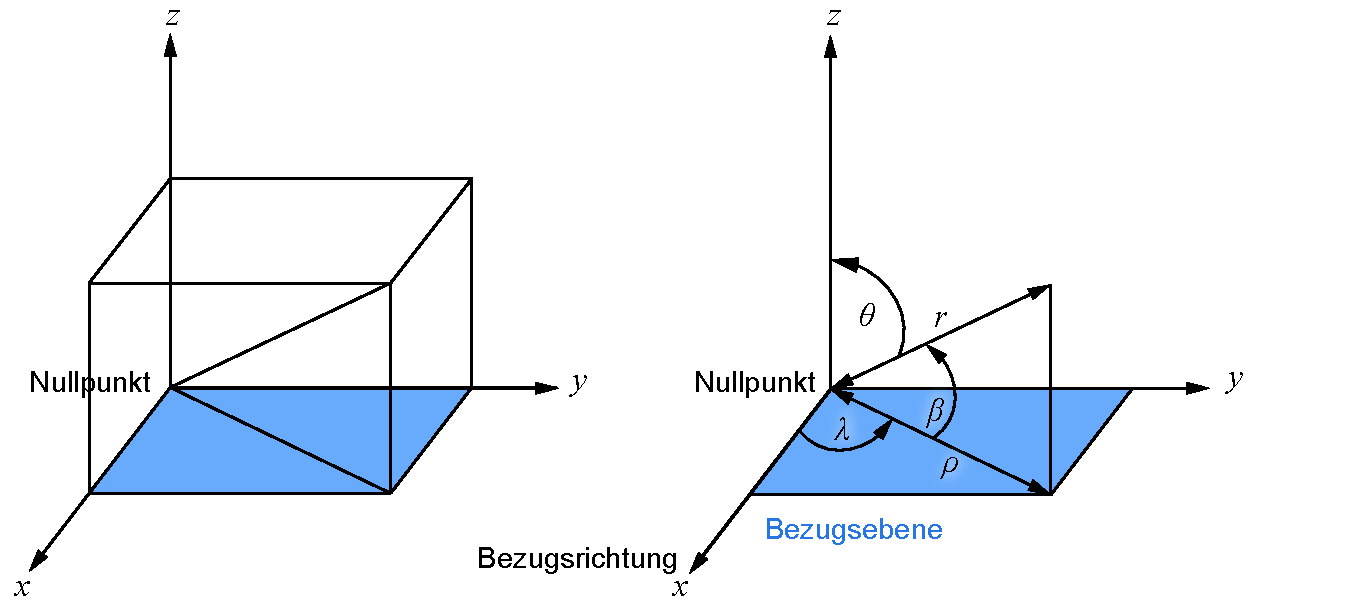
\includegraphics[width=\textwidth]{Koordinatensysteme.pdf}%
\caption[Koordinatensysteme in kartesischen und sph�rischen Polarkoordinaten.]{Koordinatensysteme in kartesischen und (astronomischen) sph�rischen Polarkoordinaten. Gegen�ber dem mathematischen sph�rischen KOS nutzt man im astronomischen sph�rischen KOS den Winkel $\beta = 90\degree -\theta$.}%
\label{abb:hm_koordinatensysteme}%
\end{figure}
Die Umrechnung zwischen den beiden Koordinatensystemen ist gegeben durch
\begin{align*}
x &= r\,\cos\beta\,\cos\lambda ~,\\
y &= r\,\cos\beta\,\sin\lambda ~,\\ 
z &= r\,\sin\beta ~.\\ 
\smallskip
r &= \sqrt{\rho^2 + z^2} &&\text{ mit } \rho=\sqrt{x^2+y^2} \,,  \nonumber\\
\beta &= \arctan(z/\rho) &&\text{ f�r } \rho\neq 0 \text{; ansonsten 0\textdegree, 90\textdegree\ oder -90\textdegree\ je nach Quadrant.} \nonumber\\
\psi &= 2\arctan\lk \frac{y}{\abs{x}+\rho} \rk\,, \nonumber\\
\lambda &= \psi &&\text{f�r } x=0 \text{ und } y>0 \text{ (auf der positiven $y$-Achse)} \,,\nonumber\\
\lambda &= \psi &&\text{f�r } x>0 \text{ und } y\geq 0 \text{ (1. Quadrant)} \,, \nonumber\\
\lambda &= 360\text{\textdegree}+\psi &&\text{f�r } x\geq 0 \text{ und } y<0 \text{ (4. Quadrant)} \,,\nonumber\\
\lambda &= 180\text{\textdegree}-\psi &&\text{f�r } x<0 \text{ (2. und 3. Quadrant)} \,,\nonumber\\
\lambda &= 0\text{\textdegree} &&\text{f�r } x=0 \text{ und } y=0 \text{ (im Ursprung)} ~~. \nonumber
\end{align*}
Bei der Berechnung der arctan-Funktionen muss man etwas aufpassen und sich �berlegen, in welchem Quadranten der Winkel liegt.
In \matlab{} ist dazu die Funktion atan2 hinterlegt, die \iw der hier angegebenen Berechnung f�r $\psi$ entspricht und vor allem bei ganzzahligen Vielfachen von $\pi$ f�r $\psi$ genauere Werte liefert.
Die Formel l�sst sich leicht �ber die Beziehung f�r den Tangens des halben Winkels herleiten. Dazu formt man diese �ber
	\[
	\tan\lk \frac{\psi}{2} \rk= \frac{-x \pm \sqrt{x^2+y^2}}{y} = \cot \lk\frac{\psi}{2}-90\degree \rk
\]
um und stellt dann die entsprechenden Fallunterscheidungen f�r $x$ und $y$ an.

F�r die Himmelsmechanik empfehlen sich nun zur Festlegung eines KOS zwei nat�rlich \anf{ausgezeichnete} Bezugsebenen:
\begin{itemize}
\item Die Bahnebene\index{Bahnebene}\footnote{Wir haben ja bereits im Kapitel 1 von Band I gezeigt, dass die Bewegung eines K�rpers im Zentralkraftfeld wegen der Drehimpulserhaltung in einer Ebene stattfindet.  
Wir k�nnen deshalb die Bewegung in einer Bahnebene als gesichert annehmen. In \kapitel{hm_bewegungsgl} werden wir das noch einmal detailliert zeigen.} der Erde um die Sonne (\emph{\gls{ekliptik}}).
\item Die Ebene, die durch den Erdmittelpunkt geht und senkrecht zur Erdachse liegt (\emph{�quatorebene} \index{Aequator@�quator}).
\end{itemize}
Die Schnittlinie zwischen der Ekliptik und der �quatorebene ergibt dann eine besonders ausgezeichnete gemeinsame Bezugsrichtung/Bezugslinie.
Schaut man auf dieser Bezugslinie (\figref{hm_ekliptik-aequator}) von der Erde in Richtung zur Sonne, dann wird der Schnittpunkt der Erdbahn, wenn diese die Bezugslinie in der Richtung vom Himmelss�dpol zum Himmelsnordpol\footnote{Als Himmelspole\index{Himmelspol} werden die Durchsto�punkte der Erdachse mit der gedachten Himmelskugel bezeichnet.} schneidet, \emph{\gls{fruehlingspunkt}} $\vernal$ genannt.\footnote{Im geozentrischen Bild, das wir gleich noch erl�utern werden, kann man den Fr�hlingspunkt\index{Fr�hlingspunkt|textbf} auch als Schnittpunkt der Sonnenbahn mit dem Himmels�quator auf der gedachten Himmelskugel betrachten (wiederum in der Richtung von S�d nach Nord).} 
Die beiden Ebenen (Ekliptik, �quator) und die Richtung von Erde zum Fr�hlingspunkt dienen somit als Grundlage f�r verschiedene astronomische Koordinatensysteme.
Als Nullpunkt kann der Beobachtungsort entweder im Sonnen- (heliozentrisch\index{Koordinatensystem!heliozentrisches}) oder Erdmittelpunkt (geozentrisch\glslink{geozentrkoord}) gew�hlt werden -- beides keine besonders komfortablen, daf�r aber mathematisch sehr vorteilhafte Beobachtungspunkte.\footnote{An dieser Stelle sei noch einmal auf die grunds�tzliche Raum-Zeit-Problematik in der Himmelsmechanik hingewiesen: Weder der �quator (\bzw die Polachse der Erde) noch die Ekliptik sind wirklich fest im Raum, sondern sie werden durch Kr�fte der verschiedenen Himmelsk�rper in ihrer Lage ver�ndert. Deshalb muss zu jeder Angabe von Koordinaten in einem bestimmten Koordinatensystem eine Zeitangabe gemacht werden.} 
\begin{figure}%
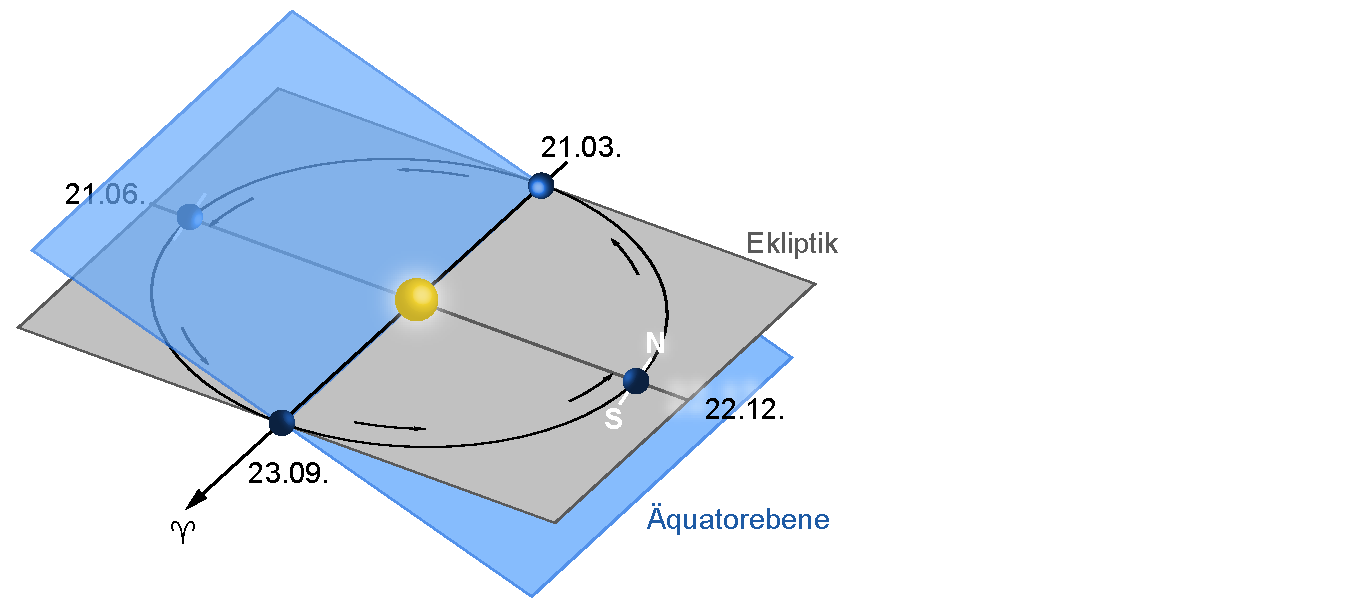
\includegraphics[width=\textwidth]{EkliptikAequator.pdf}%
\caption{Ekliptik, �quator und Fr�hlingspunkt.}%
\label{abb:hm_ekliptik-aequator}%
\end{figure}

Weitere ausgezeichnete Bezugsebenen sind die Bahnebene eines Himmelsk�rpers und die Horizontebene\index{Horizontebene} eines Beobachters auf der Erdoberfl�che: Beide sind f�r Beobachtungsdaten sehr wichtig.
Die Wahl von Bezugsebene, Bezugsrichtung ($x$-Achse) und Nullpunkt (Ursprung) ergeben die verschiedenen Koordinatensysteme, die wir in Tabelle \ref{tab:hm_astro_KOS} zusammengefasst haben.
F�r eine tiefergehende Darstellung der verschiedenen Koordinatensysteme empfehlen wir die Darstellungen in \cite{Montenbruck1999,Praxl2016,Meeus1998}. \\
Wir geben in \figref{hm_geozent_KOS} die graphische Darstellung des geozentrisch-ekliptikalen KOS\index{Koordinatensystem!geozentrisch-ekliptikales} (GE) und des geozentrisch-�quatorialen KOS\index{Koordinatensystem!geozentrisch-�quatoriales} (GA) an.
Letzteres rotiert mit dem Fixsternhimmel mit, ist also fest mit diesem verbunden und wird deswegen auch \emph{space-fixed} GA-KOS genannt (GA(sf)).
Die Definition der zum jeweiligen System geh�renden Koordinaten ist in \figref{hm_geozent_KOS} ersichtlich und im Detail in Tabelle \ref{tab:hm_astro_KOS} aufgef�hrt.

\begin{figure}%
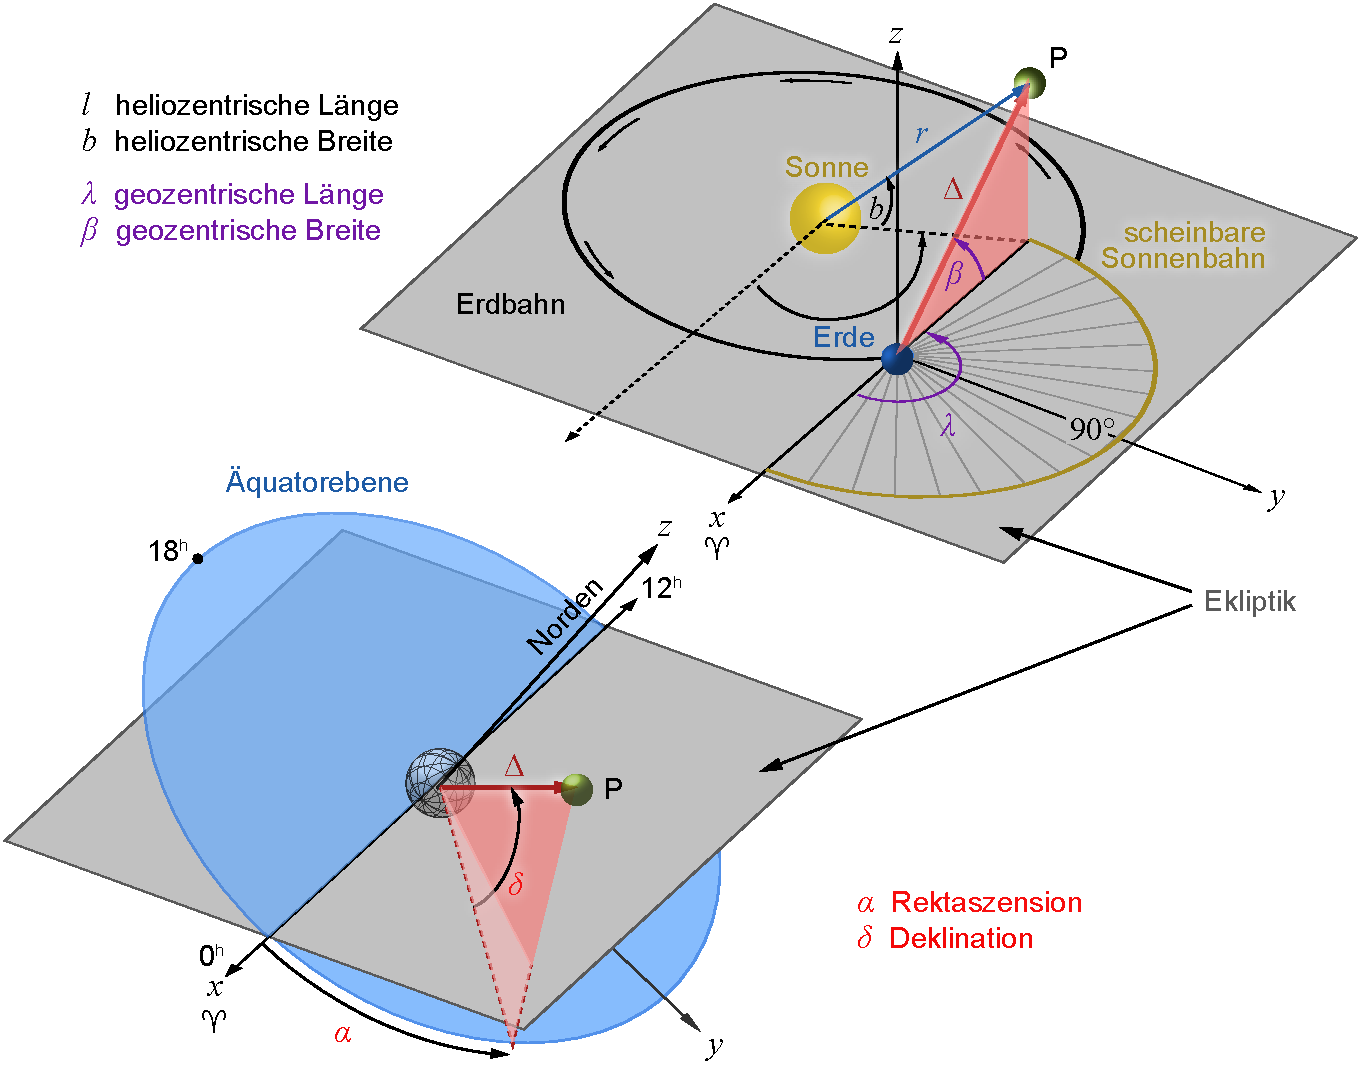
\includegraphics[width=\textwidth]{GE_und_GAe_KOS.pdf}%
\caption[Geozentrisch-ekliptikales und geozentrisch-�quatoriales KOS]{Geozentrisch-ekliptikales und geozentrisch-�quatoriales KOS. Die einzelnen Parameter und ihre Beziehungen zueinander sind im Detail in Tabelle \ref{tab:hm_astro_KOS} erl�utert.}%
\label{abb:hm_geozent_KOS}%
\end{figure}

Die Umrechnungen zwischen den einzelnen KOS haben wir in Tabelle \ref{tab:hm_Umrechung_KOS} im Tabellenanhang angegeben.
Die Herleitung kann �ber die Formeln der sph�rischen Trigonometrie \cite{Smart1986} oder eleganter �ber Rotations- bzw. Drehmatrizen\index{Rotationsmatrix} \index{Drehmatrix} (siehe Kap. 1.2 in Band I \bzw \cite{Montenbruck1999}) erfolgen, da die Transformationen zwischen den einzelnen Koordinatensystemen jeweils durch Drehungen und/oder Translationen beschrieben werden k�nnen.
Wir wollen das am Beispiel der Transformation des Ortsvektors $\vec{r}$ im geozentrisch-ekliptikalen KOS (GE) in den Ortsvektor $\vec{r}'$ des geozentrisch-�quatorialen KOS (GA(sf)) demonstrieren.
Diese Transformation entspricht, wie wir aus \figref{hm_geozent_KOS} erkennen, einer Drehung um die $x$-Achse um die \emph{Schiefe der Ekliptik}\index{Schiefe der Ekliptik} $\epsilon$.
Der Winkel $\epsilon$ ist identisch zur Neigung der Erdachse\index{Neigung Erdachse} gegen ihre Bahnebene.
Die entsprechende Drehung wird durch folgende Matrizen beschrieben:
\begin{align}
\begin{split}
\vec{r}' &= \mathbb{R}_x(-\epsilon)\cdot \vec{r} = \lk \begin{array}{ccc} 1 & 0 & 0 \\ 0 & \cos\epsilon & -\sin\epsilon \\ 0 & \sin\epsilon & \cos\epsilon \end{array}\rk \lk \begin{array}{c} x \\ y\\ z \end{array}\rk ~,~~~\vec{r}' = \lk \begin{array}{c} r\cos\delta\cos\alpha \\ r\cos\delta\sin\alpha \\ r\sin\delta \end{array}\rk\,,\\
\vec{r} &= \mathbb{R}_x(\epsilon)\cdot \vec{r}' = \lk \begin{array}{ccc} 1 & 0 & 0 \\ 0 & \cos\epsilon & \sin\epsilon \\ 0 & -\sin\epsilon & \cos\epsilon \end{array}\rk \lk \begin{array}{c} x' \\ y' \\ z' \end{array}\rk \,, ~~~ \vec{r} = \lk \begin{array}{c} r\cos\beta\cos\lambda \\ r\cos\beta\sin\lambda \\ r\sin\beta \end{array}\rk \,.
\end{split} \label{eq:hm_drehung_x_achse1}
\end{align}

\begin{sidewaystable}
\vspace{12cm}
\caption{Astronomische Koordinatensysteme und deren Parameter.}
\begin{tabular}{L{1cm}|L{3.5cm}|L{2cm}|L{2cm}|L{2cm}|L{2cm}|L{3cm}l}
\hline\noalign{\smallskip}
Kurz-		& Bezeichnung &	Ursprung  & Bezugs- & Bezugsrichtung  &	Vertikale  & Horizontale &	Koordinaten \\
zeichen &							&						& ebene		& $x$-Achse				& Koordinaten	& Koordinaten &							\\
\noalign{\smallskip}\svhline\noalign{\smallskip}
\multicolumn{8}{l}{Absolute Systeme}	\\					
\noalign{\smallskip}\svhline\noalign{\smallskip}	
BA & Bahnkoordinaten & Zentralk�rper & Bahn & \gls{periapsis} & - &	Abstand $r$, \linebreak Anomalie $\upsilon$  & $\lk \begin{array}{c} r\,\cos \upsilon \\r\,\sin \upsilon \\ 0 \end{array}\rk$ \\
BA & Bahnkoordinaten & Zentralk�rper & Bahn & Knoten\index{Knoten} & - &	Abstand $r$,\linebreak Winkel $u\!=\!\upsilon\!+\!\omega$,\linebreak L�nge der Periapsis $\omega$ & $\lk \begin{array}{c} r\,\cos u \\r\,\sin u \\ 0 \end{array}\rk$\\
HE & Heliozentrisch-ekliptikal & Sonne (Mittelpunkt) & Ekliptik & $\vernal$ & Ekliptikale Breite $b$ & Ekliptikale L�nge $l$ & $\lk \begin{array}{c} r\,\cos b\,\cos l \\ r\,\cos b\,\sin l \\ r\,\sin b \end{array}\rk$\\
GE & Geozentrisch-ekliptikal & Erde (Mittelpunkt) & Ekliptik & $\vernal$ & Ekliptikale Breite $\beta$ & Ekliptikale L�nge $\lambda$	& $\lk \begin{array}{c} \Delta\,\cos \beta\,\cos \lambda \\ \Delta\,\cos \beta \,\sin \lambda \\ \Delta\,\sin \beta \end{array}\rk$\\
GA(sf) & Geozentrisch-�quatorial (space-fixed) & Erde (Mittelpunkt) & �quator & $\vernal$ & \gls{dekl} $\delta$ & \gls{rektasz} $\alpha$ & $\lk \begin{array}{c} \Delta\,\cos \delta\,\cos \alpha \\ \Delta\,\cos \delta\,\sin \alpha \\ \Delta\,\sin \delta \end{array}\rk$\\
\noalign{\smallskip}\svhline\noalign{\smallskip}
\multicolumn{8}{l}{Relative Systeme}	\\					
\noalign{\smallskip}\svhline\noalign{\smallskip}	
GA(ef) & Geozentrisch-�quatorial (earth-fixed) & Erde (Mittelpunkt) & �quator & Meridian (Greenwich) & Deklination $\delta$ & Stundenwinkel $\tau$ & $\lk \begin{array}{c} \Delta\,\cos \delta\,\cos \tau \\ \Delta\,\cos \delta\,\sin \tau \\ \Delta\,\sin \delta \end{array}\rk$\\
TA & Topozentrisch-�quatorial & Topozentrum (Beobachter) & Parallele \linebreak (zum �quator) & Meridian (Greenwich) & Deklination $\delta'$ & Stundenwinkel $\tau$ & $\lk \begin{array}{c} \Delta'\,\cos \delta' \,\cos \tau \\ \Delta'\,\cos \delta'\,\sin \tau \\ \Delta'\,\sin \delta' \end{array}\rk$\\
TH & Topozentrisch-horizontal & Topozentrum (Beobachter) & Horizont & S�den (Meridian) \linebreak Beobachter & H�henwinkel $h$ & Azimut $\mathcal{A}$ & - \\
\noalign{\smallskip}\hline\noalign{\smallskip}
\end{tabular}
\label{tab:hm_astro_KOS}
\end{sidewaystable}


Daraus ergeben sich dann folgende Umrechnungsformeln f�r GE nach GA(sf):
\begin{align}
\cos\delta\cos\alpha &= \cos\beta\cos\lambda  \,, \label{eq:hm_drehung_x_achse_linear2} \\
\cos\delta\sin\alpha &= \cos\beta\sin\lambda\cos\epsilon - \sin\beta\sin\epsilon \nonumber \,,\\
\sin\delta &= \cos\beta\sin\lambda\sin\epsilon + \sin\beta\cos\epsilon  \nonumber ~~.
\end{align}
In umgekehrter Richtung von GA(sf) nach GE gilt dann:
\begin{align}
\cos\beta\cos\lambda &= \cos\delta\cos\alpha \,,\label{eq:hm_drehung_x_achse_linear_3} \\ 
\cos\beta\sin\lambda &= \cos\delta\sin\alpha\cos\epsilon + \sin\delta\sin\epsilon \nonumber \,,\\
\sin\beta &= \sin\delta\cos\epsilon - \cos\delta\sin\alpha\sin\epsilon  \nonumber ~~.
\end{align}
In \probref{hm_trafo_koord} werden die Dreh- und Translationsmatrizen f�r die in Tabelle \ref{tab:hm_Umrechung_KOS} im Tabellenanhang aufgef�hrten KOS-Transformationen verifiziert. \\
Im Gegensatz zu den beiden gerade besprochenen absoluten Koordinatensystemen\index{Koordinatensystemen!absolutes} sind das geozentrisch-�quatoriale (\emph{earth-fixed}) KOS (GA(ef)) ebenso wie das topozentrisch-horizontale KOS\index{Koordinatensystem!horizontales} (TH) wegen der Erdrotation von der Zeit abh�ngig und geh�ren damit zur Gruppe der relativen KOS.
F�r die Umrechnung zwischen dem raum-fixierten geozentrisch-�quatorialen System\index{Koordinatensystem!geozentrisch-�quatoriales} (GA(sf)) und dem erd-fixierten geozentrisch-�quatorialen System (GA(ef)) f�hrt man den \gls{stundenwinkel} $\tau$ ein.
\gls{rektasz} $\alpha$ und Stundenwinkel $\tau$ sind die einander entsprechenden Koordinaten im GA(sf) bzw. GA(ef)-Koordinatensystem.
Die Rektaszension\index{Rektaszension} ist definiert als Winkel entlang des �quators zwischen der Richtung zum Fr�hlingspunkt\index{Fr�hlingspunkt} $\vernal$ (Bezugsrichtung der Rektaszension) und der Richtung zum Himmelsobjekt (\figref{hm_geozent_KOS} und Tabelle \ref{tab:hm_astro_KOS}).
Die Bezugsrichtung f�r den Stundenwinkel\index{Stundenwinkel} hingegen ist der ortsfeste \gls{meridian} (die S�drichtung).
Der Stundenwinkel eines betrachteten Himmelsk�rpers gibt damit die Differenz zwischen der Rektaszension $\alpha$ dieses K�rpers und der Rektaszension derjenigen Himmelsk�rper an, die gerade ihre gr��te H�he �ber dem Horizont im Meridian erreichen.
Der Stundenwinkel gibt also die Zeit an, die ein Himmelsk�rper noch bis zu seiner \gls{kulmination} braucht bzw. die seit seiner \gls{kulmination} schon verstrichen ist.\footnote{Der Stundenwinkel ist ein Winkel- und Zeitma�. Wir werden in \kapitel{hm_zeitdefinition} den wichtigen Zusammenhang zwischen dem Stundenwinkel und der dort definierten Sternzeit ableiten.} 

\begin{figure}%
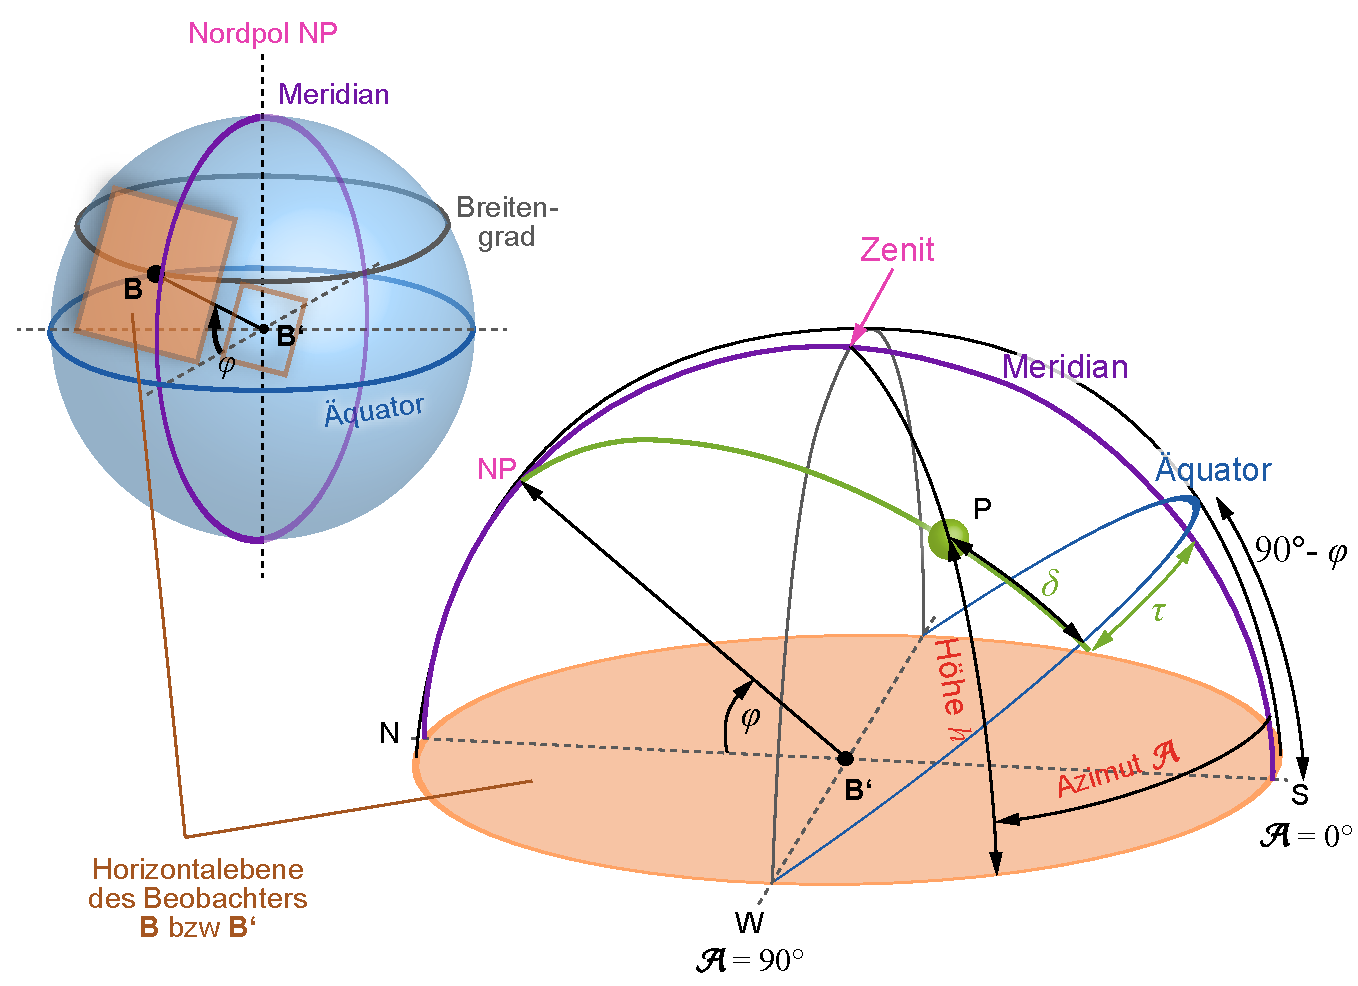
\includegraphics[width=\textwidth]{TH01.pdf}%
\caption{Topozentrisches Horizontalkoordinatensystem.}%
\label{abb:hm_topozent_KOS}%
\end{figure}

Wir betrachten nun noch das topozentrisch-horizontale KOS\index{Koordinatensystem!topozentrisches} (TH) (\figref{hm_topozent_KOS}) etwas genauer.
Dieses stellt f�r den Beobachter auf der Erde das nat�rlichste KOS dar und ist \zb f�r die Berechnung von Aufgangs- und Kulminationszeiten das geeignete Bezugssystem.
Das topozentrisch-horizontale KOS geht offensichtlich durch Drehung um die $y$-Achse um den Winkel $90$\textdegree$-\varphi$ aus dem �quatorialen KOS hervor.\footnote{Die von der Erdoberfl�che aus gemessenen Horizontal- und Vertikalkoordinaten $\alpha',\delta'$ im TA-KOS weichen im Allgemeinen wenig von den gemessenen im GA-KOS $\alpha,\,\delta$ ab.
Ausnahmen sind die Beobachtungen von erdnahen Objekten wie \zb Satelliten, Monden, Kometen und benachbarten Planeten.} Der Beobachter B im topozentrisch-horizontalen KOS befindet sich an einem Ort der \emph{\glslink{geogrkoord}{geographischen Breite}} $\varphi$.
F�r ihn ist dann der jeweilige Himmelspol unter dem Winkel $\varphi$ zu sehen.
Der rechte Teil der \figref{hm_topozent_KOS} zeigt dies f�r die Nordhalbkugel.
Als Meridian\index{Meridian} wird der Gro�kreis an der Himmelskugel bezeichnet, auf dem S�dpunkt und Nordpunkt am Horizont, der \gls{zenit} und die beiden Himmelspole liegen.
Eine h�ufig benutzte Beziehung zwischen dem �quatorialen KOS und dem topozentrisch-horizontalen KOS ist die Berechnung von H�he und \gls{azimut} eines Himmelsk�rpers aus bekannter Deklination und bekanntem Stundenwinkel.
Diese Beziehung l�sst sich wiederum mit Hilfe der Matrizentransformation f�r die Umrechnung der KOS ableiten (Tabelle \ref{tab:hm_Umrechung_KOS}, \probref{hm_trafo_koord}):
\begin{merksatz}{Umrechnung vom �quatorialen KOS in das topozentrisch-horizontale KOS}
\begin{align}
\begin{split}
\sin h &= \cos\delta\cos\tau\cos\varphi+\sin\delta\sin\varphi \,,\\
\tan \mathcal{A} &= \frac{\cos\delta\sin\tau}{\cos\delta\cos\tau\sin\varphi-\sin\delta\cos\varphi} \,. 
\end{split} \label{eq:hm_Alt-Az-Koord}
\end{align}

\end{merksatz}
Wir haben bereits darauf hingewiesen, dass die Bezugsebenen und Bezugsrichtungen der genannten KOS nicht fest im Raum liegen.
Vielmehr f�hren diese durch Kr�fte von anderen Himmelsk�rpern als (astronomische) Pr�zession\index{Pr�zession} bekannte Kreiselbewegungen aus, die wir bereits in Kapitel 1.5.5 im Band I mit einer Modellrechnung untersucht hatten und die in den Referenzen \cite{Montenbruck1999, Murray2008} detailliert beschrieben wird.
So verschiebt sich der Fr�hlingspunkt pro Jahr um etwa 50 Bogensekunden in westlicher Richtung entlang der Ekliptik.
Dieser Effekt ist so gro�, dass er bereits �ber relativ kurze Beobachtungszeitr�ume von einigen Jahren auff�llt.
Damit verschieben sich auch die Nullpunkte der astronomischen Koordinatensysteme langsam entlang der Ekliptik und die ekliptikale L�nge eines Sterns ohne Eigenbewegung nimmt in einem Jahr um \ca 50 Bogensekunden zu.
Die Koordinaten eines Himmelsobjekts �ndern sich also, ohne dass dies einer eigentlichen Bewegung des Objekts entspricht.\footnote{Der Pr�zessionsbewegung �berlagern sich noch zus�tzliche periodische Schwankungen. Diese verschiedenen periodischen Bewegungen, welche die Erdachse zus�tzlich zur Pr�zession ausf�hrt, werden in der Astronomie unter dem Begriff der Nutation\index{Nutation} zusammengefasst. Die Ursachen sind nicht vollst�ndig identisch mit der im Kapitel 1, Band I hergeleiteten Nutation eines schweren Kreisels, aber die Bewegungsform ist sehr �hnlich. Die Verschiebung der �quinoktialpunkte\index{Aequinoktialpunkte@�quinoktialpunkte} entlang der Ekliptik erfolgt also nicht v�llig gleichm��ig, sondern mit periodisch leicht schwankender Geschwindigkeit.}
Deshalb braucht es zur Angabe von Koordinaten von Himmelsk�rpern auch stets den Zeitpunkt, auf den sich die Koordinaten beziehen.
Von besonderer Bedeutung f�r Beobachtungen sind die Koordinaten f�r das �quinoktium des Beobachtungszeitpunkts, das sogenannte \emph{�quinoktium des Datums}\glslink{aequinox}.
Der Begriff \emph{�quinoktium} \index{Aequinoktium@�quinoktium} bezeichnet hier den tats�chlichen, aktuellen Schnittpunkt des Himmels�quators mit der Ekliptik zum Beobachtungszeitpunkt.
Mit \emph{\gls{epoche}}\index{Epoche} wird in der Himmelsmechanik der Zeitpunkt einer Beobachtung bezeichnet.\footnote{Merkregel: Die Epoche bezeichnet den tats�chlichen Zeitpunkt einer Beobachtung oder eines Vorgangs, das �quinoktium das Koordinatensystem, in dem gemessen wird.} Vielfach werden Koordinaten auf Koordinatensysteme sogenannter Stan\-dard\-�qui\-noktien\index{Standard�quinoktium} bezogen, die sich auf bestimmte feste Zeitpunkte (etwas verwirrend auch \emph{Standardepochen}\index{Standardepoche} genannt) beziehen.
\emph{�quinoktium und Epoche J2000} bedeuten \zb dass sich die Koordinatensysteme, Bahnparameter und die Ekliptikschiefe\index{Ekliptikschiefe} $\epsilon$ auf die Lage von �quator, Ekliptik und Fr�hlingspunkt zum 01.\,01.\,2000 beziehen und dass am 01.\,01.\,2000 beobachtet wurde.
F�r diese Epoche gilt beispielsweise $\epsilon\!=\!23.4392911$\text{\textdegree}.
Wir werden im Folgenden f�r die Berechnung von Beobachtungsdaten von Himmelsk�rpern, falls nicht anders angegeben, das �quinoktium dieses Datums benutzen. 

\begin{figure}%
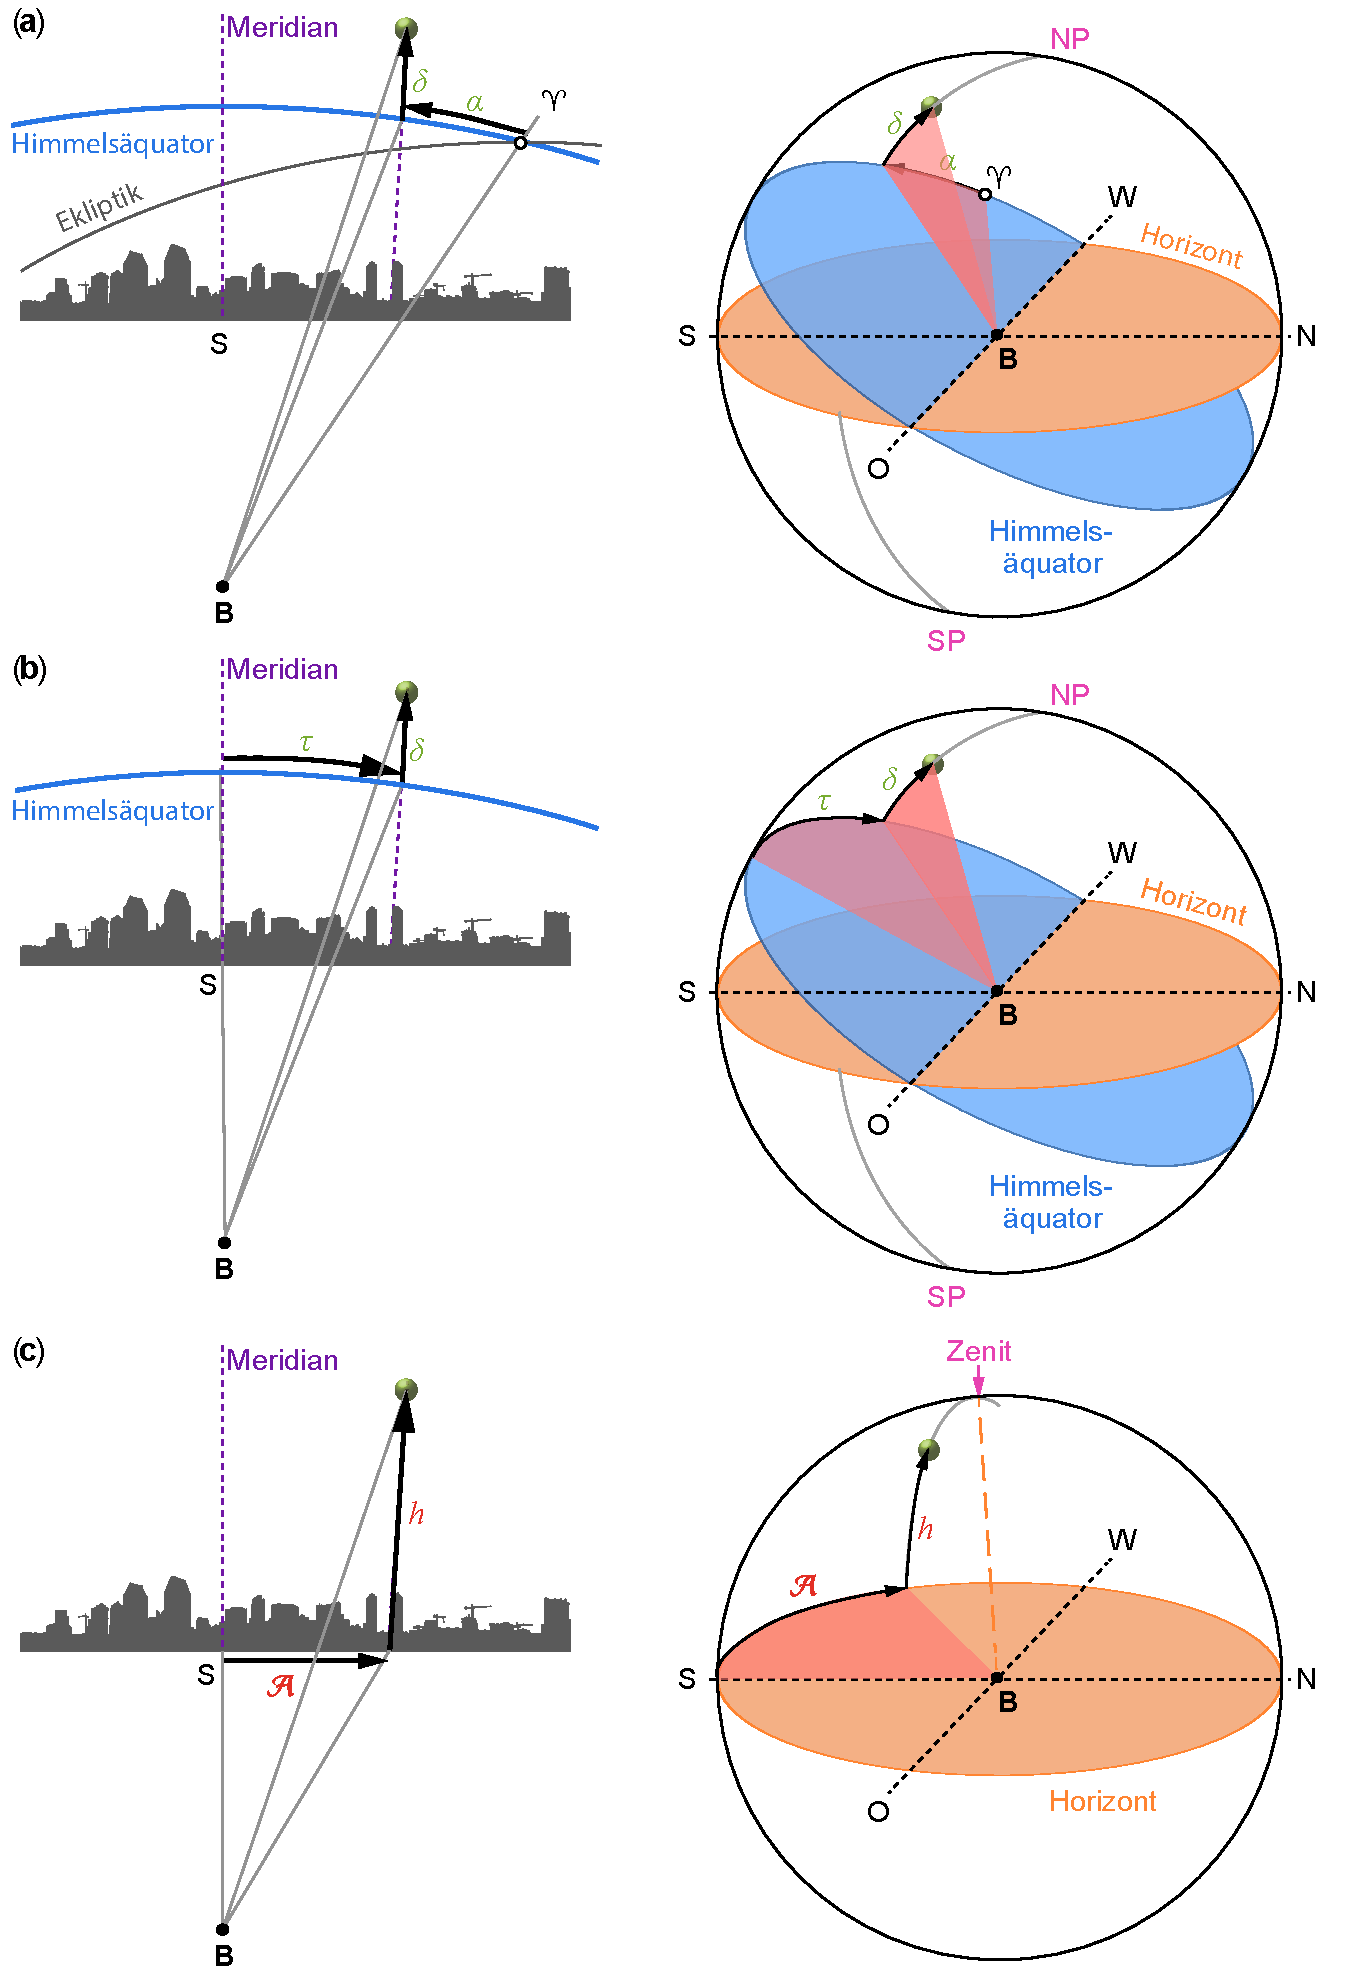
\includegraphics[width=\textwidth]{KOS_Vgl.pdf}%
\caption[Zusammenh�nge zwischen h�ufig benutzten Koordinatensystemen.]{Zusammenh�nge zwischen h�ufig benutzten Koordinatensystemen. \fa Raum-fixiertes geozentrisch"=�quatoriales KOS (GA(sf)), \fb Erd-fixiertes geozentrisch-�quatorales KOS (GA(ef)), \fc Topozentrisch-horizontales KOS (TH).}%
\label{abb:hm_KOS_Abh}%
\end{figure}
\figref{hm_KOS_Abh} fasst noch einmal schematisch die Zusammenh�nge zwischen den verschiedenen gebr�uchlichen KOS zusammen.
Wir wollen uns nun im n�chsten Kapitel etwas n�her mit dem Aspekt der Zeit besch�ftigen.

\subsection{Zeitdefinition}\label{kap:hm_zeitdefinition}
Zeit beschreibt die Abfolge von Ereignissen, hat also eine eindeutige, unumkehrbare Richtung.
Sie wird in ihrer Skala durch wiederkehrende, periodische Vorg�nge definiert, wie sie auch in der Himmelsbeobachtung gegeben sind.
Wir stellen zun�chst die in der Astronomie �bliche \glslink{jd}{Julianische Tagesz�hlung}\index{Julianisches Datum} (\emph{Julian Date}\footnote{Das Julianische Datum wurde 1582 vom Franzosen Joseph Justus Scaliger (1540--1609) eingef�hrt. Nach einer nicht gesicherten Darstellung w�hlte er die Bezeichnung, um damit seinen Vater Julius Scaliger zu ehren und nicht, wie h�ufig vermutet, Julius Caesar.} JD) vor, bei der die Tage fortlaufend seit dem 01.\,01.\,($-$4712) (entspricht dem 01.\,01.\,4713 v. Chr.) durchgez�hlt werden.
Ein neuer Tag im JD beginnt jeweils um 12:00 am Mittag.\footnote{Dank dieser Konvention braucht bei astronomischen Beobachtungen w�hrend der Nacht kein \anf{Datumswechsel} vollzogen zu werden.} So entspricht dem 01.\,01.\,2020 0:00 UT (Mitternacht in Greenwich\footnote{Wir verwenden hier schon die sogenannte Universal Time UT, die wir erst sp�ter genauer definieren. Vorerst gen�gt die Annahme, dass wir eine Uhr haben, die wir UT nennen, auf der unsere astronomische Zeitz�hlung beruht.}) das Julianische Datum J\,2458849.5,
dem 01.\,01.\,2021 das Julianische Datum\index{Julianische Datum} J\,2459215.5, dazwischen liegen demzufolge $\text{J\,}2458849.5 - \text{J\,}2459215.5\!=\!366\,\text{Tage}$, denn 2020 war ein Schaltjahr.
H�ufig wird auch das \emph{Modifizierte Julianische Datum} MJD\index{Datum!Modifiziertes Julianisches} verwendet, welches als $\text{MJD}\!=\!\text{JD\,}-2400000.5$ definiert wird.
Ferner sei noch angemerkt, dass ein nach dem JD berechnetes Julianisches Jahrhundert immer ganzzahlige $36525$ Tage hat, die man in exakt $24$ Stunden zu $3600$ Sekunden unterteilt.
Es gibt in Computerprogrammen (so auch in \matlab) hinterlegte Routinen zur Berechnung des JD aus dem Kalenderdatum und umgekehrt \cite{Praxl2016,Meeus1998}.
Mit dem Julianischen Datum haben wir eine elegante Z�hlung beschrieben, mit der wir in der Himmelsmechanik sowohl gro�e als auch kleine Zeitr�ume, wie \zb Tagesabschnitte, einheitlich beschreiben k�nnen. 
Wir m�ssen aber neben der durch das JD definierten Z�hlweise auch die zugrundeliegende Zeit physikalisch definieren.
Es sind verschiedene Zeitdefinitionen m�glich, und wir unterscheiden (siehe auch \cite{McCarthy2018}):
\begin{itemize}
    \item durch Bewegungsgesetze definierte \emph{dynamische} Zeitskalen (\zb Ephemeridenzeit\footnote{Als \emph{\gls{ephemeride}}\index{Ephemeride} wird ganz allgemein die Positionsangabe eines Himmelsk�rpers bezogen auf ein bestimmtes KOS bezeichnet. Himmelsmechanik ist also nichts anderes als die Bestimmung der Ephemeriden als Funktion der Zeit.} ET),
    \item Realisierungen durch eine absolut \emph{gleichm��ig ablaufende} Zeit (Atomzeit TAI),
    \item die b�rgerliche oder \emph{Alltagszeit} (Universal Time UT, Universal Time Coordinated UTC) und
    \item \emph{erdrotationsabh�ngige} Zeitskalen (Wahre Sonnenzeit und Sternzeit).
\end{itemize}

\subparagraph{Dynamische Zeit:}
F�r die Berechnungen in der Himmelsmechanik ben�tigen wir die dynamische Zeit.
Das ist die Zeit, die auch in den zeitlichen Ableitungen der Bewegungsgleichungen \anf{steckt}.
Sinnvollerweise benutzt man zur Zeitma�definition periodische Bewegungen der Himmelsk�rper.
Die Umlaufdauer\index{Umlaufzeit} der Erde um die Sonne ist weitgehend konstant, und man definiert daher den zeitlichen Abstand zwischen zwei Durchg�ngen durch den Fr�hlingspunkt $\vernal$ als \emph{tropisches Jahr}\glslink{tropischesjahr}.
Die Internationale Astronomische Union hat 1960 daraus die sogenannte \index{Ephemeridenzeit} \emph{Ephemeridenzeit} ET \glslink{et} (engl.\ \emph{ephemeris time}) �ber die Festlegung der Ephemeridensekunde als SI-Einheit\footnote{Sp�ter wurden auf Basis von anderen und verbesserten Messmethoden geringf�gig von ET \anf{abweichende} dynamische Zeiten eingef�hrt (\zb TT, TDT).
F�r unsere Zwecke spielen die Unterschiede keine Rolle.
Wir benutzen deshalb die Ausdr�cke Ephemeridenzeit (ET) und dynamische Zeit (TT, TDT) synonym.} definiert: Eine Ephemeridensekunde ist der Bruchteil 1/31556925.9747 des tropischen Jahres.
Daraus ergibt sich mit der L�nge eines Tages (Ephemeridentag) von genau $86400$ Ephemeridensekunden ($1\,\text{d}= 86400\,\text{s} = 24 \cdot 60 \cdot 60\:\text{s}$) die L�nge eines tropischen Jahres in Tagen (d) zu
\begin{align*}
a_\text{trop} = 365.2421988\,\text{d}\,. 
\end{align*}
Die Nachkommastellen von $a_\text{trop}$ sind den Astronomen seit dem Altertum gut bekannt und haben im Laufe der Zeit zur Einf�hrung verschiedener Kalendersysteme und Schaltjahresfestlegungen gef�hrt.

\subparagraph{Gleichm��ig ablaufendes Zeitma� (Atomzeit):}
Die Ephemeridensekunde wurde als SI-Einheit bereits 1967 durch die Sekundendefinition �ber die \emph{Atomzeit} TAI \glslink{tai} (\emph{Temps Atomique International}) abgel�st.
Die Atomzeit ist die derzeit beste Realisierung einer dynamischen Zeit.
Deren Definition wurde aber so gew�hlt, dass sie im Rahmen der Messgenauigkeit mit der Ephemeridensekunde �bereinstimmt.
F�r praktische Zwecke kann daher die Ephemeridensekunde als identisch mit der Atomsekunde betrachtet werden.
Zwischen beiden so definierten Zeiten besteht eine nahezu konstante Differenz von
\begin{equation}
\text{ET} - \text{TAI} = 32.184 \text{s} ~.
\label{eq:hm_ET-TAI}
\end{equation}

\subparagraph{B�rgerliche Zeit:}
Unsere normale Uhrzeit im Alltag, die Weltzeit\index{Universal Time} UT\glslink{ut}\ (\emph{Universal Time}) wird vom Mittagsdurchgang der \anf{mittleren} Sonne abgeleitet.
Dies ist aber eine fiktive Sonne, deren scheinbare Bahn eine gleichf�rmig durchlaufene Kreisbahn ist und die mit der wahren Sonne zu bestimmten Zeiten zusammentrifft.
Da diese so definierte Zeit von der Erdrotation abh�ngt, diese sich aber verlangsamt (\probref{hm_erdrotation}) und unregelm��ig ist, wird die UT zunehmend von der gleichm��ig ablaufenden TAI abweichen.
Die UT-Uhr l�uft quasi seit einem Null-Zeitpunkt, an dem die beiden Uhren definitionsgem�� synchronisiert wurden -- das war der 01.01.1900 -- mittlerweile um 
\begin{align*}
\Delta T &= \ET-\UT = (\ET-\TAI) + (\TAI-\UT) = 32.184\:\text{s} + \sum{\text{leaps}}
\end{align*}
der Atomuhr hinterher (und \anf{stottert} auch noch ein bisschen). $\sum{\text{leaps}}$ ist dabei das gemessene Auseinanderlaufen von TAI und UT. Mit der UTC (Universal Time Coordinated) wurde eine Verkn�pfung zwischen UT und TAI hergestellt.
Die UTC weicht dabei nur um ganze Schaltsekunden\index{Schaltsekunde} von TAI und nur um maximal $\SI{0.9}\second$ von UT ab.
UTC, die wir im Alltag verwenden, stellte also durch die Einf�hrung von Schaltsekunden einen Gleichlauf mit der Atomzeit immer wieder her. F�r unsere Rechnungen setzen wir immer $\UT\!\approx\!\UTC$.\footnote{Das in unregelm��igen Abst�nden vorgenommene Einf�gen sorgt f�r eine Menge Anpassungsschwierigkeiten f�r Computer und IT-Systeme. 2012 kam es danach zu Problemen bei Mozilla, LinkedIn und dem Flugbuchungsdienst Amadeus. Eine falsche Schaltsekunde st�rte auch schon Linux-Systeme. Entschieden hat das \textit{Bureau International des Poids et Mesures} (BPIM) jetzt, dass die koordinierte Weltzeit (UTC) zwischen 2035 und 2135 nicht durch Schaltsekunden unterbrochen werden soll. Dann soll ein Maximalwert f�r die erlaubte Differenz gelten und gegebenenfalls etwa eine Schaltminute eingef�gt werden. Die Wissenschaft solle die Zeit bis dahin jetzt nutzen, um eine weniger problematische L�sung zu finden. Der Abschaffung der Schaltsekunde hat die \textbf{International Telecommunication Union} (ITU) final im Dezember 2023 zugestimmt.}.
 Zum 01.\,01.\,2020 waren es bereits $\SI{37}{\second}$.
Die historische Entwicklung von $\Delta T$ wird in\cite{Espenak2014} angegeben.  

Wir wollen an dieser Stelle noch die Konvention festhalten, dass sich, wenn keine weiteren Angaben gemacht werden, das Julianische Datum auf eine Zeitangabe in UT bezieht.
Ben�tigt man ein Julianisches Datum mit einer dynamischen Zeitskala als Referenz, dann muss man dies entsprechend kennzeichnen, \zb mit den Symbolen JE oder J(ET). 

\subparagraph{Erdrotationsabh�ngige Zeitskalen (Wahre Sonnenzeit und Sternzeit):}
Als weitere in der Astronomie gebr�uchliche Zeit wollen wir die \emph{\gls{sternzeit}} $\theta$ behandeln.
Die regelm��ige scheinbare Bewegung des Fixsternhimmels eignet sich ebenfalls gut f�r eine Festlegung einer Zeit.
Die Sternzeit definiert sich aus dem \emph{Sterntag}, welcher der Dauer zwischen zwei Meridiandurchg�ngen des Fr�hlingspunktes $\vernal$ entspricht.\footnote{Da der Fr�hlingspunkt ebenfalls nicht fest im Raum ist, sondern sich wegen der Erdpr�zession pro Tag um etwa $0.137''$ r�ckl�ufig entlang der Ekliptik bewegt, f�llt ein mittlerer Sterntag um $\SI{0.009}{\second}$ k�rzer aus als eine Erdrotation.}

In \kapitel{hm_koordinatensysteme} hatten wir bei der Definition des geozentrisch-�quatorialen KOS GA(ef) den Stundenwinkel $\tau$ eingef�hrt, welcher die Verbindung  der Raumkoordinaten mit der Erdrotation und damit mit der Zeit herstellte.
Die Sternzeit steht nun in einer direkten Beziehung zum Stundenwinkel.
Den Stundenwinkel $\tau$ eines Himmelsobjektes O hatten wir definiert als den entlang des Himmels�quators vom Meridian des Beobachters zum Objekt gemessenen Winkel.
Andererseits ist die Rektaszension $\alpha$ des Objekts O der entlang des �quators gemessene Winkel vom Fr�hlingspunkt $\vernal$ zum Objekt.
Steht dieses Objekt O nun auf dem Meridian des Beobachters, kulminiert also das Objekt, ist der Stundenwinkel $\tau=0$.
Nimmt man den Fr�hlingspunkt $\vernal$ als Objekt, muss an der Position des Beobachters die Sternzeit gem�� Definition gleich dem Stundenwinkel $\tau$ des Fr�hlingspunktes sein: $\theta\!=\!\tau(\,\vernal)$.
Daraus folgt f�r ein beliebiges Objekt O, welches den Stundenwinkel $\tau$ hat, dass die Sternzeit am Ort des Beobachters B gleich der Summe aus Stundenwinkel $\tau$ und Rektaszension $\alpha$ ist, d.\,h.
\begin{equation}
\theta = \tau + \alpha
\label{eq:hm_std_winkel_tau} \,.
\end{equation}

\begin{figure}%
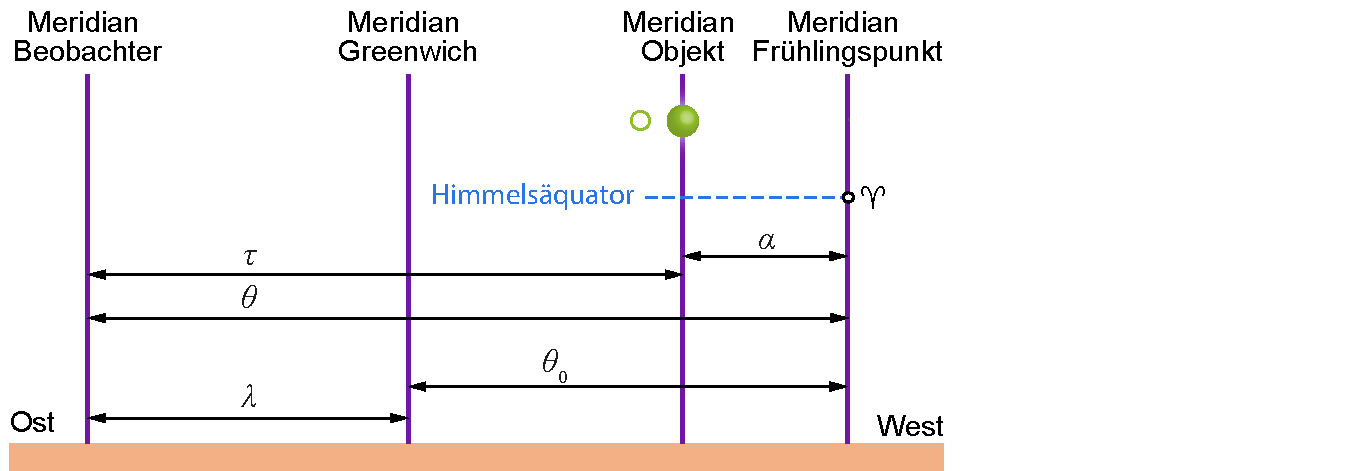
\includegraphics[width=\textwidth]{Vgl_Sternzeit_Tau.pdf}%
\caption[Sternzeit, Rektaszension, Stundenwinkel und geographische L�nge.]{Zusammenhang zwischen Sternzeit, Rektaszension, Stundenwinkel und geographischer L�nge.}%
\label{abb:hm_Sternzeit_Stundenwinkel}%
\end{figure}
Man verdeutliche sich dies anhand von \figref{hm_Sternzeit_Stundenwinkel}.
Die Sternzeit ist f�r alle Beobachter, die sich auf demselben L�ngengrad\index{L�ngengrad} $\lambda$ befinden, gleich gro� und ist damit eine Ortszeit.
Die (mittlere) Sternzeit des Referenzortes Greenwich G ist die Mittlere Greenwich Sternzeit GMST $\theta_0$ (\emph{engl.} Greenwich Mean Sidereal Time)\glslink{gmst}.
Die Ortssternzeit\index{Sternzeit!Orts-} $\theta$ am Beobachterort B wird mit LMST (\emph{engl.} Local Mean Sidereal Time) bezeichnet und berechnet sich mit dem L�ngengrad $\lambda$ (in \textdegree) wie folgt aus der GMST:
\begin{equation}
\text{LMST} = \theta = \text{GMST} + \lambda\,\frac{24 ^\text{h}}{360\degree}  = \theta_0 + \frac{\lambda}{15} \lk \frac{^\text{h}}{\degree} \rk \,. \label{eq:hm_LMST}
\end{equation}
Umgekehrt folgt aus der Differenz der lokalen Sternzeit eines Ortes zur Sternzeit in Greenwich die geographische L�nge dieses Orts.
Eine Messung dieser lokalen Sternzeit, \zb durch Bestimmung der Kulmination eines Sterns mit bekannter Rektaszension, entspricht daher einer geographischen Ortung, wenn die mittlere Greenwich Sternzeit bekannt ist (Beispiel \ref{bsp:laengengrad_abst_fl}).


%BEISPIEL 1 %%%%%%%%%%%%%%%%%%%%%%%%%%%%%%%%%%%%%%%%%%%%%%%%%%%%%%%%%%%%%%%%%%%%%%%%%%%%%%%%%
\begin{example}{Bestimmung von L�ngengrad und Abst�nden auf sph�rischen Fl�chen}  
Es sollen die Unsicherheit der Bestimmung eines L�ngengrades auf See, der Winkelabstand zweier Himmelsk�rper und die k�rzeste Flugstrecke zwischen zwei St�dten auf der Erdoberfl�che berechnet werden.
\begin{enumerate}[(a)]
	\item \emph{Wir wollen die Unsicherheit der Bestimmung eines L�ngengrades auf See nach einer dreimonatigen Seereise unter der Annahme einer perfekten Kulminationsbestimmung eines Sternes und einer Gangungenauigkeit der mitgef�hrten Uhren (auf GMST gestellt) von $1$, $3$, $5\:$s pro Tag berechnen.} \\ 	\medskip 
	Wir bezeichnen die Gangungenauigkeit mit $\Delta g\!=\!1\:\text{s}$, $3\:\text{s}$ \bzw $5\:\text{s}$.
        Die Seefahrt von \ca 3 Monaten dauere n�herungsweise 100 Tage, was eine Uhren-Gesamtverz�gerung von $\Delta g_{\text{tot}}\!=\!100\:\text{s}$, $300\:\text{s}$ bzw. $500\:\text{s}$ gegen�ber einer perfekten (auf Sternzeit \anf{geeichten} Uhr) nach sich zieht.
        Aus \eqref{eq:hm_LMST} folgt durch Differenzenbildung
\begin{equation*}
\Delta\theta = \Delta g_{\text{tot}} = \frac{\Delta\lambda}{15\degree} \,.
\end{equation*}
Hierin sind $\Delta g$ in Stunden anzugeben.
Es folgt:
\begin{equation*}
\Delta\lambda\lek\degree\rek = \frac{15}{3600}\,\Delta g_{\text{tot}}\lek\text{s}\rek = \begin{cases} \ \approx 25' \\ \approx 75' = 1\degree 15' \\ \approx 125' = 2\degree 05' \end{cases}
\end{equation*}
Das sind schon betr�chtliche Abweichungen.
Auf dem �quator sind das im letzten Fall �ber $\SI{200}{\kilo\metre}$.
Das zeigt, vor welchem Problem die nautische Navigation lange Zeit stand.
Dies konnte erst befriedigend mit der Entwicklung hinreichend genauer Uhren durch John Harrison\indexp{Harrison, John} (1693--1776) gel�st werden.
Harrison war ein englischer Erfinder und Uhrmacher.
Seine mechanischen und schiffstauglichen Uhren erm�glichten erstmals pr�zise Zeitmessungen auf See und damit die genaue Bestimmung des L�ngengrades.
Man kann daher auch verstehen, dass lange Zeit versucht wurde, die Zeit \bzw L�ngenbestimmung auf See durch Messung sehr genau bekannter astronomischer Ereignisse vorzunehmen (Mondfinsternisse, Monddistanzen, Sternbedeckungen und Position der Jupitermonde, etc.).
Sehr anschaulich wird die dadurch erreichte L�sung des sogenannten "`L�ngenproblems"' in \cite{Dash2004} nacherz�hlt.\\
	\item \emph{Es soll der Winkelabstand zweier Himmelsk�rper bestimmt werden (Siehe \figref{hm_winkelabstand}. Man achte besonders auf die Situation, wenn der Winkelabstand nahe $0\degree$ bzw. $180\degree$ liegt!).} \\ 	\medskip 
Wir nehmen an, dass die Positionen der beiden Himmelsk�rper durch Deklination $\delta$ und Rektaszension $\alpha$ gegeben sind.
Dann k�nnen wir nach Tabelle \ref{tab:hm_astro_KOS} die Richtungen zu den Positionen der beiden Himmelsk�rper als Vektoren $\vec{r}_{1}$ und $\vec{r}_{2}$ schreiben:
	\begin{align*}
	\vec{r}_1\:=\:\lk \begin{array}{c} x_1 \\ y_1 \\ z_1 \end{array}\rk\!=\:\lk \begin{array}{c} \cos \delta_1\,\cos \alpha_1 \\ \cos \delta_1\,\sin \alpha_1 \\ \sin \delta_1 \end{array}\rk \ , ~
	\vec{r}_2\:=\:\lk \begin{array}{c} x_2 \\ y_2 \\ z_2 \end{array}\rk\!=\:\lk \begin{array}{c} \cos \delta_2\,\cos \alpha_2 \\ \cos \delta_2\,\sin \alpha_2 \\ \sin \delta_2 \end{array}\rk  ~.
	\end{align*}
	Der Winkelabstand $\gamma$ ist dann einfach �ber das Skalarprodukt berechenbar:
	\begin{equation*}
	\gamma \:=\:\arccos \lk \:x_1 \; x_2\:+\:y_1 \, y_2\:+\:z_2\, z_2\:\rk \ ~.
	\end{equation*}
Bei Winkelabst�nden nahe $0\degree$ und nahe $180\degree$ erh�lt man nur sehr ungenaue Werte, da der Kosinus dort nahezu konstant ist.
\begin{center}
	  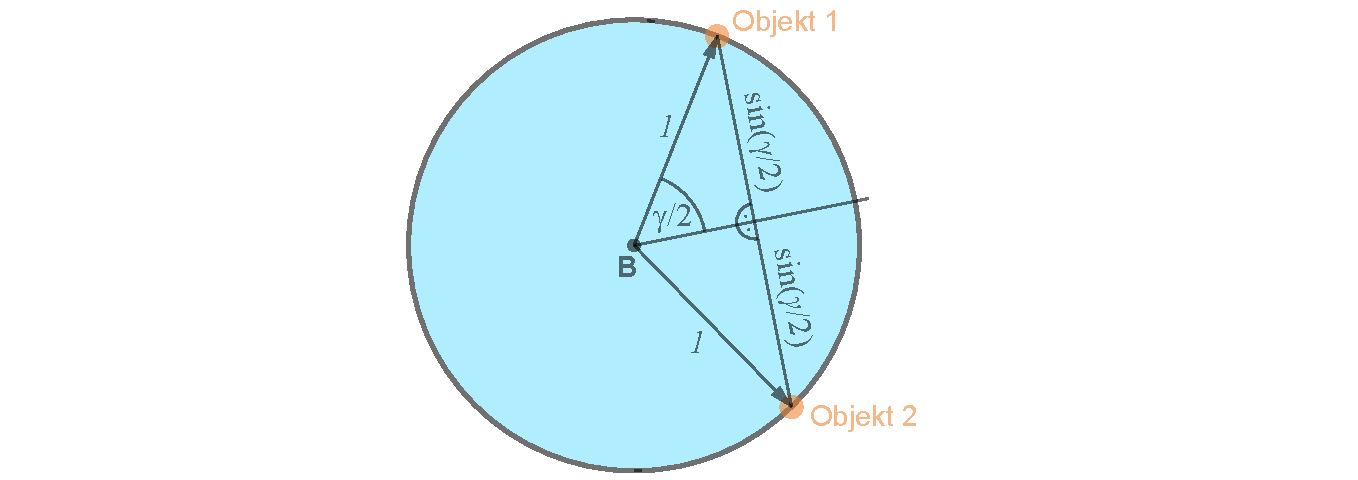
\includegraphics[width=0.75\columnwidth]{Winkelabstand.pdf}
\captionof{figure}{Winkelabstand zweier Himmelsk�rper.}\label{abb:hm_winkelabstand}
\end{center}
Man verwendet dann eine andere Formel.
Mit der L�nge des Differenzvektors $ d=\left|\vec{r}_1- \vec{r}_2\right| = \sqrt{(x_1-x_2)^2+(y_1-y_2)^2+(z_1-z_2)^2}$ ergibt sich dann 
$\gamma =\arcsin \lk \frac{d}{2} \rk $.\\
Bei Winkeln nahe $180\degree$ hat man immer noch ein Problem, da dort der Sinus des halben Winkels nahezu konstant ist.
Das l�st man dadurch, dass man den Winkelabstand $\bar{\gamma}$ von einem Objekt zum Antipoden des anderen berechnet.
Dieser Wert ist ja exakt um $180\degree$ verschoben, sodass $\bar{\gamma}$ wieder nahe bei $0\degree$ liegt.\\
	\item \emph{Es soll die k�rzeste Flugstrecke von St.~Petersburg (P) nach San Francisco (F) nahe der Erdoberfl�che berechnet werden (\figref{hm_Flug_SFO}, Geographische Breiten $\varphi_{\text{P}}=59.9\degree$, $\varphi_{\text{F}}=37.8\degree$ und geographische L�ngen $\lambda_{\text{P}}=30.3\degree$, $\lambda_{\text{F}}=-122.4\degree$), ebenso wie Anfangs- und Endkurs des Flugzeugs.}\\ 	\medskip 
Wir berechnen wieder den Winkelabstand zwischen den Punkten P und F.
Die k�rzeste Strecke ist dann -- wenn die Abplattung der Erde und die Flugh�he vernachl�ssigt werden -- der Abschnitt des Gro�kreises, der durch den Winkelabstand $\gamma$ definiert wird (siehe Abbildung):
$\overline{\text{PF}}=R_{\earth} \,,\gamma$, wobei $\gamma$ sich wie eben dargestellt berechnet.
Setzt man die Werte ein, erh�lt man $\overline{\text{PF}} \approx \SI{8867}{\kilo\metre}$.
Alternativ kann man die Berechnung nat�rlich �ber den Seiten-Kosinussatz der sph�rischen Trigonometrie machen.

\begin{center}

\includegraphics[width=\columnwidth]{Flug_SFO.pdf} \\ 
\captionof{figure}[Berechnung der k�rzesten Flugbahn zwischen zwei Orten.]{Berechnung der k�rzesten Flugbahn zwischen zwei Orten entlang der Erdoberfl�che.}\label{abb:hm_Flug_SFO} 
\end{center}

Die Anfangs- und Endkurse k�nnen wir mit dem Sinussatz aus dem Kugeldreieck $\Delta \text{F-NP-P}$ bestimmen, wobei wir die relative Richtung zu $N\!=\!360 \degree$ berechnen wollen:
\begin{align*}
	\sin\beta &=  \frac{\sin \lk \lambda_{\text{F}}-\lambda_{\text{P}} \rk}{\sin \gamma} \, \sin \lk 90 \degree - \varphi_{\text{F}} \rk ~~
	\Rightarrow \text{Kurs}_A = 360\degree - \beta \approx 338\degree ~~ \text{Anfangskurs und} \\
	\sin\alpha &=  \frac{\sin \lk \lambda_{\text{F}}-\lambda_{\text{P}} \rk}{\sin \gamma} \, \sin \lk 90 \degree - \varphi_{\text{P}} \rk ~~
	\Rightarrow \text{Kurs}_E = 180\degree + \alpha \approx 194\degree ~\text{Endkurs}.
\end{align*}
\end{enumerate} \label{bsp:laengengrad_abst_fl} 

\end{example}
%BEISPIEL %%%%%%%%%%%%%%%%%%%%%%%%%%%%%%%%%%%%%%%%%%%%%%%%%%%%%%%%%%%%%%%%%%%%%%%%%%%%%%%%%%

Mit der Sternzeit kommen wir direkt zur (wahren) \emph{Sonnenzeit}\index{Sonnenzeit!wahre} und k�nnen damit tats�chlich die b�rgerliche Zeit definieren \bzw genau messen.
Die Sonnenzeit ist wie die Sternzeit eine lokale Zeit.
Die Sternzeit ist 0 Uhr, wenn der Fr�hlingspunkt im Meridian steht.
Analog ist die Sonnenzeit 12 Uhr (mittags), wenn die Sonne den Ortsmeridian durchl�uft.
Man kann auch sagen, dass die Ortszeit der um 12 Stunden ($180\degree$) erh�hte Stundenwinkel der Sonne ist.
Die so definierte mittlere Ortszeit von Greenwich wird jetzt UT genannt und ist der um 12 Stunden erh�hte Stundenwinkel der fiktiven mittleren Sonne\index{Sonnenzeit!mittlere} in Greenwich\footnote{Die Addition von 12 Stunden ist n�tig, weil der Meridiandurchgang der fiktiven mittleren Sonne um 12:00 UT stattfinden soll, ihr Stundenwinkel in diesem Augenblick aber 0 betr�gt.}, \dh
\begin{equation}
\UT = 12\:\text{h} + \tau_\text{0, m. Sonne} \,.
\label{eq:hm_UT}
\end{equation} 
F�r Orte auf einem L�ngengrad $\lambda$ (in $\degree$) gilt analog zu \eqref{eq:hm_LMST}
\begin{equation}
\MOZ = \UT+ \frac{\lambda}{15} \lk \frac{\text{h}}{\degree} \rk \,.
\label{eq:hm_MOZ}\
\end{equation}
Die so definierte Sonnenzeit ergibt einen Sonnentag, der als Basis unserer Alltagszeit UT etwas l�nger ist als der oben definierte Sterntag. Die eigene Bewegung der Erde um die Sonne f�hrt dazu, dass die Zeit, bis die Sonne wieder kulminiert, etwas l�nger ist als die Zeit zwischen zwei Fixstern-Meridian-Durchg�ngen.
Nach einfacher Rechnung (Beispiel~\ref{bsp:sonnentag_sternentag}) findet man, dass der Sterntag gemessen an den 86400 (SI)-Sekunden des Sonnentags nur 23 Stunden, 56 Minuten und 4.0905 (SI)-Sekunden = 86125 (SI)-Sekunden lang ist.\footnote{Der Sterntag wird wieder in 24 Stunden unterteilt, die wir aber aus nachvollziehbaren Gr�nden und Respekt vor der Weltliteratur Stefan Zweigs hier nicht Sternstunden nennen.} % auskommentiert: hier gibt es keine Analogie. Genauso wenig bezeichnet ein Sonnentag einen Tag, an dem die Sonne scheint.}
Die Lage der fiktiven mittleren Sonne auf dem Himmels�quator kann nat�rlich nicht durch Beobachtung, sondern nur durch Rechnung bestimmt werden.
Nach \eqref{eq:hm_std_winkel_tau} gilt f�r den Meridiandurchgang der mittleren Sonne
\begin{equation}
\UT = 12\:\text{h} + \tau_\text{0, m. Sonne} = 12\:\text{h} + \theta_0 - \alpha_\text{0, m. Sonne} \,.
\label{eq:hm_UT_2}
\end{equation}

%BEISPIEL 2 %%%%%%%%%%%%%%%%%%%%%%%%%%%%%%%%%%%%%%%%%%%%%%%%%%%%%%%%%%%%%%%%%%%%%%%%%%%%%%%%%%
\begin{example}{Sonnentag und Sterntag}
  Wir wollen das Verh�ltnis von Sonnentag und Sterntag berechnen.
  Aus \figref{hm_Sterntag_Sonnentag} erkennt man, dass $\alpha\!=\!360\degree / n_\text{\astrosun}$, wobei $n_\text{\astrosun}$ die Zahl der Sonnentage pro tropischem Jahr bezeichnet. Das Verh�ltnis der Tagesl�ngen von Sonnentag $\text{d}_\text{\astrosun}$ zu Sterntag $\text{d}_\diamond$ ist dann:
\begin{equation*}
\frac{\text{d}_\text{\astrosun}}{\text{d}_\diamond} = \frac{360\degree + \frac{360\degree}{n_\text{\astrosun}}}{360\degree} = 1+\frac{1}{n_\text{\astrosun}} = 1+\frac{\text{d}_\text{\astrosun}}{\tau_\text{trop}} = \lk 1-\frac{\text{d}_\diamond}{\tau_{\text{trop}}} \rk^{-1}\,.
\end{equation*}
\begin{center}
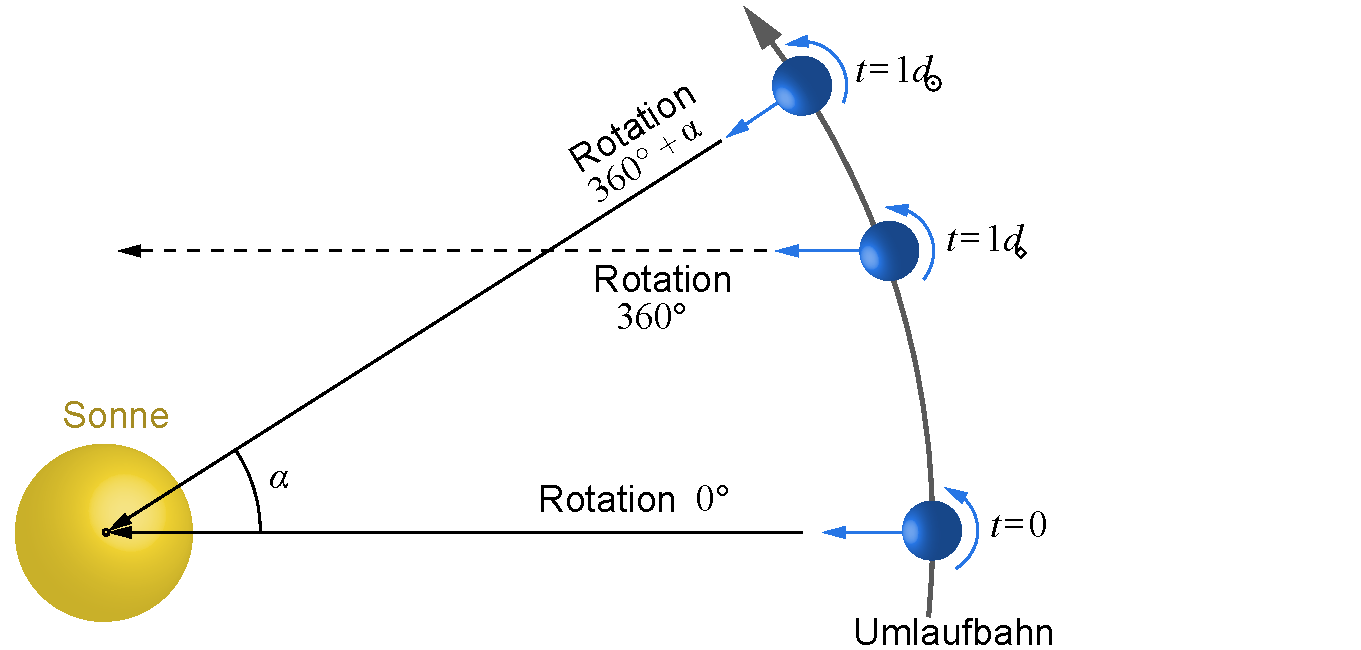
\includegraphics[width=0.8\columnwidth]{Sterntag_Sonnentag.pdf}% 
\captionof{figure}{Zum Unterschied zwischen Sterntag und Sonnentag.}\label{abb:hm_Sterntag_Sonnentag}
\end{center}
Mit $n_{\text{\astrosun}}\!=\! \frac{\tau_\text{trop}}{\text{d}_{\text{\astrosun}}} \! = \!365.242199 $ folgt daraus ${\text{d}_\text{\astrosun}}/{\text{d}_\diamond}\!=\!1.0027379$.
Der Sterntag ist damit um rund $1/365$ k�rzer als ein mittlerer Sonnentag und betr�gt $23$ Stunden $56$ Minuten und $4.0905$ Sekunden. \\

\label{bsp:sonnentag_sternentag}
\end{example}
%BEISPIEL %%%%%%%%%%%%%%%%%%%%%%%%%%%%%%%%%%%%%%%%%%%%%%%%%%%%%%%%%%%%%%%%%%%%%%%%%%%%%%%%%%

Auf Basis von \eqref{eq:hm_UT_2} wurde der Zusammenhang zwischen Weltzeit\index{Weltzeit} UT und der Greenwich Sternzeit\index{Greenwich Sternzeit} $\theta_0\!=\!\GMST(\UT)$ (\textit{Greenwich Mean Sideral Time})\index{Greenwich Mean Sideral Time} wie folgt festgelegt:
\begin{align} \label{eq:hm_UT_3}
\theta_0(\UT) =&\, 24110.5481\:\text{s}+8640184.812866\:\text{s}\, T_0+0.093104\:\text{s}\, T^2  \\
							 &+\mathcal{O}(T^3) + 1.0027379093\, \UT \nonumber \,,\\
\text{mit } T_0 = &\frac{\text{JD}_0-2451545.0}{36525}~~\text{und}~~T=\frac{\text{JD}-2451545.0}{36525}\,. \nonumber
\end{align}
Dabei sind $T_0$ und $T$ durch das jeweilige Julianische Datum um 0:00 des Beobachtungsdatums ($\text{JD}_0$) bzw. zur Uhrzeit des Beobachtungszeitpunkts (JD) gegeben.
Der lineare Term in \eqref{eq:hm_UT_3} gibt die Geschwindigkeit der fiktiven mittleren Sonne bez�glich des mittleren Fr�hlingspunkts an.
Das entspricht also multipliziert mit der Zeit einer Rektaszension.
Der quadratische Term ber�cksichtigt die weiter oben bereits erw�hnte pr�zessionsbedingte Bewegung des Fr�hlingspunkts.
Der Faktor $1.0027379093$ ergibt sich aus dem Unterschied zwischen Sonnentag  und Sterntag (Beispiel \ref{bsp:sonnentag_sternentag}).\footnote{Die L�nge des Sonnentages wird auch synodische Tagesl�nge\index{Periode!synodische}, die des Sterntages siderische Tagesl�nge\index{Periode!siderische} genannt.}
Gleichung \eqref{eq:hm_UT_3} stellt also einen Zusammenhang zwischen der Sternzeit und der Weltzeit UT her.
Obwohl die Weltzeit UT ihrer Definition gem�� eigentlich vom Sonnenlauf abzuleiten w�re, wird sie jedoch �ber \eqref{eq:hm_UT_3} aus den beobachteten Meridiandurchg�ngen von Sternen, also der Sternzeit, abgeleitet.
Das ist sinnvoll, da sich Sterndurchg�nge wesentlich pr�ziser beobachten lassen als die Position der �beraus hellen Sonne.
Man kann die Formeln aber nat�rlich auch benutzen, um die Sternzeit aus UT zu berechnen.

Nach diesen beiden mit einigen Definitionen versehenen Kapiteln haben wir nun die geeigneten Werkzeuge (Koordinatensysteme und Zeitdefinitionen), um die Mechanik der Himmelsk�rper beschreiben und vor allem auch Beobachtungsdaten ableiten \bzw berechnen zu k�nnen.
In der Himmelsmechanik wird im Grunde nichts anderes gemacht, als das Anfangswertproblem der entsprechenden Bewegungsgleichung f�r den oder die jeweiligen Himmelsk�rper  (Planeten, Monde, Kometen \ua) zu l�sen.
Die Bewegungsgleichung wollen wir nun als n�chstes aus den Gravitationsgesetzen herleiten. 
Wir werden dabei zun�chst allgemein, \dh ohne die Verwendung eines spezifischen Koordinatensystems, vorgehen.
Erst wenn wir Beobachtungsdaten und Ereignisse konkret berechnen, benutzen wir das jeweils passende r�umliche KOS.




\section{Bewegungsgleichung der Himmelsmechanik}\label{kap:hm_bewegungsgl}

In diesem Kapitel kommen wir zur grundlegenden Bewegungsgleichung der Himmelsmechanik.
In der Theorie der Gravitation ist die einfachste Konstellation eine aus zwei K�rpern, das sogenannte \emph{\gls{zkp}}\index{Zweik�rperproblem|textbf} (ZKP) (siehe Kapitel Physik der Bewegung im Band I). 
%Eine Bewegungsgleichung f�r das Zweik�rperproblem ist dabei eine Gleichung zur Bestimmung der Koordinaten der beiden K�rper im Raum als Funktion der Zeit.
Die entsprechende Bewegungsgleichung der Himmelsmechanik hei�t \emph{Kepler-Gleichung}.\index{Kepler-Gleichung|textbf}\indexp{Kepler, Johannes}\footnote{Johannes Kepler (1571 -- 1630 ) war ein deutscher Astronom und Physiker. Er entdeckte die Gesetzm��igkeiten, nach denen sich Planeten um die Sonne bewegen, die nach ihm benannten Keplerschen Gesetze, womit er zu den Begr�ndern der modernen Naturwissenschaften geh�rt. Wir schreiben wie sonst im Buch auch entsprechend der verwendeten Notation \emph{Kepler-Gleichung}, analog Lagrange-Gleichung, Euler-Gleichung usw. In der Astronomie hat sich historisch \emph{Keplergleichung} als  Konvention herausgebildet.} 
Die Bewegungsgleichung der Himmelsmechanik hei�t \emph{Kepler-Gleichung}.\index{Kepler-Gleichung|textbf}\indexp{Kepler, Johannes}\footnote{Johannes Kepler (1571 -- 1630 ) war ein deutscher Astronom und Physiker. Er entdeckte die Gesetzm��igkeiten, nach denen sich Planeten um die Sonne bewegen, die nach ihm benannten Keplerschen Gesetze, womit er zu den Begr�ndern der modernen Naturwissenschaften geh�rt. Wir schreiben wie sonst im Buch auch entsprechend der verwendeten Notation \emph{Kepler-Gleichung} (analog Lagrange-Gleichung, Euler-Gleichung usw.). In der Astronomie hat sich aber historisch \emph{Keplergleichung} als  Konvention herausgebildet.} 
Obwohl sie f�r die Himmelsmechanik eine fundamentale Bedeutung hat, wird die Kepler-Gleichung im Physik-Studium kaum behandelt.
Wir wollen sie deshalb hier zun�chst aus der Newtonschen Gravitationstheorie herleiten und auch eine auf Johannes Kepler selbst zur�ckgehende einfache geometrische Herleitung angeben.
Im Anschluss zeigen wir, wie man L�sungen f�r die Kepler-Gleichung erhalten kann und wie diese \zb f�r das Sonne-Erde- oder Sonne-Planeten-Problem aussehen.
Wir werden sp�ter auch sehen, dass dieser einfachen L�sungsansatz bereits f�r das Mond-Erde-System wegen der Einfl�sse der Sonne und der anderen Planeten  nicht mehr ausreicht.

\subsection{Herleitung der Kepler-Gleichung} \label{kap:hm_abl_kepler}
Die physikalischen Grundlagen der Bewegung des ZKP hatten wir uns bereits im Kapitel Physik der Bewegung im Band I angeeignet.
In \kap{hm_zeitdefinition} benutzten wir bei der Definition einiger KOS das Ergebnis, dass die Bewegung von Himmelsk�rpern in Bahnebenen stattfindet. Wir zeigen als Wiederholung noch einmal (diesmal in astronomischer Notation), dass sich die Bewegung in einer Ebene direkt aus der Tatsache ergibt, dass die Newtonsche Gravitationskraft eine Zentralkraft ist. 
Wir betrachten dazu das ZKP nach \figref{hm_2kp}, wobei wir den K�rper mit der Masse $M$ als wesentlich schwerer annehmen und deshalb als Zentralk�rper bezeichnen.
Den K�rper mit der wesentlich kleineren Masse $m$ wollen wir hingegen einfach Planet P nennen, obwohl es auch ein beliebiger anderer Himmelsk�rper (\zb Komet) sein kann.
Mit $\vec{r}_\text{M}$ und $\vec{r}_\text{m}$ bezeichnen wir die Vektoren vom Ursprung O eines beliebigen KOS zu den Massen $M$ \bzw $m$.
Der Vektor $\vec{r}=\vec{r}_\text{m}-\vec{r}_\text{M}$ zeigt vom Zentralk�rper zum Planeten.

\begin{figure}
\begin{minipage}{\textwidth}
\leftfigure{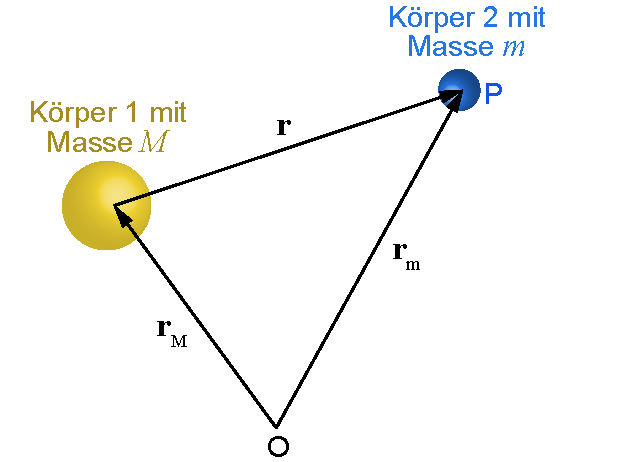
\includegraphics[width=0.5\textwidth]{ZKP.pdf}}
\hspace{\fill}
\rightfigure{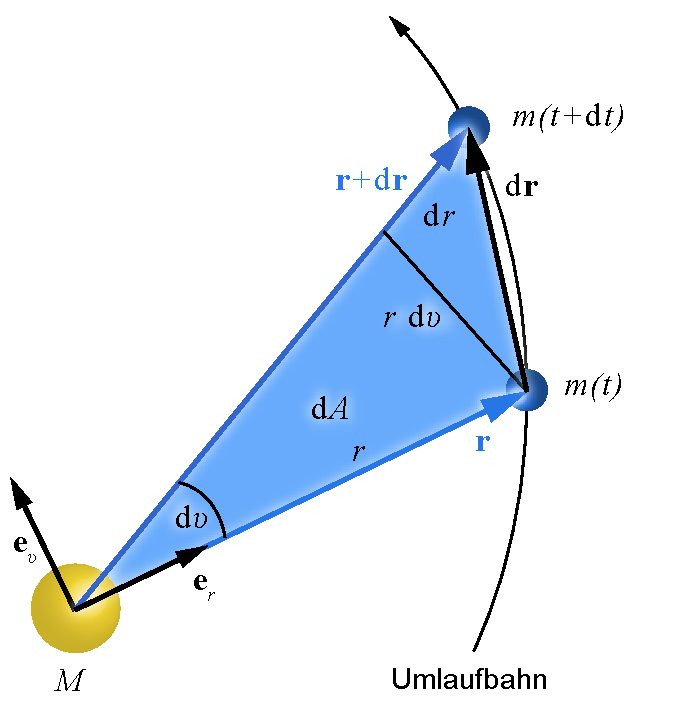
\includegraphics[width=0.5\textwidth]{Flaechensatz.pdf}}
\leftcaption{Zur Herleitung des Zweik�rperproblems.}\label{abb:hm_2kp}
\rightcaption{Fl�chensatz.} \label{abb:hm_flaechensatz}
\end{minipage}
\end{figure}

Laut Newtons Gravitationsgesetz\index{Gravitation} wirkt auf den K�rper mit der Masse $m$ (Planet) durch den Zentralk�rper mit der Masse $M$ (\zb die Sonne) eine Kraft
\begin{equation}
\vec{F}_\text{m} = m\,\ddot{\vec{r}}_\text{m} = -\frac{G \, M \, m}{r^3} \, \vec{r} \,.
\label{eq:hm_beschl_zk}
\end{equation}
Entsprechend wirkt auf den Zentralk�rper durch den Planeten die Kraft
\begin{equation}
\vec{F}_\text{M} = M\,\ddot{\vec{r}}_\text{M} = +\frac{G \, m \, M}{r^3} \, \vec{r} \,.
\label{eq:hm_beschl_pl}
\end{equation}
Die Beschleunigungen erh�lt man durch Division durch die Massen $m$ bzw. $M$:
\begin{equation}
\ddot{\vec{r}}_\text{m}-\ddot{\vec{r}}_\text{M} = \ddot{\vec{r}} = -\frac{G(M+m)}{r^3}\, \vec{r} = -\frac{\mu_\text{G}}{r^3}\, \vec{r}
\label{eq:hm_zk-pl}
\end{equation}
mit 
\begin{equation}
\mu_\text{G}\!=\!G\,(M+m). 
\label{eq:hm_def_muG}
\end{equation}
Hierin ist $G\!=\!\SI{6.673e-11}{\metre\cubed\per\kg\per\second\squared}$ die bereits in Band I eingef�hrte \emph{Gravitationskonstante}\glslink{gravkonst}.\index{Gravitationskonstante}\footnote{Man kann die Relativkoordinate auch so w�hlen, dass der Ort des Massenschwerpunkts $\vec{r}_\text{S}$ des Systems den Ursprung O des KOS bildet. Dann ist $\vec{r}_\text{S} = (M \vec{r}_\text{M} + m \vec{r}_\text{m})/(M+m)=0$ und die Bewegungsgleichung f�r den Planeten lautet $\ddot{\vec{r}} = -\mu_\text{G} \vec{r}/r^3 $ mit $\mu_\text{G}\!=\!GM (1 + m/M)^{-2}$, was f�r $ m \ll M$ in \eqref{eq:hm_def_muG} �bergeht.} %und $\mu_\text{G}$ der sogenannte \gls{gravparhm}.  
Zur eindeutigen L�sung von $\vec{r}(t)$ in \eqref{eq:hm_zk-pl} werden f�r das Differentialgleichungssystem 2.
Ordnung (in der Zeit) mit drei r�umliche Koordinaten folglich sechs Konstanten (Bewegungsintegrale \bzw Anfangsbedingungen) ben�tigt.
Wir wollen diese im Folgenden einzeln bestimmen. 

\subparagraph{\textbf{Drehimpulsintegral:}}\index{Drehimpulsintegral}
Wir beginnen mit der Herleitung des Drehimpulsintegrals\index{Drehimpulsintegral} und bilden dazu das Kreuzprodukt von $\vec{r}$ mit \eqref{eq:hm_zk-pl}:
\begin{equation*}
\vec{r} \times \ddot{\vec{r}} = -\frac{\mu_\text{G}}{r^3}\,  \vec{r} \times \vec{r} = 0 \,.\\
\end{equation*}
Es gilt aber auch
\begin{equation*}
\frac{\D }{\D t} \lk \vec{r} \times \dot{\vec{r}}\rk = \underbrace{\dot{\vec{r}} \times \dot{\vec{r}}}_{=0} + \underbrace{\vec{r} \times \ddot{\vec{r}}}_{=0} = 0 \; ,
\end{equation*}
woraus nach Integration sofort 
\begin{equation}
\vec{r} \times \dot{\vec{r}} = \vec{L} = \vec{const} 
\label{eq:hm_kepler1}
\end{equation}
folgt.
Der in \eqref{eq:hm_kepler1} definierte konstante Vektor $\vec{L}$ ist (bis auf den Faktor $m$ bzw. $m_\text{eff}$) gleich dem \gls{drehimpuls} des Planeten in Bezug auf den Zentralk�rper.
Er wird daher auch als \emph{spezifischer} Drehimpuls bezeichnet und ist also eine Konstante.
Gleichung \eqref{eq:hm_kepler1} wird daher als Drehimpulsintegral bezeichnet.
Wir werden ab jetzt wie in der Himmelsmechanik und Astronomie �blich die spezifischen Gr��en\footnote{H�ufig benutzt man auch f�r die spezifischen Gr��en Kleinbuchstaben oder griechische Symbole, also \zb f�r den Drehimpuls $\vec{l}$ \bzw $\vec{\lambda}$ anstelle $\vec{L}$. Wir bleiben aber im Folgenden bei den Gro�buchstaben, die auch den historisch in der Astronomie eingef�hrten Bezeichnungen und Symbolen entsprechen.} verwenden, man spart sich damit etwas Schreibarbeit und die Gleichungen werden �bersichtlicher.
Das ist im �brigen ein in der Physik �bliches Vorgehen, bei dem aber immer etwas Aufmerksamkeit angesagt ist.
Wir haben deshalb den Zusammenhang zwischen
den \anf{physikalischen} Gr��en aus Kapitel 1 (Band I)
und den hier verwendeten astronomischen Gr��en in Tabelle \ref{tab:hm_notation_hm} gelistet.%
\footnote{Es sei noch erw�hnt, dass \eqref{eq:hm_kepler1}
nur dann den spezifischen Drehimpuls des Planeten darstellt,
wenn dessen Masse sehr viel kleiner als die Masse
des Zentralk�rpers ist.
Im Fall $M\!\approx\!m$ gibt $\vec{L}$ nicht mehr
den Drehimpuls eines einzelnen K�rpers an.}
Da $\vec{L}$ senkrecht zu $\vec{r}$ und $\dot{\vec{r}}$
und konstant ist, findet die Bewegung in einer Ebene statt.
Dies ist eine der Aussagen des \emph{1.~Keplerschen Gesetzes}.
Aus der Konstanz des Drehimpulses $\vec{L}$ folgt sofort auch das \emph{2.~Keplersche Gesetz} (Fl�chensatz), da $\abs{\vec{r}\times\dot{\vec{r}}\,\D t}\!=\!\abs{\vec{r}\times\D \vec{r}}$ der doppelten Fl�che des von den Vektoren $\vec{r}$ und $\D \vec{r}$ aufgespannten Dreiecks entspricht.
Das ist aber gleich der Fl�che $\D A$, die von $\vec{r}$ in der Zeit $\D t$ �berstrichen wird (siehe \figref{hm_flaechensatz}). 

Wegen der Bewegung in einer Ebene sind f�r die Behandlung vieler Probleme Polarkoordinaten vorteilhaft.
Wir geben deshalb vielfach neben der vektoriellen Darstellung auch die Formulierung in Polarkoordinaten an.
Aus \figref{hm_flaechensatz} k�nnen wir direkt die ersten Ableitungen der (zeitabh�ngigen) Einheitsvektoren $\vec{e}_r$ und $\vec{e}_{\upsilon}$ ablesen (Drehung um den Ursprung mit Winkel $\D \upsilon$.):
\begin{equation*}
\dot{\vec{e}}_r \! = \dot{\upsilon} \, \vec{e}_{\upsilon}  ~\;\text{und} \;\dot{ \vec{e}}_{\upsilon} = -\dot{\upsilon} \, \vec{e}_{r} \,.
\end{equation*}
Hieraus bestimmt sich aus $\vec{r}\!=\!r\, \vec{e}_r$ und $\D \vec{r}\! = \!\D r \, \vec{e}_r + r\,\D  \upsilon \, \vec{e}_{\upsilon} $ die Geschwindigkeit $ \dot{\vec{r}}$ sofort zu 
\begin{align}
\dot{\vec{r}}\! = \!\vec{v}\!=\!\dot{r}\, \vec{e}_r + r\dot{\upsilon}\,\vec{e}_{\upsilon} ~. \label{eq:hm_vectoren_polar}
\end {align}
Nochmalige Anwendung der Differentiation auf $\dot{\vec{r}}$ f�hrt zu
\begin{equation}
\ddot{\vec{r}}\! =\!(\ddot{r}-r\dot{\upsilon}^2)\,\vec{e}_r + (2 \dot{r}\dot{\upsilon}+r\ddot{\upsilon})\,\vec{e}_{\upsilon} . \label{eq:hm_beschl_polar}
\end{equation}
Damit k�nnen wir den Drehimpuls und seinen Betrag schreiben:
\begin{equation}
\vec{L} = \vec{r}\times\dot{\vec{r}} = r^2 \dot{{\upsilon}} \veceZ \; , \label{eq:hm_drehimp_z}
\end{equation}
\begin{equation}
L=r^2\dot{\upsilon} ~. \label{eq:hm_drehimp_z_polar}
\end{equation}

\subparagraph{\textbf{Energieintegral:}}\index{Energieintegral}
Als N�chstes wollen wir ein Ma� f�r die \glslink{energie}{Gesamtenergie}\index{Energieintegral} des ZKP bestimmen.
Da das System konservativ ist, muss diese ja eine Erhaltungsgr��e sein.
Dazu bilden wir das Skalarprodukt von $\vec{v}\!=\!\dot{\vec{r}}$ mit $\ddot{\vec{r}}$:
\begin{align}
\begin{split}
\vec{v} \cdot \dot{\vec{v}} &= \vec{v} \cdot \ddot{\vec{r}} = -\frac{\mu_\text{G}}{r^3}\,\vec{v} \cdot \vec{r} = -\frac{\mu_\text{G}}{r^3}\,\dot{\vec{r}} \cdot \vec{r}  \\
 &= -\mu_\text{G} \frac{\dot{r}r}{r^3} = -\mu_\text{G} \frac{\dot{r}}{r^2} = \mu_\text{G}\,\frac{\D }{\D t} \lk \frac{1}{r}\rk \,.
\end{split} \label{eq:hm_v_mal_vpunkt_1}
\end{align}
Andererseits gilt
\begin{equation}
\vec{v} \cdot \dot{\vec{v}} = \frac{\D }{\D t} \lk \frac{v^2}{2} \rk \label{eq:hm_v_mal_vpunkt_2} .\\
\end{equation}
Daraus folgt mit {\eqref{eq:hm_v_mal_vpunkt_1}
\begin{equation}
\frac{\D }{\D t} \lk \frac{v^2}{2} - \frac{\mu_\text{G}}{r}\rk = 0 \label{eq:hm_v_mal_vpunkt_3}
\end{equation}
und nach Integration
\begin{equation}
\frac{v^2}{2} - \frac{\mu_\text{G}}{r} = H = \con\:. \label{eq:hm_bewgl1}
\end{equation}
Auf der linken Seite von \eqref{eq:hm_bewgl1} steht die durch $m$ dividierte Summe aus kinetischer und \glslink{potential-hm}{potentieller Energie} des umlaufenden K�rpers.
Diese Summe $H$ ist wie erwartet f�r ein konservatives System\index{System!konservatives} konstant.\footnote{Wir verwenden den Buchstaben $H$ f�r die Energie, da die ansonsten �bliche Bezeichnung $E$ aus historischen Gr�nden f�r die weiter unten eingef�hrte exzentrische Anomalie reserviert ist.}
Man erkennt aus dem Energieintegral ferner, dass f�r $H\!<\!0$ die Bewegung r�umlich beschr�nkt sein muss.
Damit $\mu_\text{G}/r\!>\!v^2/2$ bleibt, kann $r$ nicht unendlich werden.

\subparagraph{\textbf{Laplace-Integral (Richtungsintegral):}}\index{Laplace-Integral}\index{Richtungsintegral}\indexp{Laplace, Pierre-Simon (Marquis) de}

Wir bilden nun noch das Vektorprodukt aus $\vec{L}$ und $\ddot{\vec{r}}$:
\begin{equation*}
\vec{L} \times \ddot{\vec{r}} = \lk \vec{r} \times \dot{\vec{r}}\rk \times \lk \frac{-\mu_\text{G}}{r^3} \rk\, \vec{r} \,.
\end{equation*}
Man findet nach etwas Vektoralgebra (\probref{hm_laplace}) eine weitere Integrationskonstante, die wir als \emph{Laplace-Vektor}\index{Laplace-Vektor} $\vec{e}$ der Bewegung bezeichnen:
\begin{equation}
\vec{L} \times \dot{\vec{r}} + \lk \frac{\mu_\text{G}}{r} \rk \, \vec{r} = \vec{const} = -\mu_\text{G} \, \vec{e} \,. \label{eq:hm_laplace_int}
\end{equation}
Dieser Vektor, der in der (vor allem angels�chsischen) Literatur oft auch als Runge\footnote{Carl David Tolm� Runge (1856--1927) war ein deutscher Mathematiker, der auf zahlreichen Gebieten der Mathematik und mathematischen Physik forschte. In Band I hatten wir Runge bereits im Zusammenhang mit dem Runge-Kutta-Verfahren kennen gelernt.}-Lenz\footnote{Wilhelm Lenz (1888--1957) war ein deutscher Physiker, der an der Universit�t Hamburg lehrte und auf zahlreichen Gebieten der Physik aktiv war. Er f�hrte \ua den Runge-Lenz-Vektor in die Quantenmechanik ein.}-Vektor\index{Runge-Lenz-Vektor} bezeichnet wird, liegt in der Bahnebene und gibt eine Vorzugsrichtung innerhalb der Bahnebene vor.
Der Laplace-Vektor ist aber nicht v�llig unabh�ngig von den beiden anderen Bewegungsintegralen.
Man kann unter Benutzung von \eqref{eq:hm_kepler1} und \eqref{eq:hm_bewgl1} zeigen, dass $\vec{L}\cdot \vec{e}\!=\!0$ und dass demzufolge die Beziehungen
\begin{equation}
\mu_\text{G}^2 \, \lk \abs{\vec{e}}^2 - 1 \rk = 2H \, \abs{\vec{L}}^2 ~~~\text{\bzw}~~~~ e^2 = \frac{2H L^2}{\mu_\text{G}^2} + 1  
\label{eq:hm_relations1}
\end{equation}
gelten (\probref{hm_laplace}).
Der Betrag $\abs{\vec{e}}\!=\!e$ des Laplace-Vektors wird \emph{(numerische) Exzentrizit�t}\footnote{In der Mathematik wird die numerische Exzentrizit�t im Allgemeinen mit $\epsilon$ bezeichnet, w�hrend dort $e=\sqrt{a^2-b^2}$ f�r die lineare Exzentrizit�t steht.
Da $\epsilon$ in der Himmelsmechanik f�r die Neigung der Erdachse reserviert ist, bleiben wir bei der Nutzung von $e$ f�r die (numerische) Exzentrizit�t (siehe auch Tabelle \ref{tab:hm_notation_hm} im Tabellenanhang.)} genannt und ist nach \eqref{eq:hm_relations1} durch die Energie und den Drehimpuls vollst�ndig festgelegt.
\vec{e} liefert dann nur noch als unabh�ngige Gr��e einen Winkel bzw. eine Richtung.
Wir haben nun f�nf unabh�ngige Konstanten $\vec{L}$ (3 Komponenten), $H$ und die Richtung von $\vec{e}$ innerhalb der Bahnebene aus den Bewegungsintegralen gewonnen, die wir als physikalische Bahnparameter betrachten k�nnen.
Als sechsten Parameter nutzen wir eine Anfangsbedingung, \zb die Bahnposition des K�rpers zu einem bestimmten Zeitpunkt.
Wir arbeiten wieder mit den Polarkoordinaten $r$ und $\upsilon$, wobei wir die beliebig w�hlbare Bezugsrichtung des Polar-KOS in Richtung von $\vec{e}$ legen wollen.
Den Winkel $\upsilon$ zu dieser Bezugsachse wollen wir ab jetzt, wie in der Astronomie �blich, als \emph{wahre Anomalie}\index{Anomalie!wahre|textbf}\footnote{Der Begriff \anf{Anomalie} (\emph{altgriechisch} f�r Unebenheit, Unregelm��igkeit) geht auf die antiken Astronomen zur�ck, die den Winkel in der Bahnbewegung als abweichend und unregelm��ig von der erwarteten \anf{harmonischen} Kreisbahn beobachteten.
Historisch hat sich f�r die wahre Anomalie die Bezeichnung mit dem griechischen Buchstaben Ypsilon $\upsilon$ (\figref{hm_polarkoord}) herausgebildet.} bezeichnen.\\

\begin{figure}
\begin{minipage}{\textwidth}
\leftfigure{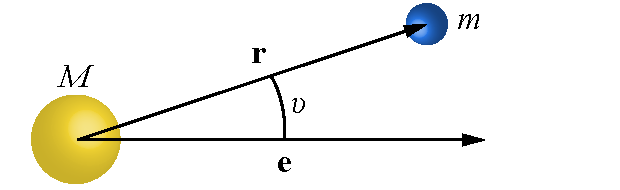
\includegraphics[width=0.5\textwidth]{Polarkoordinaten.pdf}}
\hspace{\fill}
\rightfigure{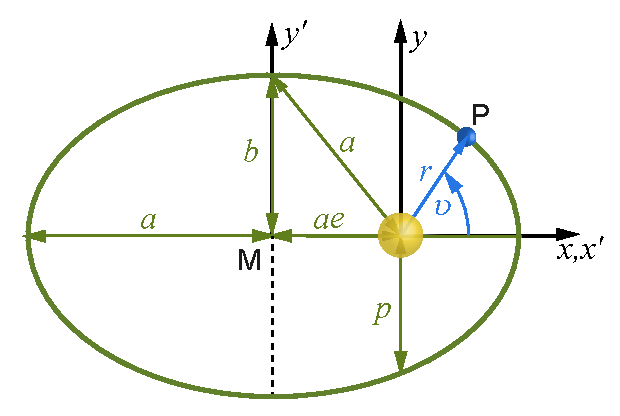
\includegraphics[width=0.5\textwidth]{Geometrie_der_Ellipse.pdf}}
\leftcaption{Polarkoordinaten.}\label{abb:hm_polarkoord}
\rightcaption[Geometrie der Ellipse.]{Geometrie der Ellipse. Man beachte die beiden Koordinatensysteme, das $x$-$y$-\KOS hat den Ursprung im Brennpunkt der Ellipse, das sogenannte Mittelpunkts-$x'$-$y'$-\KOS im Mittelpunkt.}\label{abb:hm_ellipse}
\end{minipage}
\end{figure}

Mit der Bezugsrichtung von $\vec{e}$ schreiben wir das Skalarprodukt $\vec{r} \cdot \vec{e}$ als
\begin{align}
\begin{split}
\vec{r} \cdot \vec{e} &= -\vec{r} \cdot \lk \frac{\vec{L}\times \dot{\vec{r}}}{\mu_\text{G}} + \frac{\vec{r}}{r} \rk \\
                      &= - \frac{\vec{r} \cdot ( \vec{L} \times \dot{\vec{r}} )}{\mu_\text{G}} - r = \frac{(\vec{r} \times \dot{\vec{r}}) \cdot \vec{L}}{\mu_\text{G}} - r = \frac{L^2}{\mu_\text{G}} - r = re\,\cos \upsilon \; ,
\end{split} \label{eq:hm_relations2}
\end{align}
woraus
\begin{align}
r(\upsilon) = \frac{L^2}{\mu_\text{G}}\,\frac{1}{1+e\,\cos \upsilon} = \frac{p}{1+e\,\cos \upsilon} \label{eq:hm_kegelschnitt}
\end{align}
folgt.
Wir haben damit f�r die Form der Bahn die Gleichung f�r Kegelschnitte\index{Kegelschnitt} erhalten.
Der sogenannte Halb-Parameter $p\!=\!L^2/\mu_\text{G}$ wird \emph{semi-latus rectum} genannt.
Dies ist der Abstand des Planeten zum Zentralk�rper bei einem Winkel $\upsilon = \pm\pi/2$ (\figref{hm_ellipse}).
Folgende Schlussfolgerungen kann man aus Gleichung \eqref{eq:hm_kegelschnitt} ziehen:
\begin{itemize}
	\item F�r $\cos\upsilon\!=\!1$ bzw. $\upsilon\!=\!0$, d.\,h. f�r die Richtung von $\vec{e}$, finden wir den Punkt der Bahn, der dem Zentralk�rper am n�chsten kommt.
          Dies ist die sogenannte \index{Periapsis}\emph{\gls{periapsis}} (im Fall der Sonne als Zentralk�rper das \index{Perihel|textbf}\emph{\gls{perihel}}).
          Damit wird der Begriff des Richtungsintegrals f�r den Laplace-Vektor verst�ndlich.
	\item F�r $\cos\upsilon\!=\!-1$ bzw. $\upsilon\!=\! \pi$, d.\,h. in entgegengesetzter Richtung von $\vec{e}$, erhalten wir den Punkt der Bahn, der dem Zentralk�rper am fernsten liegt.
          Dies ist die \index{Apoapsis}\emph{\gls{apoapsis}} (im Fall der Sonne als Zentralk�rper das \index{Aphel|textbf}\emph{\gls{aphel}}).
	\item F�r $\cos\upsilon\!=\!0$, also $\upsilon\!=\!\pm\pi/2$ ergibt sich $r\!=\!p$.
	\item F�r den Fall $0\!<\!e\!<\!1$ ergibt sich aus \eqref{eq:hm_relations2} als Bahn eine Ellipse.
          In diesem Fall ist auch nach \eqref{eq:hm_relations1} die Energie $H\!<\!0$. 
	\item F�r $e\!=\!1$ ergibt \eqref{eq:hm_kegelschnitt} eine Parabel und f�r $e\!>\!1$ eine Hyperbel.
          Wir sehen, dass die genaue Form der Bahn von den Parametern $L$ (Drehimpuls) und $e$ (Exzentrizit�t) und damit nach \eqref{eq:hm_relations1} auch von der Energie des Systems abh�ngt.
\end{itemize}
Wir wollen uns im Folgenden auf \emph{Ellipsenbahnen}\index{Ellipsenbahnen} (\figref{hm_ellipse}) beschr�nken.
F�r eine Ellipsenbahn wird die \glslink{groszehalbachse}{gro�e Halbachse} mit $a$ bezeichnet und die \glslink{kleinehalbachse}{kleine} mit $b$.
F�r $e$ gilt dann $0<e=\sqrt{1-\frac{b^2}{a^2}}<1$.
Damit ergeben sich f�r den kleinsten und den gr��ten Abstand des umlaufenden Planeten folgende Beziehungen:
\begin{align}
r_\text{min} &= \frac{L^2}{\mu_\text{G}} \frac{1}{1+e}~~\,, ~~r_\text{max} = \frac{L^2}{\mu_\text{G}} \frac{1}{1-e} \,. \label{eq:hm_aphel_perihel} 
\end{align}
Mit $r_\text{min}\!+\!r_\text{max}\!=\!2a$ folgt daraus
\begin{equation}
L = r^2\dot{\upsilon} = \sqrt{a\,\mu_\text{G}(1-e^2)} \,,  \label{eq:hm_drehimpuls_von_ae}
\end{equation}
womit wir einen Zusammenhang von physikalischen Bahnparametern ($L$) und geometrischen Parametern der Bahn ($a$, $e$) hergestellt haben.
Die Bahngleichung $r(\upsilon)$ schreiben wir dann mit den geometrischen Bahnparametern $a$ und $e$ in der �blichen Form:
\begin{equation}
r(\upsilon) = \frac{a(1-e^2)}{1+e\,\cos \upsilon} = \frac{p}{1+e\,\cos \upsilon}\,. \label{eq:hm_bahnglg}
\end{equation}
Wir leiten jetzt noch das \emph{3. Keplersche Gesetz} her, indem wir die Beziehung f�r den Drehimpuls \eqref{eq:hm_drehimpuls_von_ae} �ber die gesamte Ellipse, \dh �ber eine ganze Umlaufperiode $T_\text{P}$, integrieren:\footnote{Wir erinnern an die geometrische Interpretation des Drehimpulses als 2 $\D A /\D t$ im Rahmen der Herleitung des 2.\ Keplerschen Gesetzes.}
\begin{equation}
A = \frac{1}{2} \int\limits_0^{T_\text{P}} L\,\D t = \frac{1}{2}\, L\,T_\text{P} = \frac{1}{2}\sqrt{a \mu_\text{G}\lk 1-e^2\rk } \,T_\text{P} \,. \label{eq:hm_bahnglg_a}
\end{equation}
Andererseits ist der Fl�cheninhalt einer Ellipse $A\!=\!\pi a b\!=\! \pi a^2\sqrt{1-e^2}$.
Daraus folgt durch Quadrieren von \eqref{eq:hm_bahnglg_a} und Gleichsetzen mit \eqref{eq:hm_bahnglg}
\begin{equation}
\frac{T_\text{P}^2}{a^3} = \frac{4\pi^2}{\mu_\text{G}} = \con = \frac{4\pi^2}{GM} ~.
\label{eq:hm_3_kepler_gesetz}
\end{equation}
Die Quadrate der Umlaufperioden zweier Planeten um einen Zentralk�rper verhalten sich wie die Kuben ihrer gro�en Halbachsen. \\
Wir m�ssen hier eine Bemerkung zu der Umlaufzeit $T_\text{P}$ machen: Diese Zeit ist als siderische Umlaufzeit\glslink{siderischeumlaufzeit}\ definiert, \dh als die Zeit, die ein Planet f�r einen vollst�ndigen Umlauf braucht, um \zb die Sonne wieder vor dem gleichen Fixsternhintergrund zu sehen.
Diese Umlaufzeit l�sst sich aber nur f�r die Erde direkt bestimmen.
F�r alle anderen Planeten muss man sie aus der \glslink{synodischeumlaufzeit}{synodischen Umlaufzeit} berechnen.
Diese ergibt sich, wenn der andere Planet von der Erde aus betrachtet wieder im gleichen Winkelabstand zur Sonne steht.
Zum Gl�ck hatte Kepler sehr genaue Aufzeichnungen von Tycho Brahe\footnote{Tycho Brahe\indexp{Brahe, Tycho} (1546--1601) war ein bedeutender d�nischer Astronom. Seine Beobachtungen, die Kepler erst nach Brahes Tod auswertete, bildeten die Grundlage f�r die Ableitung der Keplerschen Gesetze (siehe auch \cite{Hecht2019}). Brahe f�hrt die Beobachtung vor gut 400 Jahren in der damals leistungsst�rksten Sternwarte der Welt auf der kleinen Insel Ven im �resund zwischen Kopenhagen und Malm� durch, wobei er mit exzellenten Winkelmessinstrumenten, aber ohne Teleskop arbeitete, das damals noch unbekannt war.}, die ihm die Berechnung der siderischen Umlaufzeit des Mars erm�glichten.
In \probref{hm_sideric_period_mars} kann die Berechnung Keplers f�r die Beobachtung von Mars-\glslink{opposition}{Oppositionen}\index{Mars-Opposition} nachvollzogen werden.
Bahnberechnungen f�r die Planeten unseres Sonnensystems sind im \mscr{} \mlhmref{InnerePlaneten.m} zu finden. 

\subparagraph{\textbf{vis-viva-Gleichung:}}
Wir wollen noch eine weitere wichtige Beziehung herleiten, und zwar die zwischen der Himmelsk�rperposition (Abstand zum Zentralk�rper) und seiner Bahngeschwindigkeit am jeweiligen Ort.
Diese Relation wird als \gls{visvivahm}\index{vis-viva-Gleichung}\footnote{Diese Formel wurde erstmalig von Gottfried Wilhelm Leibniz (1646--1716), einem der letzten gro�en Universalgelehrten, gefunden.} bezeichnet und ergibt sich, indem in \eqref{eq:hm_bewgl1} f�r $H$ die Gleichung \eqref{eq:hm_relations1} und f�r $L$ die Beziehung \eqref{eq:hm_drehimpuls_von_ae} eingesetzt wird. Wir erhalten die 
\begin{merksatz}  {vis-viva-Gleichung (\bzw den vis-viva-Satz)}
\begin{equation}
v^2 = \mu_\text{G} \lk \frac{2}{r} - \frac{1}{a} \rk \, \label{eq:hm_vis-viva}
\end{equation}\\

\end{merksatz}

und k�nnen damit zu jedem Punkt der Bahn (gegeben durch den Abstand $r$) die dort vorhandene Bahngeschwindigkeit $v$ bestimmen. 

In der Bahngleichung \eqref{eq:hm_bahnglg} stecken mit $a$ und $e$ nur zwei der sechs notwendigen Bahnparameter (Integrationskonstanten).
Das ist nicht verwunderlich, da wir uns ja mit den $r,\upsilon$-Koordinaten quasi in die Bahnebene \anf{gelegt} haben.
Zur vollen r�umlichen und zeitlichen Beschreibung der Bewegung muss diese Ebene noch im dreidimensionalen Raum positioniert und eine Anfangsbedingung festgelegt werden.
Dazu benutzt man, wie bereits in \kapitel{hm_koordinatensysteme} beschrieben, eine Bezugsebene und eine Bezugsrichtung, relativ zu denen die Bahnebene positioniert wird.
F�r unser Sonnensystem ist das sinnvollerweise das heliozentrisch-ekliptikale KOS, woraus sich drei weitere geometrische Bahnparameter, n�mlich $\omega$ (\glslink{argperiapsis}{Argument des \gls{perihel}s}), $\Omega$ (\glslink{laengeaufstknoten}{L�nge des \glslink{aufstknoten}{aufsteigenden Knotens}}\footnote{Alternativ zu $\Omega$ kann auch der Parameter $\varpi=\omega+\Omega$ verwendet werden. Bei dem aus historischen Gr�nden verwendeten Buchstaben $\varpi$ handelt es sich um eine Variante des griechischen $\pi$.}), und $i$ (Neigung der Bahn gegen die Ekliptik) ergeben (\figref{hm_bahnelemente}).
Mit den f�nf Bahnparametern $a$, $e$, $\omega$, $\Omega$ (bzw. $\varpi$), $i$ bezogen auf das heliozentrisch-ekliptikale KOS und dem Zeitpunkt des \textit{Periheldurchgangs} $t_0$ sind die Bahnen f�r ein ZKP vollst�ndig charakterisiert.
Die Bahnparameter unserer Planeten sind in Tabelle \ref{tab:hm_bahnparameter} im Tabellenanhang angegeben.
Die Exzentrizit�ten $e$ ihrer Bahnen sind meist gering, nur Merkur, Mars und Pluto haben eine etwas gr��ere Exzentrizit�t.
Was f�r ein Gl�ck, dass der Mars eine gr��ere Exzentrizit�t hat! So konnten Brahe und Kepler die elliptische Form der Marsbahn mit den damals verf�gbaren Methoden �berhaupt bestimmen.
Wir werden die Bahnelemente in \kapitel{kulmination_sonne} noch etwas ausf�hrlicher diskutieren. 

\begin{figure}
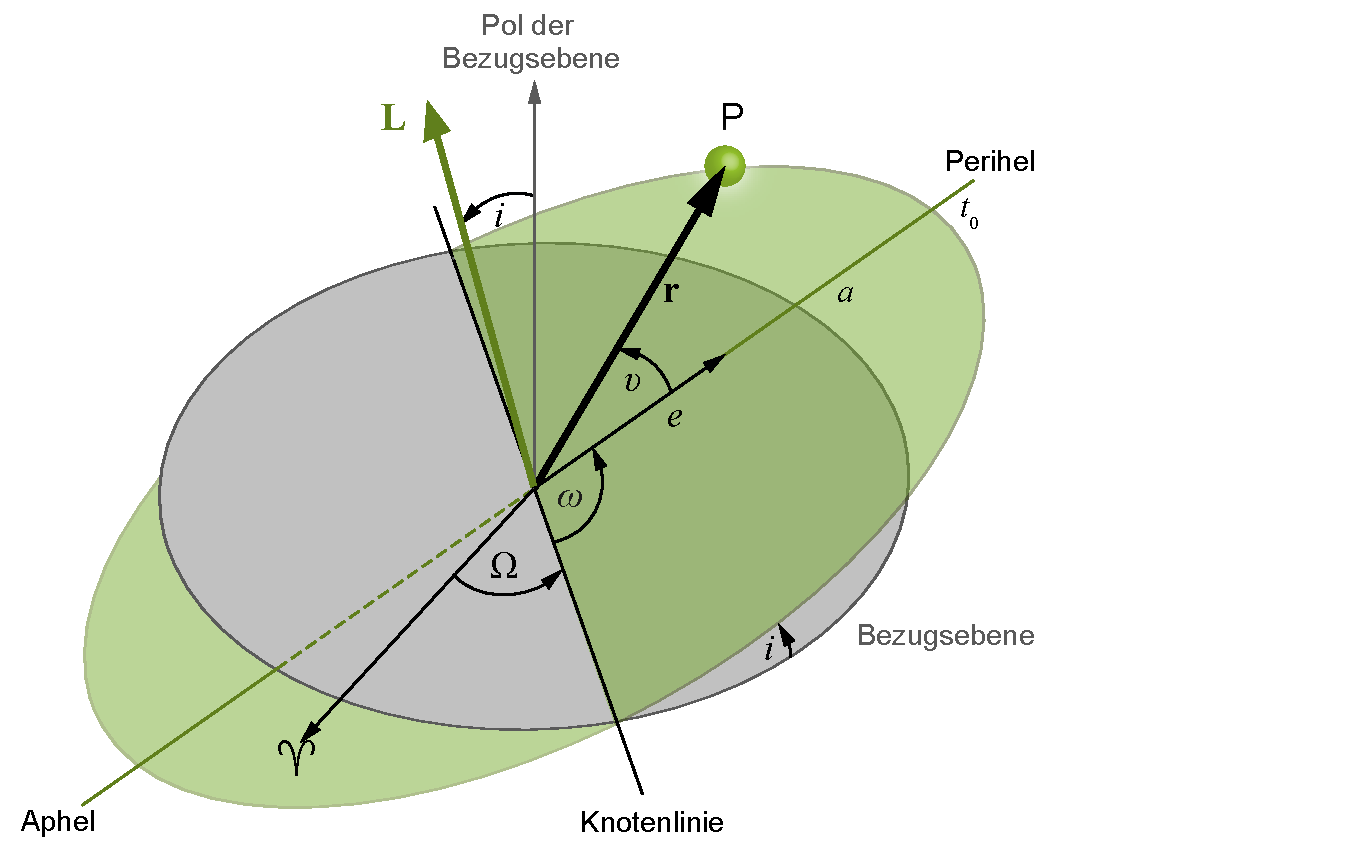
\includegraphics[width=\textwidth]{Bahnelemente2.pdf}%
\caption[Bahnelemente der Planeten im Sonnensystem.]{Bahnelemente der Planeten im Sonnensystem. $i$ bezeichnet die Inklination (Neigung der Bahn zur Ekliptik), $\Omega$ die L�nge des aufsteigenden Knotens, $\omega$ das Argument (den Winkel) des Perihels, $a$ die gro�e Halbachse, $e$ die Exzentrizit�t und $t_0$ die Periheldurchgangszeit. H�ufig wird auch die L�nge des Perihels $\varpi=\omega+\Omega$ angegeben.}
\label{abb:hm_bahnelemente}
\end{figure}

Bei Kenntnis der Bahnparameter\footnote{Man findet diese Bahnparameter an vielen Stellen, in astronomischen Jahrb�chern oder auch im Internet. Hier sei besonders auf die Seiten des \textit{\gls{jplhm}~(JPL)}\index{Jet Propulsion Lab (JPL)} auf \url{https://ssd.jpl.nasa.gov/?ephemerides} verwiesen.} im \glslink{ekliptkoord}{ekliptikalen System} kann man jederzeit mit den in Tabelle \ref{tab:hm_Umrechung_KOS} beschriebenen Transformationen die Bahnkoordinaten auch in jedem anderen KOS berechnen.\\
Wir sind aber nicht nur an der Form der Bahn, sondern insbesondere auch an dem zeitlichen Verlauf der Bewegung entlang der beschriebenen Bahn $r(\upsilon)$ interessiert, also an $r(t)$ bzw. an $\upsilon(t)$.
Die wahre Anomalie ist unserer Beobachtung wegen der gr��eren �nderung �ber die Zeit und einfacheren Messung von Winkeln relativ einfach zug�nglich.
Wir starten mit der Bahngeschwindigkeit in Polarkoordinaten
\begin{equation} \label{eq:hm_vis-viva_polar}
v^2 = \dot{r}^2 + r^2\dot{\upsilon}^2 = \dot{r}^2 + \frac{L^2}{r^2}  
\end{equation}
und setzen diesen Ausdruck in den vis-viva-Satz \eqref{eq:hm_vis-viva} ein.
Ebenso benutzen wir f�r $L$ die Beziehung \eqref{eq:hm_drehimpuls_von_ae} und erhalten  
\begin{align} \label{eq:hm_dot_r_quadrat} 
\dot{r}^2 &= \mu_\text{G} \lk \frac{2}{r} - \frac{1}{a} \rk - \frac{L^2}{r^2} = \mu_\text{G} \lk \frac{2}{r} - \frac{1}{a} - \frac{a(1-e^2)}{r^2} \rk \nonumber \\
					&= \frac{\mu_\text{G}}{r^2} \lk 2r - \frac{r^2}{a} - a\,(1-e^2) \rk\,.  
\end{align}
Jetzt f�hren wir die \gls{exzentranom} \index{Anomalie!exzentrische|textbf} $E(t)$ als Hilfsgr��e f�r die Berechnung von $r(t)$ ein: 
\begin{equation}
r(t) = a \,\lk 1-e\,\cos E(t)\rk \,.\label{eq:hm_exzentrische_Anomalie}
\end{equation}
Die mag zun�chst etwas formal-mathematisch erscheinen. Die geometrische Bedeutung von $E$ wird im \kapitel{deutung_kepler} klar werden.
Wir leiten \eqref{eq:hm_exzentrische_Anomalie} nach der Zeit ab
\begin{equation*}
\dot{r}(t) = \frac{\D r}{\D E} \frac{\D E}{\D t} = a\,e\,\sin E\, \frac{\D E}{\D t} \,,
\end{equation*}
setzen  dies in \eqref{eq:hm_dot_r_quadrat} ein und erhalten zun�chst
\begin{align*}
a^2\,e^2\,\sin^2 E \,\lk\frac{\D E}{\D t}\rk^2 &= \frac{\mu_\text{G}}{r^2} \,(a\,e^2 - a\,e^2\,\cos^2 E) = \frac{\mu_\text{G}}{r^2}\, a\,e^2 \,\sin^2 E\,. 
\end{align*}
Durch K�rzen von $a^2e^2\sin^2E$ und Wurzelziehen folgt
\begin{equation*}
r \lk \frac{\D E}{\D t} \rk = \sqrt{\frac{\mu_\text{G}}{a}} \,.%\label{eq:hm_r_dE_dt}
\end{equation*}
Mit der Definition der exzentrischen Anomalie \eqref{eq:hm_exzentrische_Anomalie} und Trennung der Variablen wird daraus
\begin{equation}
\lk 1-e\,\cos E(t) \rk \,\D E = \sqrt{\frac{\mu_\text{G}}{a^3}}\,\D t\,. \label{eq:hm_1-ecosEdE}
\end{equation}
Wir f�hren noch mit der Umlaufzeit $T_\text{P}$ \bzw der Umlaufwinkelgeschwindigkeit $n_\text{P}$ die \emph{mittlere Anomalie} $M$\glslink{mittlereanom} ein:
\begin{equation}
M = M(t) = \sqrt{\frac{\mu_\text{G}}{a^3}} \,(t-t_0) = \frac{2 \pi}{T_\text{P}}\,(t-t_0) = n_\text{P}\,(t-t_0) \,. \label{eq:hm_mittlere_anomalie}
\end{equation}
Nach Integration von \eqref{eq:hm_1-ecosEdE} �ber $\D E$ erhalten wir schlie�lich die ebenso ber�hmte wie kompakte \emph{Kepler-Gleichung}\index{Kepler-Gleichung}.
\begin{merksatz}{Kepler-Gleichung}
\begin{equation}
E-e\,\sin E = M  \,.\label{eq:hm_keplerglg}
\end{equation}\\

\end{merksatz}

Diese Gleichung wurde von Kepler\indexp{Kepler, Johannes} 1609 erstmals in seiner \anf{Astronomia Nova} \cite{Kepler1992} ver�ffentlicht.
Obwohl sie keine Differentialgleichung ist, handelt es sich tats�chlich um eine Bewegungsgleichung, denn auf beiden Seiten der Kepler-Gleichung stehen mit $M(t)$ und $E(t)$ zeitabh�ngige Gr��en.\footnote{Da wir Bewegungsintegrale bei der Herleitung von \eqref{eq:hm_keplerglg} verwendet haben, ist das Verschwinden der Ableitungen nach der Zeit nicht verwunderlich.
Eigentlich sollte man besser schreiben $E(t)-e\,\sin E(t)\!=\!M(t)$.} Die Bewegungsintegrale stecken in den (geometrischen) Parametern $e$ und $M$.
$M(t)$ ist durch die gro�e Halbachse $a$ oder nach dem 3.~Keplerschen Gesetz \eqref{eq:hm_3_kepler_gesetz} durch die Umlaufzeit $T_\text{P}$ gegeben.
Hat man �ber \eqref{eq:hm_keplerglg} $E(t)$ berechnet, kann man dann �ber \eqref{eq:hm_exzentrische_Anomalie} den Abstand $r(t)$ bzw. �ber \eqref{eq:hm_bahnglg} die wahre Anomalie $\upsilon(t)$ bestimmen. \\


\subsection{Geometrische Deutung und Ableitung der Kepler-Gleichung} \label{kap:deutung_kepler}

Wir wollen uns jetzt noch die Bedeutung der mittleren, wahren und exzentrischen \emph{Anomalien} anschaulich klar machen.
Dazu betrachten wir \figref{hm_geom_abl_kepler}.
Als \gls{fahrstrahl} wollen wir die Verbindungslinie zwischen dem gravitativen Schwerpunkt (\gls{gravizentrum}) des Systems -- hier in guter N�herung die Position des Zentralk�rpers -- und der Position des Planeten zum Zeitpunkt $t$ bezeichnen.

Dann ist die \textit{mittlere Anomalie} $M$\glslink{mittlereanom}\ der Winkel, der durch die \gls{apsidenlinie}\index{Apsidenlinie|textbf} (Verbindungslinie von \gls{periapsis} und \gls{apoapsis}) und den Fahrstrahl eines \anf{Quasiplaneten} Q gebildet wird. Q sei ein gedachter Quasiplanet, der mit konstanter Geschwindigkeit eine Kreisbahn mit Radius $a$ um das Ellipsenzentrum durchl�uft.\\
Die \textit{wahre Anomalie} $\upsilon$\glslink{wahreanomalie}\ ist durch den Winkel gegeben, den der Fahrstrahl des "`wahren"' Planeten P an der Position $r$ auf der Ellipse mit der Apsidenlinie bildet. Dieser Winkel ist identisch mit der Definition nach \figref{hm_ellipse}.
\begin{figure}
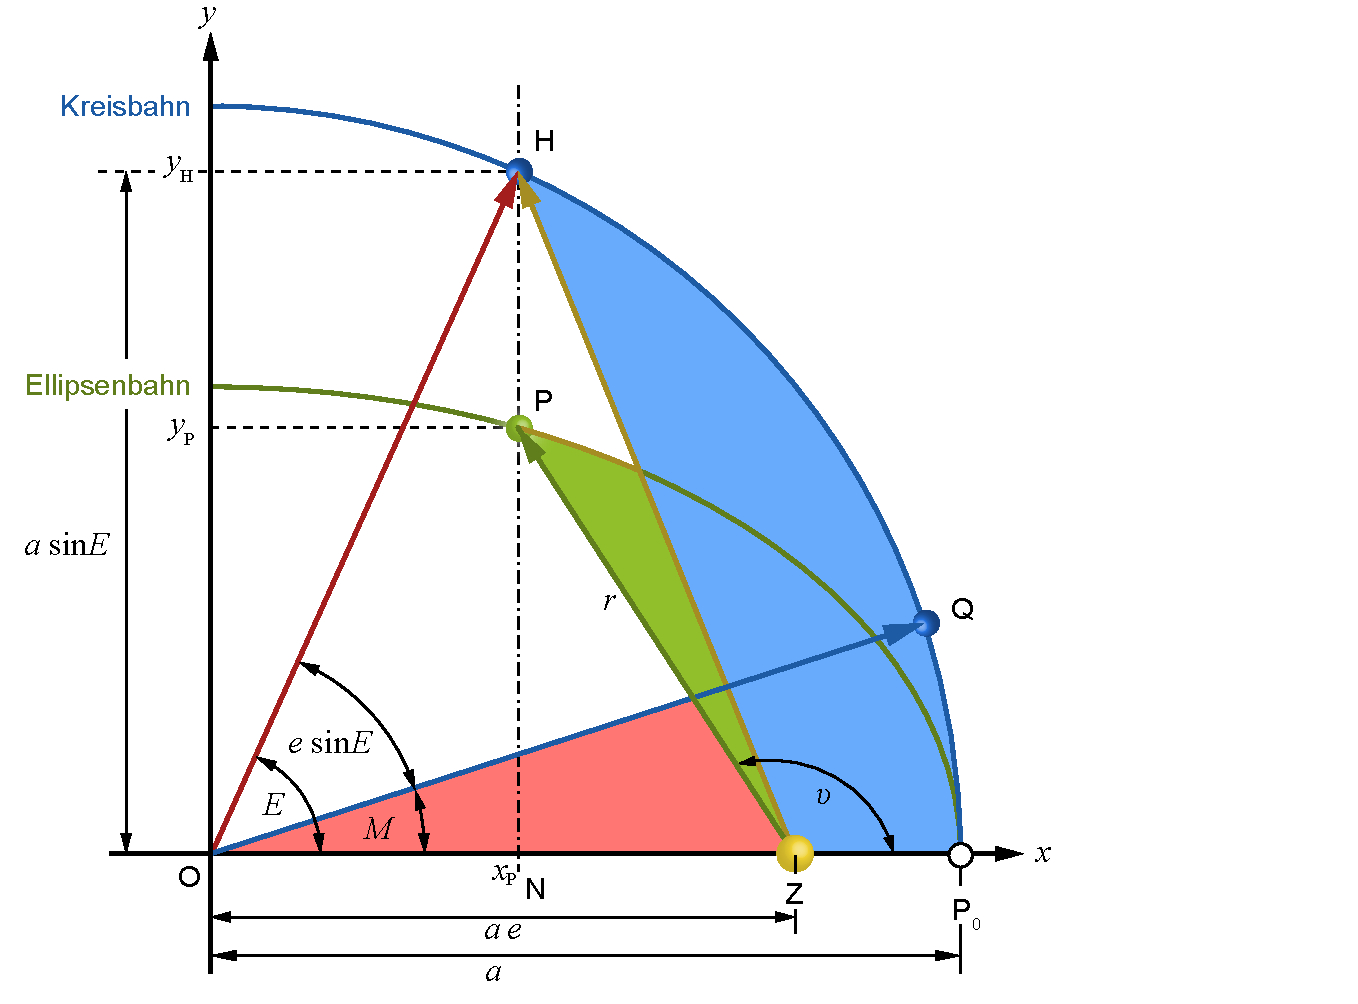
\includegraphics[width=\textwidth]{Geometrie_KG.pdf}
\caption[Geometrische Herleitung der Kepler-Gleichung.]{Geometrische Herleitung der Kepler-Gleichung. Bezeichnungen: P Planet, H "`Hilfsplanet"'"', Q "`Quasiplanet"', $\mathrm{P_0}$ Perihel (siehe Text).}
\label{abb:hm_geom_abl_kepler}
\end{figure}

Wir konstruieren uns einen weiteren Hilfsplaneten H, der dieselbe $x$-Position wie der Planet P hat und dessen $y$-Position sich aber aus der Projektion auf den Kreis mit dem Radius $a$ ergibt.
Den Winkel, der sich aus dem Fahrstrahl vom Kreis/Ellipsenzentrum O zum Hilfsplaneten H relativ zur Apsidenlinie ergibt, bezeichnen wir mit $E$.
Wir wollen zun�chst zeigen, dass der so definierte Winkel $E$ mit der nach \eqref{eq:hm_exzentrische_Anomalie} definierten \textit{exzentrischen Anomalie}\index{Anomalie!exzentrische} $E$ �bereinstimmt.
F�r die $x$-Koordinate $x_\text{P}(t)$ des Punktes $\text{P}(t)$ gilt einerseits
\begin{equation*}
x_\text{P}(t) = a\, e\, + r\,\cos \upsilon
\end{equation*}
und andererseits
\begin{equation*}
x_\text{P}(t) = a\,\cos E \,.
\end{equation*}
Gleichsetzen und Multiplikation mit $e$ ergibt
\begin{equation}
a\,e^2 + r\,e\,\cos \upsilon = a\,e\,\cos E \,. \label{eq:hm_ae_quadrat}
\end{equation}
Wir benutzen die Parameterdarstellung der Ellipse \eqref{eq:hm_bahnglg} in der Form 
	\[r\, e\,\cos \upsilon\!=\! a\,(1-e^2)-r\,,\]
die wir in \eqref{eq:hm_ae_quadrat} einsetzen.
Daraus folgt
\begin{equation}
r = a-a\,e\,\cos E = a\,(1-e\,\cos E) \,. \label{eq:hm_r_param_ellipse} 
\end{equation}
Damit ist die Gleichheit der nach \figref{hm_geom_abl_kepler} geometrisch definierten exzentrischen Anomalie $E$ mit der Definition \eqref{eq:hm_exzentrische_Anomalie} gezeigt.
Jetzt k�nnen wir unter Benutzung des Fl�chensatzes mit rein geometrischen �berlegungen die Kepler-Gleichung aus der Geometrie von \figref{hm_geom_abl_kepler} ableiten.\footnote{Diese Ableitung geht auf Kepler zur�ck und benutzt lediglich den empirisch gefundenen Fl�chensatz, denn 1609 war das Gravitationsgesetz ja noch nicht bekannt!}
Wir betrachten zun�chst die Kreisbogenfl�che $A_{\text{HOP}_0}(t)$.
Sie kann einerseits durch die Kreisbogenfl�che $A_{\text{HOP}_0}(t)\!=\! \pi a^2 E/2\pi \!=\!\lk a^2/2\rk\,E(t)$ (mit $E$ im Bogenma�) und andererseits als Summe der Dreiecksfl�che $A_\text{HOZ}$ und der krummlinigen Dreiecksfl�che $A_{\text{HZP}_0}(t)$ (blau gekennzeichnet) berechnet werden:
\begin{equation*}
A_{\text{HOP}_0}(t) = \frac{a^2}{2} E(t) = \frac{1}{2} a\,e\,a\,\sin E(t)+A_{\text{HZP}_0}(t)  \,.
\end{equation*}
Um eine Bestimmungsgleichung f�r $E(t)$ zu bekommen, m�ssen wir also $A_{\text{HZP}_0}(t)$ berechnen.
Dazu betrachten wir zun�chst die Streckenl�ngen $y_\text{H}\!=\!\overline{\text{NH}}$ und $y_\text{P}\!=\!\overline{\text{NP}}$.
Aus der Kreis- bzw. Ellipsengleichung folgt
\begin{align*}
y_\text{H} &= a \sqrt{1-\frac{\overline{\text{ON}}^2}{a^2}} ~~\text{bzw.} ~~y_\text{P} = b \sqrt{1-\frac{\overline{\text{ON}}^2}{a^2}} \,.
\end{align*}
Daraus folgt, dass sich die Fl�chen $A_\text{PZN}$ und $A_\text{HZN}$ der entsprechenden Dreiecke verhalten wie
\begin{equation}
\frac{A_\text{PZN}}{A_\text{HZN}} = \frac{\frac{1}{2} y_\text{P}\,\overline{\text{ZN}}}{\frac{1}{2} y_\text{H}\,\overline{\text{ZN}}} = \frac{b}{a} \,. \label{eq:hm_A_PZN_durch_A_HZN}
\end{equation}
F�r die Fl�chen der krummlinigen Dreiecke $A_{\text{PNP}_0}$ (Ellipsensegment) und $A_{\text{HNP}_0}$ (Kreissegment) sowie deren Verh�ltnis gilt
\begin{align*}
  A_{\text{PNP}_0} &= \, \int\limits_{a\cos E}^a\!b\sqrt{1-\frac{x^2}{a^2}} \,\D x \; \quad \text{und} \quad
  A_{\text{HNP}_0} = \, \int\limits_{a\cos E}^a\!a\sqrt{1-\frac{x^2}{a^2}} \,\D x \\
  \Rightarrow~~ &~~\frac{A_{\text{PNP}_0}}{A_{\text{HNP}_0}} = \frac{b}{a} \,.
\end{align*}
Da sich sowohl die Dreiecksfl�chen $A_\text{PZN}$ und $A_\text{HZN}$ als auch die krummlinigen Dreiecke $A_{\text{PNP}_0}$ und $A_{\text{HNP}_0}$ jeweils wie $b/a$ verhalten, muss dies auch f�r die Differenzfl�chen $A_{\text{PZP}_0}$ und $A_{\text{HZP}_0}$ gelten.
Damit ist
\begin{equation}
A_{\text{HZP}_0}(t) = \frac{a}{b}\,A_{\text{PZP}_0}(t) \,. \label{eq:hm_r_param_ellipse01} 
\end{equation}
Nun schauen wir uns noch das Verh�ltnis der Fl�che $A_\text{P}(t)\!=\!A_{\text{PZP}_0}$ zur Kreisbogenfl�che $A_\text{Q}(t)\!=\!A_{\text{QOP}_0}$ an.
Nach einem vollen Umlauf $T_\text{P}$ ist $A_\text{P}(T_\text{P})$ die Fl�che der Ellipse $\pi ab$ und $A_\text{Q}(T_\text{P})$ die Fl�che des Kreises $\pi a^2$.
Hier kommt der Fl�chensatz ins Spiel.
Nach diesem muss dieses Verh�ltnis auch f�r jeden beliebigen Zeitpunkt gelten, daher gilt
\begin{equation}
\frac{A_\text{P}(T_\text{P})}{A_\text{Q}(T_\text{P})} = \frac{\pi ab}{\pi a^2} = \frac{A_\text{P}(t)}{A_\text{Q}(t)} = \frac{A_{\text{PZP}_0}}{A_{\text{QOP}_0}} = \frac{b}{a} \,.\label{eq:hm_F_P_durch_F_Q}
\end{equation}
Mit \eqref{eq:hm_r_param_ellipse01} folgt sofort
\begin{equation*}
A_{\text{HZP}_0} = \frac{a}{b} A_{\text{PZP}_0} = \frac{ab}{ba} A_{\text{QOP}_0} = A_{\text{QOP}_0} = \frac{M}{2}a^2 = \frac{a^2}{2}\frac{2\pi}{T_\text{P}}\,(t-t_0) \,.
\end{equation*}
Eingesetzt in die oben gefundene Aufteilung der Fl�che folgt daraus
\begin{equation*}
\frac{a^2}{2}\,E(t) = \frac{1}{2}a\,e\,a\,\sin E(t) + \frac{a^2}{2} M(t)\; ,
\end{equation*}
woraus sich mittels Division durch $a^2/2$ die Kepler-Gleichung ergibt.\\

Wir wollen zum Schluss noch eine n�tzliche Formel f�r $\upsilon(t)$ angeben:
\begin{equation}
\tan \lk \frac{\upsilon}{2} \rk = \sqrt{\frac{1+e}{1-e}}\,\tan\lk\frac{E}{2}\rk\,. \label{eq:hm_nu(t)_alternativ}
\end{equation}
Diese l�sst sich ebenfalls aus der Geometrie der \figref{hm_geom_abl_kepler} herleiten, indem man den Kosinus der wahren Anomalie durch die exzentrische Anomalie ausdr�ckt und die trigonometrische Beziehung f�r den halben Winkel verwendet (\probref{hm_wahre_anomalie}).
�hnliche Bewegungsgleichungen, wie wir sie hier f�r die Ellipse gezeigt haben, k�nnen auch f�r die Parabel und die Hyperbel hergeleitet werden (\probref{hm_bwglg_hyp_parab}).

Jetzt m�ssen wir nur noch die Kepler-Gleichung l�sen. Das hat es aber durchaus in sich.



\section{L�sung der Kepler-Gleichung} \label{kap:lsg_kepler}

Das Besondere an der Kepler-Gleichung ist neben ihrer grundlegenden Bedeutung f�r die Himmelsmechanik ihre offensichtliche Einfachheit und Kompaktheit in der Formulierung (man kann auch sagen Sch�nheit) und ihre gleichzeitige Komplexit�t in der L�sung. Schon Kepler wies darauf hin, dass er f�r die Gleichung keine analytisch geschlossene L�sung finden konnte und stachelte nachfolgende Generationen an, sich der L�sung dieser Aufgabe zu widmen \cite{Kepler1992}.
Neben Newton\indexp{Newton, Sir Isaac}  waren es vor allem Lagrange\footnote{Joseph-Louis Lagrange (1736--1813) war ein italienisch-franz�sischer Mathematiker und Astronom und gilt als Begr�nder der analytischen Mechanik (\emph{M�canique Analytique}, 1788).}\indexp{Lagrange, Joseph-Louis}, Cauchy\footnote{Augustin-Louis Cauchy (1789--1857) war ein franz�sischer Mathematiker, der besonders auf dem Gebiet der Analysis t�tig war.}\indexp{Cauchy, Augustin-Louis} und Bessel\footnote{Friedrich Wilhelm Bessel (1784--1846) war ein deutscher Wissenschaftler, der auf den Gebieten der Astronomie, Mathematik, Geod�sie und Physik bedeutsame Beitr�ge lieferte.}\indexp{Bessel, Friedrich Wilhelm}, die sich dem Thema widmeten und aus der Besch�ftigung mit der Kepler-Gleichung wertvolle und fundamentale Beitr�ge zur Entwicklung der Mathematik lieferten.
Erw�hnt seien die Newton-Raphson-N�herungsmethode, inverse Reihenentwicklungen, komplexe Analysis und die Bessel-Funktionen.
Seither gab es in jeder Dekade mindestens ein oder zwei Arbeiten zur analytisch geschlossenen L�sung der Kepler-Gleichung.
Als aktuelle Beispiele seien die Arbeiten in \cite{Siewert1972} und \cite{Perovich2016} angef�hrt.
Sie reihen sich ein in das Bem�hen, weiter nach einer einfachen analytisch geschlossenen L�sung (zumindest f�r Spezialf�lle) zu suchen.
Wir wollen im Folgenden jedoch die beiden grunds�tzlichen N�herungsmethoden (Iteration und Reihenentwicklung) zur L�sung der Kepler-Gleichung vorstellen.             

\subsection{Iterationsverfahren}\index{Iterationsverfahren} \label{kap:iteration_kepler}
Ein naheliegender Ansatz zur L�sung der Kepler-Gleichung ist die Iteration\index{Iteration}, d.\,h. man berechnet eine N�herung f�r die Gr��e $E_{k+1}(t)$ aus einer zuvor bestimmten N�herung $E_k(t)$ nach
\begin{equation*}
E_{k+1}(t) = M(t) + e\,\sin E_k(t) 
\end{equation*}
mit dem sinnvollerweise zu setzenden \textit{Iterationsanfang}
\begin{equation}
E_0 (t)=M(t) ~.\label{eq:hm_iteration_anfang}
\end{equation}
Das liegt besonders nahe, wenn die Exzentrizit�t $e$ relativ klein ist, weil dann die Abweichung von der Kreisbahn relativ gering ist.
Man kann aber auch andere Iterationsanf�nge w�hlen und in bestimmten F�llen muss man das auch, insbesondere bei gro�en Exzentrizit�ten $e$ \cite{Strebel2001}.
Unter Nutzung der trigonometrischen Additionstheoreme $\sin(x+y)\!=\!\sin x \cos y + \cos x \sin y$ und der N�herung f�r kleine Argumente $\sin x\!\approx\! x -  x^3/6 + \ldots$ bzw. $\cos x\!\approx\! 1-x^2/2 + \ldots$ kann auf \eqref{eq:hm_iteration_anfang} folgend die n�chste Iteration durchgef�hrt werden:\footnote{Wir lassen der Einfachheit halber die Notation der Zeit $t$ weg.}
\begin{equation}
E_1 = M+e\,\sin M ~~. \label{eq:hm_E_1_kepler}
\end{equation}
Der n�chste \textit{Iterationsschritt} lautet:
\begin{align}
\begin{split}
E_2 &= M + e\,\sin E_1 = M + e\,\sin (\underbrace{M+e\,\sin M}_{E_1}) \\
		&= M + e\,\sin M\, \cos(\underbrace{e\,\sin M}_{E_1-E_0})  +  e\,\cos M\, \sin(\underbrace{e\,\sin M}_{E_1-E_0}) \,. 
\end{split} \label{eq:hm_E_2_kepler}
\end{align}
Da $E_{k+1}(t)-E_k(t)\!=\!e\,\sin E_k(t)$ eine kleine Gr��e ist, kann man mit der N�herung f�r kleine Winkel schreiben:
\begin{align*}
E_2 &\approx  M + e\,\sin M\, \lk 1-\frac{e^2}{2} \sin^2 M \rk + e\,\cos M \, e\,\sin M + \mathcal{O}(e^3) \\
    &= M + e\,\sin M + \frac{e^2}{2}\,\sin 2M + \mathcal{O}(e^3) \,. 
\end{align*}
Der n�chste Iterationsschritt ergibt
\begin{equation*}
E_3 \approx M + e\,\sin E_2 = M+e\sin\lk M+e\sin M+\frac{1}{2}e^2 \sin 2M\rk ~~, \label{eq:hm_E_3_kepler}
\end{equation*}
woraus wiederum mit den Additionstheoremen und N�herungen f�r kleine $e$ folgt:
\begin{equation*}
E_3 = M+ \lk e-\frac{1}{8} e^3\rk \sin M + \frac{1}{2}e^2\,\sin 2M + \frac{3}{8}e^3\,\sin 3M + \mathcal{O}(e^4) \,.
\end{equation*}
Verallgemeinert man die Schritte induktiv, erh�lt man
\begin{equation}
E = M+ \sum_{k=1}^{\infty} b_k(e)\,\sin kM \,. \label{eq:hm_reihenentw_iteration}
\end{equation}
Diese Reihe stellt eine Entwicklung nach \anf{Frequenzvielfachen} von $M$ dar.
Das kann auch so verstanden werden, dass die Zeitentwicklung der Bewegung auf der Ellipsenbahn gegen�ber der reinen Kreisbahnbewegung Oberfrequenzen hat, deren Koeffizienten von der Exzentrizit�t $e$ abh�ngen.
Im Fall von $e\!>\!0.6627434$ divergiert die Entwicklung nach \eqref{eq:hm_reihenentw_iteration} \cite{Murray2008}.
Es muss dann auf andere Iterationsverfahren (Regula falsi, Newton-Raphson, Sekanten- und Tangentenverfahren) und andere Iterationsstartwerte zur�ckgegriffen werden \cite{Strebel2001}.
Wir geben hier noch die Entwicklung von \eqref{eq:hm_reihenentw_iteration} bis zur vierten Ordnung von $e$ an:
\begin{align}
\begin{split}
E = M &+\lk e-\frac{1}{8}e^3\rk \sin M + \lk \frac{1}{2} e^2 - \frac{1}{6} e^4 \rk \sin 2M  \\
      &+ \frac{3}{8}e^3\,\sin 3M + \frac{1}{3} e^4\,\sin 4M + \mathcal{O}(e^5) \,. 
\end{split} \label{eq:hm_entwicklung_4Ord}
\end{align}
Damit haben wir eine N�herungsl�sung f�r $E$ gewonnen, aus der man �ber \eqref{eq:hm_nu(t)_alternativ} die wahre Anomalie des Planeten \bzw �ber \eqref{eq:hm_exzentrische_Anomalie} dessen Entfernung zum Zentralk�rper bestimmen kann.
Die L�sung beinhaltet als Parameter lediglich die Exzentrizit�t $e$ und �ber $M$ die gro�e Halbachse $a$ und die Zeitdifferenz zum Anfangswert $t_0$.
Die Frage ist nun, ob die Koeffizienten $b_k(e)$ in \eqref{eq:hm_reihenentw_iteration} in einer allgemeinen Form dargestellt und nicht nur schrittweise �ber ein Iterationsverfahren berechnet werden k�nnen.

\subsection{Reihenentwicklung}\index{Reihenentwicklung}
Da $E\!-\!M\!=\!e\sin E$ f�r kleine $e$ eine kleine Gr��e ist, ist es sinnvoll, die Kepler-Gleichung nach $E\!-\!M$ zu entwickeln.
Wir machen dazu folgenden Ansatz:
\begin{align*}
e\,\sin E &= \sum_{k=1}^{\infty} b_k(e)\,\sin(kM) \Rightarrow b_k(e) = \frac{2}{\pi} \int\limits_0^\pi e\,\sin E\,\sin(kM) \,\D M \,. 
\end{align*}
Mittels partieller Integration unter Nutzung der Kepler-Gleichung ergibt sich
\begin{align*}
b_k(e) &= \underbrace{\frac{2}{k\pi} \lek e\,\sin E\,\cos(kM) \rek^0_\pi}_{=0} + \frac{2}{k\pi} \int\limits_0^\pi \lk \frac{\D E}{\D M} -1\rk \cos(kM)\,\D M \\
       &= \frac{2}{k\pi} \int\limits_0^\pi \cos (kM) \,\D E - \underbrace{\frac{2}{k\pi} \int\limits_0^\pi \cos (kM) \D M}_{=0} \,. 
\end{align*}
Setzen wir $kM =  k\,\lk E - \sin E \rk$ (Kepler-Gleichung) im Integranden, erhalten wir
\begin{equation}
b_k(e) = \frac{2}{k\pi} \int\limits_0^\pi \cos \lek k(E-e\,\sin E)\rek \,\D E \,. \label{eq:hm_b_k(e)}
\end{equation}
Hier verwenden wir jetzt die \emph{Bessel-Funktionen} erster Art $\mathcal{J}_n (z)$, die �ber das \emph{Bessel-Integral} wie folgt definiert \cite{Olver1992} sind:
\begin{align}
  \mathcal{J}_n(z)
  &= \frac{1}{\pi} \int\limits_0^\pi \cos (z\,\sin\theta - n\theta)\,\D \theta 
    = \frac{1}{n!} \lk \frac{z}{2} \rk^n \sum_m^{\infty} (-1)^m \frac{(z/2)^{2m}}
    {m! (n+1)(n+2) \ldots (n+m)} \,.\label{eq:hm_besselfkt_erster_art_int}
\end{align}
Da die cos-Funktion gerade ist, kann \eqref{eq:hm_b_k(e)} mit \eqref{eq:hm_besselfkt_erster_art_int} geschrieben werden als
\begin{equation}
b_k(e) = \frac{2}{k} \mathcal{J}_k(ke) \,. \label{eq:hm_b_k(e)_Bessel}
\end{equation}
Damit l�sst sich die L�sung der Kepler-Gleichung nun als Reihe mit \gls{besselfkt}en schreiben:
\begin{equation}
E = M + 2 \sum_{k=1}^\infty \frac{\mathcal{J}_k(ke)}{k}\,\sin(kM) \,.
\label{eq:hm_lsg_kepler_reihe}
\end{equation}
Wir empfehlen die Reihenentwicklung \eqref{eq:hm_lsg_kepler_reihe} einmal selbst bis zur vierten Ordnung in $e$ durchzuf�hren.
Als Ergebnis erh�lt man eine der Reihe \eqref{eq:hm_entwicklung_4Ord} entsprechenden L�sung.
Numerische Berechnungen zur Konvergenz der Reihe 
\eqref{eq:hm_lsg_kepler_reihe} sind in \probref{hm_bessel} ausgef�hrt.


\subsection{Mittelpunktsgleichung}\label{kap:hm_mpg}
Da \glslink{mittelpunktsglg} bei kleinen Exzentrizit�ten auch die Differenz von wahrer und mittlerer Anomalie eine kleine Gr��e sein sollte, ist f�r viele Problemstellungen eine Reihenentwicklung dieser Differenz direkter und besser geeignet.
Man spart sich dabei den Zwischenschritt der Berechnung von $E$ und die anschlie�ende Umrechnung in $\upsilon$ �ber \eqref{eq:hm_nu(t)_alternativ}.
Eine solche Reihenentwicklung f�r die Differenz von wahrer und mittlerer Anomalie wird auch Mittelpunktsgleichung genannt:
\begin{infobox} {Mittelpunktsgleichung}
\begin{align}
\begin{split}
\mathcal{C}=\upsilon-M &= 2e \sin M + \frac{5}{4}e^2\,\sin(2M) \\
&+ e^3 \lk \frac{13}{12} \sin(3M) - \frac{1}{4} \sin M \rk  \\
&+ e^4 \lk \frac{103}{96} \sin(4M) - \frac{11}{24} \sin(2M)  \rk + \mathcal{O}(e^5) \,. 
\end{split} \label{eq:hm_mpglg_nu-M}
\end{align} \\
\end{infobox}

Da wir die Mittelpunktsgleichung im Folgenden h�ufig brauchen werden, zeigen wir die Herleitung dieser Reihe in Beispiel \ref{bsp:mittelpktglg} und einen alternativen Weg in \probref{hm_alternative_MPG}.
Ebenso kann in �hnlicher Form eine Reihe f�r $r/a$ abgeleitet werden (siehe dazu auch \cite{Brouwer1961,Guthmann2000}):
\begin{align}
\begin{split}
\frac{r}{a} = &1 + \frac{1}{2}e^2 - 2e \sum_k^\infty \frac{1}{k^2} \frac{\D }{\D e} \mathcal{J}_k(ke)\,\cos(kM) \\
            = &1-e \cos M + e^2(1-\cos(2M) + \frac{3}{8}e^3 (\cos M - \cos(3M)  \\
						&+\frac{1}{3} e^4 (\cos(2M) - \cos(4M) + \mathcal{O}(e^5) \,.  
\end{split} \label{eq:hm_mpglg_r/a}
\end{align}

%BEISPIEL 3 %%%%%%%%%%%%%%%%%%%%%%%%%%%%%%%%%%%%%%%%%%%%%%%%%%%%%%%%%%%%%%%%%%%%%%%%%%%%%%%%%%
\begin{example}{Mittelpunktsgleichung}
\textit{Wir wollen die Mittelpunktsgleichung herleiten. Wir starten mit der Beziehung \eqref{eq:hm_drehimpuls_von_ae} f�r den Drehimpuls $r(\upsilon)$ und leiten daraus eine Gleichung f�r $\dot{\upsilon}(r)$ ab, die wir mit $\text{d}M\!=\!2\pi/T_\text{P}\,\text{d}t$ und der Substitution $r$ mittels der Definition der exzentrischen Anomalie in eine Gleichung f�r $\text{d}\upsilon\!=\!f(\text{d}M)$ umformen. Diese Gleichung
enth�lt $\text{d}E/\text{d}M$. F�r $\text{d}E/\text{d}M$ setzen wir die Bessel-Reihe \eqref{eq:hm_lsg_kepler_reihe} ein und k�nnen das Zwischenergebnis dann gliedweise integrieren.}\\

Wir starten also mit der Beziehung f�r den Drehimpuls nach \eqref{eq:hm_drehimpuls_von_ae} und nutzen das 3.~ Keplersche Gesetz:
\begin{align*}
L &= \sqrt{a\mu_\text{G}(1-e^2)} = r^2\,\dot{\upsilon} = \sqrt{1-e^2}\,n_\text{P}\,a^2\,.
\end{align*}
Mit der Definition der exzentrischen Anomalie $r\!=\!a(1-e\cos E)$ k�nnen wir schreiben:
\begin{align}
a^2(1-e\cos E)^2\,\text{d}\upsilon &= n_\text{P}\,a^2\sqrt{1-e^2}\,\text{d}t \nonumber \\
\Rightarrow \text{d}\upsilon &= \frac{\sqrt{1-e^2}}{(1-e\cos E)^2}\,\text{d}M ~~\text{mit}~~ \text{d}t = \frac{1}{n_\text{P}}\,\text{d}M \label{eq:hm_bsp_mpg_9} \,.
\end{align}
Differentiation der Kepler-Gleichung nach $\text{d}M$ ergibt die Beziehung:
\begin{align*}
\frac{\text{d}}{\text{d}M} E &= \frac{\text{d}}{\text{d}M} (M+e\sin E) = 1+e\cos E \frac{\text{d}E}{\text{d}M} ~~\Rightarrow \frac{\text{d}E}{\text{d}M} = \frac{1}{1-e\cos E} \,,
\end{align*}
die wir  in \eqref{eq:hm_bsp_mpg_9} einsetzen und
\begin{equation}
\text{d}\upsilon = \sqrt{1-e^2} \lk \frac{\text{d}E}{\text{d}M} \rk^2 \text{d}M \, \label{eq:hm_bsp_mpg_10}
\end{equation}
erhalten. Das ist schon eine differentielle Form von $\upsilon(M)$, die wir aber noch integrieren m�ssen. 
Um eine integrierbare Form f�r $\text{d}E/\text{d}M$ zu erhalten, leiten wir die Bessel-Reihe \eqref{eq:hm_lsg_kepler_reihe} nach $\text{d}M$ ab:
\begin{align*}
\frac{\text{d}E}{\text{d}M} &= \frac{\text{d}}{\text{d}M} \lk M + 2 \sum_{k=1} \frac{\mathcal{J}_k(ke)}{k}\,\sin(kM) \rk = 1+ 2 \sum_{k=1}\,{\mathcal{J}_k(ke)}\,\cos(kM) \\
                            &= \frac{\text{d}}{\text{d}M} \lk M + e\sin M + \frac{e^2}{2}\sin(2M) + \ldots \rk = 1+e\cos M + e^2\cos(2M) + \mathcal{O}(e^3) ~.
\end{align*}
Hierbei haben wir die Entwicklung der Bessel-Funktion \eqref{eq:hm_besselfkt_erster_art_int} nur bis zum quadratischen Term ber�cksichtigt.
Quadrieren ergibt:
\begin{align*}
\lk\frac{\text{d}E}{\text{d}M}\rk^2 &= [ 1+ \underbrace{e\cos M}_{=x} + \underbrace{e^2\cos(2M)}_{=y} + \:\mathcal{O}(e^3)]^2 \,.
\end{align*} 
Mit der Zwischenrechnung $(1+x+y+\ldots)(1+x+y+\ldots)\!=\!1+2x+2y+2xy+x^2+y^2+\ldots\!=\!1+2x+(2y+x^2)+2xy+\ldots$ erhalten wir zun�chst
\begin{align*}
\lk\frac{\text{d}E}{\text{d}M}\rk^2 &= 1+2e\cos M + 2e^2\cos(2M) + \underbrace{e^2\cos^2 M}_{=\frac{e^2}{2}(1+\cos(2M))} + 2e^3\cos M\cos(2M) \\
&= 1+2e\cos M + \frac{1}{2}e^2 + \frac{5}{2} e^2\cos(2M) + 2e^3\cos M\cos(2M)
\end{align*}
und damit �ber Integration von \eqref{eq:hm_bsp_mpg_10} schlie�lich
\begin{align}
\begin{split}
\upsilon &= \lk M + 2e\sin M + \frac{5}{4} e^2\sin(2M) + \frac{1}{2} e^2 M \rk \lk 1-\frac{1}{2} e^2+\ldots \rk \\ 
\upsilon &= M + 2e\sin M + \frac{5}{4}e^2\sin(2M) + \mathcal{O}(e^3) \,. 
\end{split}\label{eq:hm_bsp_mpg_12}
\end{align}
Wir empfehlen in den \textbf{�bungen} \ref{prob:hm_iteration} und \ref{prob:hm_bessel} die Entwicklung  von \eqref{eq:hm_bsp_mpg_12} bis zu Ordnungen $\mathcal{O}(\geq e^4)$ auszuf�hren.
Man kann dazu auch die Symbolic Math Toolbox von \matlab{} oder �hnliche Tools nutzen.\\

\label{bsp:mittelpktglg}
\end{example}
%BEISPIEL %%%%%%%%%%%%%%%%%%%%%%%%%%%%%%%%%%%%%%%%%%%%%%%%%%%%%%%%%%%%%%%%%%%%%%%%%%%%%%%%%%

Mit der nun vorliegenden L�sung der Kepler-Gleichung wollen wir uns erst einmal auf das System Sonne-Erde konzentrieren, um anschlie�end auch Bahnen von Planeten und Kometen zu berechnen.





\section{Himmelsmechanik unseres Sonnensystems}\label{kap:hm_keplergleichung}

\subsection{Erdbahn (Ekliptik)}\index{Erdbahn} \label{kap:erdbahn}
Wegen der besonderen Bedeutung der Erdbahn (Ekliptik) \glslink{ekliptik} bzw. der scheinbaren \anf{Sonnenbahn}\index{Sonnenbahn!scheinbare} (im geozentrischen System) f�r viele Himmelsph�nomene wollen wir uns mit der Erdbahn etwas n�her besch�ftigen.
Sie wird in guter N�herung durch eine Keplerellipse beschrieben, deren geringe numerische Exzentrizit�t $e\!\approx\!0.0167$ die Bahn nur relativ wenig von einer Kreisbahn abweichen l�sst.
Einige Bahnparameter hatten wir bereits eingef�hrt (Tabelle \ref{tab:hm_bahnparameter}).
Die gro�e Halbachse $a = a_\text{\earth}$ der Erdbahn betr�gt etwa 149.6 Millionen Kilometer, woraus sich �ber den mittleren Abstand der Erde von der Sonne die \gls{ae} AE ergibt.
Im zeitlichen Mittel betr�gt der Abstand zwischen Erde und Sonne etwas mehr als eine AE (n�mlich $1.00014\:\text{AE}$), da sich die Erde wegen ihrer ungleichf�rmigen Bahngeschwindigkeit etwas l�nger in Sonnenferne aufh�lt als in Sonnenn�he (\probref{hm_erdbahn_im_jahr}). 

Wir m�ssen an dieser Stelle noch eine Bemerkung zum Abstand zwischen Sonne (\astrosun) und Erde (\earth) machen: Wegen der gro�en Massenverh�ltnisse $m_\text{\astrosun} \gg m_\text{\earth}$ ist das ZKP effektiv ein Eink�rperproblem, \dh in guter N�herung bewegt sich die Erde um die \anf{ruhende} Sonne.
Nun hat die Erde ja aber einen durchaus massereichen Mond (\leftmoon).
Daher bewegt sich nicht der Erdmittelpunkt auf der Kepler-Ellipse um die Sonne, sondern der gemeinsame Schwerpunkt von Mond und Erde.
Dieser Schwerpunkt liegt im Erdinneren \ca $\SI{4000}{\kilo\metre}$ vom Erdmittelpunkt entfernt.
Der Erdmittelpunkt selbst kreist um diesen Schwerpunkt und vollf�hrt folglich eine Art Schlangenlinie entlang der Ellipsenbahn mit einer Periode entsprechend der Umlaufzeit des Mondes um die Erde.
Wenn wir im Folgenden von der \anf{Erdbahn} sprechen, ist in der Regel die gleichm��ige Ellipsenbahn des Erde-Mond-Schwerpunkts gemeint.
Bei Angabe von Zeitpunkten, in denen bestimmte Bahnpunkte durchlaufen werden (\zb das Perihel), ist daher zu unterscheiden, ob sich die Angaben auf den Erde-Mond-Schwerpunkt oder auf den Erdmittelpunkt beziehen (siehe auch Tabelle \ref{tab:hm_bahnparameter} im Tabellenanhang).

F�r die Berechnung der Bahn als Funktion der Zeit messen wir die Zeit in Bruchteilen von Julianischen Jahrhunderten, die seit dem Zeitpunkt J\,2000 $=$ 01.\,01.\,2000, 12:00 UT $=$ 2451545.0 vergangen sind.
Wir benutzen dann anstelle von $T$ (in Julianischen Tagen) zur besseren Unterscheidung die Bezeichnung $t$ f�r (vergangene) Julianische Jahrhunderte:
\begin{equation}
t = \frac{T-\text{J\,2000}}{36525} = \frac{T- 2451545.0}{36525} = \frac{\text{MJD}-51544.5}{36525}~.\\
\label{eq:hm_julian_centuries}
\end{equation}

\begin{figure}%
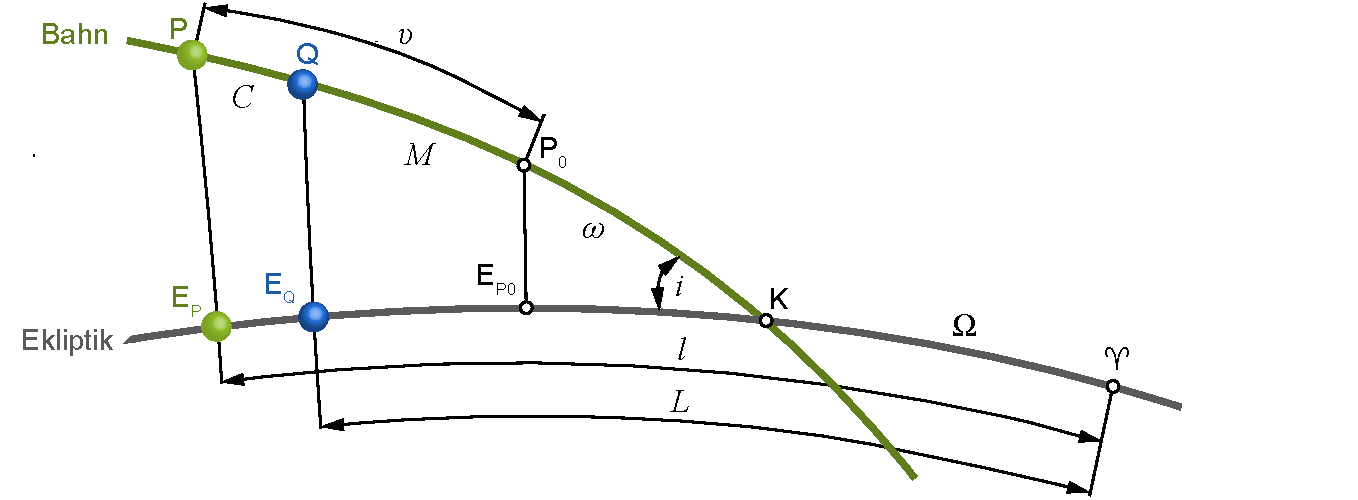
\includegraphics[width=\textwidth]{Bahn_Ekliptik.pdf}%
\caption[Verlauf einer Planetenbahn relativ zur Ekliptik.]{Verlauf einer Planetenbahn relativ zur Ekliptik. Gezeigt ist die Bahn eines Planeten P in der N�he des Fr�hlingspunktes $\vernal$ und des aufsteigenden Knotens K. Dieser ist bei der Erdbahn nicht definiert. Deswegen wird der Fr�hlingspunkt $\vernal$ als Bezugspunkt der Bahngleichung genommen (mathematisch gleichbedeutend mit $\Omega=0$). $\text{P}_0$ bezeichnet das Perihel, $\text{E}_\text{P}$ die Projektion des Planeten P auf die Ekliptik und $\text{E}_\text{Q}$  die Projektion des Hilfsplaneten Q. Dieser entspricht quasi einem auf der Kreisbahn mit der entsprechenden mittleren Anomalie $M$ sich mit konstanter Geschwindigkeit bewegenden \anf{mittleren} Planeten.}
\label{abb:hm_planetenbahnen_rel_ekliptik}
\end{figure}

Um die Position der Erde relativ zur Sonne \bzw sp�ter eines beliebigen Planeten als Funktion der Zeit zu berechnen, betrachten wir \figref{hm_planetenbahnen_rel_ekliptik}.
Wir schauen quasi von der Sonne in der Ekliptik-Ebene auf die Bahn des Planeten in Richtung des aufsteigenden Knotens\glslink{aufstknoten}\ K,
und haben auch den Fr�hlingspunkt $\vernal$ ins Blickfeld gelegt.\footnote{Die Abbildung entspricht der Darstellung \ref{abb:hm_bahnelemente}, aber aus einer anderen Perspektive.}\\
F�r die Erde vereinfacht sich das Bild erheblich, da $i\!=\!0$ und $\Omega\!=\!0$ (�quinoktium des Datums).
Wir k�nnen zun�chst relativ einfache Formeln f�r die heliozentrisch-ekliptikale L�nge der Erde $l_\text{\earth}$ (siehe \ref{tab:hm_astro_KOS}) gewinnen: 
\begin{align} 
\begin{split}
l_\text{\earth} &= \upsilon + \omega + \Omega\ = \upsilon + \varpi = (\upsilon-M)+M+\varpi \\
                &= \mathcal{C} + M + \varpi \,, 
\end{split} \label{eq:hm_ekl_laenge_erde1}
\end{align}
worin $\mathcal{C}\!=\!\upsilon-M$ die \gls{mittelpunktsglg} \eqref{eq:hm_mpglg_nu-M} ist.
F�r die heliozentrische Breite der Erde gilt $b_\text{\earth}\!=\!0$.
Wir wollen die Zeitabh�ngigkeit explizit ausdr�cken und w�hlen als Zeitreferenzpunkt die Epoche $t_\text{E}$ (\zb J2000).
\begin{align} 
l_\text{\earth} &= \mathcal{C}(t-t_\text{E}) + M(t-t_\text{E}) + \varpi_0 + \dot\varpi (t-t_\text{E}) \,, \label{eq:hm_ekl_laenge_erde2}
\end{align}
worin $\varpi_0 = \varpi(t_\text{E})$ ist und wir den linearen Term in der zeitlichen Entwicklung von $\varpi$ explizit mitgenommen haben (entsprechend Tabelle \ref{tab:hm_zeitl_aenderung_bahnparameter_lin}).
Dieser Term repr�sentiert die bereits erw�hnte Verschiebung des Fr�hlingspunktes durch die Pr�zession der Erdachse.
Wir schreiben die mittlere Anomalie $M(t)$ nach \eqref{eq:hm_mittlere_anomalie} als:
\begin{equation}
M(t-t_\text{E}) = n_\text{anom} \cdot (t-t_\text{E}) = n_\text{anom}\,t + M_0 \\
\label{eq:hm_mittlere_anomalie_ansatz}
\end{equation}
mit $M_0\!=\!357.5256\degree$ und $n_\text{anom}\!=\! 360\degree \cdot 36525/T_\text{anom}\!=\!35999.0498\,\degree/\text{Jh.}$ (\cite{Meeus1998,Montenbruck2001,Montenbruck1999} und Tabelle \ref{tab:hm_bahnparameter}).
Hierin ist $T_\text{anom}\!=\!365.259636\: \text{d}$ das \glslink{anomjahr}{anomalistische Jahr}\index{Jahr!anomalistisches}, also die Zeit zwischen zwei Durchg�ngen der Erde durch das Perihel.\\
Andererseits ist die \emph{mittlere L�nge} $L_\text{\earth}(t)$ der Erde definiert als die ekliptikale L�nge einer mit konstanter Umlaufgeschwindigkeit $n_\text{trop}$ (gegeben durch die Umlaufzeit eines tropischen Jahres) auf einer Kreisbahn umlaufenden \emph{mittleren Erde} (siehe Definition des tropischen Jahres in \kapitel{hm_zeitdefinition}), also
\begin{equation}
L_\text{\earth}(t) = n_\text{trop}\,t + L_\text{\earth0} ~ .\\ \label{eq:hm_ekl_laenge_erde3}
\end{equation}
Hier ist $L_\text{\earth0}$ die mittlere L�nge zum Zeitpunkt $t_\text{E}$ (also zur Epoche) und \linebreak $n_\text{trop}\!=\! 360\degree \cdot 36525 / T_\text{trop}\!=\! 36000.7690\:\degree/\text{Jh}$.
Die Differenz von Gleichung \eqref{eq:hm_ekl_laenge_erde3} und \eqref{eq:hm_ekl_laenge_erde2} ergibt dann (f�r die mittlere L�nge ist $\mathcal{C} = 0$)
\begin{align}
M(t) - L_\text{\earth}(t) = \varpi(t) = \dot \varpi \, t + \varpi_0 = (n_\text{anom} -n_\text{trop})\cdot t + (M_0-L_\text{\earth0}) ~,\label{eq:hm_ekl_laenge_erde4}
\end{align}
worin $\varpi_0\!=\! 102.9400\degree$ die L�nge des Perihels zur Epoche $t_\text{E}$ ist.
Der Term $ (n_\text{anom} -n_\text{trop})\, t $ beschreibt die Verschiebung des Fr�hlingspunktes auf Grund der Pr�zession.\\
Wir k�nnen also zusammenfassen: Die wahre ekliptikale L�nge\index{L�nge!ekliptikale}\index{Koordinaten!ekliptikale} $l_\text{\earth}$ des Planeten berechnet sich aus der Summe der Mittelpunktsgleichung $\mathcal{C}$ (hier wird jetzt auch der Begriff \anf{Anomalie} sinnf�llig), der mittleren Anomalie $M$ und der (zeitabh�ngigen) L�nge des Perihels $\varpi$.\footnote{Wir weisen nochmals darauf hin, dass $\varpi\!=\!\omega + \Omega$ kein echter Winkel ist, sondern die Summe aus zwei Winkeln in verschiedenen Ebenen darstellt.}
Wir werden die Gleichungen \eqref{eq:hm_ekl_laenge_erde1} \eqref{eq:hm_ekl_laenge_erde2} in den folgenden Kapiteln ausgiebig verwenden und geben sie deshalb hier auch mit numerischen Werten im Gradma� ($l_\text{\earth}\degree)$ bis zur Ordnung $e^3$ an:
\begin{align} 
l_\text{\earth} =& (2e - \frac{e^3}{4})\,\sin M + \frac{5}{4} e^2 \,\sin(2M) + e^3 \lk \frac{13}{12}\sin(3M) - \frac{1}{4} \sin M \rk + M + \varpi ~,\label{eq:hm_ekl_laenge_bogenmass}
\end{align}
\begin{align}
\begin{split} 
l_\text{\earth}\degree(t) =& \underbrace{1.914443\degree\,\sin M + 0.019996\degree\,\sin(2M) + 0.0002895\degree\,\sin(3M)}_{=\mathcal{C}(M(t))} \\ 
                    &+ \underbrace{35999.0498\:\frac{\degree}{\text{Jh.}}\: t + 357.5256\degree}_{=M(t)} + \underbrace{102.9400\degree + 1.7192\:\frac{\degree}{\text{Jh.}}\:t}_{=\varpi(t)} ~. \nonumber
\end{split} \label{eq:hm_ekl_laenge_gradmass}
\end{align}
$r_\text{\earth}(t)$ berechnet sich direkt aus \eqref{eq:hm_mpglg_r/a} durch Multiplikation mit $a$. \\
Wir k�nnen nun ins geozentrische Bild wechseln und aus den Erdkoordinaten sehr einfach die geozentrisch-ekliptikale L�nge $\lambda_\text{\astrosun}$ der Sonne berechnen.
Da sich an der Zeitdynamik und den relativen Abst�nden nichts �ndert, ist dies geometrisch gesehen einfach ein Wechsel des Bezugspunktes: 
\begin{equation} 
\lambda_\text{\astrosun}(t) = l_\text{\earth}(t) + 180\degree ~\ \textrm{und} ~\ \beta_\text{\astrosun}(t) = -\beta_\text{\earth}(t) \approx\,0 \,. \\
\label{eq:hm_lambda_S(T)}
\end{equation}

Mit den Beziehungen \eqref{eq:hm_ekl_laenge_bogenmass}--\eqref{eq:hm_lambda_S(T)} haben wir nun ein gutes Instrumentarium zur Verf�gung, um f�r jeden Zeitpunkt aus $\lambda_\text{\astrosun}(t)$ die Koordinaten $(\alpha_\text{\astrosun},\,\delta_\text{\astrosun})$ �ber die Transformation aus dem ekliptikalen ins �quatoriale KOS der Sonne nach \eqref{eq:hm_drehung_x_achse_linear2} zu berechnen. 

\subsection{Berechnung der Kulmination der Sonne (Analemma) und ihrer Auf- und Unterg�nge} \label{kap:kulmination_sonne}

Die t�gliche und j�hrliche \anf{Bewegung} der Sonne aus Sicht eines geozentrischen (\bzw topozentrischen) Beobachters auf der Erde z�hlt mit Sicherheit zu den fr�hesten physikalisch-astronomischen Beobachtungen und Messungen der Menschheit.
Die Beobachtungen von Auf- und Unterg�ngen der Sonne, ihres H�chststandes (\textit{Kulmination}) \glslink{kulmination} und den jeweiligen jahreszeitlichen Ver�nderungen \glslink{analemma} waren Grundlage der astronomischen Weltbilder seit den ersten Zivilisationen und ebenso bestimmend f�r Zeitmessung und Navigation.
Es ist daher kein Wunder, dass gerade die hochentwickelten Kulturen der Menschheitsgeschichte besonders ausgefeilte und genaue Kalender und andere Zeitmesssysteme auf Basis von Sonnen- und Mondlauf hatten und diese �ber Jahrhunderte bis zur Entwicklung von Uhren mit hoher Pr�zision Grundlage der menschlichen Zeitmessung waren (siehe \kapitel{hm_zeitdefinition}).

Wir wollen in diesem Kapitel Aufgangs- und Untergangszeiten der Sonne, sowie den Zeitpunkt ihrer Kulmination f�r verschiedene geographische Breiten und L�ngen auf der Erdoberfl�che\index{L�ngengrad}\index{Breitengrad} und jeden Tag des Jahres berechnen.
Wir werden dabei mit der L�sung der Kepler-Gleichung die Bewegung der Erde um die Sonne beschreiben und zeigen, dass damit die verschiedenen Ph�nomene gut berechenbar sind.
Anschlie�end wollen wir einfache Praxisformeln herleiten. 

Wir werden in den folgenden Kapiteln h�ufig von der (scheinbaren) Bewegung der Sonne um die Erde sprechen.
Selbstverst�ndlich meinen wir damit eigentlich die Bewegung der Erde um die Sonne.
Die scheinbare und wahre Bewegung sind �ber die in Tabelle \ref{tab:hm_Umrechung_KOS} im Tabellenanhang angegebene Transformation vom heliozentrischen ins geozentrische KOS (siehe \kapitel{hm_koordinatensysteme}) einfach ineinander �berf�hrbar.
Oft ist das geozentrische Bild mit der (scheinbaren) Bewegung der Sonne sogar anschaulicher und wird deswegen auch gern benutzt.

\subsubsection{Die Zeitgleichung und das Analemma} \label{kap:zeitgleichung}

Wir wissen bereits, dass die Kulmination der wahren Sonne von der Kulmination der mittleren Sonne (die laut Definition genau um 12:00 MOZ kulminiert) abweichen wird.
Die mittlere Sonne \anf{bewegt} sich gleichm��ig entlang des �quators.
Die wahre Sonne hat entlang ihrer elliptischen Bahn unterschiedliche Geschwindigkeiten (2.\ Keplersches Gesetz) und au�erdem erfolgt ihre scheinbare Bewegung entlang der Ekliptik, die ja gegen den �quator geneigt ist.
Beide Sonnen \anf{treffen} aber definitionsgem�� nach dem Ablauf eines Jahres wieder zusammen, haben also die gleiche Umlaufzeit.
Das Vorgehen bei der Berechnung der Kulmination ist nun wie folgt: 
\begin{itemize}
	\item Aus der L�sung der Kepler-Geichung\index{Kepler-Gleichung} berechnen wir im heliozentrischen Koordinatensystem die heliozentrisch-ekliptikale L�nge der Erde \eqref{eq:hm_ekl_laenge_bogenmass} als Funktion der Zeit (\zb jeweils am Mittag 12:00 UT an den jeweiligen Tagen eines Jahres).\footnote{Streng genommen m�ssten wir f�r diese Berechnung die ET anstelle UT nehmen. F�r unsere Rechnung kann man das aber vernachl�ssigen. Warum? �berpr�fen Sie die Abweichung.}
          Wir benutzen daf�r die Bezeichnung $t_\text{d}$.
	\item Daraus ermitteln wir die geozentrisch-ekliptikale L�nge der Sonne $\lambda_\text{\astrosun}(t_\text{d}$) und rechnen diese in geozentrisch-�quatoriale Koordinaten $\alpha_\text{\astrosun}(t_\text{d}), \delta_\text{\astrosun}(t_\text{d})$ um:
\begin{align} 
\begin{split}
	\alpha_\text{\astrosun}(t_\text{d}) &= \arctan\lek \cos\epsilon\tan\lambda_\text{\astrosun}(t_\text{d})\rek \,, \\
	\delta_\text{\astrosun}(t_\text{d}) &= \arcsin\lek\sin\epsilon\sin\lambda_\text{\astrosun}(t_\text{d})\rek \,.
\end{split} \label{eq:hm_alpha_s_delta_s}
\end{align}
\item Wir erhalten so die Deklination und die Rektaszension der (wahren) Sonne als Funktion der Zeit.
\item Wir berechnen dann die Sternzeit nach \eqref{eq:hm_UT_2} und erhalten daraus �ber \eqref{eq:hm_std_winkel_tau} den Stundenwinkel $\tau_\text{ZGL}$ der Sonne.
  Dieser entspricht der sogenannten \emph{\gls{zeitglg}} (ZGL).
  Der Stundenwinkel ist ja f�r ein Himmelsobjekt laut \kapitel{hm_zeitdefinition} die Zeit, die ein K�rper noch bis zum Meridiandurchgang braucht oder bereits hinter sich hat.
  Damit gibt die Zeitgleichung das Vor- bzw. Nachgehen der (wahren) Sonne gegen�ber einer gleichm��ig laufenden mittleren Sonne (UT) an:
\begin{equation} \label{eq:hm_tau_zgl}
\tau_\text{ZGL}= \text{WOZ}-\MOZ=\tau_\text{w,\astrosun}=\theta_\text{w}(t_\text{d})\!-\!\alpha_\text{\astrosun}(t_\text{d}) \,.
\end{equation}
\end{itemize}
\begin{figure}
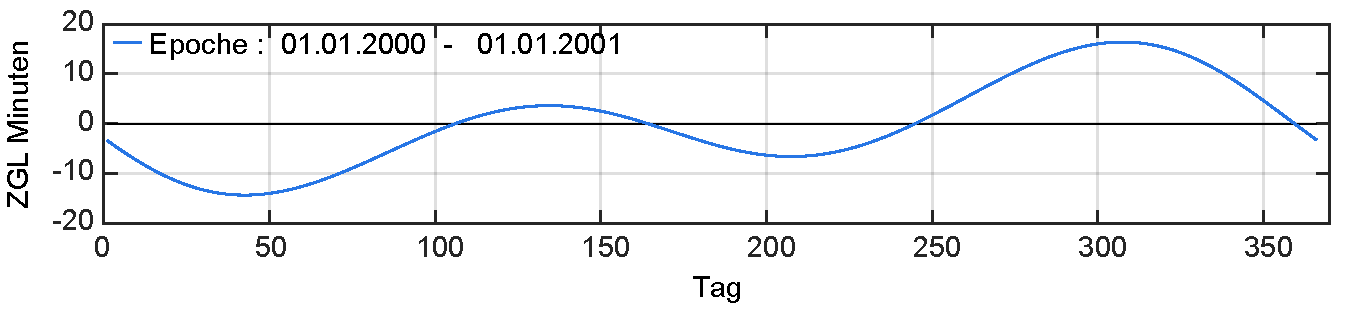
\includegraphics[width=\textwidth]{ZGL01a.pdf}\\
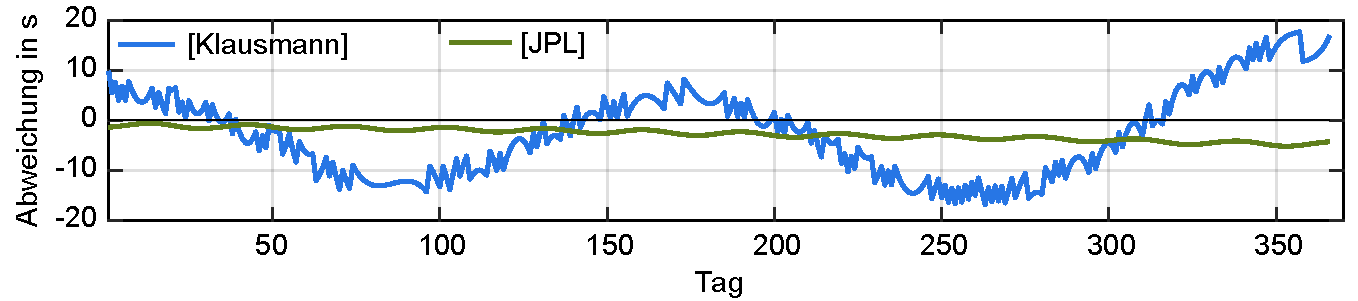
\includegraphics[width=\textwidth]{ZGL01b.pdf}\\
\caption[Berechnete Zeitgleichung und Abweichung von publizierten Werten.]{Berechnete Zeitgleichung und Abweichung von publizierten Werten nach Klausmann \cite{Klausmann1990} und JPL \cite{JPL2020}.}
\label{abb:hm_Zeitgleichung}
\end{figure}
Mit der Zeitgleichung \eqref{eq:hm_tau_zgl}, die in \figref{hm_Zeitgleichung} aufgetragen ist, k�nnen wir somit direkt die t�gliche Abweichung der Kulminationszeit der (wahren) Sonne von 12:00 lokaler (mittlerer) Ortszeit berechnen.
Wir erkennen, dass von Jahresbeginn bis ins Fr�hjahr die wahre Sonne der mittleren Sonne voraus ist.
Die Verh�ltnisse kehren sich dann im Sommer um.
Im Herbst und fr�hen Winter hinkt die wahre Sonne dann der mittleren hinterher. \\
Mit \eqref{eq:hm_UT_3} l�sst sich die Kulminationszeit f�r jede geographische L�nge einfach berechnen.
\figref{hm_Zeitgleichung} zeigt die Abweichung unserer Rechnung von hochgenauen Rechnungen wie sie vom JPL \cite{JPL2020} zur Verf�gung gestellt werden.
Die �bereinstimmung ist sehr gut.%
\footnote{In der Abbildung wird sichtbar, dass in der JPL-Rechnung St�rungen der reinen Keplerbahn durch den Mond zu einer periodischen Abweichung in Monatsabst�nden und zu einer Abweichung auf einer gr��eren Zeitskala f�hren.}
Beim Vergleich mit den empirischen Daten aus \cite{Klausmann1990} muss man ber�cksichtigen, dass diese �ber viele Jahre gemittelt wurden, sodass hier neben dem Schaltjahreseffekt\index{Schaltjahr} (366 anstelle von 365 Tagen) auch j�hrliche Ver�nderungen der Bahnparameter und insbesondere des Fr�hlingspunktes eingehen.

Tr�gt man f�r die Sonne deren Deklination �ber ihren Stundenwinkel (f�r \zb 12:00 UT) f�r jeden Tag des Jahres auf, dann erh�lt man ein sogenanntes \emph{Analemma}\index{Analemma}\glslink{analemma}.
In \figref{hm_Analemma_01} zeigen wir Analemmas f�r jeweils drei verschiedene Exzentrizit�ten $e$ und Ekliptikschiefen $\epsilon$.
W�re die Erdbahn kreisf�rmig und die Erdachse normal zur Ekliptik, dann w�re die Zeitgleichung konstant gleich $0$.
Die Abh�ngigkeit des Analemmas von Exzentrizit�t $e$ und Ekliptikschiefe $\epsilon$ kann man zur Bestimmung dieser Parameter aus dem Analemma nutzen (\mscr e \mlhmref{AnalemmaOkoFit.m} und \mlhmref{AnalemmaFindExz.m}). 

\begin{figure}
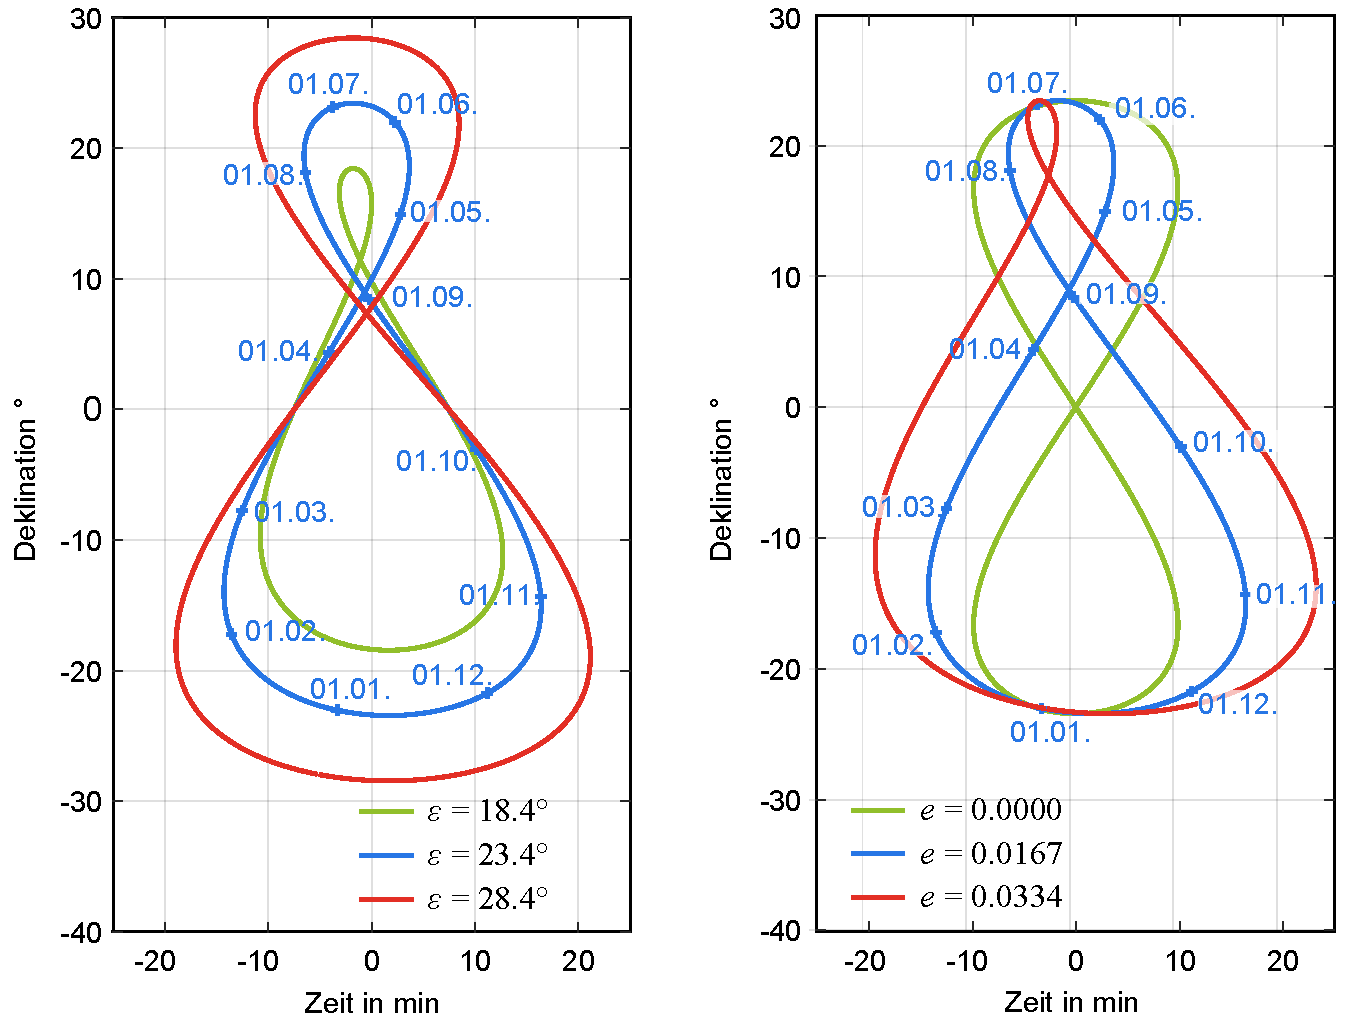
\includegraphics[width=\textwidth]{Analemma01.pdf}
\caption[Berechnete Analemmas f�r verschiedene Parameter.]{Berechnete Analemmas f�r verschiedene Parameter $\epsilon$, $e$ (vgl. \mscr{} \mlhmref{Analemma01.m}).}
\label{abb:hm_Analemma_01}
\end{figure}

Zur Beobachtung eines Analemmas nimmt man im Laufe eines Jahres an jedem Tag zum gleichen Zeitpunkt (auf $\pm 2\:\text{s}$ genau) mit einer fest montierten Kamera (Sonnenbeobachtungs-Schutzfilter nicht vergessen!) ein Bild auf und �berlagert am Ende eines Jahres alle Aufnahmen mit einem Hintergrundbild.%
In \figref{hm_Analemma_02} zeigen wir ein Analemma, welches in den Jahren 2019/20 t�glich um 08:40 MOZ aufgenommen wurde und dessen Fit an die berechnete Kurve (\mscr{} \mlhmref{AnalemmaOkoFit.m}).\footnote{Das Komposit wurde von Bertram H�nlinger, Dietmar Mondon und Michael Kaschke mit einer Nikon D800 und einem ZEISS Classic Distagon T$\ast$ 2.8/21 ZF.2 Objektiv aufgenommen. Man bekommt so �brigens auch einen nachtr�glichen Wetterbericht �ber die Anzahl der Sonnentage.} 
Um einen Fit mit den berechneten Kurven zu bekommen, �berf�hrt man sowohl die Aufnahmedaten als auch die Vorw�rtsberechnungen in das topozentrisch-horizontale KOS, wobei es dabei zu den charakteristischen Verzeichnungen kommt.
Man erkennt sehr gut, dass die Annahme einer doppelt so gro�en Exzentrizit�t der Erdbahn zu einer massiven Abweichung des berechneten Analemmas von der beobachten Kurve f�hren w�rde.
F�r die Bilddatenumrechnung sei an dieser Stelle auf die detaillierte Darstellung in \cite{Montenbruck2001} und \cite{Smart1986} verwiesen. 

\begin{figure}
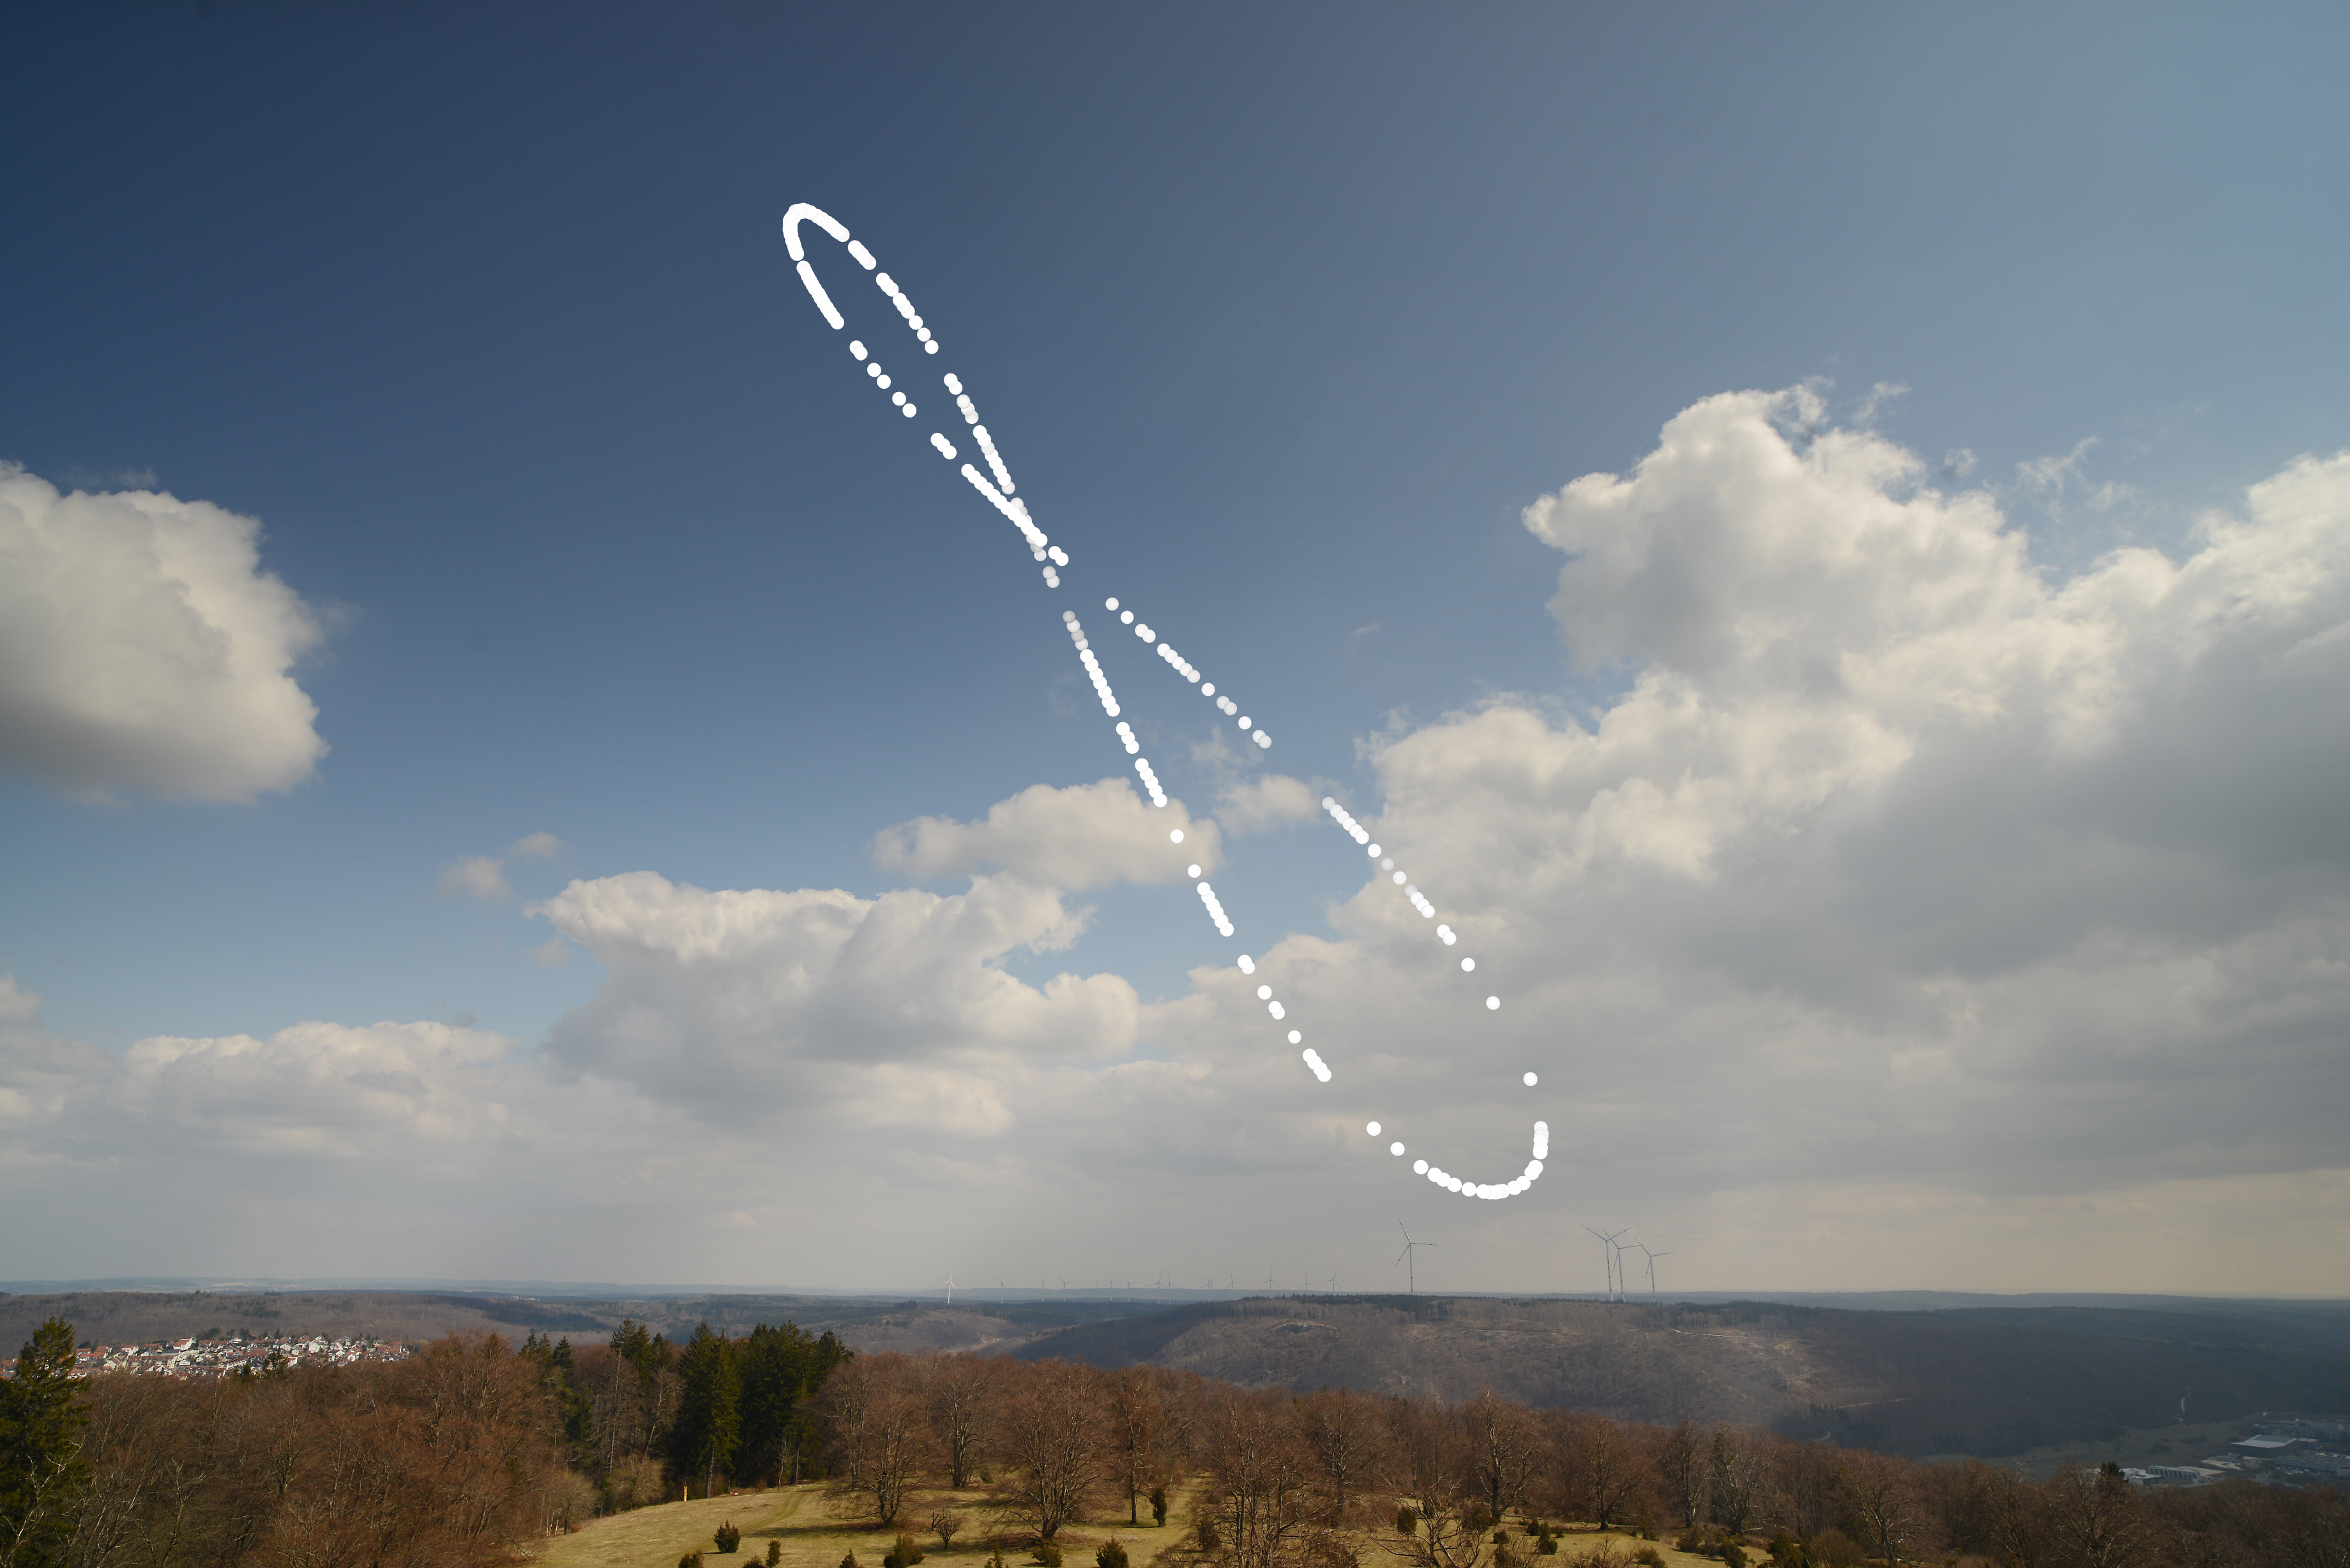
\includegraphics[width=1.0\textwidth]{Analemma2020.jpg}
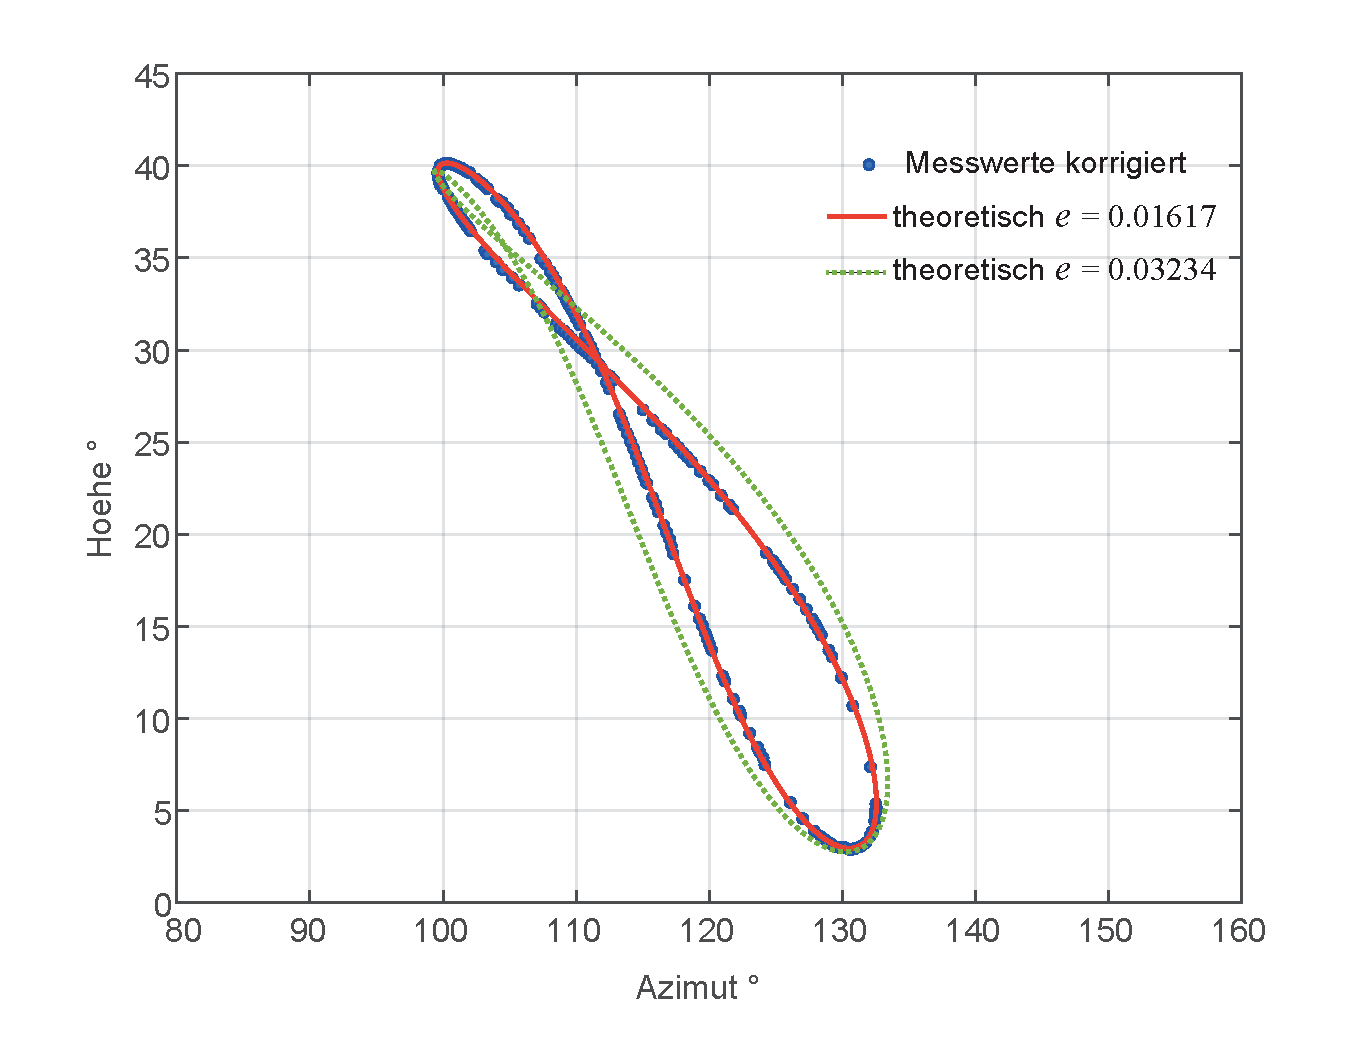
\includegraphics[width=1.0\textwidth]{Analemmafit.pdf}
\caption[Aufnahme eines Analemmas in den Jahren 2019/2020.]{Aufnahme eines Analemmas in den Jahren 2019/2020  und Fit mit der Exzentrizit�t als Parameter (Modellierung ausgef�hrt in den \mscr en \mlhmref{AnalemmaOkoFit.m} und \mlhmref{AnalemmaFindExz.m}).}
\label{abb:hm_Analemma_02}
\end{figure}

In \figref{hm_Analemma_03} haben wir noch schlie�lich berechnete Analemmas f�r zwei Standorte auf der Erde f�r verschiedene Tageszeiten dargestellt.
Man beachte die Effekte des Polarsommers \bzw Polarwinters auf das Analemma von Troms�.

\begin{figure}
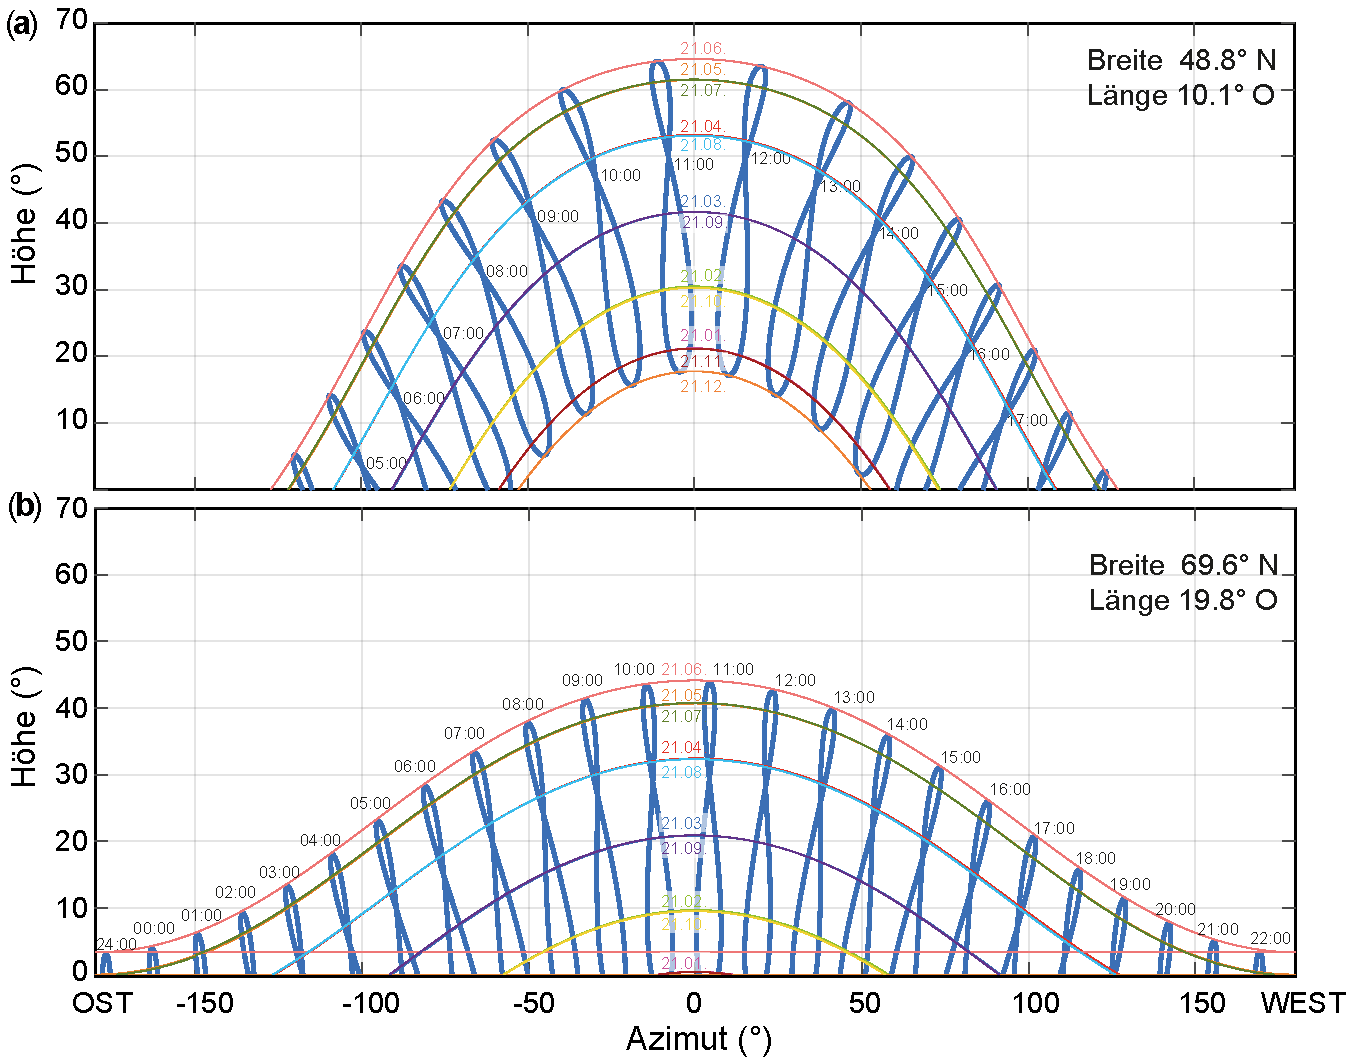
\includegraphics[width=1.0\textwidth]{Analemma03.pdf}
\caption[Berechnete Analemma-Bilder f�r zwei geographische Orte.]{Berechnete Analemma-Bilder f�r Oberkochen, Deutschland \fa und Troms�, Norwegen \fb \mscr{} (\mlhmref{Analemma02.m}).}
\label{abb:hm_Analemma_03}
\end{figure}

\subsubsection{Refraktionskorrekturen, Parallaxe}\index{Refraktionskorrektur}

Zur Berechnung von Auf- und Untergangszeiten\index{Aufgangszeiten}\index{Untergangszeiten} m�ssen wir das topozentrisch-horizontale KOS benutzen und den Stundenwinkel $\tau$ des Himmelsk�rpers bei $h\!=\!0$ mit \eqref{eq:hm_Alt-Az-Koord} berechnen.
Dabei m�ssen wir aber Einflussfaktoren wie Refraktion, Parallaxe und scheinbaren Durchmesser $D_\text{O}$ des Himmelsk�rpers ber�cksichtigen, die wir hier kurz vorstellen wollen. 

\subparagraph{\textbf{\gls{refraktion}}}
In der Astronomie ist vor allem die Ablenkung der Lichtstrahlen durch die Erdatmosph�re und die damit verbundene \anf{scheinbare} �nderung der Koordinaten von Bedeutung.
Physikalisch gesehen wird diese Brechung (Refraktion) der aus dem All kommenden Lichtstrahlen durch die optisch dichter werdenden Schichten der Atmosph�re verursacht.
Als Folge davon werden die Lichtstrahlen zur Erde hin gekr�mmt (\probref{hm_refrak_optik}).
Da Beobachter immer von einer geradlinigen Ausbreitung ausgehen, weicht die Beobachtungsrichtung vom tats�chlichen Lichtweg ab (\figref{hm_refraktion}).
Alle Objekte werden daher unter einer gr��eren H�he (der scheinbaren H�he $h'$) als der wahren, d.\,h. berechneten (sogenannten astrometrischen) H�he\index{H�he!wahre}\index{H�he!scheinbare}\index{H�he!astrometrische} $h$ gesehen.
Der Unterschied ist in Horizontn�he am gr��ten und bei der Beobachtung eines Objektes im Zenit gleich Null. 

\begin{figure}
\begin{minipage}{\textwidth}
\leftfigure{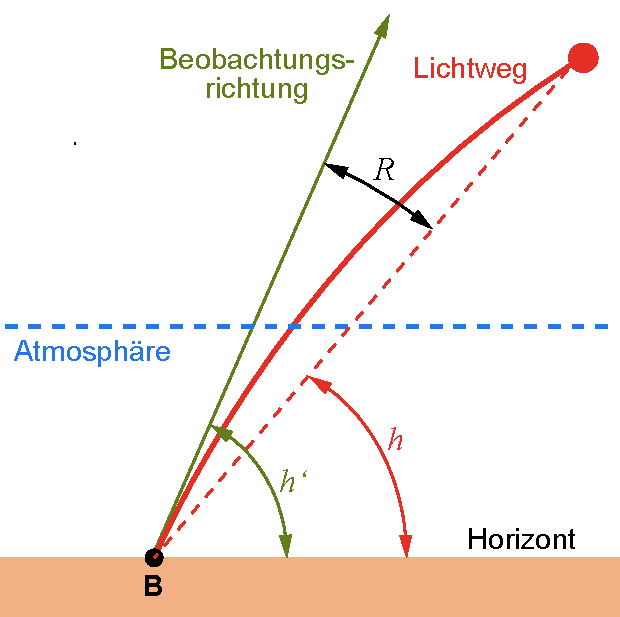
\includegraphics[width=0.5\textwidth]{Refraktion.pdf}}
\hspace{\fill}
\rightfigure{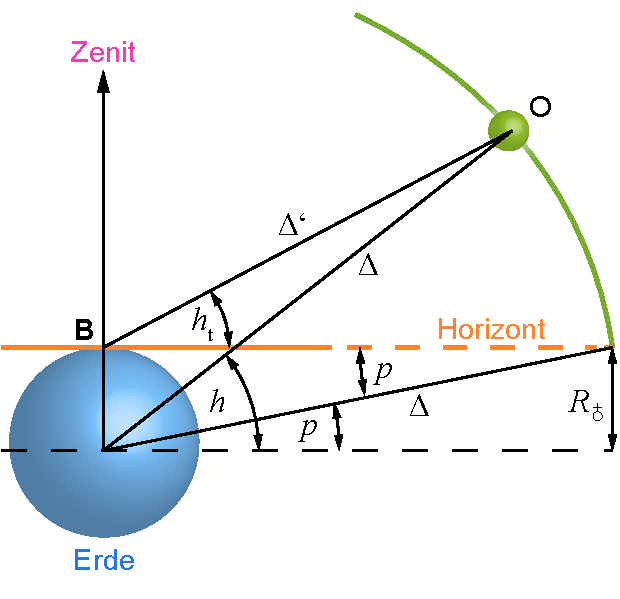
\includegraphics[width=0.5\textwidth]{TopozentrischeParallaxe.pdf}}
\leftcaption{Refraktion in der Himmelsbeobachtung.}\label{abb:hm_refraktion}
\rightcaption{Parallaxe und Horizontalparallaxe.}\label{abb:hm_parallaxe}
\end{minipage}
\end{figure}

Die sogenannte \emph{Refraktionskurve}\index{Refraktionskurve} $R(h')\!=\!R(90\degree-z')=h'-h$ gibt die Abh�ngigkeit von der scheinbaren H�he\index{H�he!scheinbare} $h'$ �ber dem Horizont bzw. von der Zenitdistanz $z'\!=\!90\degree-h'$ an.\footnote{Ungl�cklicherweise bezeichnet man die Refraktion mit $R$, was oft zu Verwechslungen mit Radien und Abmessungen f�hrt. Da in der Literatur und insbesondere in Tabellen aber $R$ benutzt wird, halten wir uns ebenfalls an die Konvention.}
Der genaue Wert h�ngt von vielen Parametern ab, \ua den Brechzahlen der Luftschichten, die wiederum eine Funktion der atmosph�rischen Bedingungen wie Druck, Temperatur und der geographischen Breite sind.
Zur Berechnung von $R(h')$ ausgehend von der scheinbaren H�he (oder alternativ $R(h)$), wurden verschiedene Modelle entwickelt (\probref{hm_refrak_optik}), woraus entsprechende Refraktionstafeln berechnet wurden.
F�r unsere Zwecke reicht zun�chst die Betrachtung der sogenannten Normalrefraktion in Horizontn�he.
Man kann dabei mit folgenden Formeln arbeiten \cite{Meeus1998}, wobei $h$ bzw. $h'$ in \textdegree\ einzusetzen sind und das Ergebnis in Bogenminuten ausgegeben wird:
\begin{equation} \label{eq:hm_Normalrefraktion1}
R(h')=h'-h=\frac{1}{\tan \lk{h'+\frac{7.31\degree}{h'+4.4\degree}}\rk} ~~~\left[ \text{Ausgabe in Bogenminuten} \right] ~,
\end{equation}
\begin{equation} \label{eq:hm_Normalrefraktion2}
R(h)=h'-h=\frac{1}{\tan\lk{h+\frac{10.3\degree}{h+5.11\degree}}\rk} ~~~ \left[ \text{Ausgabe in Bogenminumten} \right] ~.
\end{equation}

F�r die Bestimmung eines Aufgangs ist die scheinbare H�he gleich Null.
Man muss also den Zeitpunkt f�r $h\!=\!-R(h'\!=\!0)$ berechnen.
Aus \eqref{eq:hm_Normalrefraktion1} bestimmt man $R(h'\!=\!0)\!=\!34'$.
Mit diesem Wert werden wir nun weiterrechnen.

\subparagraph{\textbf{\gls{parallaxe}}}\index{Parallaxe}
Wir hatten bereits in \kapitel{hm_koordinatensysteme} auf den Unterschied zwischen einem topozentrischen und einem geozentrischen KOS hingewiesen und in Tabelle \ref{tab:hm_Umrechung_KOS} auch die Transformation zwischen beiden angegeben.
Der Unterschied zwischen beiden KOS muss dann ber�cksichtigt werden, wenn der Erdradius im Verh�ltnis zum Abstand des beobachteten Himmelsobjektes nicht mehr zu vernachl�ssigen ist.
Das ist auf alle F�lle beim Mond im Verh�ltnis zur Erde, aber auch den inneren Planeten und unter Umst�nden (\zb bei Berechnung von Sonnenfinsternissen) bei der Sonne der Fall.
Durch die Parallaxe ist die topozentrische H�he $h_\text{t}$ kleiner als die geozentrisch (berechnete) H�he $h_\text{g}$.
Die Parallaxe wirkt also der Refraktion entgegen.
Wir k�nnen f�r $h_\text{t}\!=\!0$ die sogenannte Horizontalparallaxe aus \figref{hm_parallaxe} bestimmen zu
\begin{equation} \label{eq:hm_Parallaxe}
p=\arcsin\lk \frac{R_\text{\earth}}{\Delta} \rk ~.
\end{equation}
F�r die Sonne berechnet sich ein Betrag von etwa 9'' (Bogensekunden), f�r den Mond schon betr�chtliche 57' (Bogenminuten).
Die Parallaxe ist also beim Mond definitiv nicht mehr zu vernachl�ssigen.


\subparagraph{\textbf{Scheinbarer Durchmesser}}\index{Durchmesser!scheinbarer|textbf} 
F�r die Aufgangsberechnung haben wir au�erdem noch den Winkeldurchmesser $D_\text{O}$ des Himmelsobjektes zu ber�cksichtigen, unter dem dieses von der Erde aus erscheint.
Wir messen bei Aufg�ngen das Erscheinen des oberen Rands, m�ssen also $R_\text{O}\!=\!D_\text{O}/2$ in der Berechnung der Aufgangsh�he ber�cksichtigen.
Mit $D_\text{O \astrosun} = 32'$ und $D_\text{O M} = 29' \ldots 34'$ ergibt sich insgesamt f�r die Korrektur der H�he
\begin{equation}\label{eq:hm_Parallaxe_2}
h_\text{A,U}=0\text{\textdegree}-R\lk h'=0 \rk +p-R_\text{O} =  \begin{cases} -50' ~~ &\text{Sonne} \\ +\; 6' \ldots 8' ~~ &\text{Mond}\end{cases}  ~.
\end{equation}


\subsubsection{Berechnung der Auf- und Unterg�nge} \label{kap:auf-untergaenge}\index{Aufg�nge}\index{Unterg�nge}
Wir k�nnten nun $h_\text{A,U}$ aus \eqref{eq:hm_Parallaxe_2} in \eqref{eq:hm_Alt-Az-Koord} einsetzen und den Stundenwinkel $\tau$ bzw. die Sternzeit $\theta$ bestimmen, woraus sich wiederum die Ortszeit f�r den Auf- \bzw Untergang bestimmen l�sst.
Da aber bei der Sonne sowohl Rektaszension $\alpha$ als auch Deklination $\delta$ selbst zeitabh�ngig sind, k�nnen wir die transzendente Bestimmungsgleichung \eqref{eq:hm_Alt-Az-Koord} nicht analytisch, sondern nur mittels numerischer Verfahren l�sen.
Dazu geht man iterativ vor:
\begin{enumerate}
	\item Man startet mit der Berechnung der \gls{sternzeit} $\theta_i$ f�r $t_i\!=$ 12:00 UT aus dem Datum und der geographischen L�nge.
          Man berechnet daraus die Deklination $\delta_i$ und die Rektaszension $\alpha_i$, die die Sonne zu dieser Zeit hat.
          Daraus ergibt sich der Stundenwinkel $\tau_i\!=\!\theta_i-\alpha_i$. 
	\item Wir berechnen dann den Stundenwinkel $T_i$ aus \eqref{eq:hm_Alt-Az-Koord} und daraus eine neue Uhrzeit $t_{i+1}$ f�r den Auf- bzw. Untergang mittels
\begin{align}
T_i &= \pm \lk \frac{1^\text{h}}{15\degree} \rk \arccos\lk \frac{\sin h_\text{A,U}-\sin\delta(\tau_i)\sin\varphi}{\cos\delta(\tau_i)\cos\varphi}\rk \label{eq:hm_std_winkel_Ti} ~,\\
t_{i+1} &=t_i + (T_i-\tau_i) ~.\nonumber
\end{align}
Dabei muss man auf einige Sonderf�lle achten, z.\,B. wenn $T_i$ in \eqref{eq:hm_std_winkel_Ti} komplex wird.
Dann geht die Sonne an dem Tag nicht unter, was z.\,B. im Polarsommer in hohen geographischen Breiten der Fall sein kann. 
\end{enumerate}
Eine alternative Methode der Berechnung besteht darin, dass man f�r den Tag von 0:00 bis 24:00 in Intervallen von z.\,B. 1 h die H�he $h_\text{A,U}$ als Funktion der Ortszeit (bzw. Sternzeit) berechnet und in den Intervallen nach m�glichen Nullstellen sucht.
Dazu eignen sich numerische Nullstellenverfahren.
Wir folgen in \mlhmref{Sonnenaufgang01.m} \bzw \mlhmref{Sonnenaufgang02.m} diesem Weg (siehe auch \cite{Montenbruck1999}) und nutzen die Methode der quadratischen Interpolation.
Diese bietet den Vorteil, gegebenenfalls auch zwei Nullstellen in einem Intervall ermitteln zu k�nnen.
Das Programm ist in dieser Form auch anwendbar auf die Berechnung von Auf- und Untergangszeiten des Mondes oder von Satelliten, sofern man die Berechnungsformeln f�r deren �quatoriale Koordinaten kennt. 

Das Ergebnis einer Sonnenauf- und -untergangs-Berechnung ist in \figref{hm_Sonnenauf_untergang} f�r Oberkochen ($\phi\!=\!48.8\degree$ und $\lambda\!=\!10.1\degree$) zu sehen.
Man erkennt in der vergr��erten Darstellung (rechtes Bild) sehr sch�n, dass der k�rzeste Tag des Jahres wegen der ZGL weder mit dem fr�hesten Sonnenuntergang noch auch mit dem sp�testen Sonnenaufgang zusammenf�llt.

\begin{figure}%
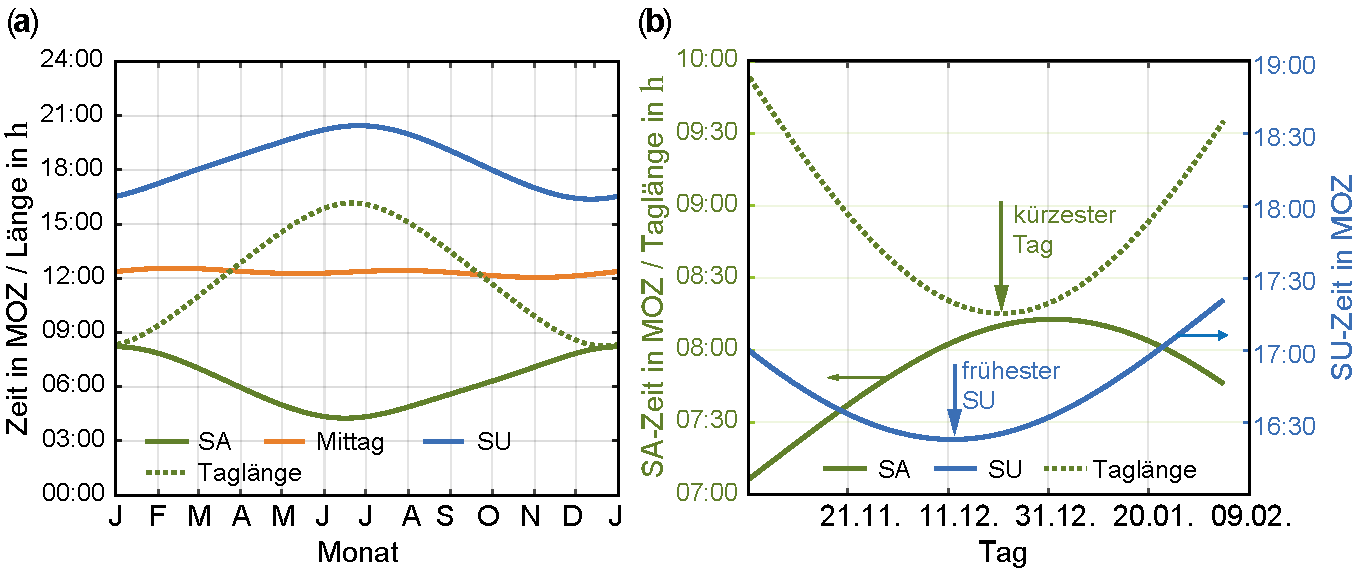
\includegraphics[width=\textwidth]{Sunrise01.pdf}\\%
\caption[Berechnung der Sonnenaufgangs- und Sonnenuntergangszeiten.]{Berechnung der Sonnenaufgangs- und Sonnenuntergangszeiten. \fa SA, SU, Tagl�nge in Oberkochen (Breite $\phi\!=\!48.8\degree$ und L�nge $\lambda\!=\!10.1\degree$). \fb SA, SU und Tagl�nge um den Jahreswechsel. Die $x$-Achse in \fa ist mit den Anfangsbuchstaben der Monate bezeichnet.}%}%
\label{abb:hm_Sonnenauf_untergang}%
\end{figure}

\subsubsection{N�herungsformeln und deren Herleitung} \label{kap:hm_naeherungsformeln_sonne}
\subparagraph{\textbf{Reihenentwicklung der Zeitgleichung}}
Wir wollen jetzt handhabbare Formeln f�r die Zeitgleichung sowie Auf- und Untergangszeiten der Sonne herleiten.
Dazu starten wir mit der geozentrischen Darstellung in \figref{hm_wahre_sonne_geoz}. 
\begin{figure}%
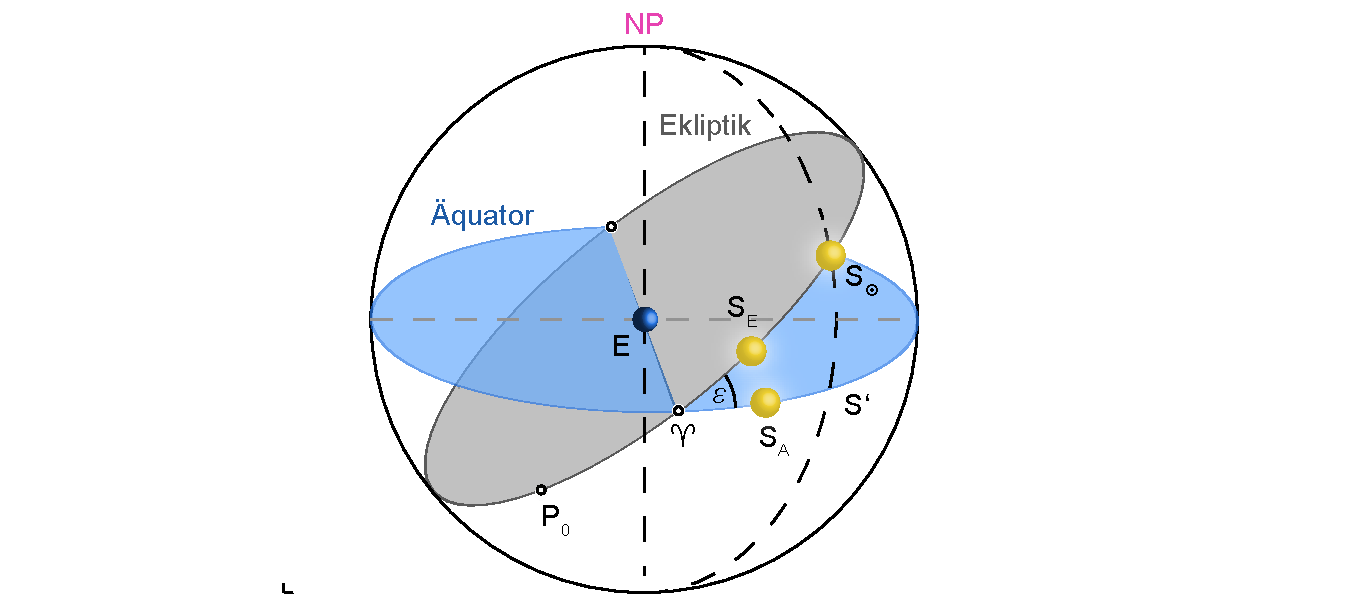
\includegraphics[width=\textwidth]{Wahre_und_mittlere_Sonne.pdf}%
\caption{Bewegung der wahren und der mittleren Sonne im geozentrischen Bild.}%
\label{abb:hm_wahre_sonne_geoz}%
\end{figure}
In dieser Abbildung haben wir neben der \anf{wahren} Sonne $\text{S}_\text{\astrosun}$ zwei weitere \anf{Hilfssonnen} $\text{S}_\text{E}$ und $\text{S}_\text{A}$ eingezeichnet.
Die Sonne $\text{S}_\text{A}$ bewege sich mit konstanter Umlaufgeschwindigkeit in der �quatorebene und die Sonne $\text{S}_\text{E}$ ebenfalls mit konstanter Winkelgeschwindigkeit auf der Ekliptik.
Die wahre Sonne $\text{S}_\text{\astrosun}$ bewege sich entlang der Ekliptik entsprechend der Keplergesetze mit ver�nderlicher Geschwindigkeit.
Die Hilfssonnen sind so definiert, dass beide mit der wahren Sonne in den �quinoktien\index{Aequinoktium@�quinoktium} \glslink{aequinox} zusammentreffen.
In \figref{hm_wahre_sonne_geoz} sind die geozentrischen Parameter entsprechend denen des heliozentrischen Bildes von \figref{hm_planetenbahnen_rel_ekliptik} definiert.
\begin{align*}
\lambda_\text{\astrosun}&=\angle\vernal\text{ES}_\text{\astrosun}       ~&\text{L�nge der wahren Sonne} \\
\Lambda_\text{M}&=\Lambda_\text{\astrosun}=\angle\vernal\text{ES}_\text{E}~&\text{L�nge der mittleren Sonne}  \\
\alpha_\text{\astrosun}&=\angle\vernal\text{ES'}          ~&\text{Rektaszension der wahren Sonne}  \\
\alpha_\text{M}&=\angle\vernal\text{ES}_\text{A}          ~&\text{Rektaszension der mittleren Sonne}  \\
\upsilon&=\lambda_\text{\astrosun}-\varpi=\angle\text{P}_0\text{ES}_\text{\astrosun}  ~&\text{wahre Anomalie}  \\
M&=\Lambda_\text{\astrosun}-\varpi=\angle\text{P}_0\text{ES}_\text{E}~&\text{mittlere Anomalie}
\end{align*}

Da die beiden Hilfssonnen mit gleicher Geschwindigkeit umlaufen, gilt $\Lambda_\text{\astrosun}\!=\!\alpha_\text{M}$.
Mit der Definition der Zeitgleichung \eqref{eq:hm_tau_zgl} erh�lt man
\begin{align}
\begin{split}  
\tau_\text{ZGL} &= \text{WOZ} - \MOZ = (\theta - \alpha_\text{\astrosun}) - \underbrace{(\theta-\alpha_\text{M})}_{0} = \alpha_\text{M}-\alpha_\text{\astrosun} = \Lambda_\text{\astrosun}-\alpha_\text{\astrosun} \\ 
&= (\Lambda_\text{\astrosun} - \lambda_\text{\astrosun}) + (\lambda_\text{\astrosun}-\alpha_\text{\astrosun}) = (\Lambda_\text{\astrosun} + \varpi) - (\lambda_\text{\astrosun}+\varpi)+(\lambda_\text{\astrosun}-\alpha_\text{\astrosun})  \\
&=\underbrace{(\Lambda_\text{\astrosun}-\varpi) - (\lambda_\text{\astrosun}-\varpi)}_{-\mathcal{C}\text{, siehe \eqref{eq:hm_mpglg_nu-M}}} + \underbrace{(\lambda_\text{\astrosun} -\alpha_\text{\astrosun})}_{\text{Reduktion $\mathcal{R}$, siehe \eqref{eq:hm_reduktions_formel4}}} \,. 
\end{split} \label{eq:hm_tau_ZGL_C}
\end{align}
Die ersten beiden Terme ergeben also den negativen Wert der Mittelpunktsgleichung.
Der dritte Term ist die sogenannte \emph{\gls{reduktion}}\index{Reduktion} der Ekliptik auf den �quator, \dh die Differenz zwischen bekannter ekliptikaler L�nge und gemessener �quatorialer Rektaszension.
Die Herleitung dieser Reduktion, die nur von $\lambda_\text{\astrosun}$ und $\epsilon$ abh�ngt, ist in \kapitel{reduktion_ekliptik} in Beispiel \ref{bsp:herleitung_redformel_ekl} detailliert ausgef�hrt. 
Wir benutzen hier das Ergebnis der Rechnung und erhalten 
\begin{align}
\begin{split}
\tau_\text{ZGL} &= -C+(\lambda_\text{\astrosun}-\alpha_\text{\astrosun}) \\
                &= -C+\tan^2\lk\frac{\epsilon}{2}\rk \sin(2\lambda_\text{\astrosun})-\frac{1}{2}\tan^4 \lk \frac{\epsilon}{2}\rk \sin(4\lambda_\text{\astrosun})+\mathcal{O}\lk \tan^6 \lk \frac{\epsilon}{2} \rk\rk \,. 
\end{split} \label{eq:hm_tau_ZGL_C1}
\end{align}
Man kann sich also merken: Die \emph{Zeitgleichung} ist die Summe von (negativer) Mittelpunktsgleichung (\emph{Wirkung der Exzentrizit�t}) und Reduktion der Ekliptik\index{Reduktion!auf den �quator} auf den �quator (\emph{Wirkung der Ekliptikschiefe}).
Wir wollen jetzt in der Form der ZGL \eqref{eq:hm_tau_ZGL_C1} die i.\,A. nicht bekannte ekliptikale L�nge der wahren Sonne $\lambda_\text{\astrosun}$ durch die tabellierte bzw. die einfach berechenbare L�nge $\Lambda_\text{\astrosun}$ der mittleren Sonne ersetzen.
Wir k�nnen dabei folgende Beziehungen nutzen:
\begin{align*}
\lambda_\text{\astrosun} &= \Lambda_\text{\astrosun} + \mathcal{C} =\Lambda_\text{\astrosun}+2e\sin M + \frac{5}{4}e^2\sin(2M) +\mathcal{O}(e^3) \,,\\
\sin(2\lambda_\text{\astrosun}) &\approx \sin(2\Lambda_\text{\astrosun})+4e\sin M \cos(2\Lambda_\text{\astrosun}) +\mathcal{O}(e^3)\,,\\
\sin(4\lambda_\text{\astrosun}) &\approx \sin(4\Lambda_\text{\astrosun}) + \mathcal{O}(e^3)\,.
\end{align*}
Mit der Abk�rzung $y=\lek\tan\lk\frac{\epsilon}{2}\rk\rek^2$ erhalten wir dann
 \begin{align*}
\tau_\text{ZGL} &= -\mathcal{C} + \underbrace{y \sin(2\Lambda_\text{\astrosun})- \frac{1}{2} y^2 \sin(4\Lambda_\text{\astrosun})}_{\text{T}_\text{I}} + 
\underbrace{4 e y \cos(2\Lambda_\text{\astrosun}) \sin(M)}_{\text{T}_\text{II}}  ~.\label{eq:hm_tau_ZGL_D}
\end{align*}
Der Term $\mathcal{C}$ beschreibt wie bereits erw�hnt den Effekt der Exzentrizit�t, der Term $T_\text{I}$ den der Schiefe der Ekliptik; er verschwindet mit $\epsilon \rightarrow 0$.
Term  $T_\text{II}$ ist ein Mischterm.
$\Lambda_\text{\astrosun}$ ist in einschl�gigen Tabellen (siehe auch Tabelle \ref{tab:hm_bahnparameter} im Anhang) aufgef�hrt.
Wir ersetzen $M = \Lambda_\text{\astrosun} - \varpi$ und erhalten mit 
\begin{equation*}
\Lambda_\text{\astrosun} = n(t-t_0) + \Lambda_\text{\astrosun 0} = 359999.0498\degree \:t + 280.4656\degree ~~
\end{equation*}
und den bekannten Beziehungen f�r trigonometrische Funktionen die Zeitgleichung in der folgenden Form:
\begin{align}
\tau_\text{ZGL} &= \sum_{k} \alpha_k \sin(k\Lambda_\text{\astrosun}) + \beta_k\cos(k\Lambda_\text{\astrosun}) = \sum_{k} \gamma_k\sin(\kappa_k t+\delta_k)\,, \label{eq:hm_parameter_alpha_beta} 
\end{align}
wobei
\begin{align*}
\kappa_k &= kn\,\frac{2\pi}{360\cdot 36525}~, \:\gamma_k = -\frac{24\cdot 60}{2\pi}\sqrt{\alpha_k^2+\beta_k^2}~~\: \text{und} \\
\delta_k &= k \, \Lambda_{\astrosun,0}+\arctan\lk \frac{\beta_k}{\alpha_k}\rk -\pi ~.
\end{align*}
Die Koeffizienten der Summen $\alpha_k$, $\beta_k$ bzw. $y_k$, $\delta_k$, $\kappa_k$ sind Funktionen der Bahnparameter der Erde $e$, $\varpi$, $n$, $\Lambda_\text{\astrosun,0}$, sowie der Ekliptikschiefe $\epsilon$ und damit auch abh�ngig von der Zeit.\footnote{Wir kommen darauf in \kapitel{hm_langezeiten} zur�ck.
Man beachte, dass in \eqref{eq:hm_parameter_alpha_beta} nur die Entwicklung bis zur Ordnung $e^2$ enthalten ist.} Wir rechnen mit den Werten f�r das �quinoktium des Datums, $t$ sind wiederum die seit J2000 vergangenen Jahrhunderte.
Die Koeffizienten $y_k$ sind in Zeitsekunden umgerechnet und f�r die Sinus-Funktion nutzen wir $\sin(x-\pi)\!=\!-\sin x$.
F�r die Parameter $\alpha_k$, $\beta_k$ bis $k\!=\!4$ erhalten wir
\begin{align}
\begin{split}
\alpha_1 &= -2e\cos\varpi -2e\tan^2\lk\frac{\epsilon}{2}\rk\cos\varpi \,, ~~~\beta_1 = +2e\sin\varpi-2e\tan^2\lk\frac{\epsilon}{2}\rk\sin\varpi \,,   \\ 
\alpha_2 &= -\frac{5}{4}e^2\cos(2\varpi) +\tan^2\lk\frac{\epsilon}{2}\rk \,, ~~~\beta_2 = +\frac{5}{4}e^2\sin(2\varpi)\,,  \\
\alpha_3 &= +2e\tan^2\lk\frac{\epsilon}{2}\rk\cos\varpi \,, ~~~\beta_3 = -2e \tan^2\lk\frac{\epsilon}{2}\rk\sin \varpi \,, \\
\alpha_4 &= -\frac{1}{2}\tan^4\lk\frac{\epsilon}{2}\rk \,,  ~~~\beta_4 = 0 \,. 
\end{split}\label{eq:hm_parameter_alpha_beta2}
\end{align}
Daraus berechnen wir mit den Bahnparametern aus Tabelle \ref{tab:hm_bahnparameter} die Zeitgleichung in der �blichen Form: 
\begin{align}
\tau_\text{ZGL} &=\! 7.364186\,\sin(0.017202\, t_\text{d}-0.062882) \nonumber  \\
								& \!-9.93481\,\sin(0.034404\, t_\text{d} + 0.368790) + \ldots \label{eq:hm_ZGL21}
\end{align}
mit
\begin{align*}
y_k      &= \! (-7.364186,\,-9.93481,\,-0.329614,\,-0.21222, \ldots) ~~\text{in Zeitminuten,} \\
\kappa_k &= \! (0.017202,\,0.034404,\,0.051606,\,0.068808, \ldots) ~~\text{im Bogenma�,} \\
\delta_k &= \! (-0.062882,\,0.361758,\,0.321940,\,0.730548,\ldots) ~~\text{im Bogenma�}. 
\end{align*}
Hierin haben wir die Parameter $\kappa_k  \rightarrow 100 \kappa_k$ und $t\!\rightarrow \!t_\text{d}$ mit $t_\text{d} = 0 \ldots 365$ f�r die Tage eines Jahres gesetzt, was wegen der Periodizit�t in $\kappa_k$ f�r das Jahr 2000 streng gilt, f�r Jahre um 2000 n�herungsweise.\footnote{F�r andere Jahre muss man die Parameter \eqref{eq:hm_parameter_alpha_beta2} neu berechnen, siehe auch \kapitel{hm_altertum_zeiten}.} Dies ist die allgemein bekannte und gut handhabbare Form der Zeitgleichung.
Die ersten beiden Terme zeigen �ber \eqref{eq:hm_parameter_alpha_beta2} die Beitr�ge der Exzentrizit�t und der Ekliptikschiefe (\figref{hm_reihenent_zeitglg}).
Zur Verdeutlichung sind die deutlich kleineren Terme mit $3\omega$ und $4\omega$ jeweils um einen Faktor 10 vergr��ert dargestellt.
Da wir in unserer Berechnung wiederum sechs Bahnparameter (inklusive der Zeit $T_0$) benutzt haben, muss man die Reihe mindestens bis $k\!=\!2$ entwickeln, was meist schon ausreichend genaue Ergebnisse liefert.
Alle in der Literatur vorhandenen und leicht unterschiedlichen Zeitgleichungen basieren letztendlich auf dieser Grundform.
Sie unterscheiden sich in der Wahl des �quinoktiums und der Ordnung $k$ der Reihenentwicklung.
In \mlhmref{ZGL03.m} sind die verschiedenen publizierten Zeitgleichungen \cite{Wetzel2007,Rempel2019} miteinander verglichen.
\begin{figure}%
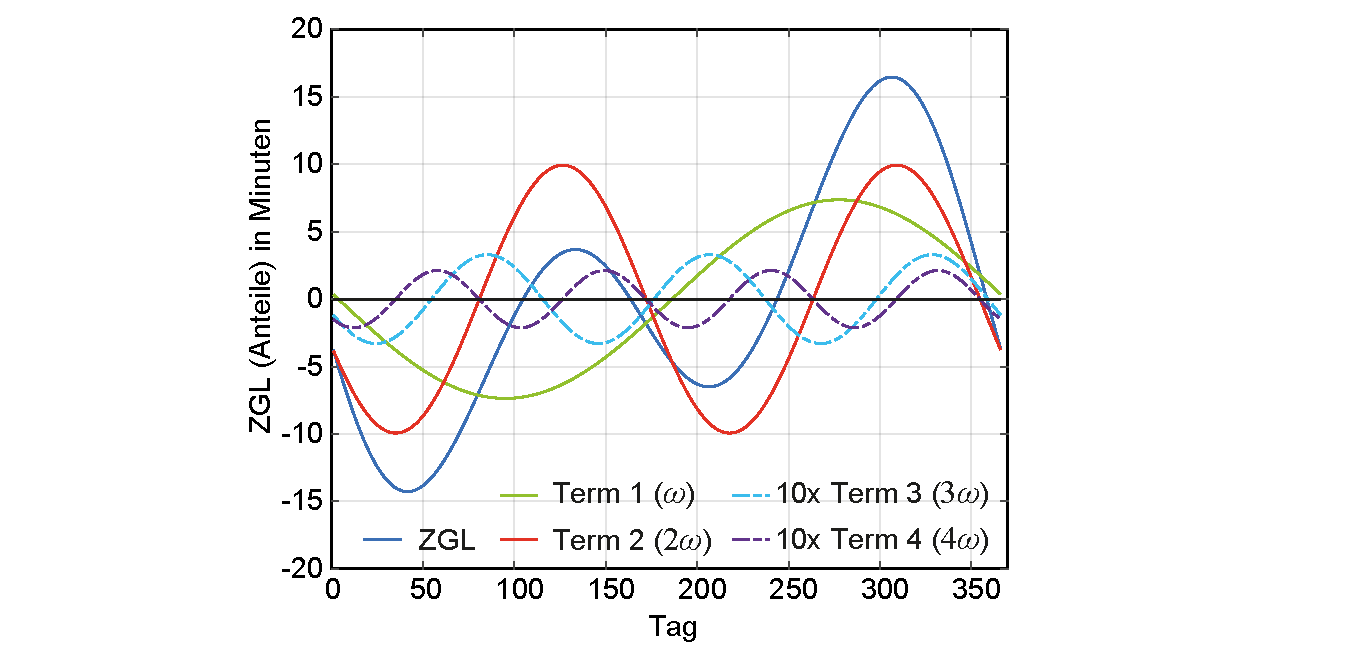
\includegraphics[width=\textwidth]{ZGL02.pdf}%
\caption{Reihenentwicklung der Zeitgleichung.}%
\label{abb:hm_reihenent_zeitglg}%
\end{figure}

Nach gleicher Methodik kann auch die Deklination als Funktion der seit einem Zeitpunkt vergangenen Tage $t_\text{d}$ berechnet werden.
Wir geben hier nur das erste Glied der Reihenentwicklung im Bogenma� an:
\begin{equation}
\delta(t_\text{d}) = 0.4095 \, \sin(0.016906 t_\text{d} - 1.35393) \,. \label{eq:hm_delta_von_T_hash}
\end{equation}

\subparagraph{{N�herungsformel f�r den Sonnenaufgang und Sonnenuntergang}}\index{Sonnenaufgang}\index{Sonnenuntergang}
Mit den beiden letzten Formeln wollen wir nun ebenfalls Berechnungsformeln f�r den Sonnenaufgang \bzw -untergang herleiten.
Wir haben in \kapitel{auf-untergaenge} zur Bestimmung des Aufgangs eines Himmelsk�rpers mit zeitlich ver�nderlicher Deklination und Rektaszension (wie z.\,B. Sonne und Mond) eine numerische Methode w�hlen m�ssen, weil es gem�� \eqref{eq:hm_Alt-Az-Koord} keine geschlossene Umkehrfunktion $\tau(h)$ zur Funktion $h(\tau)$  gibt.
Da sich aber die Deklination der Sonne im Verlauf eines Tages nur geringf�gig �ndert, lassen sich bei bekannter Zeitgleichung die Zeitpunkte f�r die Auf- und Unterg�nge der Sonne n�herungsweise mit relativ einfachen Formeln bestimmen, ohne dass man auf den mathematisch-numerischen Apparat f�r die iterative L�sung zur�ckgreifen muss.
Da der Kulminationszeitpunkt\glslink{kulmination}\ �ber die ZGL bekannt ist und die Deklination der Sonne innerhalb von $\pm 9$ h um den Kulminationszeitpunkt herum als n�herungsweise konstant angenommen werden kann, muss man nur noch den Schnittpunkt des Tagbogens der Sonne mit dem Horizont berechnen.
Als \emph{\gls{tagbogen}} wird der geometrische Bogen bezeichnet, den die Sonne (bzw. jeder andere Himmelsk�rper) �ber dem Horizont beschreibt.
\begin{figure}%
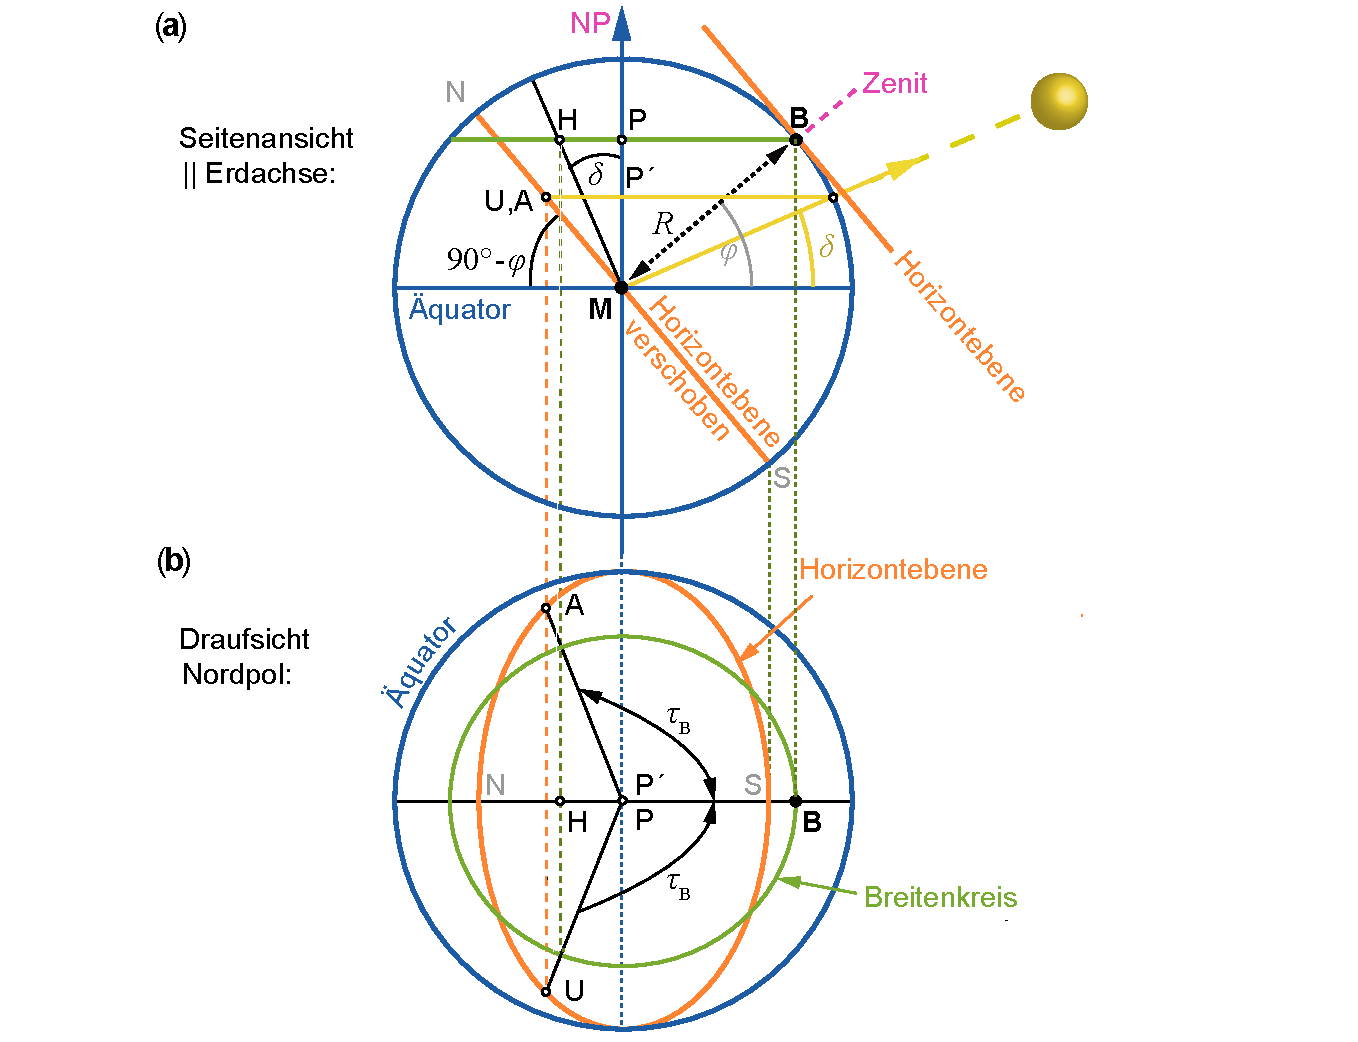
\includegraphics[width=\textwidth]{TagbogenGeometrie02.pdf}%
\caption[Geometrie des Tagbogens der Sonne.]{Geometrie des Tagbogens der Sonne (nach \cite{Praxl2016}) -- B Beobachter, A/U Auf- bzw. Untergangspunkt der Sonne am Horizont, N/S Nord-S�d-Richtung am Horizont. }%
\label{abb:hm_geom_tagbogen}%
\end{figure}
Wir betrachten dazu \figref{hm_geom_tagbogen} und k�nnen aus der Teilabbildung a direkt die folgenden Beziehungen ablesen:
\begin{align*}
\overline{\text{PM}} &= R \sin\varphi  = \overline{\text{PB}} \tan\varphi \,, \\
\overline{\text{PH}} &= \overline{\text{PM}} \tan\delta \,, \\
\rightarrow \frac{\overline{\text{PH}}}{\overline{\text{PB}}} &= \tan\varphi \tan\delta ~.
\end{align*}
Andererseits folgt aus der Teilabbildung b f�r den halben Tagbogen $\tau_\text{B}$ :
\begin{align}
\cos \tau_\text{B} \!&=\!-\cos(180\degree - \tau_\text{B}) = - \frac{\overline{\text{PH}}}{\overline{\text{PB}}} = -\tan\varphi\tan\delta ~~ \text{und somit} \nonumber \\
\tau_\text{B}\!&=\!\arccos(-\tan\varphi\tan\delta) ~.	\label{eq:hm_tau_B}
\end{align}
F�r die Aufgangszeiten erfolgt die Umrechnung von $\tau_\text{B}$ in Zeitstunden durch Multiplikation von $24 \text{h}/2\pi$.
Im Interesse �bersichtlicher Notation lassen wir die Umrechnungsfaktoren vom Bogenma� ins Zeitma� weg und gehen davon aus, dass $\tau_\text{B}$ genauso wie $\tau_\text{\,ZGL}$ in der jeweils f�r die Formel richtigen Einheit benutzt werden.
Bei der Benutzung von \eqref{eq:hm_tau_B} f�r die Aufgangszeiten\footnote{Die Formel \eqref{eq:hm_tau_B} gilt nur f�r $\abs{\tan\varphi\tan\delta}\!<\!1$, ansonsten wird der Himmelsk�rper zirkumpolar und geht weder auf noch unter, was im Sommer \zb in Breiten n�rdlich des Polarkreises f�r die Sonne der Fall ist.} m�ssen wir das Vorzeichen von $\tau_\text{B}$ beachten.
Zur Klarheit addieren oder subtrahieren wir $\abs{\tau_\text{B}}$ zur Kulminationszeit und erhalten dann f�r die Auf-/Untergangszeitpunkte 
\begin{equation}
t_\text{A,U} = \text{12:00 h} \,\text{UT} - \frac{\lambda}{15}+ \tau_\text{ZGL} + \tau_\text{A,U} ~~\text{mit}~~ \tau_\text{A} = -\abs{\tau_\text{B}} \text{ bzw. } \tau_\text{U} = \abs{\tau_\text{B}} \,. \label{eq:hm_untergangszeitp}
\end{equation}
Man ber�cksichtige, dass $\abs{\tau_\text{B}}$ in \eqref{eq:hm_untergangszeitp} von der Deklination $\delta$ nach \eqref{eq:hm_ZGL21} abh�ngt und somit ebenso wie $\tau_\text{ ZGL}$ vom jeweiligen Tag.
Jetzt m�ssen wir aber noch den Effekt der Refraktion und des scheinbaren Durchmessers der Sonne ber�cksichtigen.
Wir nehmen wieder die Refraktion in Horizonth�he mit $R\!=\!34'$ an, den scheinbaren Radius der Sonne mit $d_\text{\astrosun}/2=16'$ und vernachl�ssigen die Parallaxe.
In erster N�herung ist dann der beobachtete Tagbogen in Horizontn�he gegen�ber dem geometrisch-astronomischen (wahren) Tagbogen parallel verschoben (\figref{hm_verl_tagbogen_ref}), was zu einer Nordverschiebung des Azimuts beim Sonnenaufgang f�hrt.
Damit einher geht eine Tagbogenverl�ngerung\index{Tagbogenverl�ngerung} $\Delta\tau_\text{B}$, \dh die Sonne ist wegen der Refraktion fr�her am Himmel sichtbar als es rein geometrisch-astrometrisch der Fall w�re.
Die (halbe) Tagbogenverl�ngerung ist die Zeit, die die Sonne br�uchte, um die H�he $h_r\!=\!R+d_\text{\astrosun}/2$ zu durchlaufen.
Wir starten gem�� \eqref{eq:hm_Alt-Az-Koord} mit
\begin{equation*}
\sin h(t) = \cos\delta(t) \cos\tau \cos\varphi + \sin\delta(t)\sin\varphi ~~\text{und}~~0<t<24\:\text{h} \,.
\end{equation*}

\begin{figure}%
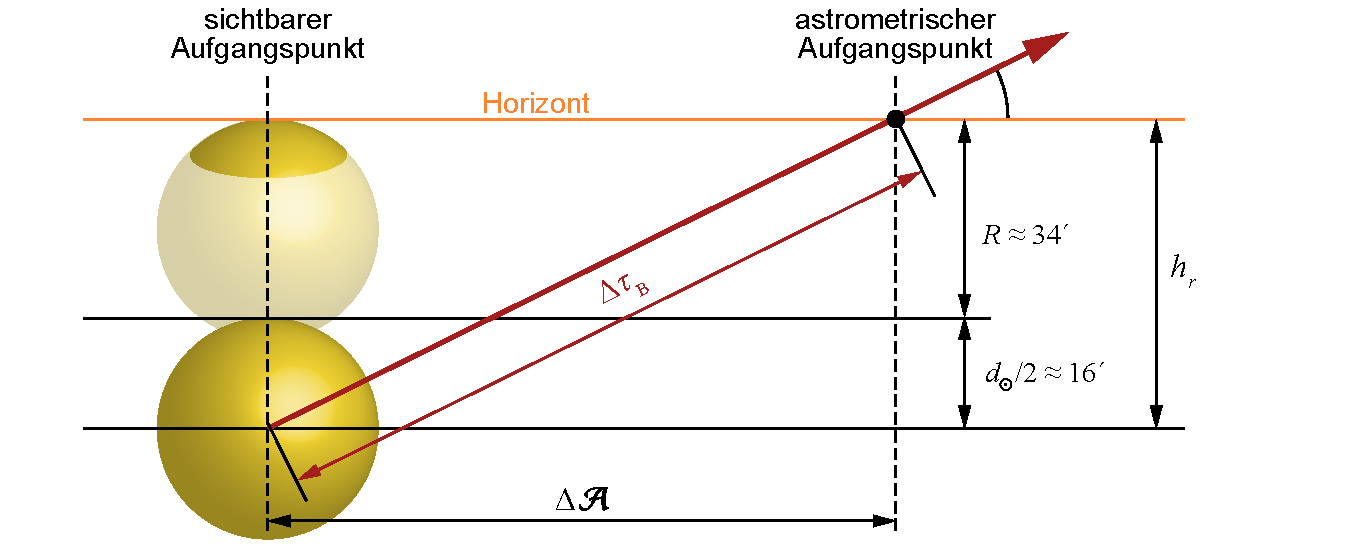
\includegraphics[width=\textwidth]{Tagbogenverlaengerung.pdf}%
\caption[Tagbogenverl�ngerung durch Refraktion und scheinbaren Durchmesser.]{Verl�ngerung des Tagbogens durch Refraktion und scheinbaren Durchmesser.}%
\label{abb:hm_verl_tagbogen_ref}%
\end{figure}

Ber�cksichtigen wir, dass $\D t=\D \tau$, wir ferner f�r die kleine Zeitspanne des Aufgangs die Deklination der Sonne $\cos\delta(t)\!=\!\cos\delta_\text{A}$ als konstant annehmen k�nnen und f�r sehr kleine H�hen $\sin h\!\approx\!h$ und $\cos h\!\approx\! 1$ gilt, k�nnen wir die Vertikalgeschwindigkeit der Sonne zum Stundenwinkel des Aufgangs wie folgt berechnen:
\begin{equation*}
\frac{\D h}{\D \tau} \bigg|_{\tau_\text{A}}\! = -\cos\delta\cos\varphi\sin\tau_\text{A} \,.
\end{equation*}
Man beachte hierbei die Winkel-Zeitumrechnung entsprechend $2\pi\!\hat{=}\!24 \:\text{h}$.
Die Tagbogenverl�ngerung (beim Aufgang) k�nnen wir dann zu
\begin{align}
\Delta\tau_\text{A} &= \frac{h_r}{\lk \frac{\D h}{\D \tau}\rk} = \frac{h_r}{-\cos\delta\cos\varphi\sin\tau_\text{A}} 
\nonumber \\
&= -\frac{h_r}{\cos\delta\cos\varphi\sqrt{1-\cos^2\tau_\text{A}}} = -\frac{h_r}{\sqrt{\cos^2\delta-\sin^2\varphi}} \,\label{eq:hm_tagbogverl}
\end{align}
ermitteln. Wie man am Nenner erkennt, gilt \eqref{eq:hm_tagbogverl} nur, wenn $\abs{\varphi}\!<\!\pi/2-\abs{\delta}$, \dh nicht in Polargebieten zur Sommer- und Winterzeit.
Aufgrund der angenommenen Symmetrie des Tagbogens ist $\Delta\tau_U\!=\!-\Delta\tau_A$.

\begin{figure}%
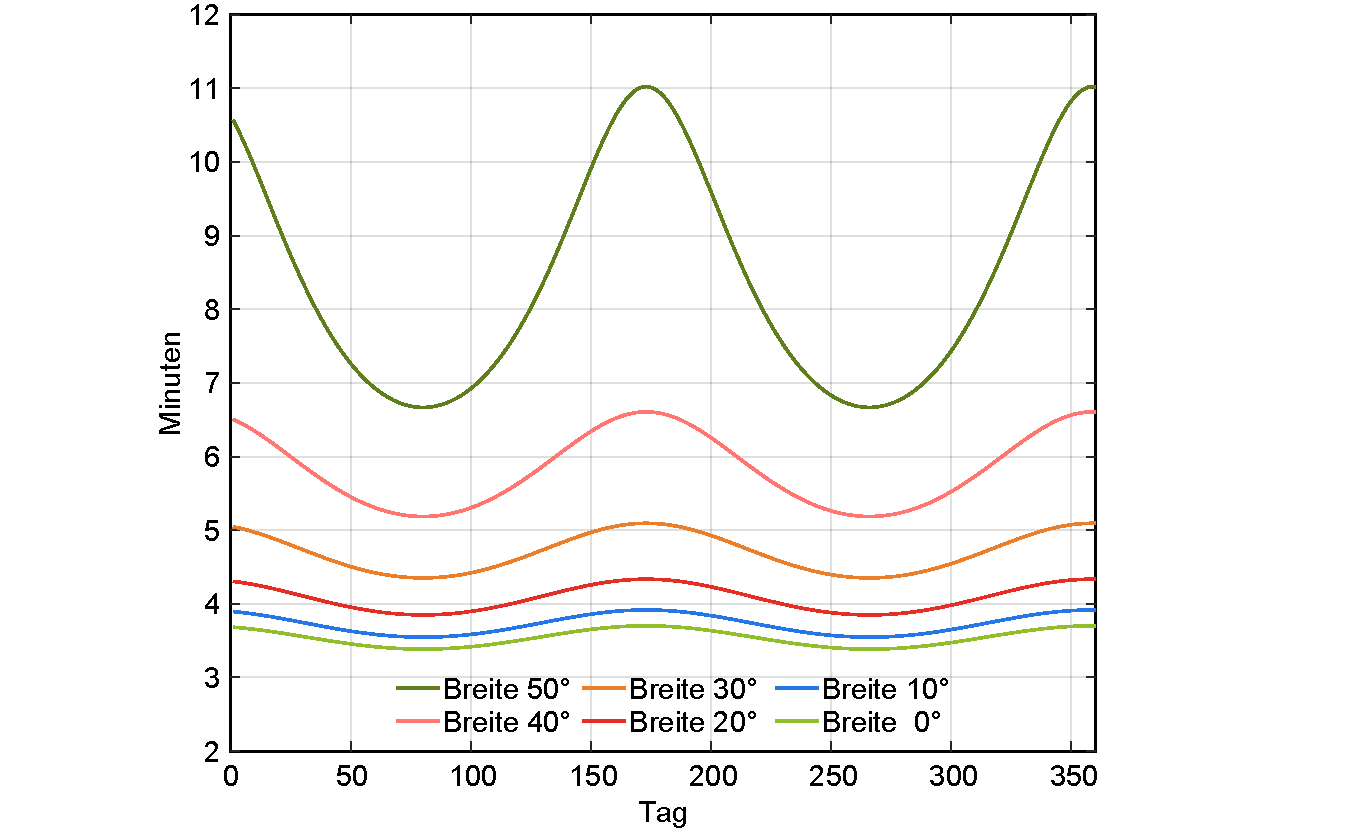
\includegraphics[width=\textwidth]{Tagbogenverlaengerung02.pdf}%
\caption[Tagbogenverl�ngerung durch Refraktion und scheinbaren Radius.]{Tagbogenverl�ngerung durch Refraktion und scheinbaren Radius im Laufe eines Jahres f�r verschiedene geographische Breiten nach \eqref{eq:hm_tagbogverl} (\mscr{} \mlhmref{TagbogenVerlaengerung.m}).}%
\label{abb:hm_tagbogenverl_nach_Delta_tau_A}%
\end{figure}
\figref{hm_tagbogenverl_nach_Delta_tau_A} (\mlhmref{TagbogenVerlaengerung.m}) zeigt sehr deutlich, dass die so berechneten Tagbogenverl�ngerungen bei gro�en geographischen Breiten\index{Breitengrad} und zu den Sonnenwenden am gr��ten sind, was unmittelbar einsichtig ist, wenn man sich die H�he der Sonne im Tagesverlauf f�r verschiedene Jahreszeiten vergegenw�rtigt. In \probref{hm_tageslauf_sonne} werden die H�he der Sonne im Tagesverlauf unter Ber�cksichtigung der Refraktion und der �ber den Tag ver�nderlichen Deklination mittels der Keplerl�sung berechnet und die Abweichung zur N�herung bestimmt.

Damit sind wir nun in der Lage, die Auf- und Untergangszeiten der Sonne in UT vollst�ndig f�r alle geographischen Breiten und Tage des Jahres in der lokalen Ortszeit WOZ anzugeben:
\begin{equation} \label{eq:hm_aufgangszeiten}
t_\text{A,U}(\lambda,\varphi,\delta(t_\text{d})) = 12\!:\!00\:\text{h UT} - \frac{\lambda}{15\degree} + \tau_\text{ ZGL}(\delta) \mp \abs{\tau_\text{ B}}(\varphi,\delta) \mp \abs{\Delta\tau_\text{B}}(\varphi,\delta) \,.
\end{equation}
Hierin ist $\delta\!=\!\delta(t_\text{d})$ als Funktion durch \eqref{eq:hm_delta_von_T_hash} gegeben und damit eine Funktion des bestimmten Tages eines Jahres.
F�r $\tau_\text{ ZGL}(\delta)$ kann im Prinzip jede der verschiedenen Formeln der Zeitgleichung benutzt werden.
\figref{hm_sonne_untergang_baabe} zeigt die nach \eqref{eq:hm_aufgangszeiten} berechneten Zeiten f�r den Sonnenaufgang und Sonnenuntergang, die Kulminationszeiten und die Tagesl�ngen f�r zwei Orte verschiedener geographischer Breiten.
Die Abweichungen zur numerischen L�sung bleiben im Mittel im Bereich von einer Minute. %(siehe dazu auch die \mscre \ref{mls:hm_tagbogenverl} und \ref{mls:hm_tageslauf_sonne}).
\begin{figure}%
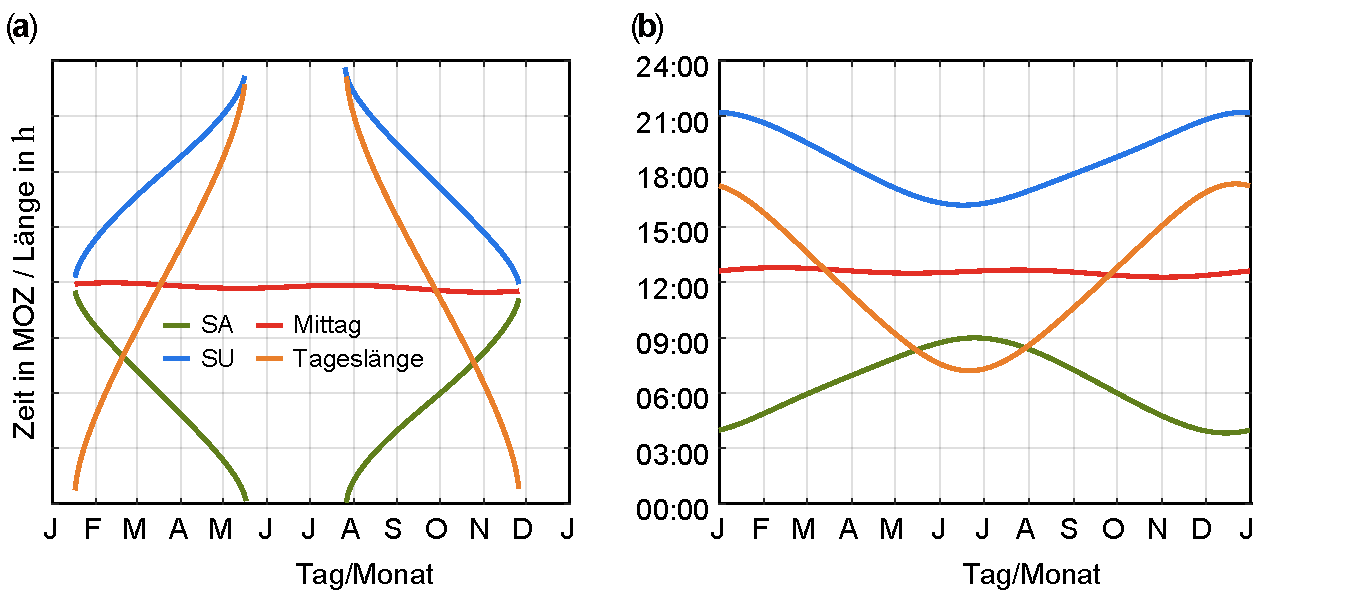
\includegraphics[width=\textwidth]{Sunrise02.pdf}\\%
\caption[Sonnenaufgang und -untergang f�r Troms� und Ushuaia.]{Sonnenaufgang und -untergang f�r \fa Troms�, Norwegen (Breite $69.8\degree$N und L�nge $19.0\degree$E) und \fb Ushuaia, Argentinien (Breite $54.8\degree$S, L�nge $68.3\degree$W). Die $x$-Achsen sind in Monaten angegeben: \anf{J}$=$Januar, \anf{F}$=$Februar, \anf{M}$=$M�rz, \ldots}%
\label{abb:hm_sonne_untergang_baabe}%
\end{figure}

\subparagraph{\textbf{Berechnung des Auf- bzw. Eintauchwinkels der Sonne}}
Zum Schluss wollen wir noch den Auf- \bzw Eintauchwinkel $\vartheta$ der Sonne in den Horizont berechnen.
Der Eintauchwinkel wird eine Funktion der Deklination und geographischen Breite sein.
Der Eintauchwinkel kann nach \figref{hm_verl_tagbogen_ref} wie folgt berechnet werden:
\begin{equation}
\tan\vartheta = \frac{\Delta h}{\Delta \mathcal{A}} \,.
\label{eq:hm_tan_vartheta}
\end{equation}
Unter Benutzung der Kettenregel erhalten wir
\begin{equation*}
\tan\vartheta = \frac{\D h}{\D \mathcal A} = \frac{\D h}{\D \tau}\frac{\D \tau}{\D \mathcal{A}} = \frac{\D h}{\D \tau} \lk \frac{\D \mathcal{A}}{\D \tau} \rk^{-1} \,.
\end{equation*}
Wir bilden die impliziten Ableitungen der Transformationsgleichung f�r $\sin h$ und $\sin \mathcal A$, sodass 
\begin{equation}
\frac{\D h}{\D \tau} = -\cos\delta\cos\varphi\sin\tau ~~\:\text{bzw.} ~~ \:\frac{\D \mathcal{A}}{\D \tau} = \frac{\cos\delta\cos\tau}{\cos\mathcal{A}}\,.
\label{eq:hm_dh_dtau}
\end{equation}
Formel \eqref{eq:hm_dh_dtau} in \eqref{eq:hm_tan_vartheta} eingesetzt ergibt
\begin{equation*}
\tan\vartheta = -\cos\varphi\cos\mathcal{A}_\text{A}\tan\tau_\text{A} \,.
\end{equation*}
Wir benutzen noch einmal die Transformationsformeln f�r $\cos\mathcal{A}$ und $\tan\tau$.
Mit $\cos\mathcal{A}\!=\!-\sin\delta/\cos\varphi$ eingesetzt in $\tan\tau\!=\!-\sin\mathcal{A}/(\tan\varphi\sin\delta)$ erhalten wir schlie�lich 
\begin{equation}
\tan\vartheta = \sqrt{\frac{\cos^2\varphi}{\sin^2\varphi} - \frac{\sin^2\delta}{\sin^2\varphi}} = \sqrt{\frac{\cos^2\delta}{\sin^2\varphi}-1} \,.
\label{eq:hm_tan_vartheta_2}
\end{equation}

\subparagraph{\textbf{Anwendung der Formeln f�r Sonnenauf- und -unterg�nge}}
Wir haben mit der Beziehung \eqref{eq:hm_aufgangszeiten} und mit \eqref{eq:hm_tan_vartheta_2} unser Ziel erreicht und zwei an jedem Ort der Erde und f�r jeden Tag des Jahres g�ltige \anf{Taschenrechnerformeln} erhalten.
W�hrend eines sommerlichen Familien-Ostseeurlaubs 2020 konnten wir die G�ltigkeit obiger Formel wenige Tage vor der Sommersonnenwende in Baabe ($\varphi\!=\!54.3591652\degree,\,\lambda\!=\!13.7061473\degree$) �berpr�fen.\footnote{Die Aufnahme wurde von Sylvia und Michael Kaschke mit einem ZEISS Batis Objektiv mit $\SI{135}{\milli\metre}$ Brennweite und einer Sony Alpha IIC am 10.\,6.\,2020 gemacht!}
Die beobachtete Aufgangszeit um 04:32:20 MESZ stimmt sehr gut mit den Berechnungen �berein (Tabelle \ref{tab:hm_beob_sonnenaufgang_baabe}).
Dies ist insbesondere bemerkenswert, da durch die Temperatur- und Druckvariation in der N�he des Horizonts die H�hen eines Himmelsobjektes um bis zu $0.3$\textdegree\ variieren k�nnen\cite{Meeus1998}.
Deswegen macht es auch keinen Sinn, die Aufgangszeiten wesentlich genauer als auf eine Minute zu berechnen. Unsere N�herungsformeln sind also gut anwendbar.
Signifikante Abweichungen bei diesen ergeben sich erst bei der Anwendung in gr��eren geographischen Breiten.
Generell gilt in der Himmelsmechanik, dass man zum einen mit hoher Genauigkeit (z.\,B. bei den Bahnparametern bzw. der Zeit in JD) rechnen muss, andererseits sollte man ber�cksichtigen, was �berhaupt bis zu welcher Genauigkeit beobachtet werden kann.
Kulminationen sind im Allgemeinen auf wenige Zeitsekunden, Planetenpositionen f�r Amateure auf ca. $10$ bis $20$ Bogensekunden und Aufg�nge wie oben beschrieben auf ca. eine Zeitminute genau beobachtbar.

\begin{table}%
\caption[Beobachtungen und Berechnungen des Sonnenaufgangs in Baabe.]{Beobachtungen und Berechnungen des Sonnenaufgangs in Baabe am 10.6.2020 (alle Zeiten in MESZ).}
\begin{tabular}{L{4cm}L{2.5cm}L{2.5cm}}
\hline\noalign{\smallskip}
  & Astrometrisch & Scheinbar \\
  &(Sonnenzentrum) & (Oberer Rand) \\
\noalign{\smallskip}\svhline\noalign{\smallskip}
JPL\cite{JPL2020} & 04:39:00 & 04:32:00 \\
Berechnet nach \eqref{eq:hm_tau_zgl} & 04:39:35 & 04:32:30 \\
N�herungsformel \eqref{eq:hm_ZGL21} & 04:39:50 & 04:32:10 \\
Beobachtet am 10.\,06.\,2020 & --- & 04:32:40 \\
\noalign{\smallskip}\hline\noalign{\smallskip}
\end{tabular}
\label{tab:hm_beob_sonnenaufgang_baabe}
\end{table}
Auch der Aufgangswinkel $\vartheta$ konnte vermessen werden.
Wenn man in Abb. \ref{eq:hm_sonnenaufgang_baabe_foto} die Anstiege f�r die eingezeichneten Regressionsgeraden bestimmt, so erh�lt man einen Winkel von $\vartheta_1\!=\!25.5$\textdegree\ f�r den oberen Rand der Sonne und $\vartheta_2\!=\!26.8$\textdegree{} f�r den unteren Rand.
Aus einer Rechnung im \mscr~\mlhmref{SonnenaufgangBaabe.m} findet man unter Verwendung der Refraktionsformeln \eqref{eq:hm_Normalrefraktion1} \bzw \eqref{eq:hm_Normalrefraktion2} Werte um $\vartheta\!=\!24.6$\textdegree.
Im Rahmen der Messgenauigkeit stimmt das gut mit unserer Messung �berein.
Aus den unterschiedlichen gemessenen Winkeln wird aber auch deutlich, dass die Refraktion im Bereich $0$\textdegree\ bis $2$\textdegree\ nicht als konstant angenommen werden kann. 
\begin{figure}%
\includegraphics[width=\textwidth]{SunRiseBaabe.pdf}%
\caption[Verlauf des Sonnenaufgangs an der sommerlichen Ostsee.] {Verlauf des Sonnenaufgangs an der sommerlichen Ostsee.}%
\label{eq:hm_sonnenaufgang_baabe_foto}%
\end{figure}
In den \textbf{�bungen} \ref{prob:hm_abflachung_sonne} bis \ref{prob:hm_sonnenaufgang_mars} haben wir einige Beispiele zur Berechnung von Aufgangssituationen auf der Erde bzw. auf einem anderen Planeten vorgesehen.
Die Methodik, die wir bei der Erde verwendet haben, ist auch auf solche F�lle �bertragbar.
In der \probref{hm_analytic_sunrise} wird nach \cite{Reinsch2003} eine Methode dargestellt, mit der eine zumindest f�r die Breitengrade zwischen $25\degree$ und $65\degree$ brauchbare analytische Formel f�r den Sonnenaufgang hergeleitet wird.

\subsubsection{Konstruktion von Sonnenuhren}\index{Sonnenuhr}\label{kap:sonnenuhren}

Mit unserem Wissen �ber die Berechnung der Koordinaten der  Sonne als Funktion und der Zeitgleichung k�nnen wir auch an die Berechnung von Sonnenuhren gehen.
Sonnenuhren sind die �ltesten Zeitmesser auf der Erde.\footnote{In der Literatur wird debattiert, ob Wasser- \bzw Sanduhren noch �lter sind. Diese Uhren k�nnen aber nur Intervalle messen und bestimmen die Zeit nicht in Bezug zur astronomisch definierten Zeit.}
Es gibt ausgezeichnete und umfangreiche Literatur zu diesem Thema \cite{Meyer2008, Kloeckl2017}, weshalb wir uns hier auf die Grundprinzipien beschr�nken und ansonsten auf die Literatur bzw. die �bungen verweisen.

\subparagraph{\textbf{Grundprinzip und Begriffe einer Sonnenuhr}}

Mit einer Sonnenuhr wird durch die Sonne ein (Schatten-)Bild eines Stabes oder eines anderen Objektes auf einem geeignet zu konstruierenden Ziffernblatt erzeugt (\figref{hm_sundial_RvB}).
Aus dem Stand der Sonne bzw. deren Schatten kann dann die Tageszeit (Uhrzeit) unmittelbar abgelesen werden.
Die Tageszeit kann je nach Gestaltung der Sonnenuhr bzw. ihres Zifferblatts als Wahre Ortszeit (WOZ), \gls{moz} (MOZ) oder Zonenzeit (MEZ) angezeigt werden.
Mit Hilfe von Sonnenuhren lassen sich auch jahreszeitliche Informationen ablesen, z.B. das Datum, Sonnenwenden und �quinoktien.
Wir wollen dabei folgende Begriffe aus der \gls{gnomonik} (Lehre von den Sonnenuhren) verwenden (\figref{hm_sundial06}):

\begin{figure}%
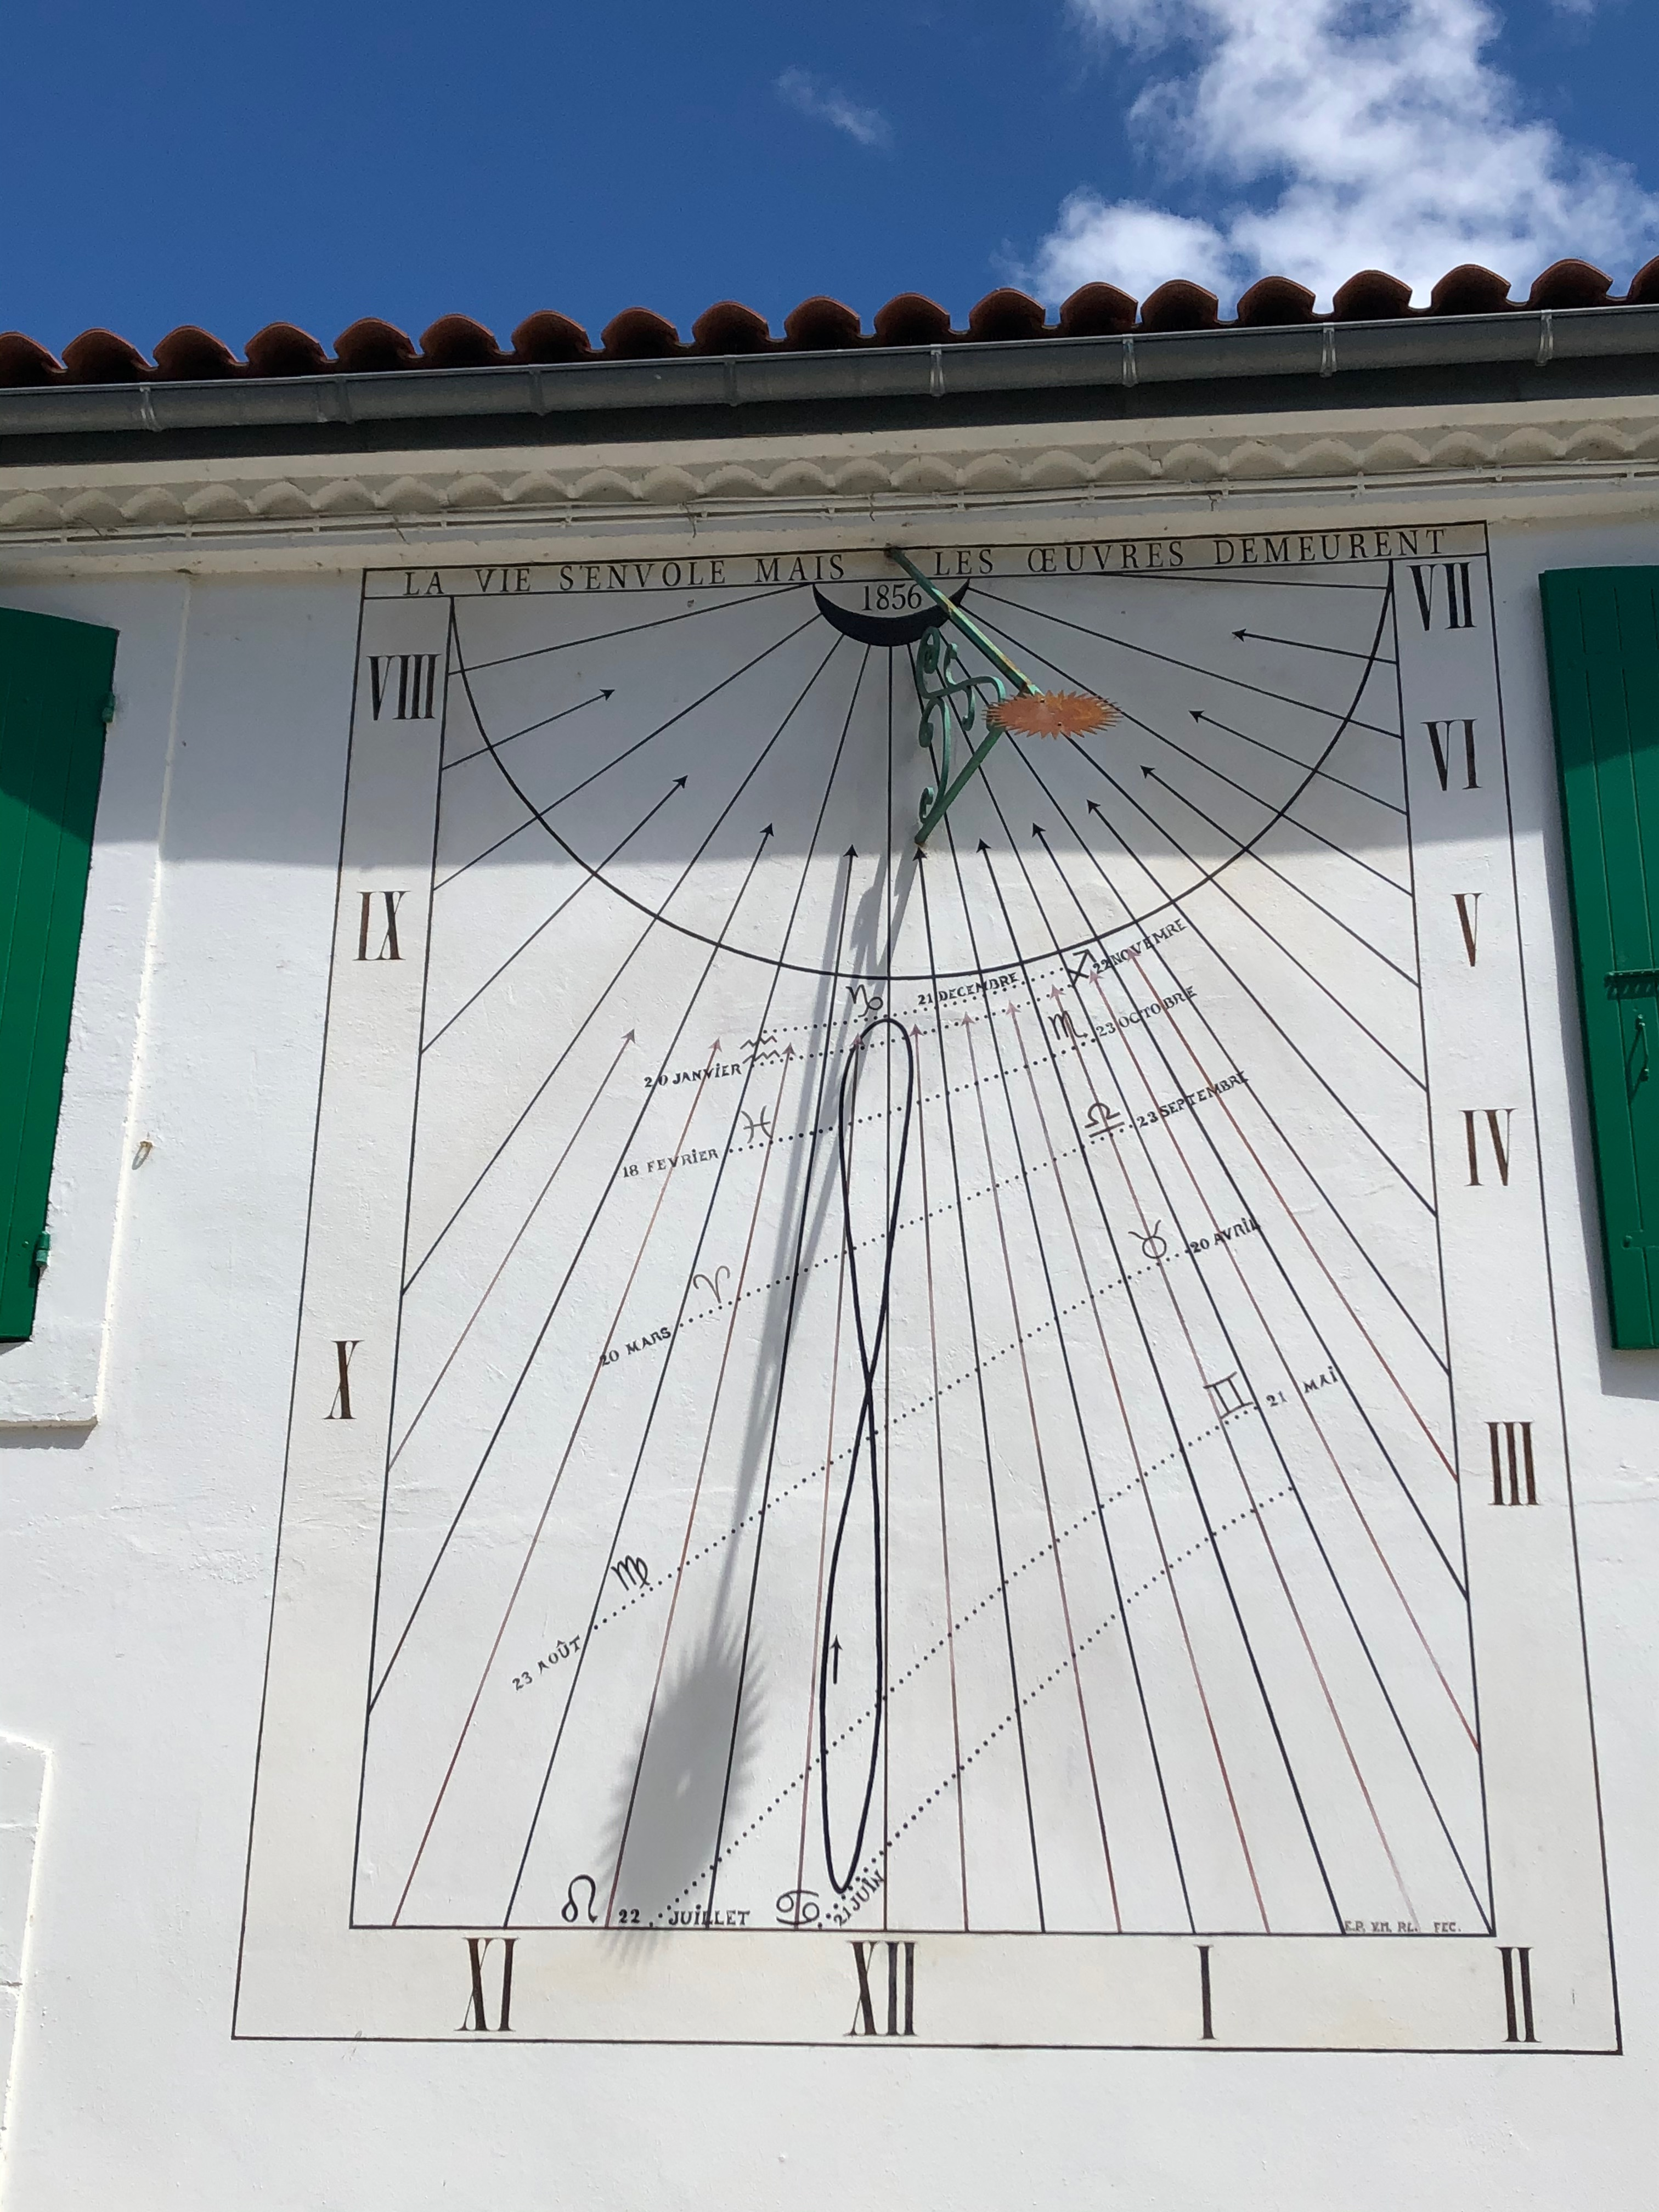
\includegraphics[width=0.4\textwidth]{SunDial.jpg}%
\caption[Sonnenuhr am B�rgermeisteramt in St. Pierre d'Ol�ron in Frankreich.]{Sonnenuhr am B�rgermeisteramt in St. Pierre d'Ol�ron in Frankreich. Die Inschrift auf der Uhr sagt: La vie s'envole, mais les oeuvres demeurent. (Wir bedanken uns bei Rudolf von B�nau f�r das Bild.)}%
\label{abb:hm_sundial_RvB}%
\end{figure}

\renewcommand*{\arraystretch}{1}
\begin{longtable}{L{1.5 cm}L{0.5 cm}L{8.5 cm}}
\noalign{\smallskip}\svhline\noalign{\smallskip}
Begriff & &Erkl�rung \\
\noalign{\smallskip}\svhline\noalign{\smallskip}
\endhead
  \textit{\gls{gnomon}} & & Schattenwerfender Stab.\index{Gnomon}\\ 
  \textit{\gls{nodus}} & & Spitze des Gnomons\index{Nodus} (auch Auge genannt).\\ 
  \textit{\gls{lineatur}} & & Menge der vom Gnomon oder Nodus geworfenen Schatten auf einer Ziffernblattebene\index{Lineatur}, auf der die Zeit abgelesen werden kann.\\
\noalign{\smallskip}\svhline\noalign{\smallskip}
\end{longtable}
\renewcommand*{\arraystretch}{1}

\begin{figure}%
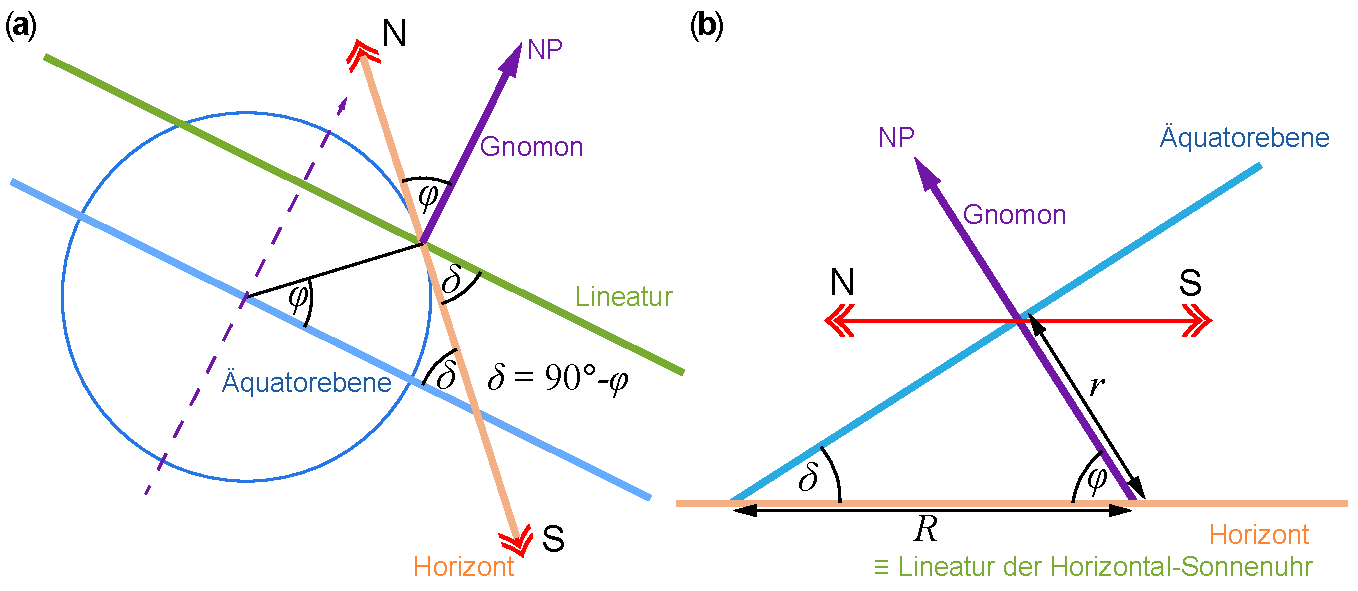
\includegraphics[width=\textwidth]{Sonnenuhr06.pdf}%
\caption[Grundprinzip einer �quatorial- und einer Horizontal-Sonnenuhr.]{Grundprinzip von Sonnenuhren. \fa �quatorial-Sonnenuhr und \fb Horizontal-Sonnenuhr. $\varphi$ ist die geographische Breite, NP der Himmelsnordpol und N, S die Nord- \bzw S�drichtung in der Horizontebene.}%
\label{abb:hm_sundial06}%
\end{figure}

\subparagraph{\textbf{�quatoriale (Polstab-)Sonnenuhr}}

\begin{figure}%
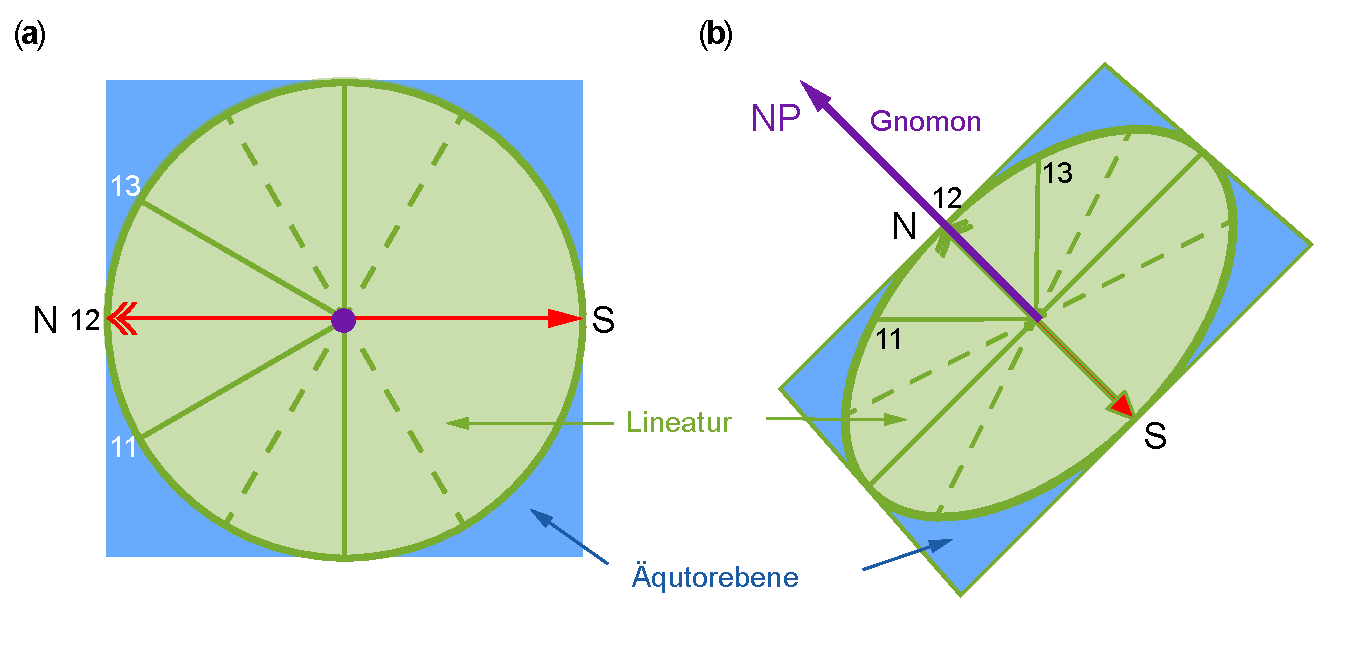
\includegraphics[width=\textwidth]{Sonnenuhr01.pdf}%
\caption[Prinzip und Ausf�hrung einer �quatorial-Sonnenuhr.]{Prinzip und Ausf�hrung einer �quatorial-Sonnenuhr. \fa Draufsicht auf Lineaturebene (parallel zur �quatorebene), \fb Schr�gansicht.}%
\label{abb:hm_sundial01}%
\end{figure}

Diese Sonnenuhr ist die einfachste Sonnenuhr, man findet sie h�ufig in G�rten oder Parks.
Bei ihr liegt das Ziffernblatt mit der Lineatur in einer Ebene, die parallel zur �quatorebene ist.
Die Lineatur ist gleichm��ig aufgeteilt und der Schattenstab steht senkrecht auf dem Ziffernblatt und zeigt damit zum Himmelsnordpol (\figref{hm_sundial02}). \\
Bei positiver Deklination der Sonne kann der Schatten direkt auf dem Ziffernblatt abgelesen werden, bei negativen Deklinationen m�sste das Ziffernblatt transparent sein, da die Sonne von unten den Stab beleuchtet.
Man hilft sich, indem man entweder das Ziffernblatt transparent macht oder als halbkreisf�rmiges Band gestaltet. \\
Die Lineatur ist relativ zur Nordrichtung als Schatten per Definition durch den Stundenwinkel $\tau$ gegeben, den wir im Folgenden mit $\sigma_\text{A}$  bezeichnen wollen. Will man eine Beziehung der Lineatur zur b�rgerlichen Zeit herstellen, so ist unter Annahme einer mittleren Sonne die Lineatur durch

	\begin{align}
				\sigma_\text{A} = \text(MOZ) \frac{15\degree}{\mathrm{h}}+\lambda - \text{Z}\cdot15\degree \label{eq:hm_sundial01}
		\end{align}
gegeben, worin die MOZ wie in \kap{hm_zeitdefinition} definiert die mittlere Ortszeit in Stunden (h), $\lambda$ die geographische L�nge und Z die Zeitzone bedeuten.\\

\subparagraph{\textbf{Horizontal-Sonnenuhr}}

\begin{figure}%
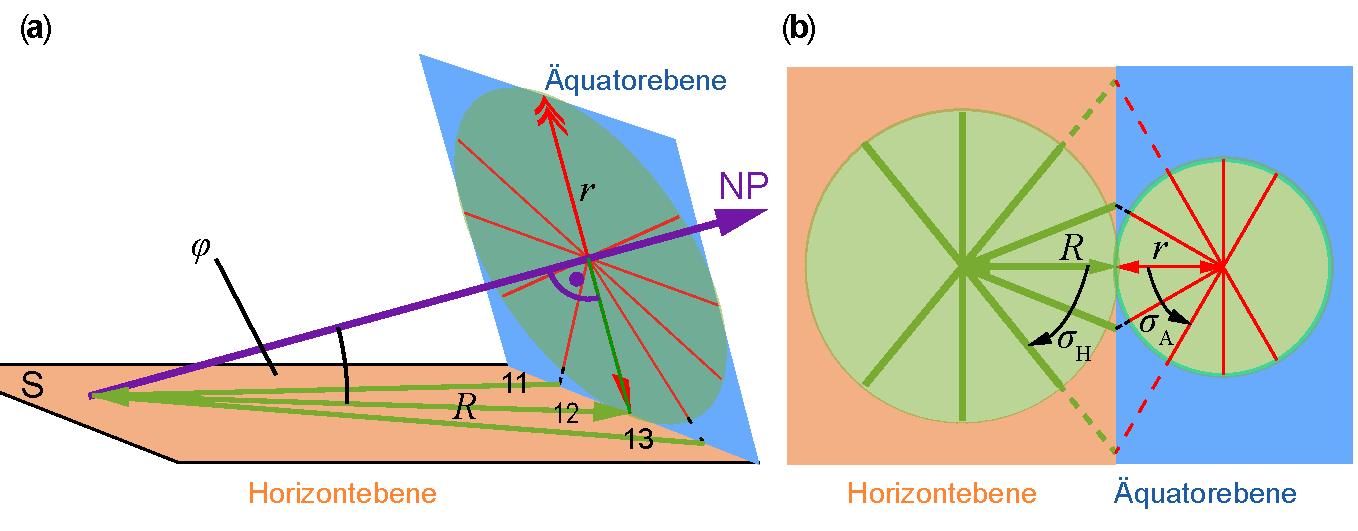
\includegraphics[width=\textwidth]{Sonnenuhr03.pdf}%
\caption[Prinzip der Horizontal-Sonnenuhr.]{\fa Prinzip der Horizontal-Sonnenuhr und \fb Berechnungsgrundlage der Lineatur. $R$ ist hier Radius des Ziffernblatts der Horizontal-Sonnenuhr, $r$ der Radius des Ziffernblatts der �quatorial-Sonnenuhr.}%
\label{abb:hm_sundial02}%
\end{figure}

\begin{figure}%
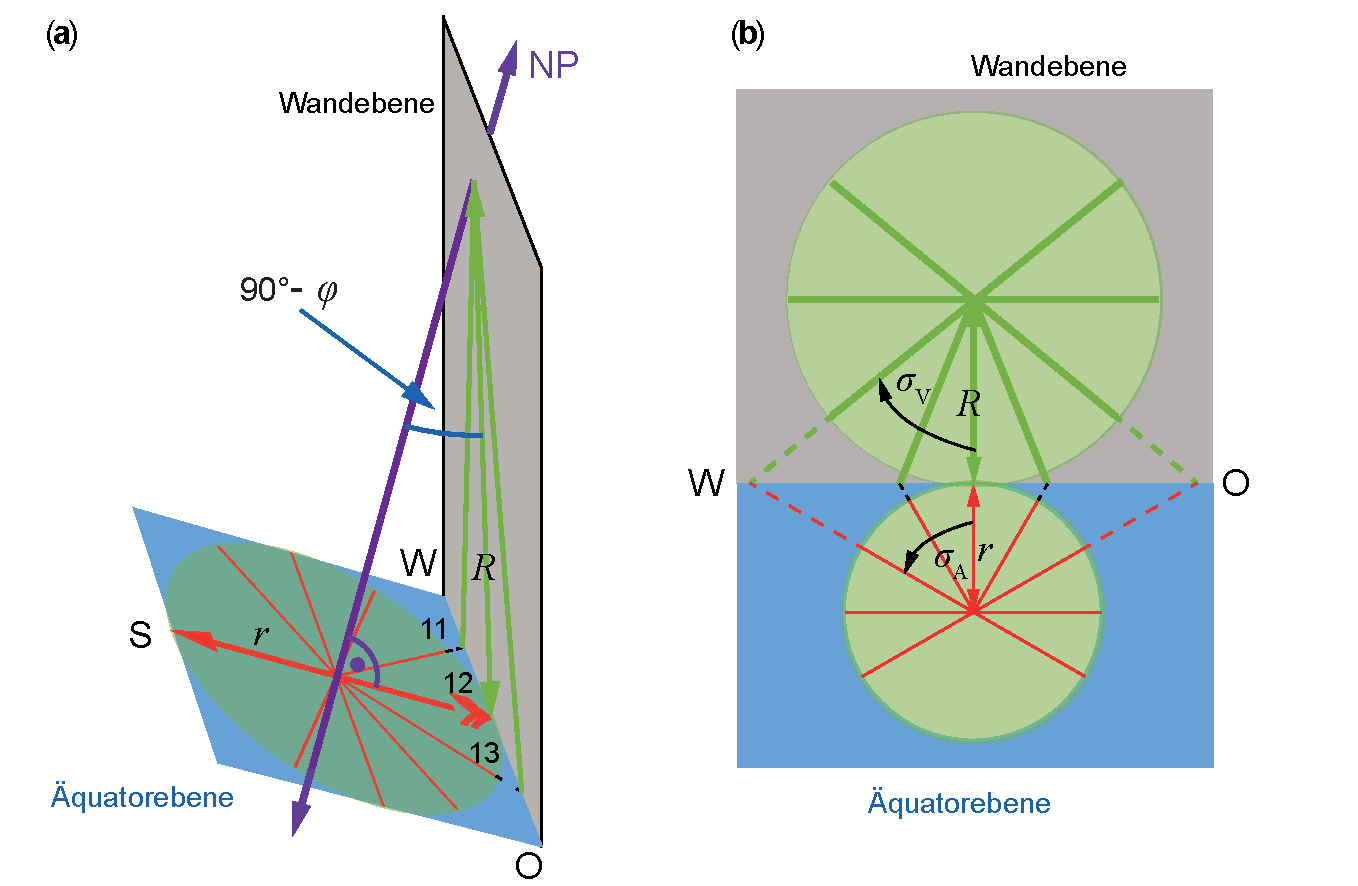
\includegraphics[width=\textwidth]{Sonnenuhr04.pdf}%
\caption[Prinzip der Vertikal-Sonnenuhr.]{\fa Prinzip der Vertikal-Sonnenuhr und \fb Berechnungsgrundlage der Lineatur bei O-W-Ausrichtung der Wand.}%
\label{abb:hm_sundial04}%
\end{figure}

Diese Sonnenuhr findet man auf ebenen Fl�chen, sie sind sehr einfach zu bauen, daf�r ist die Lineatur etwas komplizierter.
Die Konstruktion der Lineatur einer solchen Horizontal-Sonnenuhr ergibt sich aus \figref{hm_sundial02}. \\
Der Schattenstab ist wieder zum Himmelsnordpol ausgerichtet, er bildet also zwischen Horizont- und Ziffernblattebene den Winkel $\varphi$, dessen Gr��e gleich der geographischen Breite des Aufstellungsortes entspricht.
Aus \figref{hm_sundial02} erkennt man, dass die Lineatur nicht mehr gleichm��ig ist.
Sie ergibt sich gem�� einfacher geometrischer �berlegungen zu
		\begin{align}
				\tan \sigma_\text{H} = \frac{r}{R}\,\tan\sigma_\text{A}  = \sin\varphi\,\tan\sigma_\text{A}\,. \label{eq:hm_sundial02}
		\end{align}
$\sigma_\text{H}$ ist hier der Winkel zwischen der Linie f�r die aktuelle Zeit und der 12:00 Stunden-Linie auf dem horizontalen Ziffernblatt, $\sigma_\text{A}$ der entsprechende Winkel auf dem �quatorialen Ziffernblatt.\\
\subparagraph{\textbf{Vertikal-Sonnenuhr}}
Diese Sonnenuhr findet man h�ufig an Hausw�nden.
Ihre Konstruktion ist f�r eine in West-Ost-Richtung verlaufende Wand v�llig analog der Horizontal-Sonnenuhr, nur erfolgt hier die Projektion nicht auf den Horizont, sondern auf eine dazu senkrechte Ebene. Die Uhr stellt quasi eine um $90\degree$ gedrehte Horizontal-Sonnenuhr dar, sodass wir folgende Beziehung erhalten:
		\begin{align}
				\tan\sigma_\text{V}= \sin(90\degree - \varphi)\,\tan\sigma_\text{A} = \cos\varphi\,\tan\sigma_\text{A} \,. \label{eq:hm_sundial03}
		\end{align}
Etwas schwieriger ist die Berechnung, wenn die Wand um einen Winkel $\alpha$  gegen die Ost-West-Achse gedreht ist, was sicher h�ufig vorkommt (\figref{hm_sundial05}). Diese Berechnung wird in \probref{hm_VertikalAnalemmaSonnenuhr} ausgef�hrt. 

\subparagraph{\textbf{Analemmatische Sonnenuhren}}
Bisher haben wir bei der Berechnung der Lineatur die Zeitgleichung nicht ber�cksichtigt, \dh wir haben nach \eqref{eq:hm_sundial01} ein Ziffernblatt f�r die MOZ berechnet.
Da aber die WOZ von der MOZ bis zu $\pm 15 \,\mathrm{min}$ variiert, wollen wir uns eine Sonnenuhr �berlegen, die die ZGL und die unterschiedliche Deklination der Sonne im Laufe eines Jahres ber�cksichtigt. Eine solche Sonnenuhr steht \zb vor dem Galilei-Museum in Florenz (\figref{hm_sundial07}). 

\begin{figure}%
\includegraphics[width=\textwidth]{Sonnenuhr07.pdf}%
\caption[Analemmatische Sonnenuhr vor dem Galilei-Museum in Florenz.]{\fa Analemmatische Sonnenuhr vor dem Galilei-Museum in Florenz (Florenz, Italien) und \fb Konstruktionsprinzip. Nodus (Nd), Nodus-Schattenpunkt (SP), Azimut ($\mathcal{A}$), H�he $H$ des Schattenstabes und H�he $h$ der Sonne (S) sind dargestellt. }%
\label{abb:hm_sundial07}%
\end{figure}

Bei dieser Sonnenuhr erfolgt das Ablesen der Zeit nicht durch eine Schattenlinie, sondern durch den Punktschatten eines Nodus (Nd), der zu jedem Datum einen anderen Punkt des Ziffernblatts beschattet. Der Schattenstab der H�he $H$ muss daher nicht auf den Himmelspol ausgerichtet sein, da es nur auf den Schatten des Nodus ankommt. Wir betrachten die Position $\vec{r}_\text{n}$ des Nodusschattens (SP) in der Horizont-Ziffernblattebene ($x$-$y$-Ebene), wobei $\vec{n}$ die Richtung zum Nodus ist und $\vec{s}$ die Richtung vom Nodus-Schattenpunkt SP zur Sonne S.
Dann gilt (\figref{hm_sundial07}b:
		\begin{align}
				\vec{r}_\text{n} &= \vec{n}+q\,\vec{s} \,, ~~~~ \vec{r}_\text{n}\,\veceZ = 0 = \vec{n}\,\veceZ + q\,\vec{s}\,\veceZ \,, ~~~~~q = -\frac{\vec{n}\,\veceZ}{\vec{s}\,\vec{e}_z} \,, \nonumber \\
				\longrightarrow \vec{r}_\text{n} &= \vec{n}-\frac{\vec{n}\,\veceZ}{\vec{s}\,\veceZ}\vec{s} = \frac{(\vec{s}\,\veceZ)\,\vec{n}-(\vec{n}\,\veceZ)\,\vec{s}}{\vec{s}\,\veceZ} = \frac{\veceZ\times(\vec{n}\times\vec{s})}{\vec{s}\,\veceZ} \,. \label{eq:hm_sundial04}
		\end{align}
Man erkennt aus \eqref{eq:hm_sundial04}, dass die Abbildung der Sonnenrichtung $\vec{s}$ auf das Ziffernblatt nichtlinear ist, da $\vec{s}$ in Z�hler und Nenner steht.
Im Fall der Sonnenuhr von Florenz ist die H�he des Nodusstabes $H \approx \SI{3}{\metre}$.
Im KOS von \figref{hm_sundial07} ergeben sich die Vektoren $\veceZ,\, \vec{n}$ und der Richtungsvektor zur Sonne $\vec{s}$ zu:
	\begin{align*}
                \veceZ&= 
                \begin{pmatrix}
                0 \\
                0 \\
                1
                \end{pmatrix}\,, ~~~~~
                \vec{n}= 
                \begin{pmatrix}
                0 \\
                0 \\
                H
                \end{pmatrix} ~~~~\text{und}~~~~
                \vec{s}= 
                \begin{pmatrix}
                s_\text{x} \\
                s_\text{y} \\
                s_\text{z}
                \end{pmatrix} = 
                \begin{pmatrix}
               	\cos h \, \cos\mathcal{A} \\
               	\cos h \, \sin\mathcal{A} \\
               	\sin h 
								\end{pmatrix}  \,. 
	\end{align*}
Hier haben wir Azimut $\mathcal{A}$ und der H�he $h$ der Sonne verwendet, die man \zb wie in \kap{zeitgleichung} beschrieben zu beliebigen Zeiten $t$ eines Jahres berechnen kann. Die Schattenl�nge und Richtung ergeben sich dann zu (siehe auch \probref{hm_VertikalAnalemmaSonnenuhr}):
		\begin{align}
				\vec{r}_\text{n} = \frac{H}{s_\text{z}(t)}
				\begin{pmatrix}
				-s_\text{x}(t) \\
				-s_\text{y}(t) \\
				0
				\end{pmatrix} = H 
				\begin{pmatrix}
				-\cot\lek h(t)\, \cos\mathcal{A}(t) \rek \\
				-\cot\lek h(t)\, \sin\mathcal{A}(t) \rek \\
				0
				\end{pmatrix}\,. \label{eq:hm_sundial06}
		\end{align}
Man kann mit den Ergebnissen der Rechnung \zb die Linien gleichen Datums (\bzw gleicher Deklination) auftragen und darauf die Uhrzeit markieren.
Alternativ kann man die Stundenlinien (\dh die Punkte f�r eine feste Uhrzeit) im Laufe eines Jahres auftragen.
Dies ist Gegenstand der \probref{hm_VertikalAnalemmaSonnenuhr}.\\
Wir m�chten auch noch auf die relativ einfach und zugleich interessant konstruierte �quatorial-analemmatische Sonnenuhr von Hermann Zeuner \cite{Zeuner2011} verweisen, die in der \probref{hm_Aalener_Sonnenuhr} (Zusatz�bung) n�her betrachtet werden kann.

\subsection{Berechnung von Planetenbahnen}\index{Planetenbahnen}\label{kap:hm_bahnen_hk_ss}

\subsubsection{Berechnung der Planetenbahnen mit Gau�schen Vektoren} \label{kap:hm_bahnen_hk_PQR}
Wir k�nnen nun analog zum Vorgehen in \kapitel{erdbahn} auch Bahnen mit einer Bahnneigung~$i$ zur Ekliptik (\figref{hm_planetenbahnen_rel_ekliptik}) behandeln und damit die Berechnung der Planetenbahnen unseres Sonnensystems in Angriff nehmen.
Dazu m�ssen die Bahnkoordinaten $r$, $\upsilon$, die aus der Kepler-Gleichung berechnet werden, auf die Ekliptik projiziert (\anf{reduziert}) werden.
Diese Projektion ist als eine der Koordinatentransformationen in Tabelle \ref{tab:hm_Umrechung_KOS} gelistet.
Wir wollen hier aber noch einen anderen, sehr eleganten Weg aufzeigen.
Die Abbildung der Vektoren zwischen beiden KOS kann durch eine Matrix-Transformation wie folgt beschrieben werden:
\begin{equation}
\vec{r}_\text{Ekl} = \lk\begin{array}{c} x\\ y\\ z \end{array}\rk = \mathbb{U}\cdot \vec{r}_\text{Bahn} = \lk\begin{array}{ccc} \vec{P} & \vec{Q} & \vec{R} \end{array}\rk \vec{r}_\text{Bahn} = \mathbb{U} \cdot \lk\begin{array}{c} r\cos\upsilon\\ r\sin\upsilon\\ 0 \end{array}\rk ~. \label{eq:hm_gauss_ansatz}
\end{equation}
Die Matrix $\mathbb{U}$ setzt sich aus drei Spalten-Vektoren $\vec{P}$, $\vec{Q}$, $\vec{R}$, den sogenannten Gau�schen\footnote{Johann Carl Friedrich Gau� (auch oft Gauss) (1777 -- 1855) war ein deutscher Mathematiker, Astronom, Geod�t und Physiker. Wegen seiner �berragenden wissenschaftlichen Leistungen galt er bereits zu seinen Lebzeiten als \textit{Princeps mathematicorum - F�rst der Mathematiker}. Seine Arbeiten erstreckten sich von vielen Feldern der Mathematik und Physik auch auf angewandte Gebiete, zum Beispiel der Landesvermessung und der elektromagnetischen Telegraphie.}\indexp{Gau�, Johann Carl Friedrich} Vektoren, zusammen, deren Herleitung im Detail in Beispiel \ref{bsp:herleitung_gauss_vek} beschrieben wird.
Die Gau�schen Vektoren\index{Vektoren!Gau�sche} stellen f�r eine Bahn jeweils Konstanten (f�r das betrachtete �quinoktium) dar, da sie nur von den Bahnparametern abh�ngen:
\begin{align}
\begin{split}
\vec{P} &= \lk\begin{array}{c} + \cos\omega\cos\Omega - \sin\omega\cos i\sin\Omega\\ + \cos\omega\sin\Omega + \sin\omega\cos i\cos\Omega\\ + \sin\omega\sin i \end{array}\rk \,, \\
\vec{Q} &= \lk\begin{array}{c} -\sin\omega\cos\Omega - \cos\omega\cos i\sin\Omega\\ -\sin\omega\sin\Omega + \cos\omega\cos i\cos\Omega\\ + \cos\omega\sin i \end{array}\rk \,, \\
\vec{R} &= \lk\begin{array}{c} + \sin i\sin\Omega\\ -\sin i\cos\Omega\\ + \cos i \end{array}\rk \,. 
\end{split} \label{eq:hm_gauss_vektoren}
\end{align}
Der Vorteil ist offensichtlich.
Wenn man die zeitliche Entwicklung der Bahnkoordinaten berechnet hat, braucht man f�r die Projektion auf die Ekliptik die Matrix $\mathbb{U}$ nur einmal auszurechnen.
Diese Methodik ist dann sehr effizient, wenn man viele Koordinaten �ber viele St�tzstellen berechnen muss oder die Geschwindigkeiten des Himmelsk�rpers braucht.

%BEISPIEL 5 %%%%%%%%%%%%%%%%%%%%%%%%%%%%%%%%%%%%%%%%%%%%%%%%%%%%%%%%%%%%%%%%%%%%%%%%%%%%%%%%%%
\begin{example}{\textbf{\textit{Herleitung der Gau�schen Vektoren}}}
Wir wollen die Gau�schen Vektoren nach \eqref{eq:hm_gauss_vektoren} herleiten.
Wir starten dabei von den kartesischen Koordinaten der Bahnebene und wollen daraus die heliozentrischen kartesischen Koordinaten herleiten.
Dazu benutzen wir f�r die Transformation zwischen den beiden KOS die Drehmatrizen mit den entsprechenden Bahnparametern.
\medskip\\
Die gesamte Transformation kann man als Abfolge dreier Rotationen betrachten:
\begin{enumerate}[(1)]
	\item \emph{Drehung in der Bahnebene um die $z$-Achse zur Ber�cksichtigung der Perihellage $\omega$ relativ zum aufsteigenden Knoten}\\
	Der Ausgangsvektor ist gegeben als
	\begin{align*}
	\vec{r}_0 = \lk\begin{matrix} r \cos \upsilon \\ r \sin \upsilon \\ 0 \end{matrix} \rk\,.
\end{align*}
	Nach der Drehung um $-\omega$ zeigt die neue $x$-Achse in Richtung des Knotens.
        Die Drehung wird beschrieben durch 
	\begin{align*}
	\vec{r}_1\:=\:\mathbb{R}_z(-\omega)\, \vec{r}_0 = 
	\lk\begin{matrix} +\cos \omega &\; -\sin \omega &\; 0 \\
	                     +\sin \omega &\; +\cos \omega &\; 0 \\
                          0         &\;     0        &\; 1 \end{matrix} \rk \cdot \vec{r}_0 \ \:=\: 
													r \lk\begin{matrix} \cos u \\ \sin u \\ 0 \end{matrix} \rk 
\end{align*}
mit $u\!=\!\upsilon+\omega$.
	\item \emph{Drehung der Bahnebene um die $x$-Achse in die Ekliptikebene zur Korrektur der Bahnneigung $i$ gegen�ber der Ekliptik}
\begin{align*}
	\vec{r}_2\:=\:\mathbb{R}_x(-i)\cdot \vec{r}_1 =
	\lk\begin{matrix} 1 &\; 0 &\; 0 \\ 0 &\; +\cos i &\; -\sin i \\ 0 &\; +\sin i &\; +\cos i \end{matrix} \rk \cdot \vec{r}_1 \ =
	r \lk\begin{matrix} \cos u \\ \sin u \cos i\\ \sin u \sin i \end{matrix} \rk ~\,.
\end{align*}
	\item \emph{Drehung um die $z$-Achse in der Ekliptikebene zur Ber�cksichtigung der Knotenlage $\Omega$ relativ zum Fr�hlingspunkt} $\vernal$
	\begin{align*}
	\vec{r}_3 = \mathbb{R}_z(-\Omega)\cdot \vec{r}_2 &=
	\lk\begin{matrix} +\cos \Omega &\; -\sin \Omega &\; 0 \\
	                     +\sin \Omega &\; +\cos \Omega &\; 0 \\
                          0         &\;     0        &\; 1 \end{matrix} \rk\cdot \vec{r}_2 \\
        &= r\,\lk\begin{matrix} \cos u \cos \Omega - \sin u \cos i \sin \Omega \\ \cos u \sin \Omega - \sin u \cos i \cos \Omega \\ \sin u \sin i \end{matrix} \rk \,.
\end{align*}
\end{enumerate}
Man kann die Gesamttransformation nat�rlich auch mit einer Matrix $\mathbb{U} (-\omega,-i,-\Omega)\!=\! \mathbb{R}_z(-\Omega) \mathbb{R}_x(-i) \mathbb{R}_z(-\omega)$ beschreiben.
Durch Ausmultiplizieren findet man
\begin{align*}
\mathbb{U} = \lk
\begin{matrix}
       + \cos\omega\cos\Omega - \sin\omega\cos i\sin\Omega &\; -\sin\omega\cos\Omega - \cos\omega\cos i\sin\Omega &\; + \sin i\sin\Omega \\
       + \cos\omega\sin\Omega + \sin\omega\cos i\cos\Omega &\; -\sin\omega\sin\Omega + \cos\omega\cos i\cos\Omega &\;- \sin i\cos\Omega \\
			 + \sin\omega\sin i                                  &\; + \cos\omega\sin i                                 &\; + \cos i \end {matrix} \rk \,.
\end{align*}
Die Spalten dieser Matrix $\mathbb{U}$ entsprechen nun genau den Gau�schen Vektoren $\vec{P},\,\vec{Q},\,\vec{R}$ in \eqref{eq:hm_gauss_vektoren}.
Man kann leicht zeigen, dass die Gau�schen Vektoren Einheitsvektoren sind.
Diese Einheitsvektoren spannen ein sogenanntes \textit{kartesisch-perifokales Koordinatensystem}\index{Koordinatensystem!perifokales} auf. 
Dieses ist dadurch definiert, dass dessen Ursprung weiterhin im Nullpunkt des Zentralk�rpers (z.\,B.\, der Sonne $\astrosun$) liegt und dessen $x,y$-Ebene die Bahnebene des durch die Bahnparameter gegebenen Himmelsk�rpers ist \cite{Walter2018}.
Der Vektor $\vec{R}$ zeigt dann logischerweise in Richtung des Drehimpulses  $\vec{L}$ und der Vektor $\vec{P}$ in Richtung des Laplace-Vektors $\vec{e}$. \\ 
\end{example}
%BEISPIEL %%%%%%%%%%%%%%%%%%%%%%%%%%%%%%%%%%%%%%%%%%%%%%%%%%%%%%%%%%%%%%%%%%%%%%%%%%%%%%%%%%
Dem aufmerksamen Leser wird nicht entgangen sein, dass die hier eingef�hrten Winkel eine gro�e �hnlichkeit mit den Euler-Winkeln\index{Euler-Winkel} aus Kapitel 1.4.2.2 (Band I) haben, die wir beim starren K�rper eingef�hrt haben, ja diesen auf  Grund der Bildungsvorschrift sogar entsprechen. Wir empfehlen dem Leser nachzuvollziehen, dass folgende �quivalenzen gelten:
\begin{longtable}{p{0.33\textwidth}p{0.05\textwidth}p{0.33\textwidth}}
\hline\noalign{\smallskip}
Starrer K�rper & &Himmelsmechanik \\
Euler-Winkel & &Bahnparameter \\
\hline\noalign{\smallskip}
$\varphi$ & &$\omega$ \\
$\vartheta$ & &$i$\\
$\psi$ & &$\Omega$
%\noalign{\smallskip}\hline\noalign{\smallskip}
\end{longtable} \label{bsp:herleitung_gauss_vek}
\medskip

In den \mscren \mlhmref{InnerePlaneten.m} \bzw \mlhmref{AeusserePlaneten.m} sind die Rechnungen f�r die inneren und �u�eren Planeten ausgef�hrt (Ergebnisse in \figref{hm_proj_bahnen_innere_pl} und \figref{hm_bahnen_aussere_pl}).
Aus der Berechnung der Bahnen f�r die �u�eren Planeten f�r den Zeitraum 1920--2020 k�nnen wir auch sehen, dass es Jahre gab, in denen selbst zu Zeiten, als Pluto noch ein \anf{vollwertiger} Planet war, Neptun wegen der Exzentrizit�t der Pluto-Bahn der am weitesten von der Sonne entfernte Planet war.

Wegen der wechselseitigen St�rungen der �u�eren Planeten ist es streng genommen eigentlich nicht m�glich, ihre Bahnen durch (mittlere) Bahnparameter zu beschreiben.\\
Die Rechnungen nach \mlhmref{AeusserePlaneten.m} k�nnen daher nur als grobe N�herungen betrachtet werden und sind nur auf ca. ein Grad genau.\footnote{F�r die Behandlung von St�rungen der einfachen Keplerbahn durch andere Himmelsk�rper verweisen wir auf die einf�hrende Diskussion der St�rungsrechnung im \kap{stoerungsrechnung} und auf weiterf�hrende Literatur \cite{Murray2008,Brouwer1961,Guthmann2000}.}

\begin{figure}%
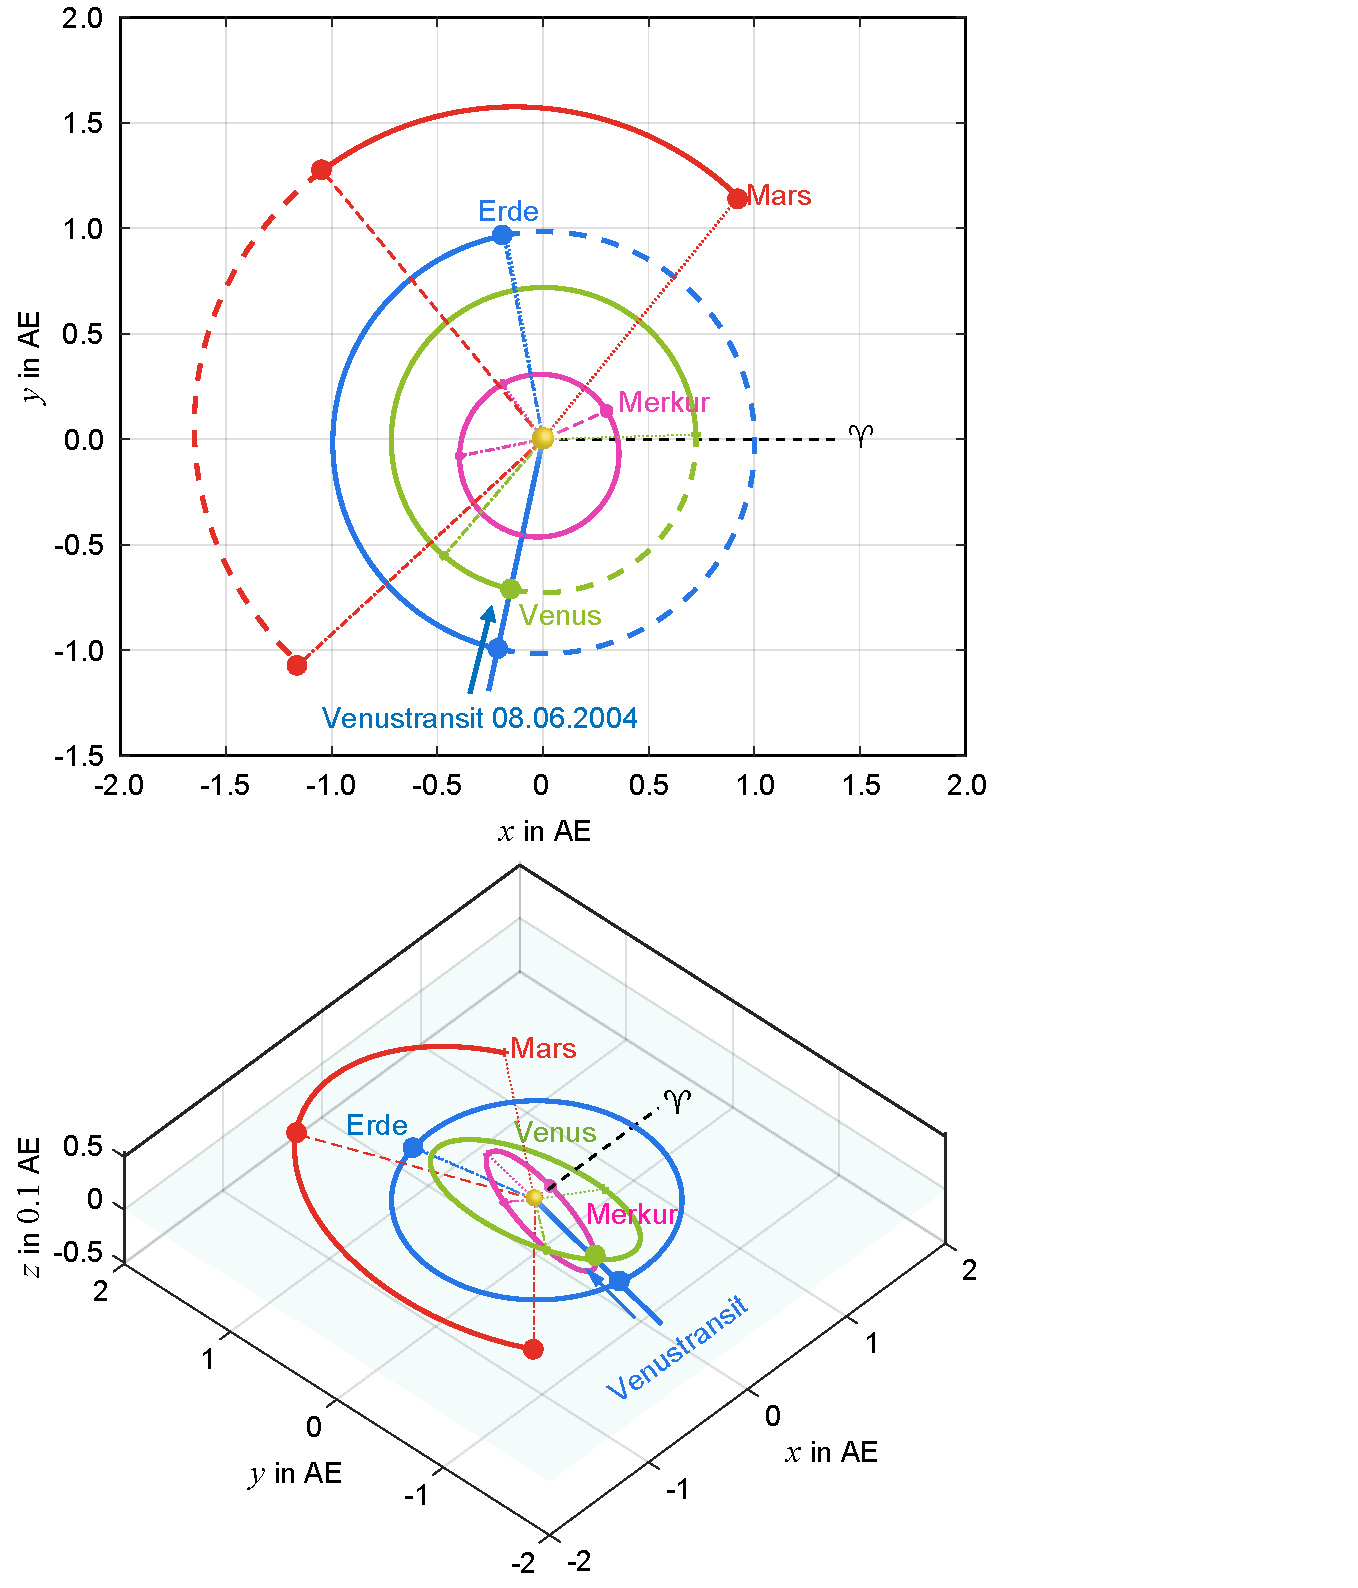
\includegraphics[width=\textwidth]{InnerePlaneten.pdf}\\%
\caption[Projektion der Bahnen der inneren Planeten auf die Ekliptik.]{Projektion der Bahnen der inneren Planeten auf die Ekliptik f�r das Jahr 2004 in Draufsicht (oben) und 3D-Darstellung (unten). Die Bahnen sind unterschiedlich f�r die Zeitr�ume 01.\,01.\,2004 bis 07.\,06.\,2004 (durchgezogen) und 08.\,06.\,2004 bis 31.\,12.\,2004 (gestrichelt) gezeichnet. F�r den 08.\,06.\,2004 erkennt man einen Venustransit\index{Venustransit}, das ist ein Durchgang der Venus vor der Sonnenscheibe, wie er von der Erde aus beobachtet werden konnte (dicke blaue durchgezogene Linie).}%
\label{abb:hm_proj_bahnen_innere_pl}%
\end{figure}

\begin{figure}%
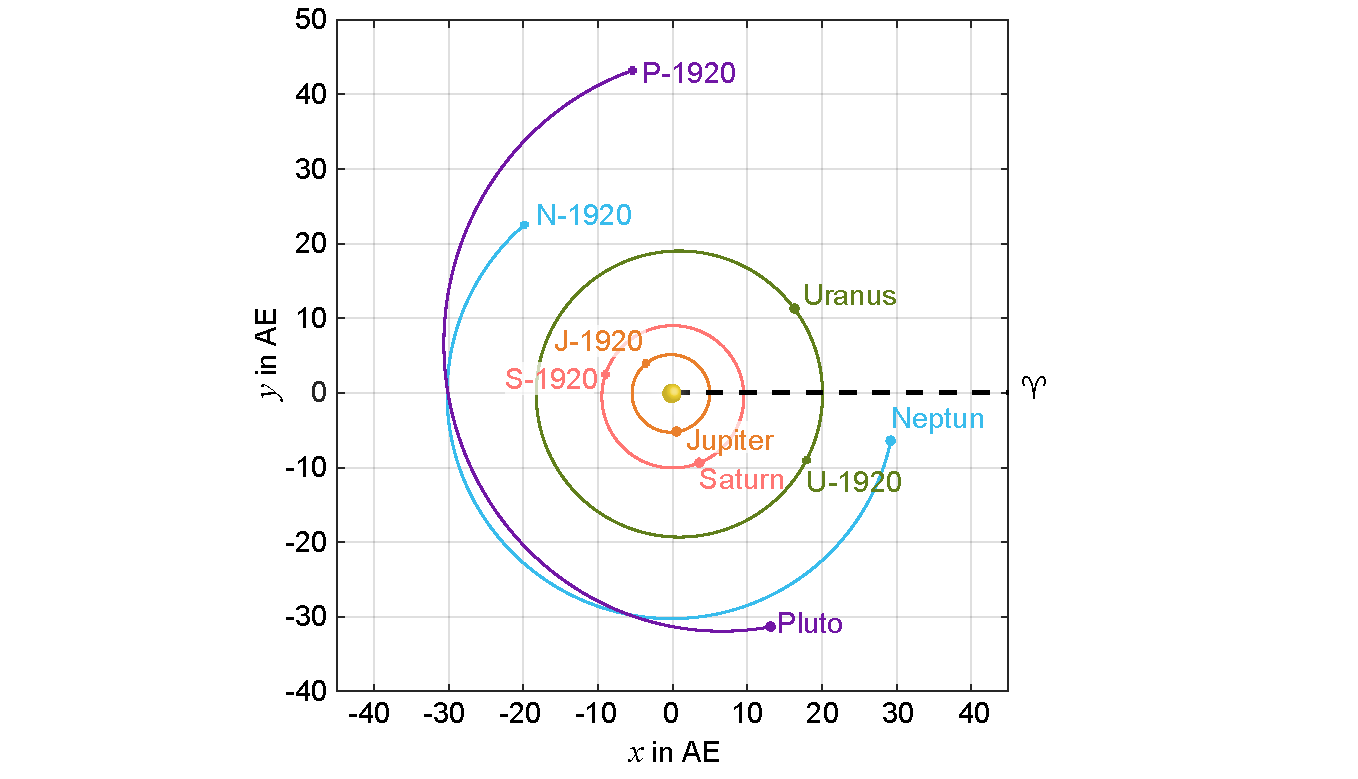
\includegraphics[width=\textwidth]{AeusserePlaneten.pdf}%
\caption{Bahnen der �u�eren Planeten im Zeitraum von 1920 bis 2020.}%
\label{abb:hm_bahnen_aussere_pl}%
\end{figure}

\subsubsection{N�herungsformel f�r die Berechnung der Bahnen von Planeten -- Reduktion auf die Ekliptik}\label{kap:reduktion_ekliptik}\index{Reduktion!auf die Ekliptik}
Bei Planeten ist im Gegensatz zu den sp�ter behandelten Kometen die Neigung der Bahn $i$ gegen die Ekliptik im Allgemeinen relativ klein.
Deshalb kann man eine N�herungsformel f�r die Berechnung der ekliptikalen Koordinaten aus den Bahnkoordinaten herleiten.
Die Herleitung dieser sogenannten Reduktionsformel\index{Reduktionsformel} ist in Beispiel \ref{bsp:herleitung_redformel_ekl} im Detail ausgef�hrt.
Man startet bei \figref{hm_planetenbahnen_rel_ekliptik} und benutzt die aus der sph�rischen Trigonometrie bekannte Beziehung (siehe auch die \onlineZ)
\begin{equation}
\tan(l-\Omega) = \cos\epsilon\tan(\upsilon+\omega)~. \label{eq:hm_reduktions_formel1}
\end{equation}

Die sogenannte Reduktion\index{Reduktion} $\mathcal{R}$ ist definiert als Differenz von ekliptikaler L�nge und wahrer Anomalie (abz�glich des konstanten Wertes $\varpi$ der L�nge des Perihels):
\begin{equation}
\mathcal{R} = l-(\upsilon+\varpi) \label{eq:hm_reduktions_formel2} ~.\\
\end{equation}

Wir geben hier das Resultat f�r $\mathcal{R}$ an und verweisen auf die detaillierte Rechnung in Bsp. \ref{bsp:herleitung_redformel_ekl}:
\begin{equation}
\mathcal{R} = -\tan^2\lk\frac{i}{2}\rk \sin\lek 2(M+\omega) \rek + \frac{1}{2} \lek \tan^2\lk\frac{i}{2}\rk\rek^2 \sin\lek 4(M+\omega) \rek - \ldots  ~.\label{eq:hm_reduktions_formel3}\\
\end{equation}
Aus \eqref{eq:hm_reduktions_formel2} folgt mit der Beziehung $l(t)\!\approx\!\upsilon(t) + \varpi + \mathcal{R}(t)\!\approx\!\mathcal{C}(t)+M(t)+\varpi + \mathcal{R}(t)$ die ekliptikale L�nge $l$ als Funktion der mittleren Anomalie $M$\glslink{mittlereanom}:
\begin{align}
\begin{split}
l(M) =& M + \varpi + 2e\sin M + \lek \frac{5}{4} e^2 - \tan^2\lk\frac{i}{2}\rk \cos(2\omega) \rek \sin(2M) \\ 
      &+ \lek -\tan^2\lk\frac{i}{2}\rk \sin(2\omega)\rek \cos(2M) + \ldots\,. 
\end{split} \label{eq:hm_reduktions_formel4} 
\end{align}
In �hnlicher Weise lassen sich Berechnungsformeln f�r die ekliptikale Breite $b$ und den Abstand $r$ gewinnen:
\begin{align}
b(M(t)) =& -ie\sin\omega + i\sin\omega\cos M + i\cos\omega\sin M \label{eq:hm_reduktions_formel5} \\ 
      & +ie\sin\omega\cos(2M) + ie\cos\omega\sin(2M) +\ldots\nonumber \\ \nonumber\\
r(M(t)) =& a\lk 1+\frac{e^2}{2} \rk - ae\cos M - a \frac{e^2}{2} \cos(2M) +\ldots\,. \label{eq:hm_reduktions_formel6} 
\end{align}
Diese elegante und einfach programmierbare Berechnung der ekliptikalen Koordinaten ist als N�herung f�r viele Anwendungsf�lle, insbesondere f�r Planeten mit geringer Bahnneigung, gut geeignet.
In den \textbf{�bungen} \ref{prob:hm_opposition_mars}, \ref{prob:hm_erdaufgang_von_mond} und \ref{prob:hm_erdaufgang_von_apollo} sind einige Anwendungsbeispiele f�r die Berechnung von Planeten- und Mondbahnen ausgef�hrt.\\
  
%BEISPIEL 6 %%%%%%%%%%%%%%%%%%%%%%%%%%%%%%%%%%%%%%%%%%%%%%%%%%%%%%%%%%%%%%%%%%%%%%%%%%%%%%%%%%
\begin{example}{Herleitung der Reduktionsformel auf die Ekliptik\index{Reduktion!auf die Ekliptik}}
\itshape Wir wollen die Reduktionsformel \eqref{eq:hm_reduktions_formel3} herleiten und starten dazu von \figref{hm_planetenbahnen_rel_ekliptik}.
Wir benutzen dabei vorteilhafterweise die Formeln, die wir bei der Herleitung der Mittelpunktsgleichung in \probref{hm_alternative_MPG} erhalten haben.\\
\upshape
In \figref{hm_planetenbahnen_rel_ekliptik} gilt im sph�rischen Dreieck PKE$_\text{P}$ nach der sph�rischen Trigonometrie
\begin{equation*}
\cos i = \frac{\tan \overline{\text{KE}}_\text{P}}{\tan \overline{\text{KP}}} = \frac{\tan(l-\Omega)}{\tan(\upsilon+\omega)} = \frac{\tan\Theta}{\tan u} \,,
\end{equation*}
worin $\upsilon$ wieder die wahre Anomalie ist und $l$ die ekliptikale L�nge, also
\begin{equation*}
\tan\Theta = \cos i \tan u \,.
\end{equation*}
Wir dr�cken nun $\cos i$ durch den Tangens des halben Winkels aus und erhalten
\begin{equation*}
\tan\Theta = \frac{1-\tan^2\lk\frac{i}{2}\rk}{1+\tan^2\lk\frac{i}{2}\rk} \tan u \equiv \frac{1-y}{1+y} \tan u \,.
\end{equation*}
Diese Gleichung haben wir in gleicher Struktur in \probref{hm_alternative_MPG} ausgewertet und sind dort auf die folgende Form gekommen:
\begin{align*}
\upsilon &= E + 2 \lk x\sin E + \frac{x^2}{2}\sin 2E + \frac{x^3}{3}\sin 3E + \ldots \rk ~.
\end{align*}
Hier ist $x\!=\!-y$, $\upsilon \!=\! 2 \Theta$ und $E\!=\!2u$ zu setzen, woraus folgt:
\begin{align*}
\Theta &= u- y\sin 2u + \frac{y^2}{2}\sin 4u - \frac{y^3}{3}\sin 6u + \ldots \,.
\end{align*}
Wir setzen jetzt wieder $\Theta\!=\!l-\Omega$ und $u\!=\!\upsilon+\omega$ und k�nnen schreiben:
\begin{align*}
l - (\Omega  + \omega) &= l - \varpi \\
&= \upsilon - y\sin\lk 2(\upsilon+\omega)\rk + \frac{y^2}{2}\sin\lk 4(\upsilon+\omega)\rk + \ldots ~.
\end{align*}
F�r die meisten Planeten ist $i\!<\!10\degree$, sodass $y\!=\!\tan^2(i/2)$ eine kleine Gr��e ist und wir Terme mit $y^2$ und h�her vernachl�ssigen k�nnen.
Wir setzen jetzt f�r $\upsilon$ die Mittelpunktsgleichung \eqref{eq:hm_mpglg_nu-M} mit $\upsilon\!=\! M + \mathcal{C} = M + 2e\sin M + \frac{5e^2}{4}\sin(2M) +  \ldots$ ein und erhalten
\begin{align*}
l & \approx \! \varpi + \underbrace{M + 2e\sin M + \frac{5e^2}{4}\sin(2M)}_{\upsilon = M + \mathcal{C}} \\ 
&- y\lek \sin(2(\upsilon)) \cos(2\omega) + \cos(2(\upsilon)) \sin(2\omega)\rek + \ldots ~.
\end{align*}
Wir k�nnen f�r kleine $e$ in den Winkelfunktionen $\upsilon \approx M$ setzen und erhalten schlie�lich
\begin{align}
\begin{split}
l &\approx \! \varpi + M + 2e\sin M + \lek \frac{5e^2}{4} - \tan^2\lk\frac{i}{2}\rk \cos(2\omega) \rek \sin(2M) \\
& - \lek \tan^2\lk\frac{i}{2}\rk \sin(2\omega) \rek \cos(2M) + \mathcal{O}\lk e^3,\tan^4\lk\frac{i}{2}\rk \rk\,,
\end{split} \label{eq:hm_reduktions_formel_Bsp}
\end{align}
was Gleichung \eqref{eq:hm_reduktions_formel4} entspricht.\\
Vergleicht man die Geometrie von \figref{hm_planetenbahnen_rel_ekliptik}, f�r die wir die Reduktionsformel abgeleitet haben, mit der Geometrie von \figref{hm_wahre_sonne_geoz}, erkennt man, dass wir die Reduktionsformel auch in diesem Fall, der sogenannten Reduktion auf den �quator\index{Reduktion!auf den �quator}, anwenden k�nnen.
Wir m�ssen dann nur folgende Substitution vornehmen: $l\!\rightarrow\!\lambda $ und $\upsilon + \varpi\!\rightarrow\!\alpha$. \\

\label{bsp:herleitung_redformel_ekl}
\end{example}
%BEISPIEL %%%%%%%%%%%%%%%%%%%%%%%%%%%%%%%%%%%%%%%%%%%%%%%%%%%%%%%%%%%%%%%%%%%%%%%%%%%%%%%%%%

\subsubsection{Venustransit}\index{Venustransit} \label{kap:hm_veustransit}

In \figref{hm_proj_bahnen_innere_pl} haben wir gesehen, dass am 08.\,06.\,2004 Erde, Venus und Sonne in einer Linie \anf{lagen}.
Unter Ber�cksichtigung des scheinbaren Durchmessers der Sonne von \ca $30'$ ergibt unsere Rechnung, dass zumindest prinzipiell (abh�ngig von der genauen topozentrischen Position) ein Beobachter auf der Erde einen Venustransit beobachten kann, \dh er kann sehen, wie sich die Venus vor die Sonne bewegt
(Tab.~\ref{tab:hm_venustransit}).
Tats�chlich war f�r viele Beobachter in Mitteleuropa das Wettergl�ck auf ihrer Seite und der Transit sehr sch�n zu beobachten (\figref{hm_venustransit}).
Venustransits geh�ren zu den seltensten der exakt vorhersagbaren astronomischen Ereignisse.
Kein im Jahre 2004 lebender Mensch hatte zuvor einen solchen Transit beobachten k�nnen, weil im gesamten vergangenen 20.\ Jahrhundert kein einziger stattfand.
Der n�chste Transit wird erst wieder im Jahre 2117 zu verfolgen sein.
Seit dem Aufkommen des Teleskops konnten �berhaupt nur sieben Venustransits von Menschen beobachtet werden (1639, 1761, 1769, 1874, 1882, 2004, 2012). 

\begin{figure}%
\includegraphics[width=\textwidth]{VenustransitKombi.pdf}%
\caption[Venustransit 2004.]{\fa Venustransit 2004 (Private Aufnahme um 06:40 UT in 48.8�N/10.7�O) und \fb Berechnung mit den \mscr en \mlhmref{VenusTransit01.m} und \mlhmref{VenusTransit02.m}.}%
\label{abb:hm_venustransit}%
\end{figure}

Unserer Rechnungen mit den \mscr en \mlhmref{VenusTransit01.m} \bzw \mlhmref{VenusTransit02.m} ergeben relativ genaue Ergebnisse, weichen jedoch geringf�gig von den Daten des \textit{\gls{jplhm}~(JPL)}\index{Jet Propulsion Lab (JPL)} \cite{JPL2020} ab.%
\footnote{Mit unserem \mscr{} findet man noch mit guter Genauigkeit einen weiteren Transit der Venus f�r den 06.\,06.\,2012.} Dies erkl�rt sich, wenn man bedenkt, dass wir
\begin{itemize}
	\item reine Keplerbahnen angenommen haben, \dh den Einfluss der anderen Planeten und vor allem des Mondes auf die Erdbahn vernachl�ssigt haben,
	\item die Pr�zession der Erdachse in unserer Rechnung nicht ber�cksichtigt haben.
\end{itemize}
Die Ber�cksichtigung dieser Effekte ist Gegenstand der St�rungstheorie, deren Grundidee wir in \kap{stoerungsrechnung} vorstellen wollen. 

\begin{table}%
\caption[Koordinaten von Erde, Venus und Sonne am 08.06.2004 um 08:00 und 12:00 UT.]{Koordinaten von Erde, Venus und Sonne am 08.06.2004 um 08:00 und 12:00 UT. Die Rektaszension $\alpha$ ist wie �blich in \text{hh}$^\text{h} \text{mm}^\text{m} \text{ss}^\text{s}$ angegeben.}
\begin{adjustbox}{width=\textwidth,totalheight=\textheight,keepaspectratio}
\begin{tabular}{l|c|cc|cc|cc}
\hline\noalign{\smallskip}
 - & UT & \multicolumn{2}{c|}{Sonne} & \multicolumn{2}{c|}{Venus} & \multicolumn{2}{c}{Erde} \\
\noalign{\smallskip}\svhline\noalign{\smallskip}
Heliozentrisch & & & & $l$ & $b$ & $l$ & $b$ \\
\noalign{\smallskip}\svhline\noalign{\smallskip}
\multirow{2}{*}{JPL \cite{JPL2020}} & 08:00 &  &  & $257.7883\degree$ & $-0.0665\degree$ & $257.8015\degree$ & $0.0007\degree$ \\
                                    & 12:00 &  &  & $258.0527\degree$ & $-0.0822\degree$ & $257.9609\degree$ & $0.0007\degree$\\
\hline\noalign{\smallskip}		
\multirow{2}{*}{\mlhmref{InnerePlaneten.m}} 
																	& 08:00 &  &  & $257.7885\degree$ & $-0.0662\degree$ & $257.8015\degree$ & $-0.0005\degree$ \\
																	& 12:00 &  &  & $258.0529\degree$ & $-0.0813\degree$ & $257.9837\degree$ & $-0.0005\degree$ \\
\noalign{\smallskip}\svhline\noalign{\smallskip}
Geozentrisch & & $\lambda$ & $\beta$ & $\lambda$ & $\beta$ &  &  \\
\noalign{\smallskip}\svhline\noalign{\smallskip}
\multirow{2}{*}{JPL \cite{JPL2020}} & 08:00 & $77.8605\degree$ & $-0.0002\degree$ & $77.9079\degree$ & $-0.1691\degree$ &  &  \\
                                    & 12:00 & $78.0199\degree$ & $-0.0002\degree$ & $77.8031\degree$ & $-0.2086\degree$ &  &  \\
\hline\noalign{\smallskip}		
\multirow{2}{*}{\mlhmref{InnerePlaneten.m}} 
                                  & 08:00 & $77.8243\degree$ & $0.0005\degree$ & $77.9143\degree$ & $-0.1630\degree$ &  &  \\
																	& 12:00 & $77.9837\degree$ & $0.0005\degree$ & $77.8097\degree$ & $-0.2025\degree$ &  &   \\		
\noalign{\smallskip}\svhline\noalign{\smallskip}
�quatorial & & $\alpha$ & $\delta$ & $\alpha$ & $\delta$ &  &  \\
\noalign{\smallskip}\svhline\noalign{\smallskip}
JPL \cite{JPL2020} 
	& 08:00 & $05^\text{h}06^\text{m}51^\text{s}$ & $22\degree52'46''$ & $05^\text{h}07^\text{m}16^\text{s}$ & $22\degree42'55''$ &  &  \\
	& 12:00 & $05^\text{h}07^\text{m}41^\text{s}$ & $22\degree53'38''$ & $05^\text{h}06^\text{m}50^\text{s}$ & $22\degree40'00''$ &  &  \\
\hline\noalign{\smallskip}		
\mlhmref{InnerePlaneten.m}
	& 08:00 & $05^\text{h}07^\text{m}04^\text{s}$ & $22\degree52'54''$ & $05^\text{h}07^\text{m}31^\text{s}$ & $22\degree43'37''$ &  &  \\
	& 12:00 & $05^\text{h}07^\text{m}45^\text{s}$ & $22\degree53'46''$ & $05^\text{h}07^\text{m}05^\text{s}$ & $22\degree40'42''$ &  &  \\
\noalign{\smallskip}\hline\noalign{\smallskip}
\end{tabular}
\end{adjustbox}
\label{tab:hm_venustransit}
\end{table}

\begin{figure}
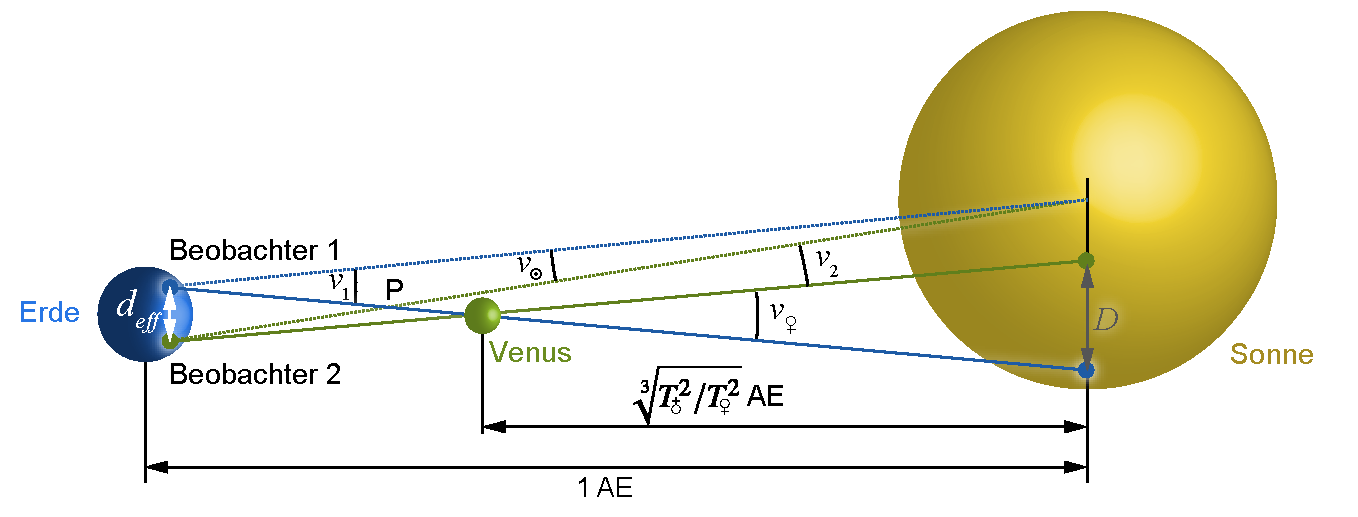
\includegraphics[width=\textwidth]{VenusParallax_exakt.pdf}%
\caption[Messung der Venus-Parallaxe f�r zwei Beobachter auf der Erde.]{Messung der Venus-Parallaxe f�r zwei Beobachter auf der Erde (allgemeiner Fall, nach \cite{Backhaus2020}).}%
\label{abb:hm_VenusParallax}%
\end{figure}

Venustransits sind auch wissenschaftshistorisch sehr interessant.
Die gleichzeitige Beobachtung des Transits von verschiedenen Orten der Erde aus erlaubte erstmalig die genaue Bestimmung des Abstandes zwischen Sonne und Erde, \dh der Astronomischen Einheit\index{Astronomischen Einheit} (AE)\glslink{ae}.
Hierbei nutzte man aus, dass die Position der Venus relativ zur Sonnenscheibe im Prinzip gut messbar ist (\figref{hm_VenusParallax}).
Deshalb machte Halley\indexp{Halley, Edmund}\footnote{Edmund Halley (1656--1742) war k�niglicher Astronom und Leiter der Sternwarte in Greenwich, Mathematiker, Kartograph, und Meteorologe. Neben seinen Berechnungen von Kometenbahnen erforschte Halley auch den Erdmagnetismus, den Monsun, die Eigenbewegung von Sternen und berechnete die \index{H�henformel!barometrische} \glslink{baroHoeheHm}{barometrische H�henformel}.} bereits 1716 den Vorschlag, beim (f�r ihn) n�chsten Venustransit 1761 (den er nicht mehr erlebte) von verschiedenen Orten der Erde (effektiver Abstand $d_\text{eff}$) aus die Parallaxe $\nu_\text{1,2}$ der Venus auf der Sonnenscheibe gleichzeitig zu vermessen (\figref{hm_VenusParallax}).
Um daraus die Sonnenentfernung so genau wie m�glich bestimmen zu k�nnen, muss die Entfernung Sonne-Venus auf die Entfernung Erde-Sonne nach dem 3.~Keplerschen Gesetz $a_\text{\earth}\!=\!a_\text{\venus}\,\sqrt[3]{T_\text{\earth}^2/T_\text{\venus}^2} $ hochgerechnet werden, woraus sich dann mit $\Delta\nu = \nu_\text{1} -\nu_\text{2}$ die astronomische Einheit bestimmen l�sst zu
\begin{equation}
1 \text{AE} = a_\text{\earth} =\frac{d_\text{eff}}{\lk \frac{a_\text{\earth}}{a_\text{\venus}} - 1 \rk \Delta\nu}\,.\label{eq:hm_Venus_AE_Messung}
\end{equation}
Die Entfernung zwischen Erde und Sonne ist die Grundlage f�r die Bestimmung der Gr��e des Sonnensystems und damit auch f�r die Messung der astrophysikalischen Eigenschaften (wie Massen, Dichten) von Planeten und Sternen.
Bis zum 17. Jahrhundert existierten nur vage Vorstellungen �ber die Gr��enordnung dieser Entfernung und die Bestimmung dieser Gr��e galt f�r viele Jahrhunderte als eines der Hauptprobleme der Astronomie.
Deshalb war es auch nicht ganz verwunderlich, dass 1761 (und auch 1769) auf Basis von Halleys Vorschlag mit viel Geld eine ganze Reihe von Expeditionen �ber Monate in entlegenste Gebiete geschickt wurden -- wobei einige dann am Tag des Venustransits einen bew�lkten Himmel oder defekte Instrumente vorfanden.\footnote{Eine sehr sch�ne und spannende Darstellung dieses ersten gro�en internationalen Wissenschaftsabenteuers findet man in \cite{Wolf2017}.
Eine ebenfalls lesenswerte und kurz zusammengefasste Geschichte der Bestimmung der AE findet sich in \cite{Hudson2004}.} Heute in Zeiten des Internets ist das nat�rlich viel einfacher realisierbar \cite{Backhaus2014}.
Wir empfehlen dazu Beispiel \ref{bsp:venustransit} und \probref{hm_venus_2004_2012} durchzuarbeiten, in denen wir konkret die Vorgehensweise zur Bestimmung der Astronomischen Einheit nachvollziehen.

%BEISPIEL 7 %%%%%%%%%%%%%%%%%%%%%%%%%%%%%%%%%%%%%%%%%%%%%%%%%%%%%%%%%%%%%%%%%%%%%%%%%%%%%%%%%%

\begin{example}{Venustransit und Bestimmung der AE}
\begin{enumerate}[(a)]
  \item Wir wollen zeigen, wie aus der gleichzeitigen fotografischen Beobachtung des Venustransits an zwei verschiedenen Positionen auf der Erde mit bekannten Koordinaten die Astronomische Einheit bestimmt werden kann (siehe \figref{hm_VenusTransit2012}).
    Wir wollen dazu Daten einer solchen Beobachtung, die man im Internet \zb unter \cite{Venustransit2012} finden kann, benutzen.\\
\begin{center}
	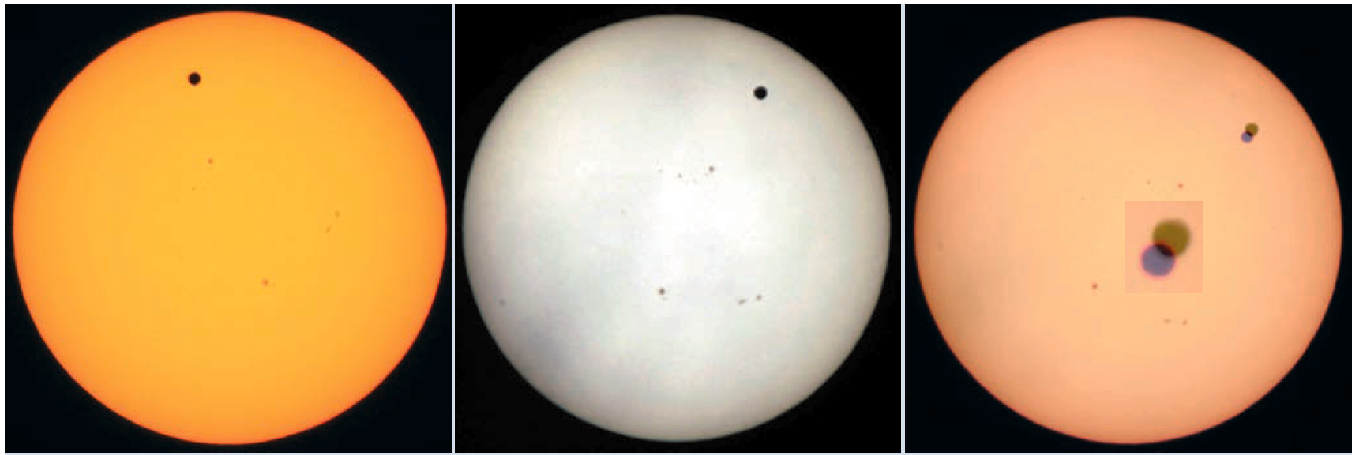
\includegraphics[width=0.9\textwidth]{VenusTransit2012.pdf} 
\captionof{figure}[Venustransit 2012.]{Venustransit 2012. Zeitgleiche Aufnahmen des Transits aus Troms� (links) und Canberra (Mitte) \cite{Venustransit2012}. Im rechten Bild sind die beiden Bilder mit der gleichen Ausrichtung der Sonnenachse �berlagert. (Man benutzt dazu z.B. die Position der Sonnenflecken). Im rechten Bild ist in der Mitte zur Verdeutlichung eine Vergr��erung des Winkelunterschiedes der in den beiden Standorten sich unterscheidenden Venusprojektionen zu sehen.}\label{abb:hm_VenusTransit2012}
\end{center}

Man kann aus dem Bild durch Ausmessen den Winkelunterschied f�r die beiden Projektionen zu $\Delta\nu \approx 0.021 \, b_\text{w\astrosun}$ bestimmen, worin $b_\text{w\astrosun} = 0.5317\degree$ der Bildwinkel der Sonne ist, unter dem sie von der Erde aus erscheint.
        Den effektiven Abstand zwischen Troms� und Canberra berechnet man zu $d_\text{eff} = 11415 \:\text{km}$ (\probref{hm_venus_2004_2012}).
        Aus \eqref{eq:hm_Venus_AE_Messung} ergibt sich dann mit den Werten $	T_\text{\venus} = 224.701 \:\text{d}, T_\text{\earth} = 365.256 \:\text{d}$:
\begin{align*}
	\gamma \!&= \!\frac{a_\text{\earth}}{a_\text{\venus}}=\sqrt[3]{\frac{T_\text{\earth}^2}{T_\text{\venus}^2}}= 1.382~~\text{und daraus}\\ 
\rightarrow a_\text{\earth} \!&=\:\!152.6\: \text{Mio km}
\end{align*}

Dieser Wert stimmt relativ gut mit dem exakten Wert �berein.
Ungenauigkeiten resultieren vor allem aus der Bestimmung von $\Delta\nu$ aus den Fotografien.
	\item Man kann die Bestimmung der Astronomischen Einheit auch durch einen einzigen Beobachter an einem festen Ort der Erde realisieren.
          Bei der zeitlichen Verfolgung des Venustransits nutzt man die durch die Erdrotation entstehende Parallaxe aus.
          Man muss dann die sogenannten Kontaktzeiten bestimmen, z.\,B. die Zeit $T_\text{II}$ bzw. $T_\text{III}$, wenn der Rand der Venusprojektion den Rand der \anf{Sonnenscheibe} von innen ber�hrt.
          Alternativ bestimmt man die Transitzeit $T_\text{TR}$, die sich die Venusprojektion vom Ort des Beobachters betrachtet auf der Sonnenscheibe befindet.
          Diese Transitzeit betr�gt einige Stunden und muss sehr genau ermittelt werden, was hohe Anforderungen an die Messung stellt.
          Wir wollen die Genauigkeit der Kontaktzeitmethode\index{Kontaktzeitmethode} mit der Genauigkeit der Parallaxenmethode\index{Parallaxe} an zwei Beobachtungsorten vergleichen \cite{Rempel2019} und nehmen dabei zun�chst f�r eine erste Absch�tzung vereinfachend an, dass die Planeten Erde und Venus sich auf kreisf�rmigen Bahnen in der Ekliptikebene um die Sonne bewegen.\\
	Wir betrachten dazu in \figref{hm_VenusTransitd}
        den Fall (a).
        F�r die L�nge der Projektion auf der Sonne gilt
	\begin{align*}
		\frac{\D s_\text{\venus}-\D s_\text{\earth}}{a_\text{\earth}-a_\text{\venus}}&=\frac{\D P_\text{B} - \D s_\text{\earth}}{a_\text{\earth}}~.
		\end{align*}
		Mit den Beziehungen f�r die Winkelgeschwindigkeiten $\D s_i\!=\!\omega_i a_i \D t$, $\D P_\text{B}\!=\!\Omega_\text{B} a_\text{\earth} \D t$ und $\gamma\!=\! a_\text{\earth}/a_\text{\venus}$ erhalten wir
	\begin{align*}
\Omega_\text{B} = \frac{1}{a_\text{\earth}} \frac{\D P_\text{B}}{\D t}= \frac{\omega_\text{\venus} - \omega_\text{\earth} }{\gamma-1} ~.
	\end{align*}
$\Omega_\text{B}$ ist die Winkelgeschwindigkeit des Projektionspunktes auf der Sonnenscheibe.
Wir nehmen weiter an, dass der Venustransit durch den Sonnenmittelpunkt verlaufe.
Dann ist die maximal m�gliche Transitzeit gegeben durch
\begin{equation*}
T_\text{TR,max} = \frac{b_\text{w\astrosun}}{\Omega_\text{B}}=28500 \:\text{s} \approx \:7\:\text{h}\:54\:\text{min} \,.
\end{equation*}	
Wie wir in \figref{hm_venustransit} sehen, erfolgt der Transit aber entlang einer Sehne mit der relativen L�nge $l_\text{S\astrosun}$.
Wir k�nnen diese L�nge wiederum gut im Verh�ltnis zu $b_\text{w\astrosun}$ aus den fotografischen Aufnahmen zu $\approx 0.78$ bestimmen, woraus sich eine Transitzeit $T_\text{TR,B}$ in guter N�herung ergibt zu
\begin{equation*}
T_\text{TR}= \frac{l_\text{S\astrosun} \, b_\text{w\astrosun}}{\Omega_\text{B}} = 22230\:\text{s} \approx \:6\:\text{h}\:11\:\text{min} \,.
\end{equation*}	
Das entspr�che der Transitzeit f�r einen Beobachter im Erdmittelpunkt.

\begin{center}
	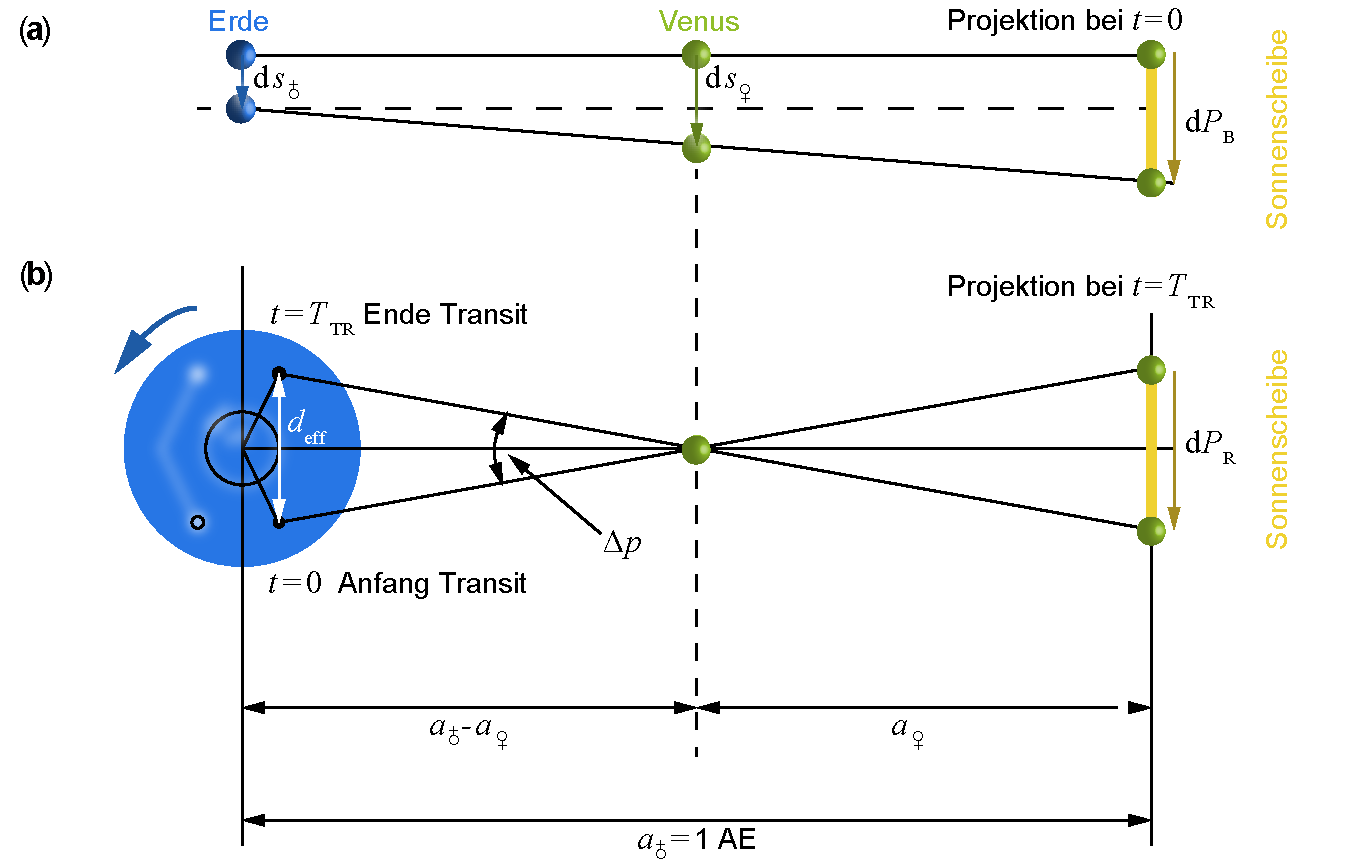
\includegraphics[width=\textwidth]{Venustransitd.pdf}
\captionof{figure}[Schematische Darstellung der Kontaktzeitmethode.]{Schematische Darstellung der Kontaktzeitmethode.
Betrachtung der Venus-Projektionen \fa ohne \fb mit Erdrotation.}\label{abb:hm_VenusTransitd}
\end{center}

Jetzt kommt noch die Erdrotation ins Spiel, die uns wiederum eine Parallaxe liefert.
Anstelle der r�umlichen Differenz zweier Beobachter zum gleichen Zeitpunkt m�ssen wir jetzt die r�umliche Differenz eines ortsfesten Beobachters zu zwei Zeiten betrachten.
Aus \figref{hm_VenusTransitd}b erkennen wir, dass die Erdrotation eine zus�tzliche Winkelgeschwindigkeit $\Omega_\text{B}$ f�r die Projektion bewirkt, die sich �ber 
\begin{equation*}
\frac{d_\text{eff}}{a_\text{\earth} - a_\text{\venus}} = \frac{\D P_\text{R}}{a_\text{\venus}}
\end{equation*}	
berechnet zu 
\begin{equation*}
\Omega_\text{R} = \frac{1}{a_\text{\earth}} \frac{\D P_\text{R}}{\D t} = \frac{d_\text{eff}}{T_\text{TR} a_\text{\earth} \lk \gamma -1 \rk}  \,.
\end{equation*}	
Die reale von einem Beobachter auf der Erdoberfl�che gemessene Transitzeit ist daher gegeben durch
\begin{align*}
T_\text{TR,B} &= \frac{b_\text{w\astrosun} \, l_\text{S\astrosun}}{\Omega_\text{B} + \Omega_\text{R}}
= \frac{b_\text{w\astrosun} \, l_\text{S\astrosun}}{\Omega_\text{B} + \lek d_\text{eff} / \lk T_\text{TR,B} \:  a_\text{\earth} (\gamma -1) \rk \rek} \; .
\end{align*}
Auch hier haben wir wieder eine Bestimmungsgleichung f�r die Astronomische Einheit in einer Abh�ngigkeit zu bekannten terrestrischen Distanzen ($d_\text{eff}$) und einer Zeitmessung erhalten:
\begin{equation}
1 \text{AE}\!=\!a_\text{\earth} \!=\!\frac{d_\text{eff}}{(\gamma - 1 )\lk b_\text{w\astrosun} \, l_\text{S\astrosun} - \Omega_\text{B} \, T_\text{TR,B} \rk}  \,.\label{eq:hm_Venus_AE_KontaktMessung}
\end{equation}
Die Gr��en $b_\text{w\astrosun}$, $\Omega_S$ und $\gamma$ sind bekannt.
$l_\text{S\astrosun}$ und $T_\text{TR,B}$ werden gemessen.
Damit man eine ausreichende Genauigkeit bei der Bestimmung der Astronomische Einheit bekommt, muss man die Sehnenl�nge $l_\text{S\astrosun}$ und vor allem $T_\text{TR,B}$ sehr genau bestimmen, da der Nenner in \eqref{eq:hm_Venus_AE_KontaktMessung} gegen Null geht.
Das ist die eigentliche Herausforderung dieser Methode.
In \probref{hm_venus_2004_2012} berechnen wir f�r Messwerte von 2004 nach dieser einfachen Methode den Wert der AE.
Zudem verfeinern wir die Methode, indem wir die Annahmen konzentrischer und koplanarer Kreisbahnen fallen lassen. \\

\end{enumerate}
\label{bsp:venustransit}
\end{example}
%BEISPIEL %%%%%%%%%%%%%%%%%%%%%%%%%%%%%%%%%%%%%%%%%%%%%%%%%%%%%%%%%%%%%%%%%%%%%%%%%%%%%%%%%%

Analog zu Venustransits gibt es auch Merkurtransits.
Diese sind auf Grund der k�rzeren Umlaufperiode des Merkurs naturgem�� h�ufiger.
Sie erlauben ebenfalls die Bestimmung der Astronomischen Einheit, allerdings mit geringerer Pr�zision.
Die letzten Merkurtransits wurden in Europa im Mai 2016 und im November 2019 beobachtet, und den n�chsten wird es schon wieder 2032 geben.
Das wirft die Frage auf, ob es auch gemeinsame Transits von Merkur und Venus vor der Sonne geben kann.
Tats�chlich gibt es solche und der n�chste wird \anf{schon} am 26.\,07.\,69163 beobachtbar sein \cite{Meeus2004}.
F�r solche gro�en Zeitabst�nde reicht die Genauigkeit unserer Rechnung allerdings nicht aus.
Die f�r den 22.\,11.\,2065 vorhergesagte Bedeckung des Planeten Jupiter durch die Venus ist hingegen mit unserer einfachen Keplerrechnung (\probref{hm_jupiterbedeckung_venus}, \mscr{} \mlhmref{InnerePlaneten.m}) zumindest prinzipiell vorhersagbar.
F�r die Bestimmung der genauen Beobachtungszeiten und -koordinaten reicht das aber nicht mehr aus.
Dazu braucht man genauere Ephemeriden.
Wir werden uns deswegen jetzt mit den grundlegenden Prinzipien der St�rungsrechnung besch�ftigen, mit welcher man genauere Planetenbahnen auch �ber l�ngere Zeiten berechnen kann.
Zun�chst aber wollen wir uns noch mit dem Mehrk�rperproblem etwas genauer besch�ftigen, das wir bereits in der Physik der Bewegung (Band I, Kapitel 1) vorgestellt und f�r Spezialf�lle (eingeschr�nktes Dreik�rperproblem) behandelt hatten.

\subsection{Das Mehrk�rperproblem}\index{Mehrk�rperproblem} \label{kap:mehrkoerperproblem}

So einfach und elegant die Bahnberechnung auf Basis des Zweik�rperproblems\index{Zweik�rperproblem} auch ist, die Nichtber�cksichtigung von St�rungen der einfachen Keplerbahn durch andere Himmelsk�rper stellt eine echte Begrenzung f�r die Berechnung vieler realer Situationen in der Astronomie dar.
Der logische Schritt w�re daher, die Bewegungsgleichung \eqref{eq:hm_beschl_zk} auf $N$ K�rper (\figref{hm_Nkp} als Beispiel f�r $N\!=\!3$) zu erweitern.
Wir starten daher mit dem allgemeinen Ansatz
\begin{equation}
\vec{F}_i = m_i\,\ddot{\vec{r}}_i= -\sum_{j=1,j\neq i}^N \frac{G \, m_i m_j}{\left|\vec{r}_j - \vec{r}_i\right|^3}\cdot (\vec{r}_j - \vec{r}_i) \ \  ~~\text{f�r}~i=1,\ldots,N.\\
\label{eq:hm_beschl_N_koerper}\
\end{equation}

\begin{figure}
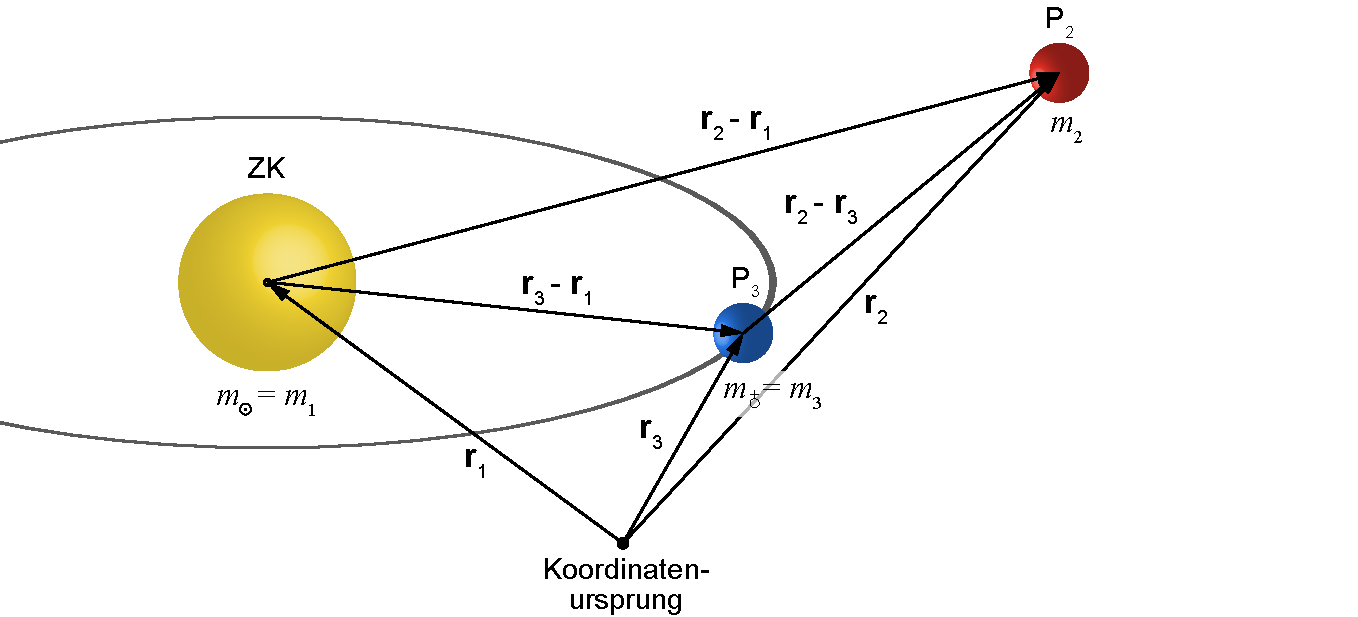
\includegraphics[width=\textwidth]{NKP.pdf}%
\caption[Geometrie eines Mehrk�rperproblems.]{Geometrie eines Mehrk�rperproblems am Beispiel der St�rung der Erdbahn durch einen weiteren �u�eren Planeten. ZK = Zentralk�rper ist in den folgenden Betrachtungen die Sonne, $\text{P}_3$ die Erde und $\text{P}_2$ ein �u�erer Planet oder der Erdmond.}
\label{abb:hm_Nkp}%
\end{figure}

Wie schon in Band I gezeigt, ist schon das Dreik�rperproblem ($N=3$) bis auf Spezialf�lle nicht mehr geschlossen analytisch l�sbar.
Es k�nnen daher auch keine geschlossenen Bewegungsgleichungen wie die Kepler-Gleichung\index{Kepler-Gleichung} f�r ein vermeintlich einfaches System, wie z.\,B. Sonne, Mond und Erde mehr angegeben werden. Es gibt aber f�r bestimmte Spezialf�lle L�sungen (siehe Band I), die physikalisch interessante und auch f�r die Praxis (\zb die Raumfahrt) relevante Schlussfolgerungen erlauben. 

\subsubsection{Ans�tze zur Behandlung des Mehrk�rperproblems}\label{kap:stoerungsrechnung}

F�r das \textit{allgemeine} Mehrk�rperproblem ohne Einschr�nkungen gibt es nun drei grunds�tzliche Ans�tze, mit denen man das (nichtlineare) System aus $3N$ Differentialgleichungen zweiter Ordnung basierend auf \eqref{eq:hm_beschl_N_koerper} behandeln kann: 
\begin{itemize}
	\item eine \emph{allgemeine St�rungstheorie}, die auf \emph{analytische Reihenentwicklungen} f�hrt,
	\item eine \emph{numerische Integration} und 
	\item \emph{spezielle St�rungstheorien}, die die numerische Integration vorbereiten.
\end{itemize}

Jede dieser Methoden hat ihre spezifischen Einsatzbereiche.
Die allgemeine St�rungstheorie mit ihren analytischen Reihenentwicklungen wird meist in der Planetentheorie benutzt, w�hrend die numerische Integration \zb bei der Berechnung von Kometen- und Asteroidenbahnen und auch in der Raumfahrt eingesetzt wird.
Wir stellen im Folgenden nur die Grundz�ge der beiden ersten Methoden dar. 
%Mit einigen speziellen St�rungsrechnungen werden wir uns im Kap. Astrodynamik (Kap. \ref{chap:adyn}) besch�ftigen. 
F�r eine ausf�hrliche Behandlung empfehlen wir als weiterf�hrende Literatur \ua die Darstellungen in \cite{Fitzpatrick2022, Walter2018, Guthmann2000, Brouwer1961, Murray2008}.\footnote{Eine sehr sch�ne und kompakte Darstellung der Effekte einer st�renden Kraft auf die Keplerbahn findet man in \cite{Burns1976}. In dieser Darstellung werden die Effekte �ber die Wirkung der St�rungskraft auf den Drehimpuls des ZKP beschrieben. Wir empfehlen diese Darstellung als gute physikalische Einf�hrung in die Methode der St�rungsrechnungen.} 

\subsubsection{Grundidee der allgemeinen St�rungsrechnung (analytische Reihenentwicklungen)}\index{Reihenentwicklung}\index{St�rungsrechnung}  \label{kap:Reihenentwicklung}

Wir starten von den Annahmen, dass 
\begin{itemize}
	\item die St�rungen relativ klein sind,
	\item die Massen der beteiligten Himmelsk�rper relativ weit voneinander entfernt sind und
	\item die Bahnen der Himmelsk�rper kleine Exzentrizit�ten haben und hinreichend stabil sind.
\end{itemize}
Letztere Annahme werden wir in den sp�teren Kapiteln \ref{kap:Periheldrehung} und \ref{kap:hm_langezeiten} noch etwas genauer betrachten.
Unter diesen Annahmen kann man die Bahnen als �berlagerung ungest�rter, sogenannter mittlerer Kepler-Ellipsen und kleiner periodischer St�rungen, sogenannter St�rterme, darstellen.
Wir hatten ja schon im vorhergehenden Kapitel gesehen, dass sich die ekliptikalen Koordinaten $l(t)$, $b(t)$, $r(t)$ als Funktion der Zeit (bzw. der mittleren Anomalie) in einer Reihenentwicklung angeben lassen (siehe Gleichungen \eqref{eq:hm_reduktions_formel4}--\eqref{eq:hm_reduktions_formel6}).
Die St�rungen durch den anderen Planeten ergeben nun zus�tzliche Terme in dieser Reihenentwicklung, welche als Argument die mittlere Anomalie des \bzw der \anf{st�renden} Himmelsk�rper und die des gest�rten Planeten, dessen Bahn wir berechnen wollen, enthalten.\footnote{Die mittleren Anomalien aller Planeten sind in Tabelle \ref{tab:hm_bahnparameter} angegeben.
Die Betrachtungen, die wir im Folgenden f�r den Fall $N\!=\!3$ anstellen, lassen sich ohne weiteres auf allgemeine F�lle $N>3$ �bertragen.}

\subparagraph{\textbf{Die St�rungsfunktion am Beispiel des Dreik�rperproblems }}\index{Dreik�rperproblem}\index{St�rungsfunktion} \label{kap:stoerungsfunktion} 
 
Ein relativ einfacher und instruktiver Fall ist das koplanare Dreik�rperproblem (siehe Kapitel 1.2.3.5 im Band I). Selbst dieses Problem erfordert schon eine anspruchsvolle mathematische Behandlung und l�sst erahnen, welche mathematische technische Komplexit�t hinter der St�rungsrechnung liegt. 
Wir verweisen hier auf die Spezialliteratur und empfehlen insbesondere \cite{Fitzpatrick2022} und \cite{Murray2008}.\\
%Wir skizzieren hier nur die generelle Vorgehensweise und verweisen ansonsten auf die Spezialliteratur cite{Fitzpatrick2022, Murray2008}.\\

\subparagraph{\textbf{Standard-St�rungsrechnungen und Tabellen}} \label{kap:stoerungstabellen}

Die berechneten St�rungsterme, wie im vorhergehenden Teil skizziert,  werden \ia in umfangreichen Tabellen angegeben (\ua \cite{Montenbruck1999, Murray2008}).
Es ist eine der gro�en Leistungen vieler Generationen von Astronomen, Mathematikern und Physikern, die mit diesen analytischen Reihenentwicklungen -- die oft hunderte von Termen umfassen -- hochgenaue Berechnungen f�r die Planeten ermittelt und damit auch ganz wesentlich zum Erkenntnisfortschritt in der Physik und Astrophysik beigetragen haben (siehe \kapitel{Periheldrehung}).\footnote{Man mache sich klar, dass diese Rechnungen bis in die Mitte des 20.\ Jahrhunderts ohne elektronische Computer gemacht wurden. Man sprach auch davon, dass Astronomie im 18.\ und 19.\ Jahrhundert \iw Rechnen war, wof�r sehr oft Frauen als sogenannte \anf{Computer} eingesetzt wurden. Viele dieser Frauen leisteten sp�ter wichtige eigenst�ndige Beitr�ge in der Astronomie und Astrophysik.}
Dar�ber hinaus gab es aber auch ganz praktische und �konomisch hochrelevante Beweggr�nde f�r diese enorme Arbeit.
So waren die genauen Berechnungen der (scheinbaren) Sonnenbahn und der Mondbahn f�r die maritime Navigation erforderlich.
%Deswegen wurde gerade in diese theoretischen Berechnungen entsprechend viel Aufwand gesteckt.
Die von Simon Newcomb\footnote{Simon Newcomb (1835--1909) war ein kanadischer Astronom und Mathematiker, der am Observatorium der US-Marine in Washington, D.\,C.\ zur Theorie der scheinbaren Bewegung der Sonne und zur Bestimmung der Planetenpositionen als Navigationshilfe arbeitete.}\indexp{Newcomb, Simon} entwickelte Theorie zur scheinbaren Sonnenbewegung ist heute noch ein Standard, weswegen wir die wesentlichen Terme in \mlhmiref{SonneExakt.m} (\zb zur Berechnung von Sonnenfinsternissen) mit angegeben haben.
Die Berechnung der Mondbahn ist im Vergleich zur St�rungsrechnung f�r die Planetenbahnen noch etwas komplexer, da die Gravitationskr�fte von Sonne und Erde auf den Mond etwa gleich gro� sind.
Dennoch kann man das Prinzip der Reihenentwicklung auch hier anwenden.
Danach ist die mittlere Mondbahn in grober N�herung eine Ellipse mit Exzentrizit�t $e\!=\!0.0549$ und Neigung $i\!=\!5.145\degree$ gegen die Ekliptik.
Viele der periodischen Mondbahnabweichungen von dieser Ellipsenbahn waren schon im Altertum bzw. Mittelalter bekannt.
In \mlhmiref{MondExakt.m} haben wir wiederum die wichtigsten Terme der Mondbahn nach der von Ernest~W.~Brown\indexp{Brown, Ernest William}\footnote{Ernest William Brown (1866--1938) war ein US-amerikanischer Mathematiker und Astronom.
Seine Theorie �ber die Bewegung des Mondes galt bis \ca 1985 als bestes Modell und war die mathematische Grundlage der NASA-Mondlandung.} Anfang des 20.\ Jahrhunderts entwickelten Mondtheorie angegeben. 
In den \textbf{�bungen} \ref{prob:hm_jupiterbedeckung_venus} und \ref{prob:hm_Zusatz_ErdeTransit_from_Mars} kann man anhand der Berechnung der Jupiterbedeckung durch die Venus am 22.\,November\,2065 \bzw des Erdtransits am 10.\,November\,2084 vom Mars aus gesehen sehr sch�n die Unterschiede in der Genauigkeit zwischen der einfachen Keplerl�sung und der Berechnung �ber die Reihenentwicklung nach der St�rungstheorie erkennen. 

In den \mscren \mlhmref{Sonnenfinsternis01.m} und \mlhmref{Sonnenfinsternis02.m} haben wir neben den Koordinatenberechnungen f�r Sonne und Mond nach der Newcombschen \bzw Brownschen Theorie auch f�r die einzelnen Planeten die \mscre \mlhmiref{SonneExakt.m}, \mlhmiref{MondExakt.m}, \mlhmiref{VenusExakt.m} \usw hinterlegt: Die ersten Terme der Reihenentwicklung finden sich in den Dateien \mlhmdref{VenusPos.csv} \usw \cite{Montenbruck1999, Meeus1998}. Damit lassen sich Berechnungen mit maximalen Fehlerabweichungen von wenigen Bogensekunden �ber viele Jahre realisieren.

\subsubsection{Berechnung von Himmelsk�rperbahnen durch numerische Integration}\index{Numerische Integration}\label{kap:hm_numerische_proced}

Im Gegensatz zu den Reihenentwicklungen wird bei den numerischen Verfahren versucht, die Bahnberechnung der einzelnen Massen durch die direkte numerische Integration aller Bewegungsgleichungen \eqref{eq:hm_beschl_N_koerper} zu realisieren.
Zur Integration dieser Bewegungsgleichungen gibt es verschiedene Verfahren \cite{Press2007}, von denen einige in \matlab{} hinterlegt sind.
Das Grundprinzip dieser Verfahren f�r ein Differentialgleichungssystem 2.~Ordnung ist ausf�hrlich im Kapitel 1.3.1 im Band I und in den \onlineZ{} erl�utert. 
Bei der Anwendung im astronomischen Bereich ist auf ausreichende Genauigkeit und Stabilit�t der L�sung zu achten, insbesondere bei Anwendung der Verfahren mit variabler Schrittweite, bei denen zum einen die zeitlichen Ver�nderungen mit ausreichender Genauigkeit berechnet werden muss und zum anderen aber die Rechenzeit optimiert werden soll.\\
Heute werden in den Gro�rechenzentren der astronomischen Institute leistungsstarke Rechner und Programme eingesetzt, um die Ephemeriden\index{Ephemeride|textbf} von Himmelsk�rpern zu berechnen.
Das Jet Propulsion Laboratory \cite{JPL2020} ist ein Paradebeispiel daf�r.
Die analytischen Reihenentwicklungen wurden mithilfe der Computertechnik ebenfalls weiter entwickelt und haben im Vergleich zur Mitte des 20.~Jahrhunderts eine viel gr��ere Genauigkeit.
Beispiele sind hier die semi-analytische Mondbahnberechnung der ELP (\emph{Ephemeride Lunaire Parisienne}) \cite{ELP2020} und die VSOP (\emph{Variations S�culaires des Orbites Plan�taires}), eine wiederum semi-analytische Theorie f�r die Planetenbahnen, in der komplexe analytische Reihenentwicklungen mit effizienten numerischen Approximationsmethoden verbunden werden \cite{VSOP2020}. 

Wir wollen anmerken, dass f�r fast alle �bungen und Beispiele in diesem Buch die in \matlab{} implementierten leistungsstarken numerischen Verfahren zur Integration von Differentialgleichungen des beschriebenen Typs vollkommen ausreichend sind. 
Wir berechnen im Folgenden exemplarisch die Bahn des Kometen Shoemaker-Levy 9\index{Komet!Shoemaker-Levy}\indexp{Shoemaker, Eugene Merle}\footnote{Eugene Merle Shoemaker (1928--1997) war ein US-amerikanischer Geologe, Impaktforscher und Astronom. Bekannt wurde er als Mitentdecker des Kometen Shoemaker-Levy 9 (mit seiner Frau Carolyn Shoemaker und David H.~Levy). Er konnte in seinen geologischen Forschungen nachweisen, dass der Barringer-Meteorkrater in den USA und tats�chlich auch das N�rdlinger Ries durch einen Meteoriteneinschlag entstanden sind. 1969 war er auch Chefwissenschaftler der Apollo-11-Mission.} (\kapitel{kometen}), der sich in der N�he eines Planeten befindet und dessen Bahn daher massiv durch diesen gest�rt wird. Aus der Beobachtung seiner Bahn wurde bald klar, dass dieser vom Jupiter eingefangen werden w�rde. Im Gravitationsfeld des Jupiters zerbrach der Komet dann durch die Wirkung von Gezeitenkr�ften (siehe \kap{hm_gezeiten}) in rund $\SI{100000}{\km}$ Entfernung in 21 Fragmente bis zu $\SI{1}{\km}$ Gr��e. Wir wollen hier das Fragment D/1993 F2  betrachten. (Das \anf{D} in seiner Bezeichnung steht f�r \anf{disappeared}.)

%BEISPIEL 4 %%%%%%%%%%%%%%%%%%%%%%%%%%%%%%%%%%%%%%%%%%%%%%%%%%%%%%%%%%%%%%%%%%%%%%%%%%%%%%%%%%
\begin{example}{Shoemaker-Levy 9 (D/1993 F2)} \label{bsp:hm_shoemaker_levy}
\textit{Wir wollen die durch den Jupiter gest�rte Bahn des Kometen Shoemaker-Levy 9\index{Komet!Shoemaker-Levy} (D/1993 F2) in heliozentrischen Koordinaten berechnen.}
Aus den berichteten Beobachtungsdaten f�r Shoemaker-Levy 9 finden wir die Position und Geschwindigkeit des Kometen
in ekliptikalen Koordinaten zu den Zeiten  $t_1\equiv 01.01.1993$ und $t_2\equiv 02.01.1993$ jeweils um 00:00 ET:
\begin{align*}
	l_1&= 181.1041\degree~,\; b_1 = -0.5639\degree~,\; r_1 = 5.478189665071 \:\text{AE} ~,\\
	l_2&= 181.1747\degree~,\; b_2 = -0.5688\degree~,\; r_2 = 5.478141861326 \:\text{AE} ~.
	\end{align*}
Daraus k�nnen wir die kartesischen heliozentrischen Koordinaten $(x_1,y_1,z_1), (x_2,y_2,z_2)$ gewinnen und daraus wiederum durch Differenzenbildung n�herungsweise die Anfangsgeschwindigkeit $(\dot x_1,\dot y_1,\dot z_1)$ und damit den Anfangsvektor f�r unsere numerischen Berechnungen zu
\begin{equation*}
\lk \dot x_1,\dot y_1,\dot z_1 \rk = \lk x_2 - x_1, y_2 - y_1, z_2 - z_1 \rk \:/ \:\text{1d} \,,
\end{equation*}	
\begin{align*}
\vec{\psi}(t_0) &= \lk \begin{array}{c} -5.476907295330\:\text{AE}\\ -0.105554056709 \:\text{AE}\\ -0.053914988291\:\text{AE}\\ +0.000186643064 \: \text{AE/d}\\ -0.006747501846\: \text{AE/d}\\ -0.000468003540\: \text{AE/d} \end{array}\rk\,.
\end{align*}
Vergleicht man zu diesem Zeitpunkt die Gravitation der Sonne \bzw des Jupiters auf den Kometen, so ergibt sich bereits zu $t_0$ ein Verh�ltnis von
\begin{equation*}
\frac{F_{\jupiter}}{F_{\astrosun}} = \frac{m_{\jupiter}}{m_{\astrosun}} \cdot \frac{\vec{r}_\text{K}^2}{\left| {\vec{r}_\text{K}-\vec{r}_{\jupiter} }\right|^2} = 7.978 \,.
\end{equation*}	

\begin{center}
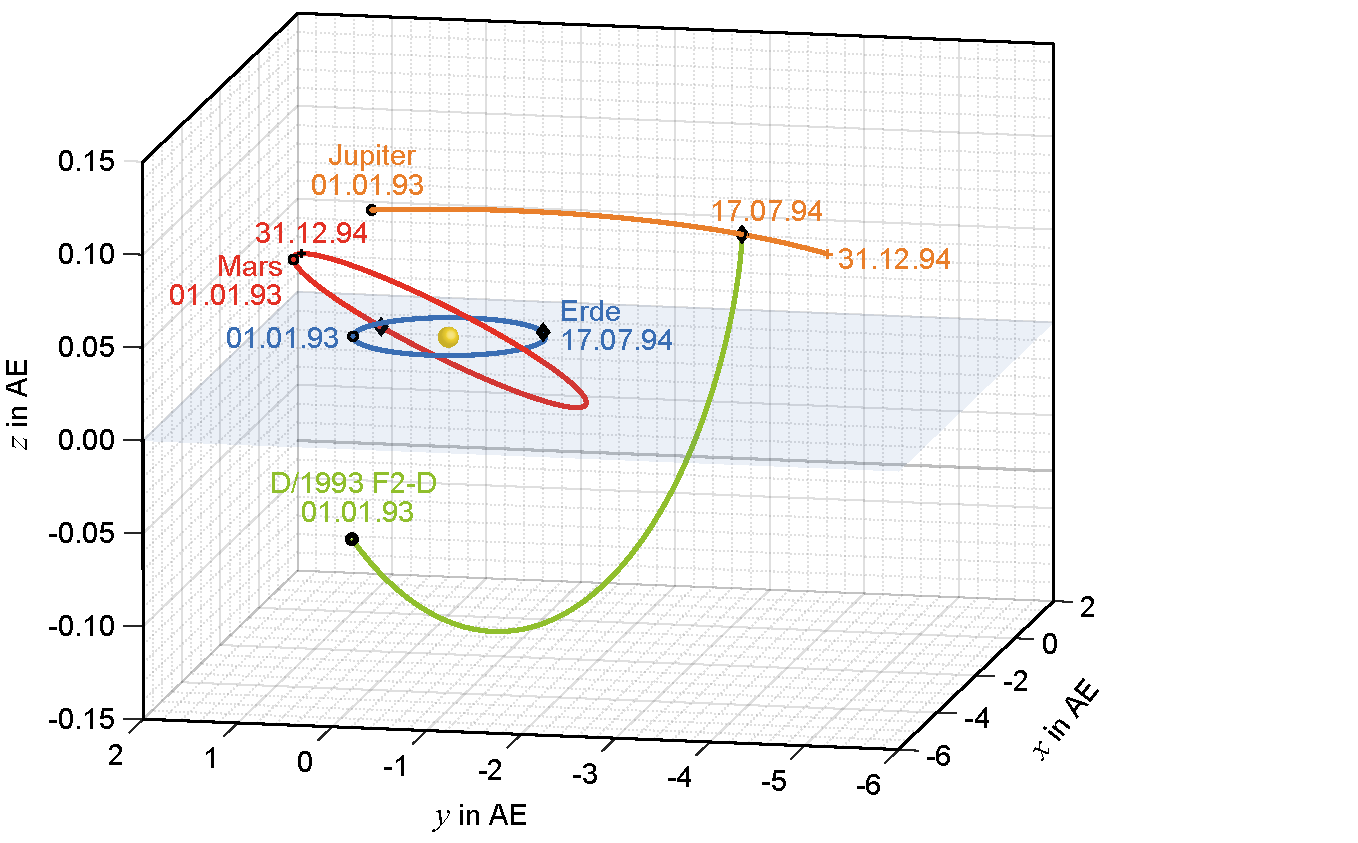
\includegraphics[width=\columnwidth]{SL9b_Variante.pdf} 
\captionof{figure}[Bahn des Kometen Shoemaker-Levy 9 in den Jahren 1993/94.]{Bahn des Kometen Shoemaker-Levy 9 in den Jahren 1993/94 bis zum Aufschlag auf den Jupiter.}\label{abb:hm_SL9Bahn}
\end{center}

Die Rechnung zeigt, dass der Komet sich bereits zu diesem Zeitpunkt im \anf{Einfangbereich} des Jupiters befand und dass eine dramatische Zunahme der Kr�fte des Jupiters $F_{\jupiter}$ zu erwarten war. 
Wir k�nnten nun mit den Anfangswerten an die L�sung des Dreik�rperproblems mit dem bekannten und in den \onlineZ{} beschriebenen \textit{Runge-Kutta-Verfahren}\index{Runge-Kutta-Verfahren} gehen, k�nnen das Problem aber etwas vereinfachen, da wir die Bahn des Jupiters als weiterhin ungest�rt annehmen k�nnen.
Wir benutzen deshalb in \mlhmref{SL9numerisch.m} auch die in \matlab{} hinterlegten Routinen (\zb \textcolor{mygreen}{\texttt{ode45}}) zur L�sung des Differentialgleichungssystems f�r $\vec{\psi}(t)$.
Das Ergebnis der Berechnung ist in \figref{hm_SL9Bahn} zu sehen.
Mit guter Genauigkeit berechnet das Programm den Zusammenprall von SL9 (D/1993 F2) f�r den 17.\,07.\,1994 um 20:35 UT.
Der so berechnete Zeitpunkt weicht nur wenig vom tats�chlich beobachteten Zeitpunkt 18.\,07.\,1994, 00:35 UT ab. 
Aus den Rechnungen wird allerdings auch deutlich, wie extrem kritisch die Ergebnisse von den Anfangsparametern (Ort und Geschwindigkeit des Kometen) und der Masse des Jupiters abh�ngen.
In \figref{hm_SL9Bahnberechnung} haben wir diese Parameter etwas variiert.
Es zeigt sich, dass im Fall einer h�heren Jupitermasse der Komet erwartungsgem�� fr�her auf den Jupiter aufschlagen w�rde.
In den F�llen der um 20\% erh�hten oder ver�nderten Anfangsgeschwindigkeiten des Kometen w�rde dieser den Jupiter aber \anf{verfehlen}.
Dies zeigt noch einmal deutlich, wie wichtig hochgenaue Beobachtungsdaten f�r Berechnungen in der Himmelsmechanik sind. \\

\begin{center}
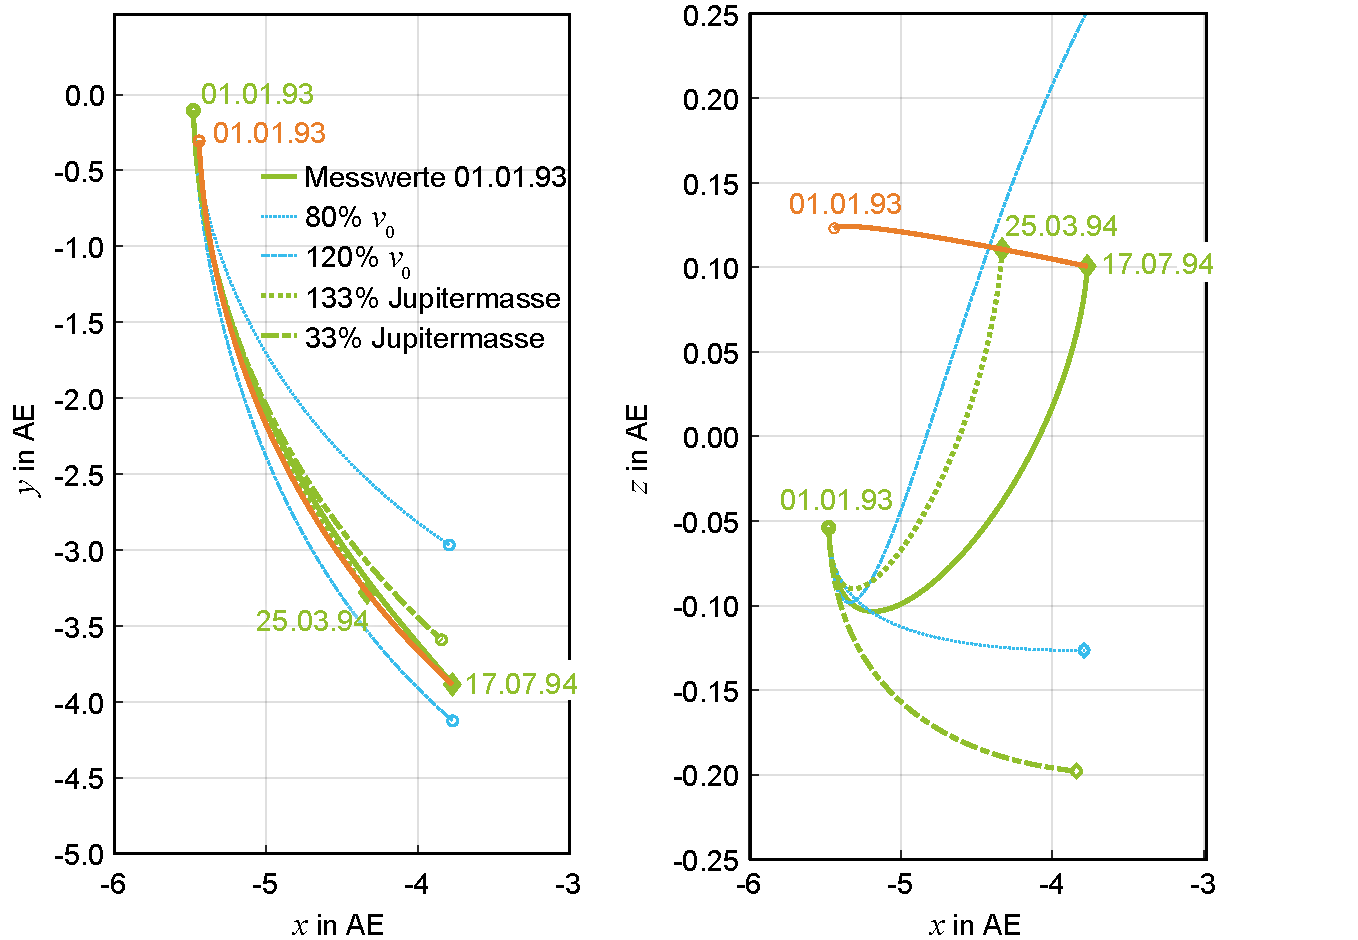
\includegraphics[width=\textwidth]{SL9a.pdf}
\captionof{figure}[Bahnberechnung des Kometen Shoemaker-Levy 9 in den Jahren 1993/94.]{Bahnberechnung des Kometen Shoemaker-Levy 9 in den Jahren 1993/94 mit verschiedenen Annahmen f�r Jupitermasse und Anfangsgeschwindigkeiten.}\label{abb:hm_SL9Bahnberechnung}
\end{center}

Zum Schluss berechnen wir noch, mit welcher Geschwindigkeit der Komet auf den Jupiter prallt.
Unsere numerischen Rechnungen ergeben f�r den letzten Rechenschritt vor dem Zusammenprall 
\begin{align*}
\vec{v}_\text{SL9} &= \lk \begin{array}{c} +0.013395176\\ +0.006460533 \\ -0.029725683 \end{array}\rk \:\text{AE/d} \;\: \text{bzw.}\ \;\vec{v}_{\jupiter} = \lk \begin{array}{c} +0.005323551\\ -0.004907594 \\ -0.000098762 \end{array}\rk \:\text{AE/d} 
\end{align*}
eine Aufprallgeschwindigkeit von
\begin{equation*}
  v_\text{impact} = \sqrt{\left|{\vec{v}_\text{SL9}-\vec{v}_{\jupiter}}\right|^2} \approx \SI{57.1}{\kilo\metre\per\second}~.
\end{equation*}
Diese Geschwindigkeit liegt nahe an der 2.~kosmischen Geschwindigkeit\index{Geschwindigkeit!2.~kosmische} des Jupiters von 
\begin{equation*}
  v_\text{escape} = \sqrt{\frac{2 G\, m_{\jupiter}}{R_{\jupiter}}}\approx \SI{59.5}{\kilo\metre\per\second}~,
\end{equation*}
was verst�ndlich ist, da der Komet den Jupiter auf dessen Bahn unter einem Winkel von nahezu $90\degree$ trifft.
Hierin ist $R_{\jupiter}$ der Radius des Jupiters.
Aus \cite{Crawford1996} k�nnen wir die Gesamtgr��e des Kometen vor dem Zerbrechen mit $\SI{1.4}{\kilo\metre}$ entnehmen.
Mit einer mittleren Dichte von $\SI{0.5}{\gram\per\centi\metre^3}$ ergibt sich daraus eine kinetische Aufprallenergie von $\SI{1.17e21}{\joule}$.
Das entspricht einer unglaublichen \anf{Explosionskraft} von \ca \SI{280}{\giga\tonne} TNT, was gleichbedeutend mit der Sprengkraft von etwa 18 Millionen Hiroshima-Bomben ist.\\

\end{example}
%%BEISPIEL %%%%%%%%%%%%%%%%%%%%%%%%%%%%%%%%%%%%%%%%%%%%%%%%%%%%%%%%%%%%%%%%%%%%%%%%%%%%%%%%%%

Obwohl offensichtlich ist, dass die in Beispiel \ref{bsp:hm_shoemaker_levy} berechnete Bahn des Kometen erheblich von einer reinen Keplerbahn abweicht, werden wir im \kap{kometen} sehen, dass man f�r n�herungsweise Berechnungen von weniger gest�rten Kometenbahnen durchaus die Keplerl�sung mit effektiven Bahnparametern benutzen kann.
\subsection{Periheldrehung des Merkurs}\index{Periheldrehung} \label{kap:Periheldrehung}
Wie wir gesehen haben, gibt es gravitative Einfl�sse der anderen Planeten auf ein ideales ZKP (reines Sonne-Planet-System), die zu St�rungen der reinen Keplerl�sungen und -ellipsen f�hren.
Wir wollen eine dieser St�rungen -- die auch wissenschaftshistorisch sehr interessant ist -- in diesem Kapitel etwas genauer betrachten.
Wir m�chten uns aber zun�chst der Frage zuwenden, unter welchen Bedingungen wir bei vorhandenen St�rungen �berhaupt von stabilen und geschlossenen Bahnen sprechen k�nnen.
Unter \anf{stabil} verstehen wir, dass der Radius $r$ der Bahn �ber die Zeit in einem endlichen Bereich bleibt.
Unter \anf{geschlossen} verstehen wir, dass es einen ausgezeichneten Punkt der Bahn gibt (\zb das Perihel), der sich nach einem vollen Umlauf $T_\text{P}$ wieder an derselben Position befindet, also $\lek r(t_0+T_\text{P}), \upsilon(t_0+T_\text{P})\rek\!=\!\lek r(t_0), \upsilon(t_0) \rek$.

\subsubsection{Bedingungen f�r stabile und geschlossene Bahnen}\index{Bahn!geschlossene}\index{Bahn!stabile} \label{kap:Stabile_Bahnen}
Wir wollen nun ein allgemeines Gravitationspotential $U_\text{\,ZK}(r)$ annehmen, welches aber immer noch ein \gls{zkf}\index{Zentralkraftfeld} (ZK) repr�sentiert.
Die Bewegung findet wegen der weiterhin geltenden Drehimpulserhaltung in einer Ebene statt.
Die Bewegung eines Planeten mit Masse $m$ in diesem ZK kann durch folgendes Potential eines Gravizentrums\footnote{Hierbei haben wir wie bisher auch das \pot{} auf die Masse $m$ \anf{normiert}. Wir werden sp�ter im Kapitel, wenn es um die Berechnung von Merkur-Messwerten geht, die entsprechenden Gr��en mit der Masse des Merkurs $m_{\mercury}$ multiplizieren.} beschrieben werden:
\begin{align}
%U_\text{Z}(r) &= -\frac{\mu_\text{G}}{r} + \frac{\kappa_2}{r^2} + \frac{\kappa_3}{r^3} +\ldots = -\frac{\mu_\text{G}}{r} + \sum \limits_{i}{} \Delta U_i(r) \,, \label{eq:hm_bwg_allg_ZK}
U_\text{\,ZK}(r) &= -\frac{\mu_\text{G}}{r} + \sum \limits_{i}{} \Delta U_i(r) \,. \label{eq:hm_bwg_allg_ZK}
\end{align}
Daraus ergibt sich folgende allgemeine Bewegungsgleichung:
\begin{equation}
%\vec{b}_\text{\,ZK}(r) & = \frac{\vec{F}_\text{\,ZK}}{m} = 
\ddot{\vec{r}} = -\frac{\d U_\text{\,ZK}(r)}{\d r} \lk \frac{\vec{r}}{r} \rk = \lek - \frac{\mu_\text{G}}{r^2} + \sum \limits_{i}^{} \Delta g_i(r) \rek \vec{e}_r \label{eq:hm_bwg_allg_ZK2}
\end{equation}
mit $\Delta g_i(r)\!=\!-\d \Delta U_i(r)/\d r$.
Die Zusatzterme im Potential $U_\text{\,ZK}(r)$ sollen als klein angenommen werden.
Wir k�nnen dann die Methoden der St�rungsrechnung verwenden.
Bisher sind wir stillschweigend davon ausgegangen, dass die St�rungen so beschaffen sind, dass man weiterhin von nur leicht ver�nderten Keplerbahnen sprechen kann.
Bevor wir an die Bahnberechnung gehen, m�chten wir das aber jetzt genauer untersuchen und ein paar allgemeine Erkenntnisse zur Stabilit�t von Planetenbahnen ableiten.
In Polarkoordinaten kann eine Kraft geschrieben werden als
\begin{equation*}
\vec{F} = F_r\,\vec{e}_r + F_\upsilon\,\vec{e}_\upsilon\,.
\end{equation*}
Bei der Betrachtung der Stabilit�t einer Bahn interessiert uns nur der Betrag der Radialkomponente $F_r$ der Kraft \bzw Beschleunigung, die geschrieben werden kann als
\begin{equation}
b_r(r) = b(r) = \frac{F_r(r)}{m} = \frac{\d U_\text{\,ZK}(r)}{m\,\d r} = \ddot{r}-\dot{\upsilon}^2 r \,. \label{eq:hm_b_r_1}
\end{equation}
Mit dem ebenfalls auf die Masse $m$ normierten Drehimpuls $L\!=\!r^2\dot{\upsilon}$ \eqref{eq:hm_drehimp_z_polar} folgt daraus
\begin{equation}
b(r) = \ddot{r} - \frac{L^2}{r^3}\,. \label{eq:hm_b_r_2}
\end{equation}
Wir betrachten zun�chst nahezu kreisf�rmige Bahnen, f�r die wegen $r=a$ und damit $\ddot{r}\!=\!0$
\begin{equation}
b(a) = -\frac{L^2}{a^3} \label{eq:hm_b_r_3}
\end{equation}
gilt. Nehmen wir nun eine leichte St�rung des Planeten an, dann ist es gerechtfertigt, dessen Bahnbewegung als eine kleine Oszillation $\xi\!=\! r-a$ um den Radius $a$ zu betrachten.
Wir k�nnen dann die Bewegungsgleichungen \eqref{eq:hm_b_r_2} linearisieren.
Mit $\ddot{a}\!=\!0$ und $\xi\!\ll\! a$ folgt
\begin{equation}
	b(\xi+a) = \ddot{\xi} - \frac{L^2}{(\xi+a)^3} \approx \ddot{\xi} - \frac{L^2}{a^3} \lk 1-\frac{3\xi}{a} + \mathcal{O}(\xi^2) \rk ~. \label{eq:hm_b_r_4}
	%= \ddot{\xi} - \frac{L^2}{a^3}\lk 1+\frac{\xi}{a}\rk^{-3} 
	\end{equation}
Andererseits k�nnen wir die linke Seite von $b(\xi+a)$ in \eqref{eq:hm_b_r_4} als Taylorentwicklung $b(\xi+a)= b(a) + \xi \, b'(a)$ schreiben:
\begin{align*}
	b(a) + \xi b'(a) &= \ddot{\xi} + b(a)\lk 1 - \frac{3\xi}{a}\rk ~,
\end{align*}
woraus eine Differentialgleichung f�r die St�rung $\xi(t)$
\begin{align}
	\ddot{\xi} + \xi\lek -\frac{3}{a} b(a) + b(a) - b(a) - b'(a) \rek &= 0 \nonumber\\
	\Rightarrow \ddot{\xi} + \xi\lek \lk -\frac{3}{a}\rk b(a) - b'(a) \rek &= 0 \label{eq:hm_Stoer_1} ~~
\end{align}
folgt.
Das ist eine harmonische Schwingungsgleichung, deren L�sung mit der Frequenz 
\begin{equation}
\omega = \sqrt{\lk -\frac{3}{a} \rk b(a) - b'(a)} \label{eq:hm_lsg_Stoer}
\end{equation}
durch
\begin{equation*}
\xi = A\E^{i\omega t} + B\E^{-i\omega t} 
\end{equation*}
gegeben ist.
Wir erhalten eine erste Bedingung f�r die Stabilit�t einer Bahn.
Stabile (d.\,h. auch periodisch oszillierende) Bahnen sind nur m�glich, wenn $\omega$ in \eqref{eq:hm_lsg_Stoer} reell ist, was auf folgende Forderung an die Charakteristik des Zentralkraftfeldes f�hrt:
\begin{equation}
\frac{F_r(a)}{m} = b(a) < \frac{a \, b'(a)}{3} \,.\label{eq:hm_stab_bedingung}
\end{equation}
Bei imagin�rem $\omega$ hingegen wird die Bahn instabil.
Man rechnet leicht nach, dass f�r das Newtonsche Gravitationsgesetz Bedingung \eqref{eq:hm_stab_bedingung} erf�llt ist.\footnote{In \probref{hm_hill_sphere} stellen wir f�r ein spezifisches Dreik�rperproblem eine detaillierte Stabilit�tsbetrachtung an.}
Das gilt auch f�r allgemeinere F�lle nach Gleichung \eqref{eq:hm_bwg_allg_ZK}, sofern die Potential-Anteile  $\Delta U_i(r)$ des ZK bestimmte Verh�ltnisse und Vorzeichen haben.
Aber selbst im Fall eines reellen $\omega$ wird die Bahn im Allgemeinen nicht mehr vollst�ndig geschlossen sein.
Das wird beispielsweise deutlich, wenn man die wahre Anomalie $\upsilon_{\text{P}_0}\!=\!\dot{\upsilon}\, 2\pi/\omega = \!\dot{\upsilon}\, T_\text{P}$ berechnet.
Diese entspricht dem vom Radiusvektor in einer Periode $T_\text{P}$ zu \anf{identischen} Radien der Bahn (\zb dem Perihel) �berstrichenen Winkel, der sich mit \eqref{eq:hm_lsg_Stoer} und \eqref{eq:hm_b_r_3} und  $L\!=\!\sqrt{-b(a)\,a^3}$ berechnet zu
\begin{align}
	\upsilon_{\text{P}_0} &= \frac{2\pi}{\omega}\frac{L}{a^2} = \frac{2\pi}{\omega}\frac{\sqrt{-b(a)\,a^3}}{a^2} = \frac{2\pi}{a^2}\,\frac{\sqrt{-b(a)\, a^3}}{\sqrt{\lk -\frac{1}{a}\rk \lek 3b(a) + a\,b'(a) \rek}} \nonumber\\
	\Rightarrow \upsilon_{\text{P}_0} &= 2\pi\,\frac{1}{\sqrt{3+a\,\frac{b'(a)}{b(a)}}} = \frac{2\pi}{\gamma} \,. \label{eq:hm_upsilon_P0}
\end{align}
Die Winkeldifferenz $\Delta\upsilon_{\text{P}_0}\!=\!\upsilon_{\text{P}_0} - 2\pi$ bezeichnen wir als Perihelverschiebung\index{Perihelverschiebung|textbf}.
Sie wird h�ufig auch als \emph{Perihelpr�zession}\index{Perihelpr�zession} bezeichnet. 
\begin{figure}
\begin{minipage}{\textwidth}
\leftfigure{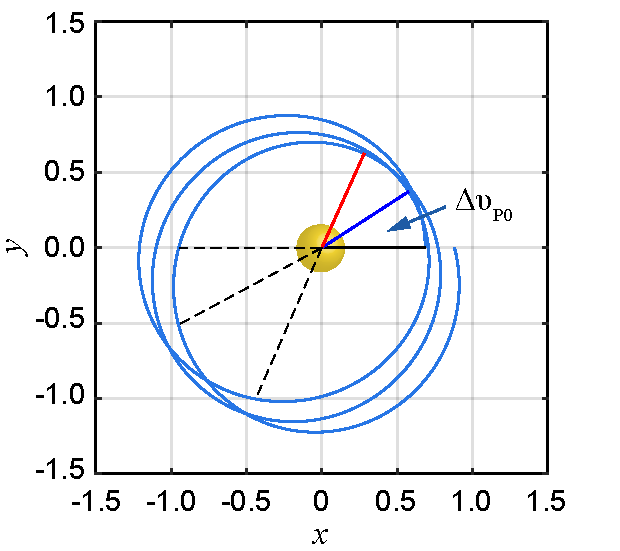
\includegraphics[width=0.5\textwidth]{Perihel01.pdf}}
\hspace{\fill}
\rightfigure{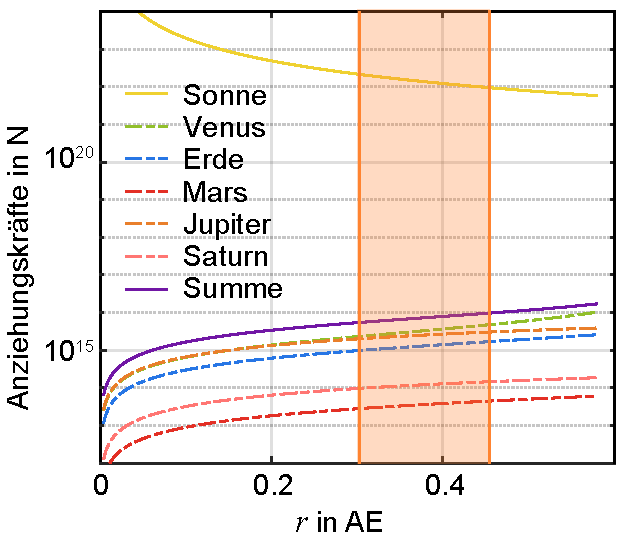
\includegraphics[width=0.5\textwidth]{StoerpotentialMerkur.pdf}}
\leftcaption{Periheldrehung.}\label{abb:hm_perihel_01}
\rightcaption[Anziehungskr�fte auf den Merkur durch die Sonne und �u�ere Planeten.]{Anziehungskr�fte auf den Merkur durch die Sonne und die �u�eren Planeten. Schattiert ist der Aufenthaltsbereich des Merkurs gezeigt. Man beachte die Gr��enunterschiede im Betrag von Sonne zu Planeten von $\approx \SI{1e6}{}$.}\label{abb:hm_stoerpotential_merkur}
\end{minipage}
\end{figure}

Aus \eqref{eq:hm_upsilon_P0} erkennen wir, dass $\upsilon_{\text{P}_0}$ nach einer Periode nur dann gleich $2\pi$ ist, wenn 
\begin{equation}
\gamma = 3+a\,\frac{b'(a)}{b(a)} \equiv 1 \,. \label{eq:hm_perihel_bed}
\end{equation}
F�r die Newtonsche Gravitationskraft $\mu{_\text{G}}/a^2$ (normiert auf die Masse $m$) ist $b(a)\!=\!-1/a^2$ und $b'(a)\!=\!2/a^3$. F�r diesen Fall folgt dann
\begin{equation*}
3+a\lk \frac{2}{a^3}\rk \lk-\frac{a^2}{1} \rk = 1 \,
\end{equation*}
und damit keine Perihelverschiebung. F�r jedes von $r^{-2}$ abweichende Kraftfeld ergibt die linke Seite von \eqref{eq:hm_perihel_bed} einen Wert $\neq\! 1$ und damit nach \eqref{eq:hm_upsilon_P0} mit $\upsilon_{\text{P}_0}\!\neq\!2\pi$ (\probref{hm_potential_merkur}) eine nicht mehr vollst�ndig geschlossene Bahn.
So ist \zb das Perihel nach einem vollen Umlauf nicht mehr bei der gleichen Anomalie zu finden.
Es hat sich etwas verschoben \bzw verdreht, ebenso wie die Apsidenlinie (\figref{hm_perihel_01}).\footnote{Wir haben die Stabilit�tsbedingung \eqref{eq:hm_stab_bedingung} und auch die Beziehung f�r die Perihelverschiebung \eqref{eq:hm_upsilon_P0} auf Basis ann�hernd kreisf�rmiger Bahnen abgeleitet \cite{Price1979}.
Sie gelten aber im Prinzip genauso f�r elliptische Bahnen. Wir verweisen hierzu auf \cite{Davies1983}.} 

\subsubsection{Berechnung des St�rpotentials und der Periheldrehung f�r den Planeten Merkur\, ($\mercury$)}\index{St�rpotential} \label{kap:Stoerpotential_Merkur}
Die Frage ist nun, wie solche Zusatzpotentiale $\Delta U_i(r)$ in der Realit�t beschaffen sind und ob man eine solche Verschiebung des Perihels berechnen und messen kann.
Wir m�chten mit einem einfachen physikalischen Modell das St�rpotential f�r den Merkur berechnen.
F�r diesen muss sich das gr��te St�rpotential ergeben, da alle anderen Planeten au�erhalb seiner Bahn liegen und damit der Anziehung des Merkurs durch die Sonne entgegen wirken.
Unser Modell f�r das St�rpotential \cite{Price1979, Davies1983} beruht auf der Annahme, dass die zeitlich gemittelten St�rungen der anderen Planeten auf den Merkur jeweils durch das Potential eines massebeladenen Rings mit Radius $a_k$ der jeweiligen Planetenbahn und der Ring-Massendichte $\rho_k=m_k/{2\pi a_k}$ mit $k=2 \ldots 8$ gegeben ist.
Hier ist $m_k$ die Masse des $k$-ten Planeten, wobei man aber wegen der verschwindenden Beitr�ge von Uranus und Neptun nur bis $k\!=\!6$ (also bis zum Saturn) aufsummieren muss.
Der Vorteil dieser Herangehensweise ist, dass man mit der oben abgeleiteten Beziehung \eqref{eq:hm_upsilon_P0} die Perihelverschiebung\index{Perihelverschiebung} $\Delta \upsilon_{\text{P}_0}$ n�herungsweise berechnen kann, ohne die komplexe Bewegungsgleichung explizit l�sen zu m�ssen.
Die mittleren Beschleunigungen der anderen Planeten auf den Merkur k�nnen entsprechend dieses Ringmodells nach folgender Formel aufsummiert werden (\probref{hm_potential_merkur}):
\begin{equation}
\Delta g_{\,\mercury}(r) = G \pi \sum \limits_{k=2}^{6} \lk \frac{m_k}{2\,\pi\,a_k} \rk \frac{r}{a_k^2 - r^2} \,.
\label{eq:hm_merkur_mittlere_beschl}
\end{equation}
Hierin ist $r$ der Bahnradius des Merkurs \cite{Price1979}.
Die nach diesem Modell des massebehafteten Rings berechnete Gravitationskraft der �u�eren Planeten auf den Merkur ist tats�chlich eine Zentralkraft (\figref{hm_stoerpotential_merkur}) und muss (da alle $a_k\!>\!r_{\mercury}$ sind) eine absto�ende Kraft sein, \dh sie wirkt der anziehenden Gravitationskraft der Sonne entgegen.
F�r das Potential k�nnen wir schreiben:
\begin{align}
	\Delta \,U_{\,\mercury}(r) &= -G \pi \sum \limits_{k=2}^{6} \lk \frac{m_k}{2\,\pi\,a_k^3} \rk \bigintsss \frac{r}{\lk 1 - \frac{r^2}{a_k^2}\rk}\,\D r \nonumber \\
	&= \frac{1}{2} G \pi \sum \limits_{k=2}^{6} \lk \frac{m_k}{2\,\pi\,a_k} \rk \log \lk 1- \frac{r^2}{a_k^2} \rk \nonumber \\
	&\approx \frac{1}{2} G \pi \sum \limits_{k=2}^{6} \lk \frac{m_k}{2\,\pi\,a_k} \rk \lek \frac{r^2}{a_k^2} + \mathcal{O}\lk \frac{r^4}{a_k^4}\rk \rek \,. \label{eq:hm_merkur_mittleres_potential}
\end{align}
Setzt man in \eqref{eq:hm_merkur_mittlere_beschl} die Werte f�r $a_k, m_k$ aus Tabelle \ref{tab:hm_bahnparameter} aus dem Tabellenanhang ein und ebenso  $r\!=\!a_{\mercury}$, dann erh�lt man  f�r das Verh�ltnis der Zusatzkraft zur Anziehungskraft der Sonne
\begin{equation*}
\frac{\Delta g_{\,{\mercury}} (a_{\mercury})}{-\mu_G/a_{\mercury}^2} \:\approx \:-\frac{\pi}{m_{\astrosun}} \, a_{\mercury}^2\, 100 \:\text{kg\,m}^{-2} \approx - \SI{6e-7}{} \,.
\end{equation*}
Das ist im Verh�ltnis zur Anziehung durch die Sonne eine sehr kleine absto�ende St�rung (Man beachte die logarithmische Darstellung in \figref{hm_stoerpotential_merkur}.).
Wir werden aber gleich sehen, welche doch messbare Wirkung dieses geringe resultierende Potential hat und vor allem auch wissenschaftshistorisch hatte.
Wir berechnen dazu f�r die Merkurbahn die Gr��en $b(a)$ und $b'(a)$, die wir f�r \eqref{eq:hm_upsilon_P0} brauchen:
\begin{align*}
		m_{\mercury} \, b_{\mercury}(a_{\mercury}) &= \underbrace{-\frac{\mu_\text{G} \, m_{\mercury}}{a_{\mercury}^2}}_{F_0 \approx \SI{-1.31e22}{}\:\text{N}} + \underbrace{m_{\mercury} \, \Delta \,g_{\,{\mercury}} (a_{\mercury})}_{\Delta F \approx \SI{7.56e15}{} \text{N}} ~, \nonumber \\  
	m_{\mercury} \, b'_{\mercury}(a_{\mercury}) \, a_{\mercury} &= \underbrace{+\frac{2 \mu_\text{G} \, m_{\mercury}}{a_{\mercury}^2}}_{-2 \, F_0} + \underbrace{m_{\mercury} \, a_{\mercury} \, \frac{\d }{\d r} \lk \Delta \,g_{\,{\mercury}}(r) \rk \bigg|_{r=a_{\mercury}}} _{\mu_\text{G} \pi\, a_{\mercury} \, m_{\mercury} \, S(r)}  
\end{align*}
mit der Summe
\begin{equation*}
	S=S(a_{\mercury})=\sum\limits_{k=2}^{6}\lk \frac{m_k}{2\pi \, {r_k}^2} \rk \frac{{r_k}^2+{a_{\mercury}}^2}{\lk {r_k}^2-{a_{\mercury}}^2 \rk^2}\,.
\end{equation*}
Das setzen wir in \eqref{eq:hm_upsilon_P0} ein und erhalten f�r die wahre Anomalie
\begin{align}
	\upsilon_{\text{P}_0} &= 2\pi \lk {3 + \frac{-2 F_0 + G\pi \, a_{\mercury}\, m_{\mercury} \, S}{F_0+\Delta F} }\rk^{-\frac{1}{2}} \nonumber \\
	  & = 2\pi \lk {\frac{1+ 3 \frac{\Delta F}{F_0} + \frac{1}{F_0}\, G\pi \, a_{\mercury}\, m_{\mercury} \, S}{1 +\frac{\Delta F}{F_0}} }\rk^{-\frac{1}{2}} \nonumber\\
		&\approx 2\pi \lk { 1 - \frac{\Delta F}{F_0} - \frac{G\pi \, a_{\mercury}\, m_{\mercury} \, S}{2F_0} }\rk + \mathcal{O}\lk {\lk \frac{\Delta F}{F_0}\rk^2}\rk \,. \label{eq:hm_mercury_perihel_shift1}
\end{align}
Mit den Daten des Merkurs $a_{\mercury}$, $m_{\mercury}$, den Werten f�r $F_0, \Delta_F$ und $S$ (siehe \mlhmref{StoerpotentialMerkur.m}), sowie der siderischen Umlaufzeit des Merkurs von 87.969 d berechnen wir f�r die Verschiebungsrate $\Delta \dot{\upsilon}_{\text{P}_0}$ des Perihels 
\begin{align}
\begin{split}
	\Delta \dot{\upsilon}_{\text{P}_0} &= \frac{\upsilon_{\text{P}_0} - 2 \pi}{T_{\mercury}}  \\
	&= \frac{\Delta \upsilon_{\text{P}_0}}{T_{\mercury}} = \frac{2 \pi}{F_0 T_{\mercury} } \, \lk{- \Delta F - \frac{1}{2} G\pi a_{\mercury} m_{\mercury} S}\rk \approx 531.5''/\text{Jh.} 
\end{split} \label{eq:hm_mercury_per_shift2}
\end{align}
Das Ergebnis der Berechnung der Potentialanteile der einzelnen Planeten ist in \mlhmref{StoerpotentialMerkur.m} ausgef�hrt und in \figref{hm_stoerpotential_merkur} dargestellt.\\
Wir haben mit relativ einfachen �berlegungen eine gute Absch�tzung f�r die Perihelverschiebung f�r ann�hernd kreisf�rmige Bahnen erhalten.\footnote{Unsere Betrachtungen zur Absch�tzung der Perihelverschiebung beruhten auf der N�herungsannahme kreisf�rmiger Bahnen \cite{Price1979, Stump1988}.
In \cite{Davies1983} und \cite{Stewart2005} wird eine Erweiterung auf elliptische Bahnen angegeben.
Der Effekt ist aber relativ klein ($<\! 1''$).
Unsere N�herung war also gerechtfertigt.} Es w�re aber doch sch�n, wenn wir auch die Bahn explizit als Funktion der Zeit berechnen k�nnten. Das wollen wir in \probref{hm_perihel_kappa3} tun.\\


\subsubsection{Bahnberechnung f�r ein verallgemeinertes Zentralkraftfeld}\index{Zentralkraftfeld} \label{kap:Allg_ZK__Merkur}
Mit \eqref{eq:hm_merkur_mittleres_potential} haben wir das St�rpotential (\bzw Kraftfeld) f�r den Merkur in einer Form bestimmt, die leider keine direkte Integration der Bewegungsgleichung erlaubt.
Man ist also auf St�rungsrechnungen angewiesen.
Wir wollen aber zun�chst f�r Potentiale, die sich als Reihenentwicklung von $r^{-n}$ darstellen lassen, einen analytischen Ansatz versuchen.
Wir schreiben dazu \eqref{eq:hm_bwg_allg_ZK} in folgender Form:
\begin{align}
	U_\text{\,ZK}(r) &= -\frac{\mu_\text{G}}{r} + \Delta U_2 + \Delta U_3 = -\frac{\mu_\text{G}}{r}  + \frac{\kappa_2}{r^2} + \frac{\kappa_3}{r^3} + \ldots \,.
	\label{eq:hm_allg_ZK_1}
\end{align}
Die spezifische, wiederum auf die Masse $m$ normierte Gesamtenergie des Systems $H$ in Polarkoordinaten ist dann mit \eqref{eq:hm_bewgl1} gegeben durch
\begin{equation}
	H = \frac{1}{2} (\dot{r}^2 + r^2\dot{\upsilon}^2) + U(r) \,. \label{eq:hm_total_energy}
\end{equation}
Mit dem Drehimpuls $L = r^2\dot{\upsilon}$ aus \eqref{eq:hm_drehimp_z} schreiben wir $\dot{\upsilon}\!=\!L/r^2$ und setzen das in die Gleichung f�r die Energie \eqref{eq:hm_total_energy} ein:
\begin{align}
  H &= \frac{1}{2} \dot{r}^2 + \frac{r^2}{2} \frac{L^2}{r^4} + U(r)
      \qquad \Rightarrow \qquad
      \dot{r}^2 = 2H - 2 \underbrace{\lk \frac{L^2}{2 r^2} + U(r) \rk}_{U_\text{eff}} \nonumber \\
\Rightarrow \dot{r} &= \sqrt{2 H - 2 \lk \underbrace{-\frac{\mu_\text{G}}{r} + \frac{L^2}{2r^2}}_{U_\text{eff, K}} + \underbrace{\frac{\kappa_2}{r^2}}_{\Delta U_1} + \underbrace{\frac{\kappa_3}{r^3}}_{\Delta U_2} \rk} ~. \label{eq:hm_allg_ZK_2}
\end{align}
Hierin sind $U_\text{eff,K}(r)$ und $U_\text{eff}(r)$ das effektive Potential des Keplerproblems \bzw des allgemeinen ZK-Feldes, wobei
\begin{equation*}
U_\text{eff,K}(r)\!=\! -\frac{\mu_\text{G}}{r} + \frac{L^2}{2r^2} ~ \;~\text{und}\;~ U_\text{eff}(r) = U_\text{eff,K}(r) + \Delta U_2 + \Delta U_3 ~~   \,.
\end{equation*}
Um $r(\upsilon)$, \dh die Bahn zu berechnen, schreiben wir die Zeitableitung des Bahnradius als
\begin{align*}
	\dot{r} &= \frac{\D r}{\D t} = \frac{\D r}{\D \upsilon}\frac{L}{r^2} = \sqrt{2\lk H - U_\text{eff}(r)\rk} ~,\\
\text{woraus}~~ \D \upsilon &= \frac{L\,\D r}{r^2\sqrt{2 \lk H - U_\text{eff}(r)\rk}}  ~~\text{folgt.}
\end{align*}
Jetzt substituieren wir $r\!=\!1/q$ und $\D r = -1/q^2\,\D q$ und erhalten
\begin{align*}
\D \upsilon &= -\frac{L \killA{q^2}\,\D q}{\killA{q^2} \sqrt{2H - 2U_\text{eff}(q)}} = -\frac{\D q}{\sqrt{2H/L^2 - 2 U_\text{eff}(q)/L^2}} ~. 
\end{align*}
Das ergibt dann ausgeschrieben
\begin{align}
\upsilon &= - \bigintsss{\frac{L}{\sqrt{2H + 2\mu_\text{G}\, q - \lk L^2 + 2\kappa_2 \rk q^2 - 2\kappa_3\,q^3}}\, \D q } ~. \label{eq:hm_allg_ZK_3} 
\end{align}
Dieses Integral gilt es nun zu l�sen.
Wir haben das in Beispiel \ref{bsp:perihel_kappa2} f�r das St�rpotential $\kappa_2 /r^2$ ausgef�hrt.

%BEISPIEL 8 %%%%%%%%%%%%%%%%%%%%%%%%%%%%%%%%%%%%%%%%%%%%%%%%%%%%%%%%%%%%%%%%%%%%%%%%%%%%%%%%%%
\begin{example}{Integration der Bewegungsgleichung f�r ein ZK mit St�rpotential $\kappa_2/{r^2}$}
Wir setzen in \eqref{eq:hm_allg_ZK_3} $\kappa_3\!=\!0$, sodass wir ein leicht modifiziertes Keplerproblem erhalten.
Wir erkennen, dass im Fall $\kappa_2 \neq 0$ das effektive Keplerpotential des ungest�rten Falls $U_\text{eff, K}(r)$ durch einen Korrekturfaktor $2\kappa_2/L^2$ vergr��ert wird.
Wir k�nnten daher direkt die L�sung f�r die Bahn aus dem reinen ZKP nehmen und entsprechend modifizierte Parameter verwenden.
Wir wollen aber die Bahngleichung f�r das gest�rte System noch einmal explizit herleiten, da dies sehr instruktiv ist.
Dazu nutzen wir f�r \eqref{eq:hm_allg_ZK_3} die Abk�rzungen
\begin{align*}
	\hat{A} &= \frac{2H}{L^2} < 0 ~\text{, da die Ellipsenbahn gebunden ist} ~,\\
	\hat{B} &= \frac{2\mu_\text{G}}{L^2} > 0 \,, \\
	\hat{C} &= -\lk 1+\frac{2\kappa_2}{L^2}\rk < 0 ~\text{, da laut Voraussetzung }\frac{\kappa_2}{L^2}\ll 1 \,.
\end{align*}
In Integraltafeln finden wir f�r $\hat{C}\!<\!0$ und $\Delta\!=\!4\hat{A}\hat{C} - \hat{B}^2\!<\! 0$, was in unserem Fall erf�llt ist, f�r das Integral folgende L�sung:
\begin{align}
	\int \frac{1}{\sqrt{\hat{A} + \hat{B}q + \hat{C}q^2}} \,\D q &= \frac{-1}{\sqrt{-\hat{C}}}\,\arcsin\lk\frac{2\hat{C}q + \hat{B}}{\sqrt{-\Delta}}\rk \,. \label{eq:hm_allg_ZK_4}
\end{align}
In der L�sung \eqref{eq:hm_allg_ZK_4} des Integrals setzen wir
\begin{align}
D&=\sqrt{-\Delta}\!=\sqrt{\hat{B}^2-4\hat{A} \hat{C}} =\sqrt{\frac{8H}{L^2}\lk 1+ \frac{2\kappa_2}{L^2}\rk + \frac{4\mu_\text{G}^2}{L^4}} ~, \label{eq:hm_allg_ZK_5} \\
B&\!=\hat{B} ~ \text{und} ~ \nonumber \\
 C&\!=\!\sqrt{-\hat{C}}\!=\!\sqrt{1+2\kappa_2/L^2} \approx 1+\kappa_2/L^2~ . \nonumber 
\end{align}
Damit folgt 
\begin{align*}
	\upsilon-\upsilon_0 &= \frac{1}{C}\,\arcsin\lk \frac{B-2C^2 q}{D}\rk \bigg|^{q(\upsilon)}_{q_0} = \frac{1}{C}\,\arcsin\lk \frac{B-2C^2 \frac{1}{r}}{D}\rk \bigg|_{r_0}^{r(\upsilon)} \\
											&= \frac{1}{C}\,\arcsin \lk \frac{B-\frac{2C^2}{r}}{D} \rk - \underbrace{\frac{1}{C}\,\arcsin \lk \frac{B-\frac{2C^2}{r_0}}{D} \rk}_{\equiv K_0/C} ~~
\end{align*}
und umgeformt
\begin{equation*}
\sin\lek C(\upsilon-\upsilon_0) + K_0\rek	= \frac{B-\frac{2C^2}{r(\upsilon)}}{D} \,.  
\end{equation*}
Das ist schon eine Gleichung f�r die Bahn, allerdings noch eine implizite.
Wir wollen $r(\upsilon)$ explizit gewinnen und formen die Gleichung deshalb weiter um zu
\begin{equation*}
	r(\upsilon) = \frac{\frac{2C^2}{B}}{1-\frac{D}{B}\sin \lek C(\upsilon-\upsilon_0) + K_0\rek} ~. 
\end{equation*}
Wir w�hlen die Integrationskonstante $K_0$ ohne Beschr�nkung der Allgemeinheit so, dass sich 
\begin{equation*}
C\upsilon_0 - K_0 = \frac{\pi}{2} 
\end{equation*}
ergibt, denn dann ist $\sin\lk C \upsilon - C \upsilon_0 + K_0 \rk  = -\cos \lk C \upsilon \rk$, womit  wir schlie�lich erhalten:
\begin{equation}
	r(\upsilon) = \frac{\frac{2C^2}{B}}{1+\frac{D}{B}\,\cos(C\upsilon)} ~. \label{eq:hm_allg_ZK_6} 
\end{equation}
\label{bsp:perihel_kappa2}
\end{example}
%BEISPIEL %%%%%%%%%%%%%%%%%%%%%%%%%%%%%%%%%%%%%%%%%%%%%%%%%%%%%%%%%%%%%%%%%%%%%%%%%%%%%%%%%%

Schreiben wir \eqref{eq:hm_allg_ZK_6} aus dem Beispiel mit 
\begin{equation*}
C=\sqrt{1+2\kappa_2/L^2} \approx 1+ \frac{\kappa_2}{L^2} ~~
\end{equation*}
und unter Umbenennung der Parameter 
\begin{align*}
\frac{2C^2}{B} &= \hat{p} = \frac{L^2}{\mu_\text{G}} \lk {1+ \frac{2\kappa_2}{L^2}} \rk = p \lk {1+ \frac{2\kappa_2}{L^2}} \rk \,,\\
\frac{D}{B} &= \hat{e} = \sqrt{1 + \frac{2H L^2}{\mu_\text{G}^2} \lk 1 + \frac{2\kappa_2}{L^2} \rk} = e \sqrt{ 1 + \frac{4H\kappa_2}{\mu_\text{G}^2 e^2}}\,,
\end{align*} 
erhalten wir schlie�lich 
\begin{equation}
	r(\upsilon) = \frac{2C^2/B}{1+\frac{D}{B}\,\cos(C\upsilon)}=\frac{\hat{p}}{1+\hat{e}\cos(C\upsilon)} ~. \label{eq:hm_allg_ZK_7}
\end{equation}
Gleichung \eqref{eq:hm_allg_ZK_7} sieht genauso aus wie die Bahngleichung f�r die Ellipse im Keplerfall \eqref{eq:hm_kegelschnitt}, allerdings mit modifizierten Parametern.
Wir erkennen, wie nicht anders zu erwarten war, dass f�r $\kappa_2 \rightarrow 0$ die Werte in die bekannten Werte f�r das reine Keplerproblem �bergehen.
Beides ist nicht verwunderlich, da durch den $\kappa_2/r^2$-Term im Potential ja nur die Gr��e des effektiven Potentials ver�ndert wird, nicht aber die $r$-Abh�ngigkeit des Gesamtpotentials.
Durch den Zusatzterm wird quasi ein \anf{effektiver Drehimpuls} des Systems erzeugt.
Man sieht aber anhand von \eqref{eq:hm_allg_ZK_6}, dass durch diesen effektiven Drehimpuls der Term mit $\cos(C\upsilon)$ nicht mehr $2\pi$-periodisch bez�glich $\upsilon$ ist, $r(\upsilon)$ ist minimal f�r $\upsilon_{\text{P}_0}\!=\!0$ (Perihel) und maximal f�r $\upsilon_{\text{Ap}}\!=\!C /\pi$ (Aphel).
In einem Zeitintervall, das dann einem vollen Umlauf entspricht, nimmt also die wahre Anomalie um $2\pi/C$ zu.\footnote{Eigentlich m�sste man zeigen, dass die siderische Umlaufzeit f�r die gest�rte Keplerellipse gleich der des ungest�rten Falls ist. Das ist aber leicht einsichtig, da wegen der Drehimpulserhaltung auch im allgemeinen ZK-Feld weiterhin der Fl�chensatz gilt.}
Die Perihelverschiebung ergibt sich mit \eqref{eq:hm_allg_ZK_7} demnach zu 
\begin{equation}
\Delta \upsilon_{\text{P}_0} = 2\pi/C  - 2\pi=  2\pi \lk \frac{1}{\sqrt{1+2\kappa_2/L^2}} -1 \rk \approx -2\pi \frac{\kappa_2}{L^2} ~. 
\label{eq:hm_allg_ZK_8}
\end{equation}
Es ist interessant, dass die Perihel-�nderung umso kleiner ist, je gr��er der Drehimpuls ist.
Das ist aber einsichtig, denn die relative �nderung des effektiven Potentials gegen�ber dem reinen Keplerproblem ist bei gro�em Drehimpuls entsprechend kleiner.
Wir zeigen in \figref{hm_simulationen_merkur1} verschiedene mit \mlhmref{PerihelKappa2.m} berechnete Simulationen von Bahnkurven f�r ein Potential mit Zusatzterm $\kappa_2\!\neq\! 0$, wobei die Parameter bewusst unrealistisch gro� gew�hlt wurden, um die Effekte deutlich sichtbar zu machen. 

\begin{figure}
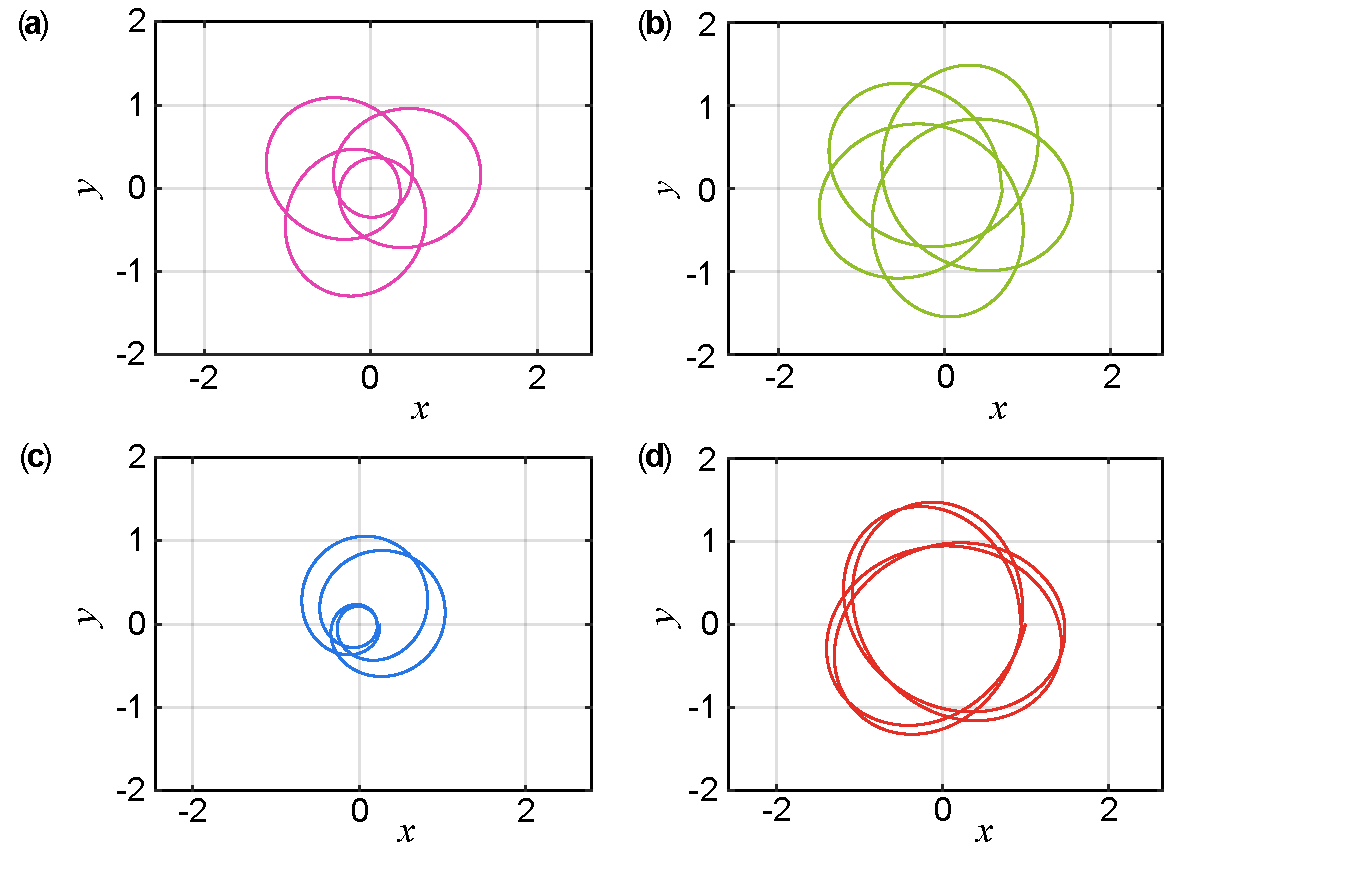
\includegraphics[width=\textwidth]{simulation_merkur1.pdf}%
\caption[Simulation von Bahnformen f�r verschiedene Parameters�tze.]{Simulation von Bahnformen f�r verschiedene Parameters�tze des Zentralkraftfeldes. Die Parameter sind $e=0.5, a = 1 $ und $\kappa_2 = -0.1\, \mu_\text{G}, + 0.1\, \mu_\text{G}, -0.2\, \mu_\text{G} \:\text{und}\: +0.2\,\mu_\text{G}$ f�r die Bilder \fa bis \fd. Um die Effekte deutlich sichtbar zu machen, wurden die Parameter unrealistisch gro� gew�hlt. Siehe \mscr~\mlhmref{PerihelKappa2.m}.}%
\label{abb:hm_simulationen_merkur1}%
\end{figure} 

\subsubsection{Merkur-Perihelverschiebung -- relativistischer Effekt}\index{Perihelverschiebung!relativistische} \label{kap:Relativistic_Merkur}
So sch�n und nachvollziehbar unsere Rechnungen zur Perihelverschiebung des Merkurs in \kapitel{Stoerpotential_Merkur} auch waren, die von vielen Astronomen mit Methoden der St�rungsrechnung sehr genau berechnet wurden, gibt es doch leider einen Haken.
Man fand n�mlich zwischen den berechneten ca. $531''$/Jh. und den tats�chlich beobachteten ca. $572''$/Jh. eine signifikante, nicht erkl�rbare Differenz von $41''$/Jh.
Auch der franz�sische Astronom Urbain Le Verrier\indexp{Le Verrier, Urrbain Jean Joseph}\footnote{Urbain Jean Joseph Le Verrier (1811--1877) war ein franz�sischer Astronom und Mathematiker. Ihm gelang 1846 die Vorausberechnung der vermutlichen Bahn des bis dahin unentdeckten Planeten Neptun aus den Bahnst�rungen des Uranus. Der Neptun wurde dann an der Berliner Sternwarte durch den Astronomen Galle mit dem 22-Zentimeter-Fraunhofer-Refraktor auch an der von Le Verrier vorhergesagten Position gefunden. Le Verrier gilt im �brigen auch als Erfinder der Wetterkarte.}, dessen genaue Berechnungen die Entdeckung des Neptuns erm�glicht hatten, konnte diese Diskrepanz nicht erkl�ren.
Er schlug vor, sicherlich durch den Erfolg beim Neptun ermutigt, nach einem inneren Planeten zu suchen.
Dieser erhielt den Namen Vulkan\footnote{Offensichtlich ein Vorgriff auf \emph{StarTrek}.}, er blieb allerdings im Gegensatz zum Neptun unauffindbar.
Die L�sung dieses R�tsels gelang erst Einstein\indexp{Einstein, Albert}\footnote{Albert Einstein (1879--1955) war einer der bedeutendsten Physiker der Weltgeschichte. Seine Forschungen zu Raum und Zeit,  sowie zum Wesen der Gravitation haben unser modernes Weltbild ma�geblich gepr�gt und seit Newton die wohl gr��te Revolution in der Physik eingeleitet.} mit seiner Arbeit zur \anf{Erkl�rung der Perihelbewegung des Merkur aus der allgemeinen Relativit�tstheorie} \cite{Einstein1915}.
Wir k�nnen hier leider nicht die Theorie darstellen.
Deshalb verweisen wir auf die entsprechenden Lehrb�cher \cite{Stephani1991, Moore2013}, k�nnen aber angeben, dass auf Basis der Allgemeinen Relativit�tstheorie die Bewegung eines K�rpers in einem ZKF durch folgende Bewegungsgleichung beschrieben werden kann: 
\begin{align}
\begin{split}
	\ddot{r} &=  -\frac{\mu_\text{G}}{r^2} + \lk 1- \frac{3\mu_\text{G}}{c^2 r} \rk \frac{L^2}{r^3} = -\frac{\mu_\text{G}}{r^2} + \frac{L^2}{r^3} - \frac{3\mu_\text{G} L^2}{c^2 r^4} \\
	&= -\frac{\mu_\text{G}}{r^2} + \frac{L^2}{r^3} - \frac{\d}{\d r} \Delta U_\text{rel}(r) 
\end{split} \label{eq:hm_einstein_01} 
\end{align}
mit $ \Delta U_\text{rel}(r) = -\mu_\text{G} L^2/(c^2 r^3) $. 
Die Bewegungsgleichung \eqref{eq:hm_einstein_01} wird in \probref{hm_perihel_kappa3} gel�st.
Hier wollen wir in der N�herung nahezu kreisf�rmiger Bahnen die Gr��e der Perihelverschiebung durch den relativistischen Effekt absch�tzen.
Wir benutzen die Beziehung \eqref{eq:hm_upsilon_P0}, die unter der Annahme kleiner St�rungen hergeleitet wurde. 
Wir berechnen $b(a)$, $b'(a)$ f�r den relativistischen Fall, nutzen $L_{\mercury} \approx \mu_{\text{G}} a_{\mercury}$ aus \eqref{eq:hm_drehimpuls_von_ae} und erhalten f�r $\gamma$ aus \eqref{eq:hm_upsilon_P0}
\begin{align*}
\gamma &= \sqrt{\frac{1+\frac{3 \kappa_3}{a^2 \mu_\text{G}}} {1-\frac{3 \kappa_3}{a^2 \mu_\text{G}}}} \,, 
\end{align*}
woraus wir erhalten:
\begin{subequations}
\begin{align}
\Delta \upsilon_{\text{P}_0},\text{rel} = 2\pi \lk \frac{1}{\gamma} -1 \rk \approx -6 \pi \frac{\kappa_3}{a^2 \mu_\text{G}} \,~~\text{und} \\
\Delta \dot{\upsilon}_{{\text{P}_0},\text{rel}} = \frac{6 \pi}{c^2} \frac{\mu_{\text{G}}}{a} \frac{1}{T_{\,\mercury}} \approx 41.3''/\text{Jh.} \, 
\end{align} \label{eq:hm_rel_perihel_val}
\end{subequations} 
Die st�rungstheoretische Rechnung (siehe auch \probref{hm_perihel_kappa3}) ergibt unter Ber�cksichtigung der Elliptizit�t einen kleinen Korrekturfaktor $(1-e^2)$:
\begin{equation}
\Delta \dot{\upsilon}_{{\text{P}_0},\text{rel}} = \frac{6 \pi}{c^2} \frac{\mu_{\text{G}}}{a(1-e^2)} \frac{1}{T_{\,\mercury}} \approx 43''/\text{Jh.} \label{eq:hm_rel_perihel_val2}
\end{equation}
Da wir f�r die Berechnung sowohl von \eqref{eq:hm_rel_perihel_val} als auch \eqref{eq:hm_mercury_per_shift2} kleine St�rungen und damit eine m�gliche Linearisierung der Bewegungsgleichung vorausgesetzt haben, k�nnen wir die Verschiebungen aus den Rechnungen \eqref{eq:hm_mercury_per_shift2} und \eqref{eq:hm_rel_perihel_val2} addieren.
Die Summe ergibt ca. $573''/$Jh., was sehr gut mit den experimentellen Befunden �bereinstimmt.
Einstein\indexp{Einstein, Albert} bekam, nachdem er diese Berechnungen 1915 durchgef�hrt hatte, wie er selber angab, \anf{Herzrasen} und war \anf{einige Tage au�er sich vor Freude}.
Irgendwie kann man dies auch 100 Jahre sp�ter noch gut nachf�hlen.

\begin{figure}
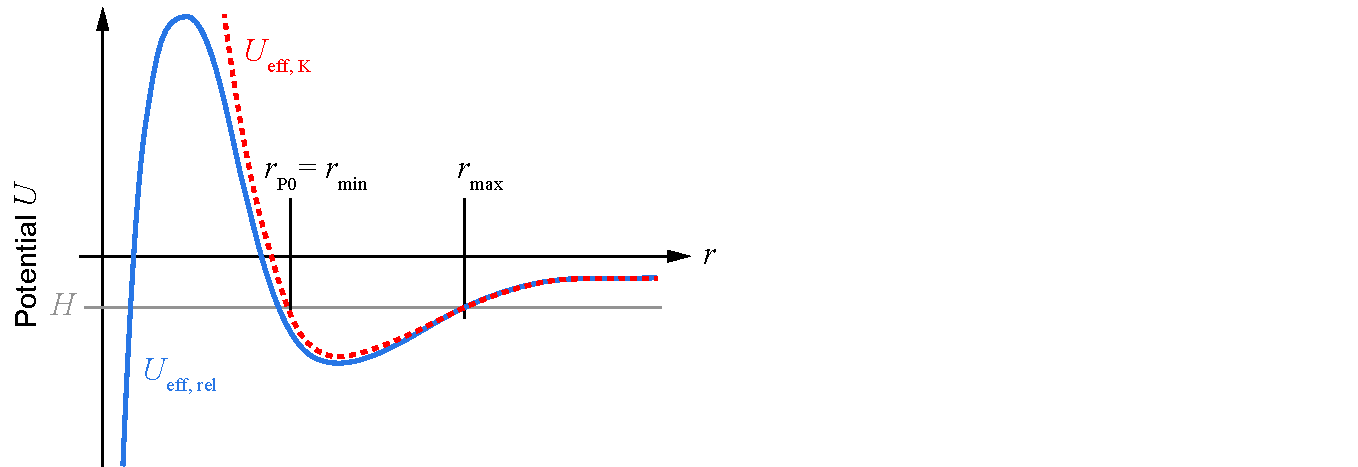
\includegraphics[width=\textwidth]{RelativisticPotential.pdf}%
\caption[Potential unter Ber�cksichtigung der relativistischen Korrektur.]{Darstellung des Potentials um einen Stern unter Ber�cksichtigung der relativistischen Korrektur, wobei $U_\text{eff,K}\!=\!-\mu_\text{G}/r + L^2/(2r^2)$ und $U_\text{eff,rel}\!=\!U_\text{eff,K}-\mu_\text{G}L^2/(c^2r^3)$. Die relativistische Korrektur ist im Bild stark �berh�ht dargestellt.}%
\label{abb:hm_relativistic_merkur}%
\end{figure} 
Wir wollen jetzt noch eine anschauliche Erkl�rung der relativistischen Perihelverschiebung geben.
Wir betrachten dazu \figref{hm_relativistic_merkur}, in der wir das effektive Potential ohne und mit stark �berh�hter relativistische Korrektur dargestellt haben.
Im nicht-relativistischen Fall ergibt das effektive Potential eine Senke, in der bei einer Energie $H\!<\!0$ der K�rper zwischen $r_\text{min}\!=\!r_{\text{P}_0}$ und $r_\text{max}$ seine Bahn hat.
Durch das relativistische Potential -- welches man sich als ein Ergebnis der Raumkr�mmung um die Zentralmasse herum vorstellen kann -- wird aber das effektive Potential bei kleinen $r$ (man beachte die $r^{-4}$-Abh�ngigkeit) so beeinflusst, dass der umlaufende K�rper bei gleicher Energie dem Zentralk�rper n�herkommt.
Da dort die Bahngeschwindigkeit am gr��ten ist, wird der Planet in gleicher Zeit einen etwas gr��eren Abschnitt der Bahn zur�cklegen.
Folglich hat er, wenn er zu seinem definierten Ausgangspunkt (\zb dem Perihel) zur�ckkommt, einen Winkel $>\! 2\pi$ �berstrichen.

In \probref{hm_perihel_kappa3} berechnen wir die Bahn f�r Potentiale mit beliebigem $\kappa_3$-Term.
Aus der Rechnung erh�lt man neben der schon abgesch�tzten Perihelverschiebung auch die zeitliche Entwicklung des Bahnradius als Funktion der wahren Anomalie $r(\upsilon(t))$.
Dieser zeigt durch das St�rpotential bedingt Oszillationen, wie wir sie bei der Betrachtung der Stabilit�t von Planetenbahnen bereits abgesch�tzt haben. F�r interessierte Leser sei auf eine sch�ne einfache linearisierte Berechnung der Merkurpr�zessions f�r den relativistischen Fall in Ref. \cite{Hall2022} verwiesen, die ebenfalls f�r ein nichtrelativistisches $\kappa_3/r^3$ St�rpotential verwendet werden kann.

\subsection{Kometen}\index{Kometen}\label{kap:kometen}
Kometen oder Schweifsterne sind faszinierende Himmelsk�rper.\footnote{Eine sehr lesenswerte und ausgesprochen ansprechend gestaltete �bersichten zu Kometen findet sich in \cite{Stump1988}.} Vermutlich sind sie nahezu unver�nderte Restmaterie aus der Entstehungszeit unseres Sonnensystems.
Die meisten Kometen werden aus ihren urspr�nglichen Bahnen durch Gravitationskr�fte und Kollisionen untereinander abgelenkt und auf langgestreckte Ellipsenbahnen geschickt.
Ein Komet besitzt einen Kern aus Staub und Eisk�rnern, der bei ausreichender Sonneneinstrahlung eine Gash�lle (Koma) und einen Schweif ausbildet.
Die L�nge des Schweifs kann mehrere hundert Millionen Kilometer erreichen.
Ber�hmte Kometen sind \zb der gro�e Komet von 1680, der am Tageshimmel zu sehen war, der Komet Donati von 1858, der als sch�nster Komet aller Zeiten gilt, und nat�rlich der ber�hmte Halleysche Komet.
Einigen Menschen ist es sogar verg�nnt, den Halleyschen Kometen\index{Halleyscher Komet}\index{Komet!Halleyscher} in ihrem Leben zweimal zu sehen.
Seine Ber�hmtheit erlangte er dadurch, dass seine Wiederkehr nach der Beobachtung im Jahr 1682 von Halley f�r 1758 vorhergesagt wurde.
Halley erlebte sie selbst nicht mehr.
Aber das von ihm vorhergesagte Wiedererscheinen des Kometen wurde am 25.12.1758 von dem s�chsischen Amateurastronomen(!) Palitzsch\footnote{Johann Georg Palitzsch (1723--1788) war ein s�chsischer Landwirt, Astronom und Naturwissenschaftler. Manche Literatur beschreibt ihn als \anf{Bauernastronom}, da er seine Beobachtungen auf seinem Landgut nahe bei Dresden machte.} tats�chlich beobachtet.
Dies war ein unglaublich gro�er und deutlich sichtbarer Erfolg der Newtonschen Gravitationstheorie\indexp{Newton, Sir Isaac}, der in etwa mit der Beobachtung der Lichtablenkung von 1919 zur Best�tigung der Allgemeinen Relativit�tstheorie verglichen werden kann.
Wir wollen uns im Folgenden auf wiederkehrende Kometen mit elliptischen Bahnen konzentrieren.
Die Berechnung elliptischer Kometenbahnen ist im Prinzip der f�r Planeten �hnlich.
Bei Kometen wird zur Bahnberechnung neben der Exzentrizit�t $e$ die \gls{periheldistanz} $q$ und der Periheldurchgang $t_0$ anstelle des Bahnradius und der mittleren Anomalie (Tabelle \ref{tab:hm_parameter_kometen}) angegeben.
Allerdings sind die Exzentrizit�ten bei Kometen sehr gro� ($e\!\approx\! 1$), was zu numerischen Schwierigkeiten bei der L�sung der Kepler-Gleichung f�hrt und die Benutzung der Mittelpunktsgleichung oder der einfachen Reihenentwicklungen nicht mehr erlaubt.
Wir werden deshalb zur Berechnung der exzentrischen Anomalie ein modifiziertes Verfahren benutzen (siehe \mscre \mlhmref{KometenZeit.m} und \mlhmref{KometenObsHor.m}).
Das Prinzip besteht darin, die Ellipsenbahn durch eine parabel�hnliche Bahn zu approximieren.
Wir  k�nnen dies hier nur skizzieren und verweisen f�r mehr Details auf die ausgezeichnete Darstellung in \cite{Montenbruck1999}.
F�r $e\!>\!0.9$ und eine mittlere Anomalie nahe am Perihel ($M\!<\!0.1\degree$) definiert man f�r diese Parabel-Approximation aus der exzentrischen Anomalie die sogenannten Stumpffschen\footnote{Karl Johann Nikolaus Stumpff (1895--1970) war ein deutscher Astronom, der in Berlin, Graz und G�ttingen vor allem auf dem Gebiet der mathematischen Himmelsmechanik forschte.} Funktionen\index{Stumpffsche Funktionen}\index{Funktionen!Stumpffsche}\cite{Walter2018}.
\begin{align}
c_1(E) &= \frac{\sin E}{E} = \sum_{n=1}^{\infty} (-1)^{n+1} \frac{E^{2(n-1)}}{(2n-1)!} \,, \label{eq:hm_Stumpff_fkt} \\
c_2(E) &= \frac{1-\cos E}{E^2} = \sum_{n=1}^{\infty} (-1)^{n+1} \frac{E^{2(n-1)}}{(2n)!} \,,\nonumber \\
c_3(E) &= \frac{E-\sin E}{E^3} = \sum_{n=1}^{\infty} (-1)^{n+1} \frac{E^{2(n-1)}}{(2n+1)!} \,. \nonumber
\end{align}
Man substituiert $E$ in der Kepler-Gleichung durch $c_3(E)$ und erh�lt mit \eqref{eq:hm_mittlere_anomalie}
\begin{equation*}
(1-e) E + e\,c_3(E)\, E^3 = \sqrt{\mu_\text{G} \lk \frac{1-e}{q} \rk^3} (t-t_0)  = M(t)  \,,
\end{equation*}
woraus mit der Hilfsgr��e 
\begin{equation*}
Q(e) = \sqrt{\frac{3\,e\, c_3(E)}{1-e}} E
\end{equation*}
aus der Kepler-Gleichung eine modifizierte Barker-Gleichung\index{Gleichung!Barker-} (siehe auch \probref{hm_bwglg_hyp_parab}) wird:
\begin{equation}
Q+\frac{Q^3}{3} = \sqrt{6\,e \, c_3(E)} \sqrt{\frac{\mu_\text{G}}{2q^3}}\,(t-t_0)\,.
\label{eq:hm_Barker_glg}
\end{equation}
Diese wird nun iterativ nach $E$ mit einem Anfangswert $E_0\!=\!0$ \bzw $c_3(0)\!=\!\frac{1}{6}$ gel�st.
Die so bestimmten exzentrischen Anomalien $E_n$ ($n$ wird bestimmt durch die Genauigkeit, die man erreichen will) werden dann zur Berechnung der Stumpffschen Funktionen\index{Funktion!Stumpffsche} $c_1(E_n), c_2(E_n), c_3(E_n)$ benutzt, wobei die Reihenformeln \eqref{eq:hm_Stumpff_fkt} sehr schnell konvergieren, was die gesamte Bahnberechnung damit schnell und relativ genau macht \cite{Montenbruck1999}.
Die Bahnkoordinaten ergeben sich zu
\begin{align}
x &= r\cos\upsilon = q \lk 1 - \frac{2\,c_2(E)}{6e\,c_3(E)} \,Q^2 \rk \,, \label{eq:hm_bahn_koord_komet} \\
y &= r\sin\upsilon = 2q \lk \frac{1+e}{2e} - \frac{1}{6\, c_3(E)}\, c_1(E) \, Q\rk \,, \nonumber \\
r &= q \lk 1+ \frac{2\,c_2(E)}{6\,c_3(E)}\,Q^2\rk \,.\nonumber
\end{align}
Die weitere Rechnung entspricht den Berechnungsschritten, wie wir sie bei den Planeten kennengelernt haben.
\figref{hm_kometenbahnen1} zeigt die Berechnungen f�r vier verschiedene Kometen.
Man beachte die starken Bahnneigungen zur Ekliptik und die parabelartigen Verl�ufe f�r Kometen mit gro�en Exzentrizit�ten.
Man erkennt auch sehr sch�n die Besonderheit des Halleyschen Kometen mit seiner f�r Kometen relativ kurzen Periode von $75.3$ Jahren und seiner retrograden\index{Bahn!retrograde} Bahn, die bis zu Neptun und Pluto reicht.

\begin{figure}%
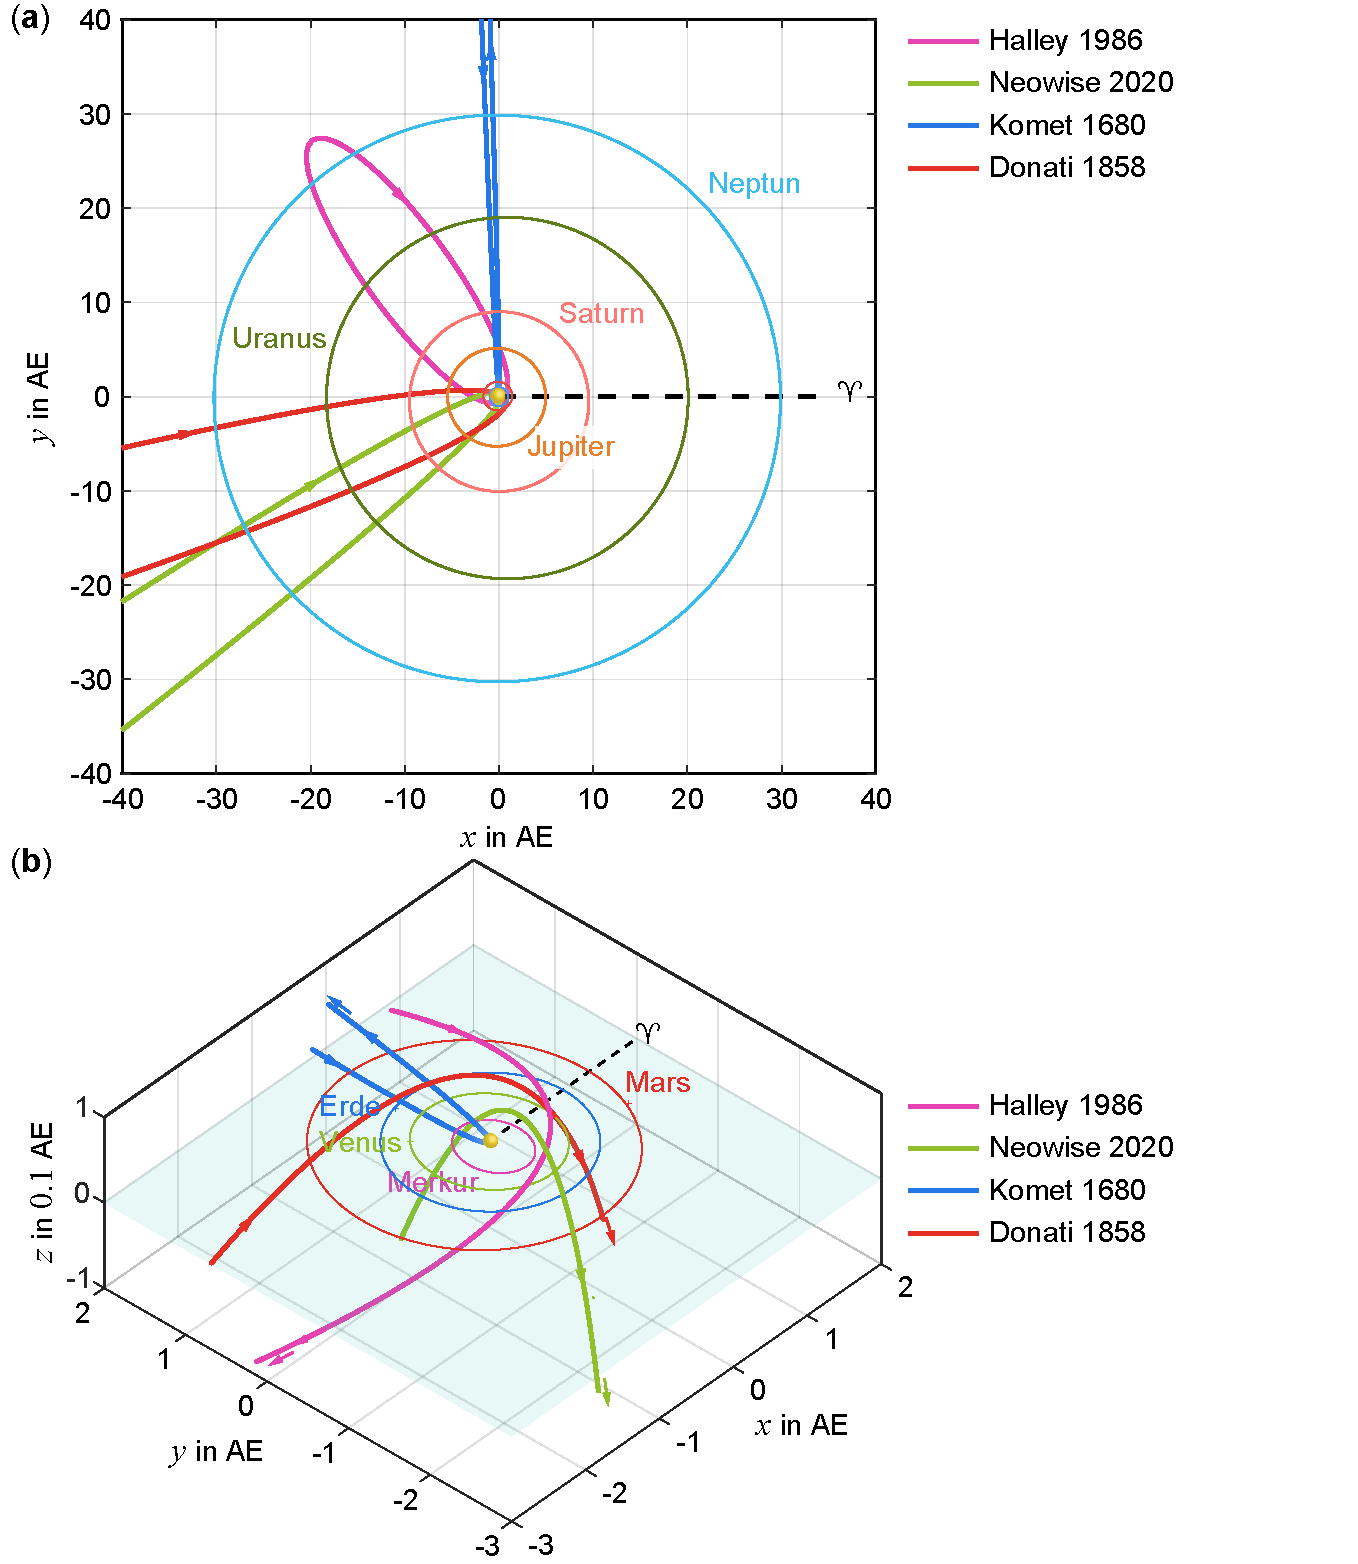
\includegraphics[width=\textwidth]{Komet1.pdf}%
\caption[Kometenbahnen im Vergleich.]{Bahnen verschiedener Kometen im Vergleich. \fa Projektion der Bahnen auf die Ekliptik. \fb 3D-Darstellung der Bahnen in Periheln�he (Sie \mscr~\mlhmref{KometenBahnen.m}).}%
\label{abb:hm_kometenbahnen1}%
\end{figure}

Wir m�chten an dieser Stelle aber noch auf einen Punkt hinweisen, der bei Berechnungen genaue Zeiten und Koordinaten f�r eine Beobachtung wichtig ist.
Bisher haben wir bei unseren Rechnungen die Lichtlaufzeit \index{Lichtlaufzeit} von den Planeten oder Kometen zum Beobachtungsort nicht ber�cksichtigt.
Die so berechneten Koordinaten hei�en deshalb auch astrometrische \index{Koordinaten!astrometrische} Koordinaten und entsprechen Beobachtungskoordinaten f�r eine angenommene Lichtgeschwindigkeit $c\rightarrow\infty$.
Bei fernen Kometen und auch Planeten ben�tigt das Licht aber f�r die Distanzen zu uns eine endliche Zeit $t_\text{L}\!\approx\!\Delta_0/c$.
W�hrend dieser Zeit bewegt sich der Himmelsk�rper weiter.
Der beobachtete Ort $\vec{r}_\text{B}$ liegt daher etwas \anf{hinter} dem Ort $\vec{r}_\text{HK}$, an dem sich der Himmelsk�rper zur Beobachtungszeit $t$ tats�chlich befindet, d.\,h. es gilt
\begin{equation}
\vec{r}_\text{B} = \vec{r}_\text{\astrosun}(t) + \lek \vec{r}_\text{HK}(t) - \dot{\vec{r}}_\text{HK}(t)\,t_\text{L}\rek \approx \vec{r}_\text{\astrosun}(t) + \lek \vec{r}_\text{HK}(t) - \dot{\vec{r}}_\text{HK}(t)\, \frac{\Delta_0}{c}\rek \,.
\label{eq:hm_scheinbare_koord_B}
\end{equation} 

Hierin sind $\vec{r}_\text{B}$ die beobachteten (scheinbaren) Koordinaten\index{Koordinaten!scheinbare}, $\vec{r}_\text{\astrosun}$ die geozentrischen Koordinaten der Sonne und $\vec{r}_\text{HK}$ die berechneten heliozentrischen (astrometrischen) Koordinaten des Himmelsk�rpers.
$\Delta_0$ ist die geometrische \gls{entfernunghimmelskoerper} und $\dot{\vec{r}}_\text{HK}$ die Bahngeschwindigkeit.
In \probref{hm_lichtlaufzeit} werden dazu einige Absch�tzungen angestellt, in \mlhmref{KometenBahnen.m} wird die im Allgemeinen kleine Korrektur bei der Berechnung der Beobachtungsdaten von Kometenbahnen ber�cksichtigt.
Bei nahen und relativ langsamen Objekten sind diese Korrekturen im Allgemeinen zu vernachl�ssigen. 
Da die Kometen auf ihrer Bahn viele St�rungen erfahren -- manchmal bleiben sie sogar unauffindbar --, unterscheiden sich die Bahnparameter von Periode zu Periode, wie man am Beispiel des  Halleyschen Kometen sehen kann, der seit einigen Jahrhunderten vermessen wird (\textbf{�bungen} \ref{prob:hm_kometen_asteroiden} und \ref{prob:hm_verweildauer_komet_erdbahn}). 

\begin{figure}%
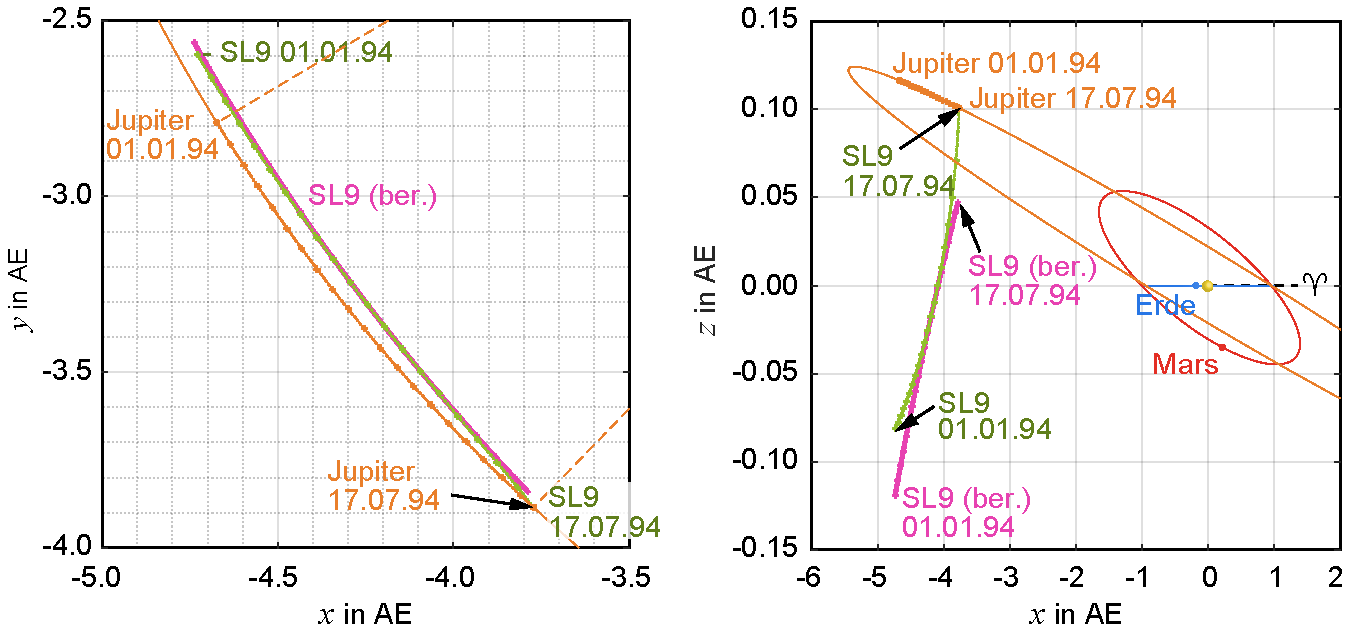
\includegraphics[width=\textwidth]{SL9.pdf}%
\caption[Shoemaker-Levy D/1993 F2.]{Shoemaker-Levy D/1993 F2 (Beispiel \ref{bsp:hm_shoemaker_levy}, \mlhmref{KometenSL9.m}). Man beachte, dass die rechte Abbildung in der $z$-Koordinate stark gestreckt ist!}%
\label{abb:hm_shoemaker_levy_komet}%
\end{figure}

Ein besonders beeindruckendes Beispiel einer Bahnver�nderung war der Komet Shoemaker-Levy.
Seine Bruchst�cke tauchten wie bereits erw�hnt im Juli 1994 in den Planeten Jupiter ein.
Wir haben bereits in \kapitel{stoerungsrechnung} die heliozentrischen Koordinaten dieses Kometen �ber numerische Integration bis zu seinem Zusammenprall mit Jupiter berechnet.
Wir vergleichen dieses Ergebnis mit der durch mittlere Bahnelemente gegebenen Keplerbahn.
Man erkennt in \figref{hm_shoemaker_levy_komet} sehr gut, dass die ungest�rte Kometenbahn durch die N�he zum Jupiter bereits 6 Monate vor dem Zusammensto� massiv beeinflusst wird.
Man kann also bereits zu diesem Zeitpunkt nicht mehr von einer ungest�rten Keplerbahn sprechen.\\
Im Juli 2020 hatten die Menschen auf der Nordhalbkugel der Erde das Gl�ck, den Kometen Neowise beobachten zu k�nnen.
Er bildete einen eindrucksvollen Schweif aus (\figref{hm_komet_neowise1}) und war mehrere Tage sehr gut nach Sonnenuntergang und vor Sonnenaufgang sichtbar.
Aus den in Tabelle \ref{tab:hm_parameter_kometen} angegebenen Werten k�nnen wir mit dem \mscr \mlhmref{KometenObsHor.m} dessen Bahn berechnen und auch erkennen, dass wir mit unserem Beobachtungsdatum gro�es Gl�ck hatten, da der Komet nur wenige Tage so gut sowohl am Abend- als auch am Morgenhimmel zu sehen war.
\begin{figure}%
\centering
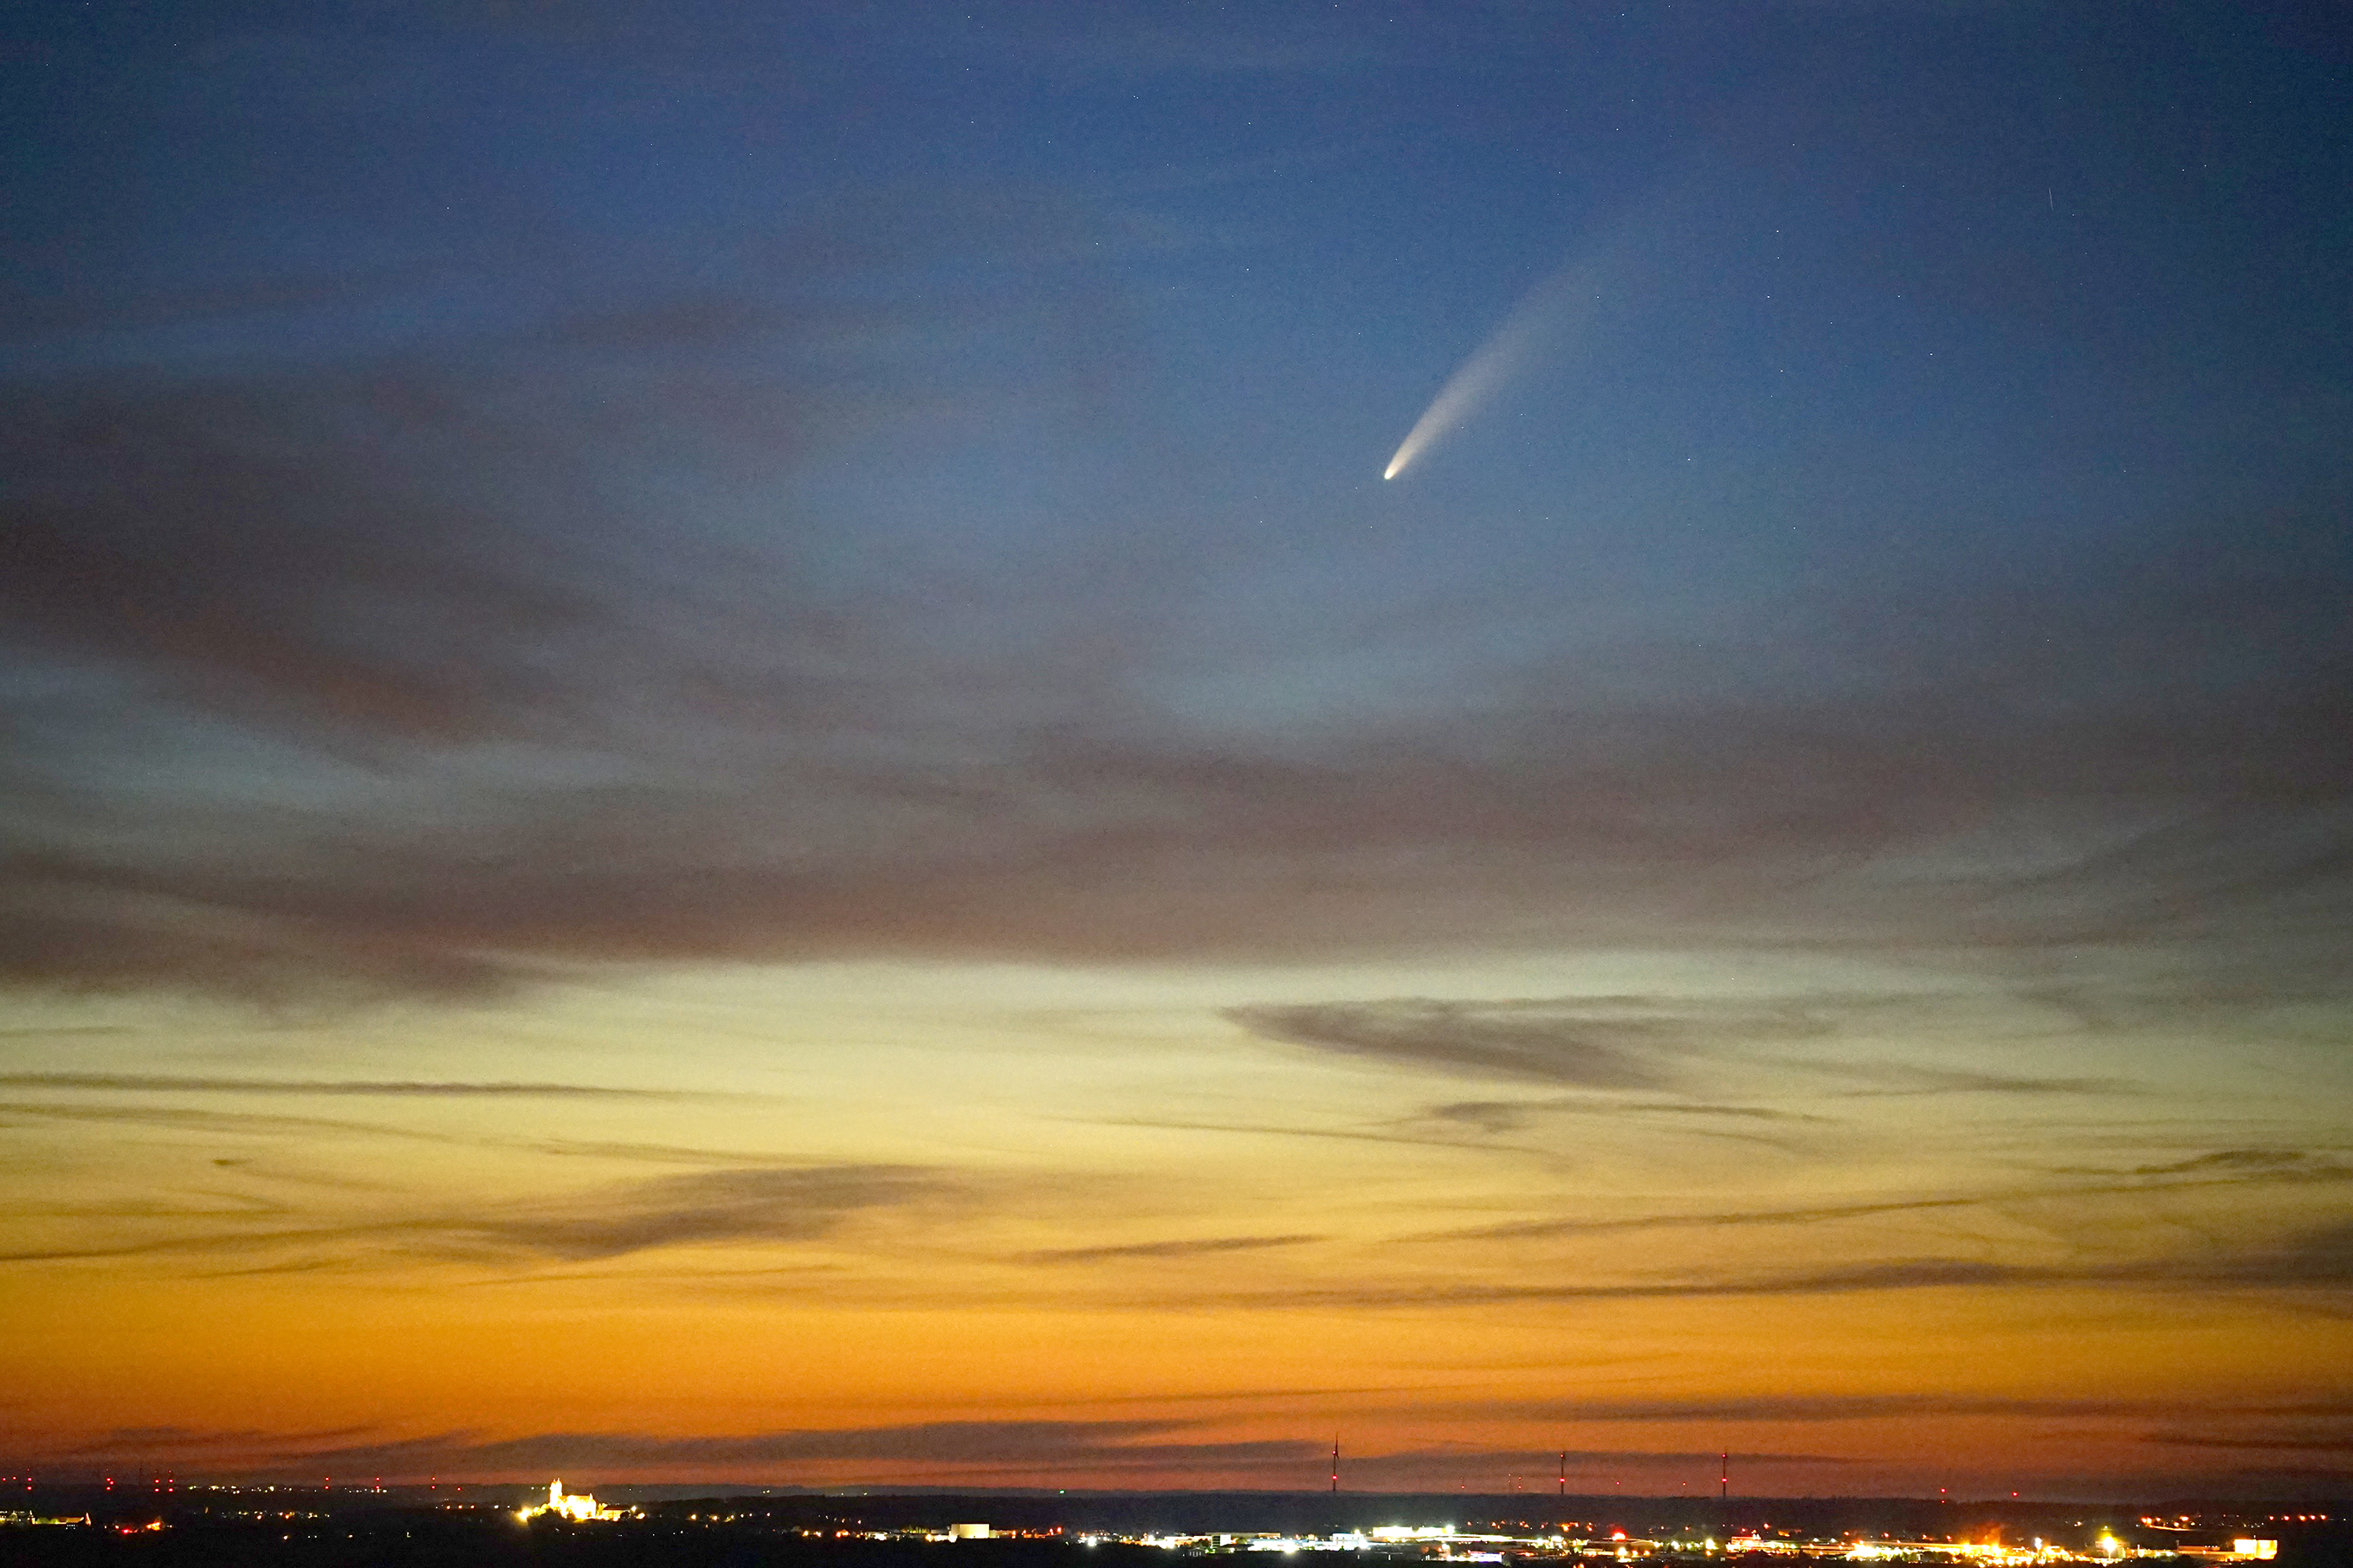
\includegraphics[width=0.75\textwidth]{KometNeowise.JPG} \\%
\caption[Beobachtung des Kometen Neowise von der Ostalb.]{Beobachtung des Kometen Neowise von der Ostalb aus ($48.8\degree$N, $10.2\degree$ O). Aufgenommen von Sylvia und Michael Kaschke am 12.07.2020, 22:30 MESZ.}%
\label{abb:hm_komet_neowise1}%
\end{figure}
\begin{figure}%
\centering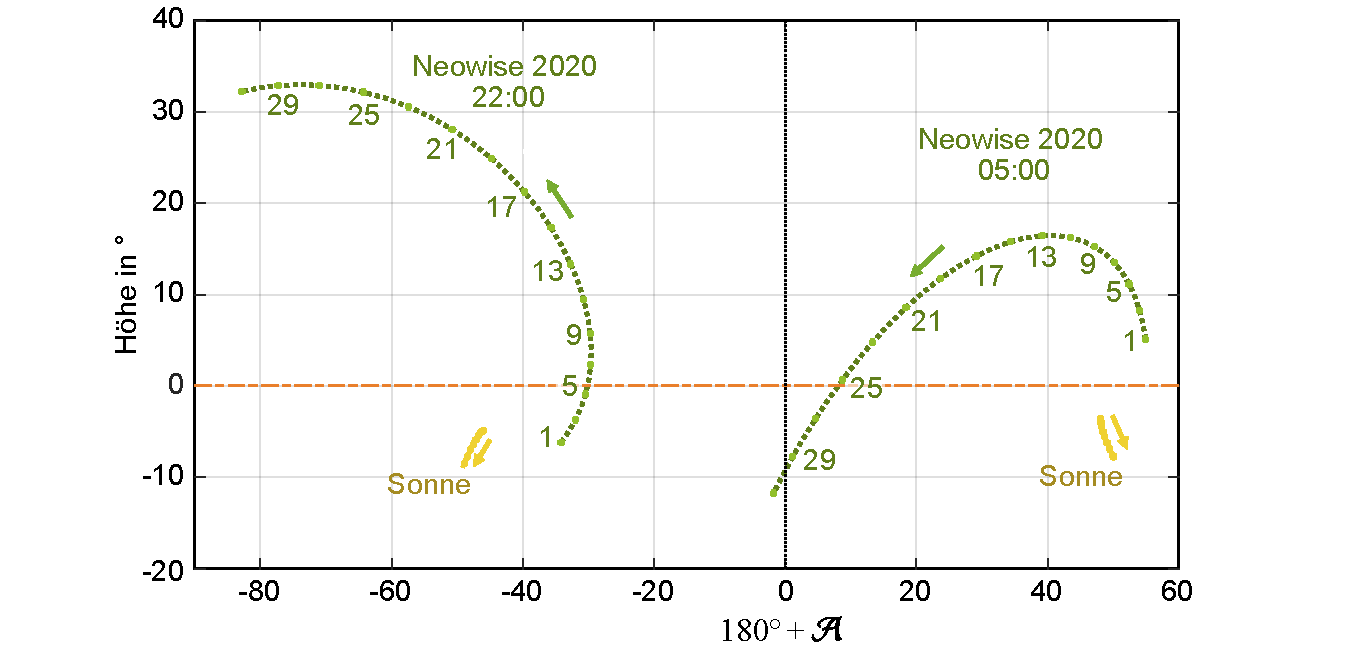
\includegraphics[width=\textwidth]{Neowise03.pdf}%
\caption{Berechnete Bahn des Kometen Neowise f�r den Monat Juli 2020.}%
\label{abb:hm_komet_neowise2}%
\end{figure}



\section{Berechnungen zu Sonnenfinsternissen}\label{kap:hm_sofis}\index{Sonnenfinsternis}\index{Mondfinsternis}

F�r Menschen ist eine totale Sonnenfinsternis (\figref{hm_Sofi2017})\footnote{Das Bild der totalen Sonnenfinsternis wurde mit einer Canon EOS700D und einem Celestron-Nexstar-5-Teleskop aufgenommen. Die Einzelbilder der partiellen Phasen wurden mit einer Canon 5D und einem 105-mm-Objektiv (M.~Kaschke, L.~Steger) fotografiert.} vermutlich mit eines der beeindruckendsten Ph�nomene, die man beobachten kann.
Die Kombination aus Seltenheit und K�rze einer solchen bogensekundengenau eintretenden Sonnenfinsternis (Englisch: \emph{Total Eclipse}), der abrupte Wechsel von Tag zu Nacht, das stundenlange Warten darauf und die oft tagelange Anreise in die h�ufig weit abgelegene Totalzone und nicht zuletzt das im Allgemeinen mit Jubel begr��te Wiedererscheinen der Sonne, all das macht das Erlebnis einer Sonnenfinsternis einzigartig und unvergesslich.
Wenn man bedenkt, dass bereits vor �ber 3000 Jahren Astronomen eine solche Sonnenfinsternis auf Minuten und wenige Kilometer genau vorhersagen konnten, kann man sich vorstellen, welche (nicht nur mentale) Macht diese Astronomen, die h�ufig auch die Hohepriester der herrschenden Dynastien waren, �ber die Menschen hatten.
Wir sind in der Lage, mit den in diesem Kapitel der Himmelsmechanik erarbeiteten Methoden und Kenntnissen diese Berechnungen selbst anzustellen.
Wir werden dabei nahezu das gesamte \anf{Handwerkszeug}, das wir in den vorausgehenden Kapiteln kennengelernt haben, anwenden k�nnen. 

\begin{figure}%
\centering\includegraphics[width=0.7\textwidth]{Sofi2017.jpg}%
\caption[Kompositaufnahme der Sonnenfinsternis 21.\,08.\,2017.]{Kompositaufnahme der Sonnenfinsternis 21.\,08.\,2017 am Snake River (Oregon/Idaho USA).} 
\label{abb:hm_Sofi2017}%Sofi2006
\end{figure}

\subsection{Mondbahn und Ekliptik -- Auftreten der Finsternisse}\label{kap:basics_sofis}

Wir beginnen zun�chst mit der Geometrie der Finsternisse.
Wiederum ist es bei der Betrachtung von Sonnen- und Mondfinsternissen vorteilhaft, in das geozentrische KOS zu wechseln.
Dazu werden wir das bereits in \kapitel{hm_naeherungsformeln_sonne} benutzte geozentrische Bild der \anf{scheinbaren} Bewegung der Sonne auf der Himmelssph�re (\figref{hm_wahre_sonne_geoz}) mit der Bahn des Erdmondes erg�nzen.
Dies ist in \figref{hm_Eclipse1} zu sehen.
Die Mondbahn hat eine Neigung von ca.$\:5\degree$ gegen�ber der Ekliptik und ihre Schnittpunkte mit der Ekliptik sind als \glslink{aufstknoten}{aufsteigender ($\ascnode$)}  \index{Knoten!aufsteigender} \bzw \glslink{abstknoten}{absteigender ($\descnode$) Knoten} \index{Knoten!absteigender} gekennzeichnet.

\begin{figure}%
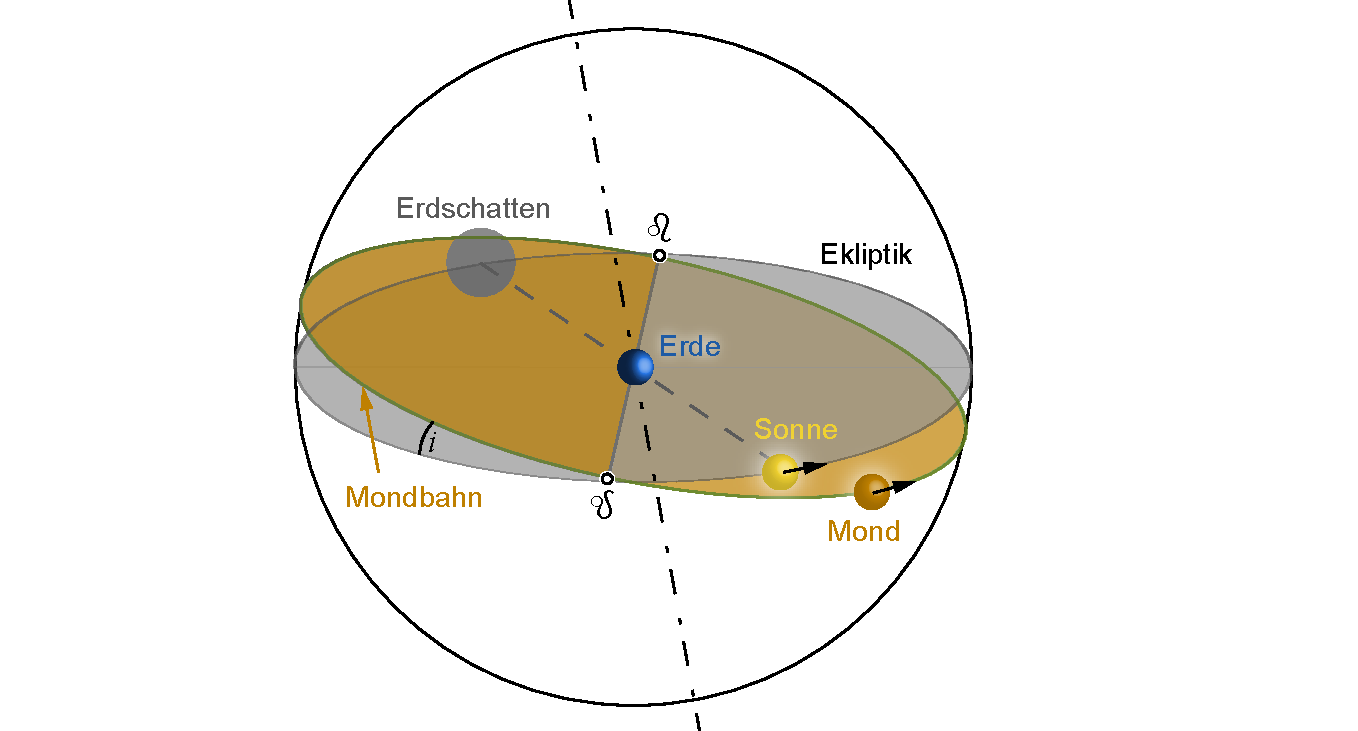
\includegraphics[width=\textwidth]{Eclipse1.pdf}%
\caption[Geozentrisches Bild der scheinbaren Bewegung von Sonne und Mond.]{Geozentrisches Bild der scheinbaren Bewegung von Sonne und Mond auf der Himmelssph�re.}%
\label{abb:hm_Eclipse1}%GeozentrGeometrie
\end{figure}

Da von der Erde aus betrachtet die scheinbaren Durchmesser\index{Durchmesser!scheinbarer} von Sonne und Mond einen etwa gleich gro�en Winkeldurchmesser von $0.5\degree$ haben, erscheinen beide Himmelsk�rper auch gleich gro� auf der Himmelssph�re.
Die Sonne \anf{durchl�uft} die Ekliptik einmal in einem tropischen Jahr.
Der Mond braucht f�r einen Bahnumlauf (z.\,B. von ${\ascnode}$ bis ${\ascnode}$) einen (siderischen) Monat.
Ebenfalls eingezeichnet ist der Schatten, den die Erdkugel auf die Himmelssph�re wirft.
Dieser hat in der Mondentfernung etwa einen Winkeldurchmesser von $1.4\degree$.
Man erkennt schon aus der Abbildung, dass Sonnen- und Mondfinsternisse nur in der N�he der Knoten stattfinden k�nnen, weil es sonst nicht zu einer Position der drei Himmelsk�rper kommt, in der sich die Schatten von Mond und Erde �berschneiden.
In \figref{hm_Eclipse2} haben wir solche m�glichen Konstellationen in der N�he des aufsteigenden Knotens $\ascnode$\glslink{aufstknoten}\ dargestellt. 
Wir betrachten zun�chst die Situationen bei Mondfinsternissen (\figref{hm_Eclipse2}a).
Offensichtlich gibt es eine Mondfinsternis nur bei Vollmond.
Die Sonne muss also (im Bild nicht dargestellt) in der N�he des absteigenden Knotens $\descnode$ der Mondbahn stehen: Der Erdschatten wandert durch den aufsteigenden Knoten $\ascnode$.
In der dargestellten Situation von Mond und Erdschatten\index{Erdschatten} kommt es dann zu einer partiellen Mondfinsternis.
Im Falle der Sonnenfinsternis stehen sowohl Sonne als auch Mond (und Mondschatten) in der N�he des Knotens.
Wir m�ssen uns daher von der Position des geozentrischen Beobachters l�sen und einen topozentrischen Beobachter auf der Erdkugel annehmen, da wegen der N�he des Mondes zur Erde dessen Parallaxe relativ gro� ist und nicht mehr vernachl�ssigt werden kann.
Folglich ist der Schattenbereich des Mondes, der von der Gesamtheit der Beobachter auf der Erdoberfl�che gesehen wird, gr��er als der Winkeldurchmesser des Mondes.
Mit anderen Worten: Die auf etwa $2\degree$ vergr��erten Schattenkreise enthalten alle Positionen der Mondoberfl�che, die von irgendeinem Punkt auf der Erdoberfl�che gesehen werden k�nnen.
Bei einer �berdeckung eines solchen Mondschattenkreises mit der Sonne, wie in der Situation in \figref{hm_Eclipse2}b dargestellt, kommt es zu einer (partiellen) Sonnenfinsternis.
Diese ist dann f�r bestimmte Punkte auf der Erdoberfl�che sichtbar.

\begin{figure}%
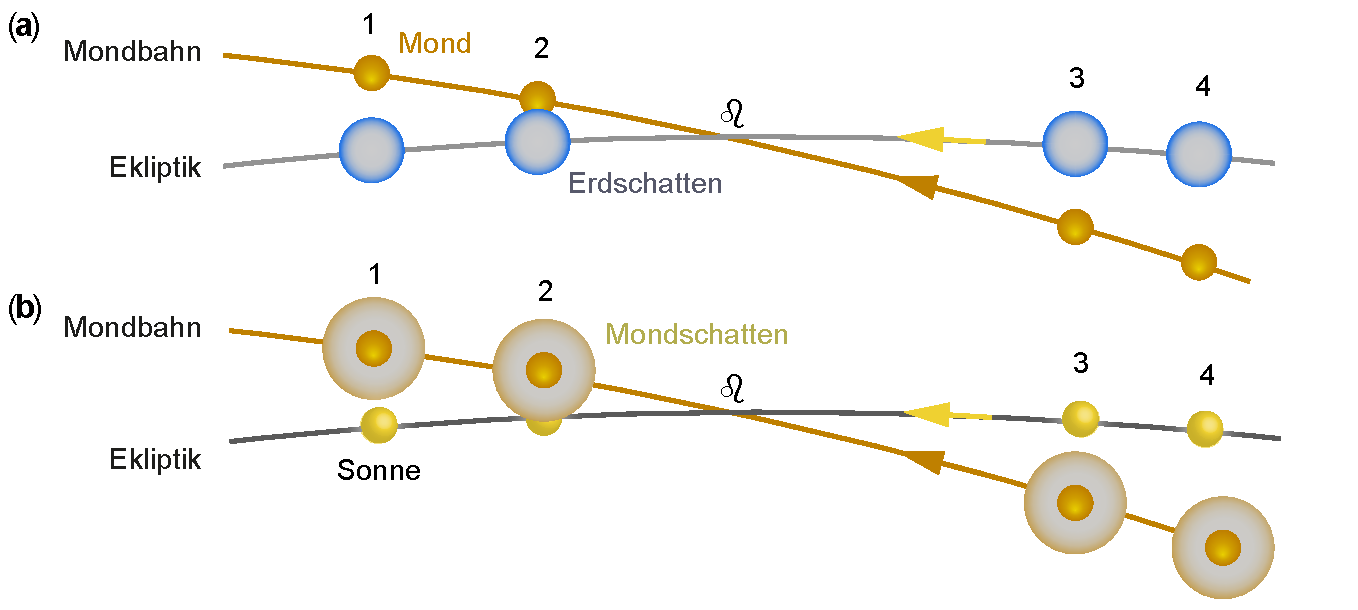
\includegraphics[width=\textwidth]{Eclipse2.pdf}%
\caption[Mond, Sonne und Schattenpositionen einer m�glichen Finsternis.]{Mond, Sonne und Schattenpositionen einer m�glichen Mondfinsternis. \fa Mondfinsternis (MF) und \fb Sonnenfinsternis (SF) am aufsteigenden Knoten der Mondbahn.}%
\label{abb:hm_Eclipse2}%AufsteigenederKnoten
\end{figure}

Mit diesem Verst�ndnis ist es nun m�glich, die Zeiten f�r eine m�gliche Sonnenfinsternis (oder Mondfinsternis) zu berechnen.
Wir m�ssen die Neumondzeitpunkte f�r Sonnenfinsternisse bzw. Vollmondzeitpunkte f�r Mondfinsternisse berechnen und die zu diesen Zeiten vorliegende ekliptikale geozentrische Breite des Neumondes $\beta_{\newmoon}$ bzw. Vollmondes $\beta_{\fullmoon}$ bestimmen.\footnote{Wir wollen uns im Folgenden auf die Sonnenfinsternis konzentrieren.
Alle Herleitungen gelten v�llig analog auch f�r die Mondfinsternis (siehe auch \probref{hm_MoFi}).}

Am einfachsten bestimmt man die Neumondzeiten, indem man die Funktion $\Delta \lambda (t)$ als Differenz der geozentrisch-ekliptikalen L�ngen von Sonne und Mond bildet,
\begin{equation}
  \Delta \lambda (t) = \lambda_\text{\astrosun} (t) - \lambda_\text{M} (t) \; ,
  \label{eq:hm_newmoon_determ}
\end{equation}
und die Nullstellen dieser Funktion ermittelt.\footnote{Nochmaliger Hinweis: Bei der Berechnung der Finsternis-Koordinaten ist darauf zu achten, dass man die Ephemeridenzeit ET benutzt und die Lichtlaufzeit von der Sonne zur Erde ber�cksichtigt.}
F�r die geozentrischen Koordinaten von Mond und Sonne haben wir in den \mscren entsprechende Routinen hinterlegt, die auch die relativ genauen analytischen Reihenentwicklungen f�r die Mond- und Sonnenbahn (siehe \kapitel{stoerungsrechnung}) verwenden.
Ein Berechnungsbeispiel f�r die Neumondzeiten �ber einen Zeitraum von 100 Jahren ist in \probref{hm_MoFi} zu finden.

\subsection{Schattengr��en und Orte einer totalen Sonnenfinsternis}
In \figref{hm_Eclipse3} haben wir die Schattenkegel\index{Schattenkegel}\index{Schattengr��e} eingezeichnet, die der Mond (hier auf die Erde) wirft.
Man erkennt einen \gls{ks}bereich\index{Kernschatten} (KS) und zwei Halbschattenbereiche\index{Halbschatten} (HS).
Je nach Abstand zwischen Erde und Mond kann es dann im KS-Bereich zur Ausbildung einer \glslink{tf}{totalen Finsternis}\index{Sonnenfinsternis!totale} (TF) oder einer \glslink{rf}{ringf�rmigen Finsternis}\index{Sonnenfinsternis!ringf�rmige} (RF) kommen.
Wir wollen den Durchmesser des Schattenkegels auf der Erdoberfl�che berechnen.
Aus \figref{hm_Eclipse4} k�nnen wir die geometrische Beziehung ableiten.
Wir starten mit
\begin{align*}
	q\sin\eta &= R_\text{M} ~~\text{und}\\
	(q + r_\text{\astrosun M})\,\sin\eta &= R_\text{\astrosun}\,.
\end{align*}
Daraus folgt sofort
\begin{align}
	\sin\eta &= \frac{R_\text{\astrosun} - R_\text{M}}{r_\text{\astrosun M}} ~~\text{und} ~~ 
	q = \frac{R_\text{M}\, r_\text{\astrosun M}}{R_\text{\astrosun} - R_\text{M}} \,.\label{eq:hm_sofi_basic01}
\end{align}

\begin{figure}%
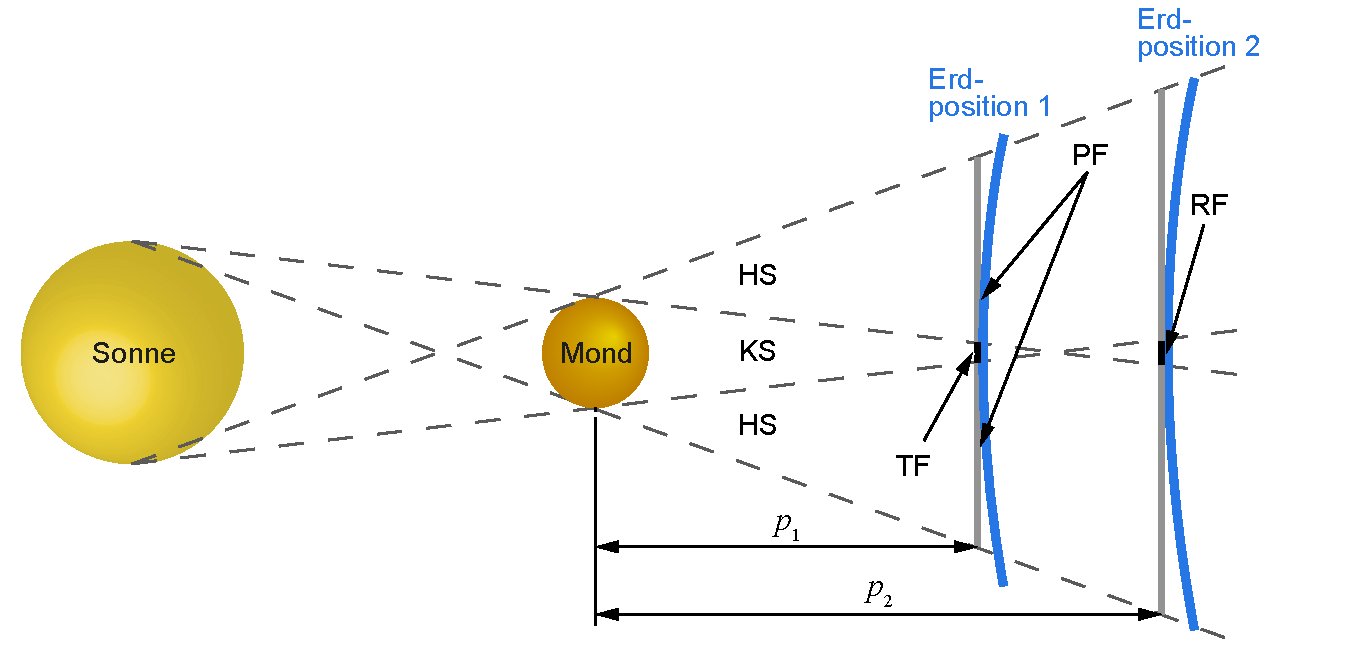
\includegraphics[width=\textwidth]{Eclipse3.pdf}%
\caption[Geometrie von Kern- und Halbschatten.]{Geometrie von Kern- und Halbschatten, sowie von totaler (TF), partieller (PF) und ringf�rmiger (RF) Sonnenfinsternis (Zur besseren Anschaulichkeit nicht ma�st�blich und auch nicht in den korrekten Proportionen gezeichnet!)}%
\label{abb:hm_Eclipse3}%Schatten- und Finsternisarten
\end{figure} 

\begin{figure}%
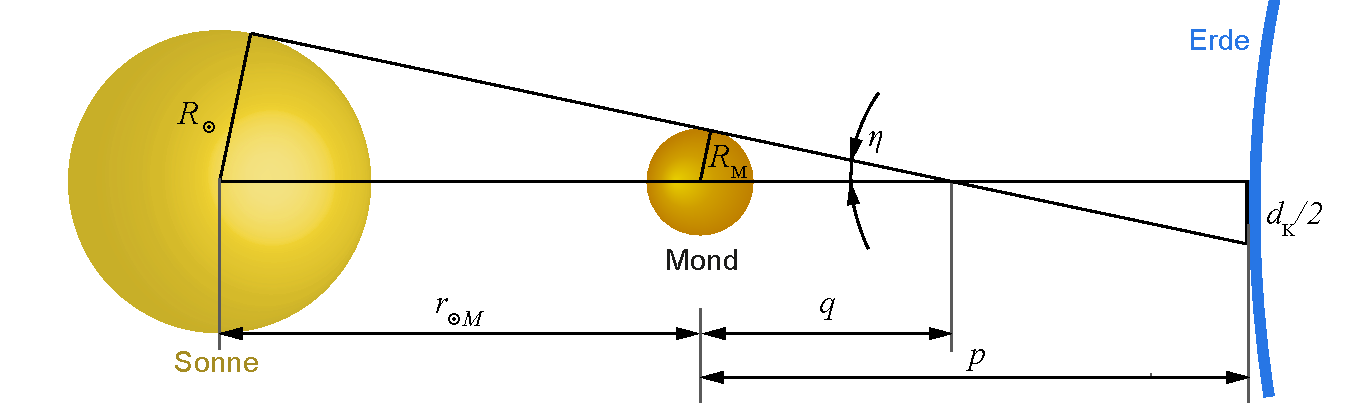
\includegraphics[width=\textwidth]{Eclipse4.pdf}%
\caption{Schattendurchmesser einer totalen Sonnenfinsternis.}%
\label{abb:hm_Eclipse4}%Schattendurchmesser
\end{figure}

Ferner k�nnen wir aus \figref{hm_Eclipse4} ablesen:
\begin{equation*}
\frac{d_\text{K}}{2} = (p-q)\,\tan\eta \,.
\end{equation*}
Mit der N�herung f�r kleine Winkel $\tan\eta\!\approx\!\sin\eta$ erh�lt man schlie�lich unter Nutzung von \eqref{eq:hm_sofi_basic01} f�r den Kernschattendurchmesser
\begin{align}
\frac{d_\text{K}}{2} &= \frac{p\,R_\text{\astrosun}}{r_\text{\astrosun M}} - \lk 1+\frac{p}{r_\text{\astrosun M}} \rk R_\text{M} ~ \nonumber\\
\rightarrow d_\text{K}(p) &= 2R_\text{\astrosun}\lk \frac{p}{r_\text{\astrosun M}} \rk - 2 R_\text{M} \lk 1+\frac{p}{r_\text{\astrosun M}}\rk \,. \label{eq:hm_schattenkegel1}
\end{align}
Setzt man die Werte $2R_\text{\astrosun}\!=\! 218.4 R_\text{\earth}$ und $2R_\text{M}\!=\! 0.545 R_\text{\earth}$ ein und nimmt in guter N�herung $r_\text{\astrosun M}\!\approx\! 1\:\text{AE} - 380000\:\text{km}\pm 25000\:\text{km}$ an, dann findet man f�r den Kernschattendurchmesser Werte zwischen $250$ und $350\:$km.
Das hei�t, dass nur ein kleiner Teil der Erdoberfl�che vom Kernschatten getroffen wird, was die oft langen Reisen zu den Finsternisorten erkl�rt.
Entsprechend gilt f�r den Halbschattendurchmesser
\begin{align}
D_\text{H}(p) &= 2R_\text{\astrosun}\lk \frac{p}{r_\text{\astrosun M}} \rk + 2 R_\text{M} \lk 1+\frac{p}{r_\text{\astrosun M}}\rk \,. \label{eq:hm_schattenkegel2}
\end{align}

\begin{figure}%
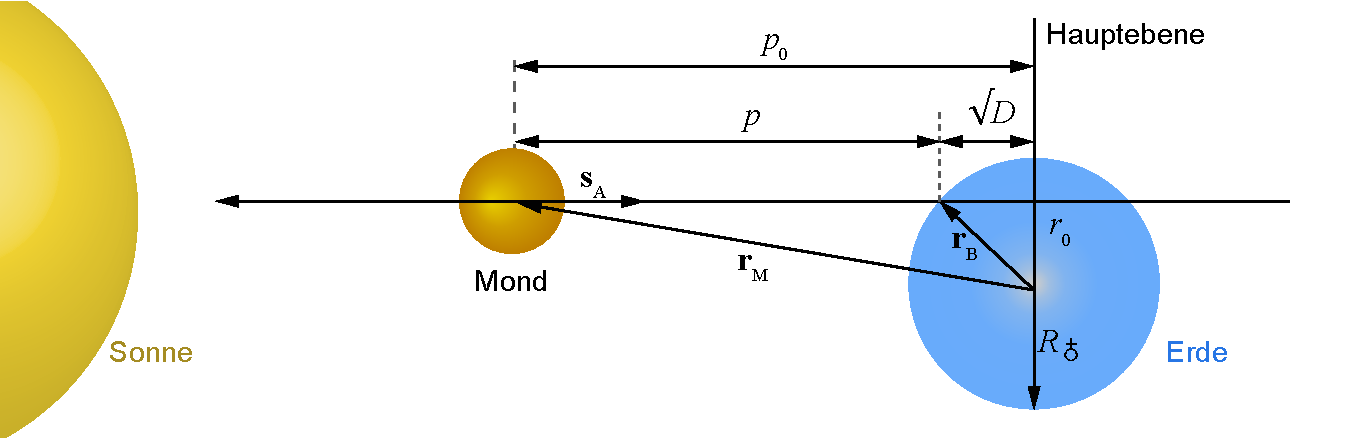
\includegraphics[width=\textwidth]{Eclipse5.pdf}%
\caption[Auftreffpunkt der Kernschattenachse auf der Erdoberfl�che.]{Berechnung des Auftreffpunktes der Kernschattenachse auf der Erdoberfl�che.}%
\label{abb:hm_Eclipse5}%Schnittpunkt Schattenachse
\end{figure}
Den Ort des Auftreffens der Achse des KS-Kegels ermitteln wir mit Hilfe von \figref{hm_Eclipse5}.
Die Achse $\vec{s}_\text{A}$ wird durch die Richtung von der Sonnenmitte zur Mondmitte definiert und kann andererseits als
\begin{equation}
\vec{s}_\text{A} = \frac{\vec{r}_\text{B} - \vec{r}_\text{M}}{\abs{\vec{r}_\text{B} - \vec{r}_\text{M}}} ~\label{eq:hm_achse_ks_kegel}
\end{equation}
beschrieben werden.
Hierin sind $\vec{r}_\text{M}$ der geozentrische Ortsvektor des Mondes und $\vec{r}_\text{B}$ der Vektor des Auftreffpunktes der Schattenachse auf der Erdoberfl�che, also dort, wo sich ein Beobachter einer TF idealerweise befinden sollte.
Aus \figref{hm_Eclipse5} lesen wir ferner ab, dass
\begin{align}
	\vec{r}_\text{B} &= \vec{r}_\text{M} + p\,\vec{s}_\text{A} = \lk \begin{matrix} x_\text{M} + p \,s_{\text{A},x} \\ y_\text{M} + p \,s_{\text{A},y} \\z_\text{M} + p \,s_{\text{A},z}\end{matrix}\rk\, = \,\lk \begin{matrix} x_\text{B} \\ y_\text{B} \\ z_\text{B} \end{matrix} \rk \,, \label{eq:hm_auftreffvek}\\
	\vec{r}_\text{B}^2 &= x_\text{B}^2 + y_\text{B}^2 + z_\text{B}^2 = R_\text{\earth}^2 \,. \label{eq:hm_auftreffvek2}
\end{align}
In \eqref{eq:hm_auftreffvek2} haben wir zun�chst noch die Kugelgestalt der Erde angenommen.
Setzt man nun \eqref{eq:hm_auftreffvek} in \eqref{eq:hm_auftreffvek2} ein, ergibt sich
\begin{equation*}
p^2 + 2p \,\vec{r}_\text{M}\,\vec{s}_\text{A} + (r_\text{M}^2 - R_\text{\earth}^2) = 0
\end{equation*}
mit den L�sungen
\begin{equation}
p = p_0 \pm \sqrt{D} \,,\label{eq:hm_lsg_p}
\end{equation}
worin $p_0$ und $D$ durch
\begin{align*}
	p_0 &= - \lk x_\text{M} e_x + y_\text{M} e_y + z_\text{M} e_z\rk ~~\text{\bzw} ~~	D = p_0^2 + R_\text{\earth}^2 - r_\text{M}^2 \,
\end{align*}
gegeben sind. Physikalisch sinnvoll ist nur die L�sung mit dem negativen Vorzeichen, da diese einen Punkt auf der Tagseite der Erde beschreibt.
Die L�sung $p = p_0 + \sqrt{D}$ beschreibt einen Punkt auf der Nachtseite der Erde.
Falls $D\!<\!0$, l�uft die Schattenachse an der Erde vorbei und es kommt zu keiner Finsternis.
Damit haben wir den \anf{Zentralort} der totalen Finsternis auf der Erdoberfl�che bestimmt:
\begin{equation}
\vec{r}_\text{B} = \vec{r}_\text{M} + (p_0 - \sqrt{D}) \,\vec{s}_\text{A} \,. \label{eq:hm_zentralort_tot_finsternis}
\end{equation} 
Damit eine totale Sonnenfinsternis auftreten kann, muss gem�� \figref{hm_Eclipse5} noch gelten, dass
\begin{equation*}
r_\text{M}^2 - p_0^2 < R_\text{\earth}^2 \,.
\end{equation*}
Bisher haben wir die Erde als perfekte Kugel betrachtet.
Jetzt m�ssen wir deren Abplattung ber�cksichtigen.
Die Erde kann als Rotationsellipsoid mit einem um $(1-f) = 0.996647$ gestauchten Polarradius gegen�ber dem mittleren Radius $R_\text{\earth}$ angenommen werden.
Die bisherigen Rechnungen kann man gl�cklicherweise einfach weiter verwenden, indem man in \eqref{eq:hm_auftreffvek2} die $z$-Koordinate der Beobachterkoordinaten um den Betrag der Abplattung $(1-f)$ staucht. \eqref{eq:hm_auftreffvek2} lautet dann
\begin{align}
		\vec{r}_\text{B}^2 &= x_\text{B}^2 + y_\text{B}^2 + z_\text{B}^2 \, (1-f)^2 = R_\text{\earth}^2 \,. \label{eq:hm_auftreffvek3}
\end{align}
Alle anderen Berechnungsschritte bleiben wie oben dargestellt.

\subsection{Ber�cksichtigung der Abplattung der Erde}
Wir m�ssen zur Ortsbestimmung der Finsternis noch die Rotation der Erde ber�cksichtigen.
Ohne Abplattung der Erde w�re das relativ einfach, weil wir aus den geozentrischen Koordinaten des Mondes �ber die Deklination direkt die Breite des Beobachtungspunktes erhielten und aus der Rektaszension des Mondes �ber die Sternzeit auch die geographische L�nge berechnen k�nnten.
Durch die Abplattung der Erde ist aber die geographische Breite nicht gleich der geozentrischen Breite (die wiederum der Deklination entspricht).
F�r die Umrechnung \glslink{geozentrkoord} von geozentrischen $(\varphi_\text{B}',\,\lambda'_\text{B})$ in geographische\index{Koordinaten!geographische} Koordinaten $(\varphi_\text{B},\,\lambda_\text{B})$ eines Beobachtungspunktes auf der Erde besteht in guter N�herung der Zusammenhang \cite{Montenbruck1999}:
\begin{align}
\varphi &= \varphi' + 0.1924\degree\,\sin(2\varphi')\; , \qquad ~~\lambda = \lambda'\,. \label{eq:hm_umrechnung_geogr_geozent_Koord}
\end{align}
Die geographische L�nge kann �ber die bekannte Beziehung \eqref{eq:hm_LMST} mittels der Sternzeit $\theta(t)$ aus der Rektaszension berechnet werden (siehe \kapitel{hm_raum_und_zeit}):
\begin{equation}
\alpha = \theta_0(t) + \lambda\,a\,e \; .\label{eq:hm_geogr_laenge_rektaszension}
\end{equation}
Damit kann der Ortsvektor des Auftreffpunktes der Schattenachse auf der Erdoberfl�che geschrieben werden als
\begin{align}
\lk \begin{matrix} x_\text{B} \\ y_\text{B} \\ z_\text{B} \end{matrix}\rk &= \lk \begin{matrix} r_\text{B}\cos\varphi' \cos\lambda \\ r_\text{B}\cos\varphi' \sin\lambda \\ r_\text{B}\sin\varphi' \end{matrix}\rk = \mathbb{R}_z\lk\theta(t)\rk\,\lk \begin{matrix} r_\text{B}\cos\delta \cos\alpha \\ r_\text{B}\cos\delta \sin\alpha \\ r_\text{B}\sin\delta \end{matrix}\rk \,. \label{eq:hm_schattenachse_auf_erde}
\end{align}
Zur Erinnerung $x_\text{B}, y_\text{B}, z_\text{B}, r_\text{B}$ sind bekannt \bzw berechnet, bestimmt werden aus \eqref{eq:hm_schattenachse_auf_erde} $\lambda, \varphi'$.
Ebenfalls sei nochmals der Hinweis gegeben, dass die Koordinatenberechnung $(\alpha,\,\delta)$ immer mit der ET zu erfolgen hat.
F�r die Berechnung der Sternzeit brauchen wir aber nach Gleichung \eqref{eq:hm_UT_3} die UT.
Zwischen beiden Zeiten besteht ein Unterschied $\Delta T$.
Man muss diesen also f�r den Zeitraum der Finsternis kennen oder zumindest �ber N�herungs-Polynome \cite{Espenak2014} absch�tzen k�nnen.
Mit \eqref{eq:hm_schattenachse_auf_erde} k�nnen wir nun den geographischen Ort $(\varphi(\varphi'=\delta),\,\lambda(\alpha))$ zur Zeit des Auftretens des Schattenkegels der Sonnenfinsternis berechnen.
Die Linie entlang aller geographischen Orte, die so zu den verschiedenen Zeitpunkten der maximalen Finsternis berechnet werden, wird Zentrallinie genannt. 

\subsection{Finsternisdauer}\index{Sonnenfinsternis!Dauer}
Mit den Beziehungen \eqref{eq:hm_lsg_p} und \eqref{eq:hm_zentralort_tot_finsternis} lassen sich zu dem mittels \eqref{eq:hm_newmoon_determ} ermittelten Finsterniszeitpunkt $t_0$ die kartesischen Koordinaten des Schattenkegels zu
\begin{align}
\vec{r}_\text{B0}(t_0) &= \lk \begin{matrix} x_\text{B0}(t_0) \\ y_\text{B0}(t_0) \\ z_\text{B0}(t_0)\end{matrix} \rk
\label{eq:hm_schatten_kartes_1}
\end{align}
und zu einem etwas sp�teren Zeitpunkt $t_1\!=\!t_0+\Delta t$ zu
\begin{align}
\vec{r}_\text{B1}(t_1) &= \lk \begin{matrix} x_\text{B1}(t_1) \\ y_\text{B1}(t_1) \\ z_\text{B1}(t_1)\end{matrix} \rk \label{eq:hm_schatten_kartes_2}
\end{align}
berechnen.
$(\vec{r}_\text{B1} - \vec{r}_\text{B0})/\Delta t$ ist dann ein Ma� f�r die Geschwindigkeit, mit der sich der Kernschatten fortbewegt.
Um aber die Bewegung des Schattens relativ zur Erdoberfl�che zu berechnen, muss man noch die Rotation der Erde ber�cksichtigen, denn in der Zeit $\Delta t$ dreht sich die Erde um einen Winkel
\begin{equation}
\xi = \frac{2\pi\!\Delta t}{d_\diamond} \,. \label{eq:hm_winkeldrehung_erde}
\end{equation}
Hierin ist $d_\diamond$ die Dauer eines Sterntages. In der Zeitspanne $\Delta t$ haben sich also die �quatorialen Koordinaten des Punktes $\vec{r}_\text{B1}(t_0+\Delta t)$ durch Drehung so ver�ndert, dass dieser Punkt zur Zeit $t_0$ die Koordinate
\begin{equation}
\vec{r}'_\text{B1} (t_0) = \mathbb{R}_z(\xi)\,\vec{r}_\text{B1}(t_1) ~ \label{eq:hm_koord_nach_winkeldrehung}
\end{equation}
hat.
Der Kernschatten legt folglich im Zeitraum $\Delta t$ bezogen auf das \emph{earth-fixed} KOS (siehe \kapitel{hm_koordinatensysteme}) den Weg $\Delta\vec{r}\!=\!\vec{r}'_\text{B1}-\vec{r}_\text{B0}$ zur�ck.
Da $\Delta t$ eine kurze Zeit ist, kann man die Rotationsmatrix $\mathbb{R}_z(\xi)$ f�r kleine Winkel $\xi$ vereinfachen und n�herungsweise schreiben:

\begin{equation*}
\Delta\vec{r} = \lk \begin{matrix} \Delta x \\ \Delta y \\ \Delta z \end{matrix}\rk  = \lk \begin{matrix} x'_\text{B1} \\ y'_\text{B1} \\ z'_\text{B1} \end{matrix}\rk - \lk \begin{matrix} x_\text{B0}\\ y_\text{B0} \\ z_\text{B0} \end{matrix}\rk = \lk \begin{matrix} x_\text{B1} + \xi y_\text{B1} - x_\text{B0} \\ y_\text{B1} - \xi x_\text{B1} - y_\text{B0} \\ z_\text{B1} - z_\text{B0} \end{matrix}\rk\,\,.
\end{equation*}


Unter Benutzung von \figref{hm_Eclipse5} zerlegt man $\Delta\vec{r}$ in einen Anteil parallel zu $\vec{e}$ und einen Anteil senkrecht zu $\vec{e}$:
\begin{align*}
	\Delta r_\parallel &= \Delta\vec{r}\cdot\vec{e} = \Delta x\,e_x + \Delta y\, e_y + \Delta z\, e_z ~~\text{und} \\
	\Delta r_\perp &= \sqrt{\Delta r^2 - \Delta r_\parallel^2} \,.
\end{align*}
Die tats�chliche, effektive Geschwindigkeit, mit der sich der Kernschatten senkrecht zur Einfallrichtung des Schattenkegels weiterbewegt, ist $v_\perp\!=\!\Delta r_\perp / \Delta t$.
Die Dauer der totalen Finsternis an einem Punkt ist dann gegeben durch
\begin{equation}
t_z = \frac{\abs{d}}{v_\perp}\,, \label{eq:hm_dauer_kernschatten}
\end{equation}
worin $d$ der nach \eqref{eq:hm_schattenkegel1} berechnete Durchmesser des Kernschattens zur jeweiligen Zeit ist.

Wir haben damit alle Berechnungsformeln, um den Zeitpunkt, den geographischen Ort (inkl.\ Breite der Totalit�tszone) und die Dauer der Totalit�t zu berechnen.

\subsection{Zusammenfassende Darstellung des Algorithmus in \matlab}
Wir gehen im Folgenden noch einmal zusammenfassend die Einzelschritte zur Berechnung der Daten f�r eine totale Sonnenfinsternis an, wie diese auch in den \mscren \mlhmref{Sonnenfinsternis01.m}, \mlhmref{Sonnenfinsternis02.m} und \mlhmref{Sonnenfinsternis03.m} hinterlegt sind.
Wir folgen hierbei der exzellenten Darstellung des Themas in \cite{Montenbruck1999}, haben diese aber auf die Berechnungen in \matlab{} angepasst. 

\begin{enumerate}[1.]
  \item Mit Hilfe der \mscre \mlhmiref{SonneExakt.m} und \mlhmiref{MondExakt.m}  berechnen wir die geozentrisch-ekliptikalen Koordinaten von Sonne und Mond und untersuchen die Funktion $\Delta \lambda (t)\!=\!\lambda_\text{\astrosun} (t)\!-\!\lambda_\text{M} (t)$ �ber einen bestimmten Zeitraum hinweg auf Nullstellen.
          Dabei ist als Zeit ET zu nehmen.
          F�r die Sonne m�ssen wir wegen der Lichtlaufzeit $\tau_\text{\,L}\!=\!8.32 \:\text{min}$ die Zeiten entsprechend zur�ckversetzt berechnen.
	\item Gibt es eine Nullstelle $t_0$, so wird an dieser die geozentrisch-ekliptikale Breite des Neumondes $\beta_\text{\newmoon}$ bestimmt.
          Ist $\left| \beta_\text{\newmoon} \right| < 52'$ dann ist eine totale Sonnenfinsternis sicher, bei $\left| \beta_\text{\newmoon} \right| > 1\degree\:35'$ ist keine Finsternis (weder total noch partiell) m�glich.
          Kommt es zu einer Finsternis, dann nennen wir die Neumondzeit $t_0 = t_\text{F}$.
	\item Von diesem Zeitpunkt aus betrachten wir einen Zeitraum von $t_\text{F} - 6 \text{h}$ bis $t_\text{F} + 6 \text{h}$ und berechnen in Intervallen von ein bis zwei Minuten die Koordinaten des Schnittpunktes der Schattenachse mit der Erde zum jeweiligen Zeitpunkt.
          Wir ber�cksichtigen dabei die Abplattung der Erde, indem wir die $z$-Koordinate entsprechend \eqref{eq:hm_auftreffvek3} korrigieren.
          Wiederum m�ssen wir bei der Berechnung der Schattenachse die Lichtlaufzeit $\tau_\text{ L}$ ber�cksichtigen.
          Wir erhalten so die geographischen Koordinaten\index{Koordinaten!geographische} der Zentrallinie der Sonnenfinsternis.
	\item �ber die Geschwindigkeit des Kernschattens und \eqref{eq:hm_dauer_kernschatten} erhalten wir die Dauer der Sonnenfinsternis f�r den jeweiligen Punkt auf der Zentrallinie.
	\item Wir k�nnen noch f�r beliebige Orte und Zeiten (entlang oder abseits der Zentrallinie) weitere Daten �ber den Ablauf der Sonnenfinsternis wie die Kontaktzeiten oder den Grad der Verfinsterung berechnen.
          Dabei gehen wir folgenderma�en vor:
	\begin{enumerate} [(a)]
		\item Wir w�hlen eine Zeit $t$ um die Finsterniszeit $t_\text{F}$ und geographische Koordinaten $(\varphi,\,\lambda)$.
		\item Aus den geozentrisch-�quatorialen Koordinaten von Sonne und Mond bestimmen wir die Richtung der Schattenachse und die senkrecht dazu liegende Hauptebene durch den Erdmittelpunkt (\figref{hm_Eclipse5}).
		\item Wir berechnen dann �ffnungswinkel $\eta$ und Radien der Schattenkegel auf der Hauptebene nach \eqref{eq:hm_schattenkegel1} \bzw \eqref{eq:hm_schattenkegel2}.
                  Eleganter weise legen wir dazu ein weiteres kartesisches $u$-$v$-$w$-\,KOS fest, dessen $w$-Achse die Richtung der Schattenachse hat und dessen $u$-Achse senkrecht auf der Schattenachse steht und in der �quatorebene der Erde liegt.
		\item In diesem KOS berechnen wir auch die Koordinaten des Mondes ($u_\text{M}$, $v_\text{M}$, $w_\text{M}$).
		\item Mit den in geozentrische Koordinaten\glslink{geozentrkoord}\ umgerechneten geographischen Koordinaten\index{Koordinaten!geographische} des Beobachtungsortes berechnen wir dessen Projektionskoordinaten auf die Hauptebene ($u_\text{B}$, $v_\text{B}$, $w_\text{B}$).
		\item Mit diesen Werten k�nnen wir den Abstand $\Delta A_\text{BS}\!=\!A_\text{BS}\!-\! d$ des Beobachters vom Rand des Schattenkegels bestimmen.
                  Ist $\Delta A_\text{BS}\!=\! 0$, dann liegt der Beobachter genau auf dem Rand des Schattenkegels (Halbschatten oder Kernschatten).
                  Bei $\Delta A_\text{BS}\!=\! -d$ liegt er genau auf der Zentrallinie.
		\item Damit k�nnen wir die sogenannten Kontaktzeiten -- das sind die \anf{Ber�hrungen} des Beobachterortes durch die Schattenkreise -- bestimmen.
                  Diese werden durch die Nullstellen der Funktion $\Delta A_\text{BS}$ ermittelt, und zwar zun�chst f�r den Halbschatten-Kreis (1.\ und 3.\ Kontaktzeit) und dann f�r den Kernschatten (2.\ und 3.\ Kontaktzeit).
		\item Ebenso k�nnen wir auf diese Weise numerisch das Minimum von $\Delta A_\text{BS}$ ermitteln.
                  Das ergibt dann den Zeitpunkt und Grad der maximalen Verfinsterung.
	\end{enumerate}
\end{enumerate}

Damit haben wir die Charakteristika einer Sonnenfinsternis ziemlich umfassend berechnet.
In den Tabellen \ref{tab:hm_Zentrallinie2017} und \ref{tab:hm_Beobachtung1999_2017} sind die mit den \mscren \mlhmref{Sonnenfinsternis01.m}--\mlhmref{Sonnenfinsternis03.m} berechneten Werte f�r die beobachteten Sonnenfinsternisse in den Jahren 1999, 2006 und 2017 gelistet.
An die in den Programmen verwendeten Routinen f�r die Positionsberechnung von Sonne und Mond werden extrem hohe Anforderungen gestellt.%
\footnote{Um die Zeiten der Verfinsterung auf eine Sekunde genau berechnen zu k�nnen, braucht man Genauigkeiten in der Ephemeridenrechnung von etwa einer Bogensekunde.
Die \mscre \mlhmiref{SonneExakt.m} und \mlhmiref{MondExakt.m} wurden auf Basis von Daten aus \cite{Montenbruck1999, Meeus1998} geschrieben und liefern damit Genauigkeiten von besser als 5 Bogensekunden �ber einen Zeitraum von mehreren Jahrzehnten.
Die in den Tabellen \ref{tab:hm_Zentrallinie2017} und \ref{tab:hm_Beobachtung1999_2017} aufgef�hrten Werte einige Sekunden von den in astronomischen Almanachen angegebenen Werten abweichen, da die zu Grunde liegenden Algorithmen verschieden sein k�nnen.}
\figref{hm_Eclipse6} zeigt den Verlauf dieser und der kommenden mit �ber 4 Minuten totaler Finsternis relativ langen Sonnenfinsternis von 2024.
Man sieht, dass Orte gibt, die im Abstand von 7 Jahren zweimal in den Genuss einer totalen Sonnenfinsternis kommen. 

\begin{table}
\caption{Berechnung der Zentrallinie der Sonnenfinsternis von 2006.}
\centering\begin{tabular}{R{1cm}R{1cm}R{1.5cm}R{1.5cm}R{1.5cm}L{1.5cm}}
\hline\noalign{\smallskip}
Datum	& UT & $\varphi\,[\degree ']$ & $\lambda \,[\degree ']$ & Dauer [min:s] & Phase \\
\noalign{\smallskip}\svhline\noalign{\smallskip}
29.\,03.\,2006 & 08:00 &--- &	--- &	---& partiell \\
29.\,03.\,2006 & 08:10 &--- &	--- &	---& partiell \\
29.\,03.\,2006 & 08:20 &--- &	--- &	---& partiell \\
29.\,03.\,2006 & 08:30 &--- &	--- &	---& partiell \\
29.\,03.\,2006 & 08:40 & - 04 05 &	 - 25 33 &	 2:28 & total \\
29.\,03.\,2006 & 08:50 & - 00 42 &	 - 11 50 &	 2:56 & total \\
29.\,03.\,2006 & 09:00 & + 02 24 &	 - 05 42 &	 3:16 & total \\
29.\,03.\,2006 & 09:10 & + 05 24 &	 - 01 08 &	 3:30 & total \\
29.\,03.\,2006 & 09:20 & + 08 21 &	 + 02 34 &	 3:43 & total \\
29.\,03.\,2006 & 09:30 & + 11 15 &	 + 05 46 &	 3:52 & total \\
29.\,03.\,2006 & 09:40 & + 14 08 &	 + 08 37 &	 4:00 & total \\
29.\,03.\,2006 & 09:50 & + 17 00 &	 + 11 17 &	 4:05 & total \\
29.\,03.\,2006 & 10:00 & + 19 54 &	 + 13 52 &	 4:09 & total \\
29.\,03.\,2006 & 10:10 & + 22 38 &	 + 16 26 &	 4:11 & total \\
29.\,03.\,2006 & 10:20 & + 25 42 &	 + 19 05 &	 4:10 & total \\
29.\,03.\,2006 & 10:30 & + 28 40 &	 + 21 55 &	 4:07 & total \\
29.\,03.\,2006 & 10:40 & + 31 39 &	 + 25 02 &	 4:02 & total \\
29.\,03.\,2006 & 10:50 & + 34 42 &	 + 28 36 &	 3:46 & total \\
29.\,03.\,2006 & 11:00 & + 37 47 &	 + 32 47 &	 3:45 & total \\
29.\,03.\,2006 & 11:10 & + 40 57 &	 + 37 54 &	 3:34 & total \\
29.\,03.\,2006 & 11:20 & + 44 10 &	 + 44 30 &	 3:19 & total \\
29.\,03.\,2006 & 11:30 & + 47 25 &	 + 53 38 &	 3:00 & total \\
29.\,03.\,2006 & 11:40 & + 50 32 &	 + 68 21 &	 2:34 & total \\
29.\,03.\,2006 & 11:50 & --- 	 &	 ---  		&	--- & partiell \\
29.\,03.\,2006 & 12:00 & ---  	 &	 ---  		&	 --- & partiell \\
\noalign{\smallskip}\hline\noalign{\smallskip}
\end{tabular}
\label{tab:hm_Zentrallinie2017}
\end{table}

\begin{figure}%
\includegraphics[width=\textwidth]{SolarEclipseLines.pdf}%
\caption[Pfad der Sonnenfinsternisse von 1999, 2006, 2017 und 2024.]{Pfad der Sonnenfinsternisse von 1999, 2006, 2017 und 2024. Die blauen Pfeile markieren die jeweiligen Beobachtungsorte, an denen von den Autoren Aufnahmen und Messungen gemacht wurden, die in den �bungen Eingang gefunden haben.}%
\label{abb:hm_Eclipse6}%
\end{figure}

\begin{table}
\caption[Beobachtungsdaten am Beobachtungsort der Sonnenfinsternis 1999.]{Beobachtungsdaten am Beobachtungsort der Sonnenfinsternis 1999 (11.08.1999: Oberkochen (D): $\varphi\!=\!48.1\degree$, $\lambda\!=\!10.9\degree$) und 2017 (21.08.2017: Snake River Idaho (USA): $\varphi\!=\!44.3\degree$, $\lambda\!=\!-117.1\degree$).}
\centering
\begin{tabular}{L{1.5cm}L{2cm}L{1.5cm}L{2cm}}
\hline\noalign{\smallskip}
Datum	& Zeitpunkt (UT) & Phase & Bemerkung \\
\noalign{\smallskip}\svhline\noalign{\smallskip}
11.\,08.\,1999 & 09:15:39 & partiell & 	1.\ Kontakt \\
11.\,08.\,1999 & 10:36:38 & total & 	2.\ Kontakt \\
11.\,08.\,1999 & 10:37:26 & total & 	Maximum \\
11.\,08.\,1999 & 10:38:18 & total & 	3.\ Kontakt \\
11.\,08.\,1999 & 12:00:42 & partiell & 	4.\ Kontakt \\
\hline\noalign{\smallskip}
Datum	& Zeitpunkt (UT) & Phase & Bemerkung \\
\noalign{\smallskip}\svhline\noalign{\smallskip}
21.\,08.\,2017 & 16:10:19 & partiell & 	1.\ Kontakt \\
21.\,08.\,2017 & 17:25:13 & total & 	2.\ Kontakt \\
21.\,08.\,2017 & 17:26:14 & total & 	Maximum \\
21.\,08.\,2017 & 17:27:24 & total & 	3.\ Kontakt \\
21.\,08.\,2017 & 18:48:28 & partiell & 	4.\ Kontakt \\
\noalign{\smallskip}\hline\noalign{\smallskip}
\end{tabular}
\label{tab:hm_Beobachtung1999_2017}
\end{table}

%%%%%%%%%%%%%%%%%%%%%%%%%%%%%%%%%%%%%%%%%%%%%%%%%%%%%%%%%%%%%%%%%%%%%%%%%%



\section{Gezeiten}\index{Gezeiten}\label{kap:hm_gezeiten}

Wir sind den Begriffen Gezeiten und Gezeitenkr�fte bereits in Kapitel 1 (Band I) begegnet.
Obwohl im allgemeinen Sprachgebrauch der Begriff Gezeiten fast ausschlie�lich mit dem Ph�nomen von Ebbe und Flut der Ozeane verkn�pft wird, sind Gezeitenkr�fte viel fundamentaler und treten �berall dort auf, wo die r�umliche Ausdehnung der K�rper in einem gravitativen System nicht mehr zu vernachl�ssigen ist.
Im Umkehrschluss treten Gezeitenkr�fte bei idealisierten Systemen von Punktmassen nicht auf.
Wir werden deshalb jetzt das Massepunktmodell verlassen und die Ausdehnung und geometrische Form von Himmelsk�rpern ber�cksichtigen.
%
\subsection{�bergang von Punktmassen zu ausgedehnten K�rpern} \label{kap:hm_gezeite_Recap}

Im Band I hatten wir uns mit den theoretischen Grundlagen der Gezeiten besch�ftigt.
Wir hatten gelernt, dass es immer dann zu Gezeitenkr�ften kommt, wenn die Inhomogenit�t des Gravitationsfeldes zu unterschiedlichen Kraftwirkungen auf einen K�rper f�hrt.
Gezeitenkr�fte haben %im Gegensatz zur Newtonschen Gravitationskraft mit ihrer $1/r^2$-Abh�ngigkeit 
eine $1/r^3$ Abh�ngigkeit und treten nur dann f�r einen ausgedehnten K�rper der Masse $m$ auf, wenn sich dieser in einem inhomogenen Gravitationsfeld befindet/bewegt.
In einem homogenen Gravitationsfeld w�rde der K�rper ohne Einfluss weiterer Kr�fte an jedem Ort dieselbe Beschleunigung sp�ren. Reale Gravitationsfelder sind aber niemals homogen.
\footnote{Da die Quelle des Gravitationsfeldes ausschlie�lich positive Massen sind, kann es anders als in der Elektrodynamik \bzw Elektrostatik keine homogenen Felder geben. Da ein Massepunkt per Definition keine Ausdehnung hat, gibt es f�r diesen auch keine Gezeitenkr�fte.}
Wir haben das anhand einer Testanordnung aus $36$ gleichen (kleinen) Massen demonstriert, die sich zum Zeitpunkt $t_0$ im Schwerefeld einer gro�en Masse $M$ befinden und anf�nglich einen kreisf�rmigen Ring bilden.
Die Gezeitenkr�fte, die auf diese Testanordnung wirken, ergeben sich als Differenz zur mittleren Schwerkraft, die auf die Masse im Zentrum des Rings wirkt, und bewirken mit der Zeit eine ellipsen- \bzw birnenf�rmige Verformung des Rings (\figref{hm_gezeiten01}).\\

Man kann Gezeitenwirkungen an einer Vielzahl von Ph�nomenen und Systemen in der Himmelsmechanik beobachten.
Als Beispiele seien genannt %\cite{Gomer2020, Hebelacker1998}
\begin{itemize}
    \item die Pr�zession der Erdachse (\vgl Kap. 1.5.6 (Band I)),
    \item das Auseinanderbrechen von Kometen (\vgl Beispiel Shoemaker-Levy, in \kap{kometen} behandelt),
    \item die Beeinflussung planetarer Ringe,
    \item der Vulkanismus auf Kleink�rpern, die sich um massive Zentralk�rper bewegen und
    \item die R�ckwirkung von (gro�en) Exoplaneten auf deren Sonnen.
\end{itemize}

\begin{figure}[H]
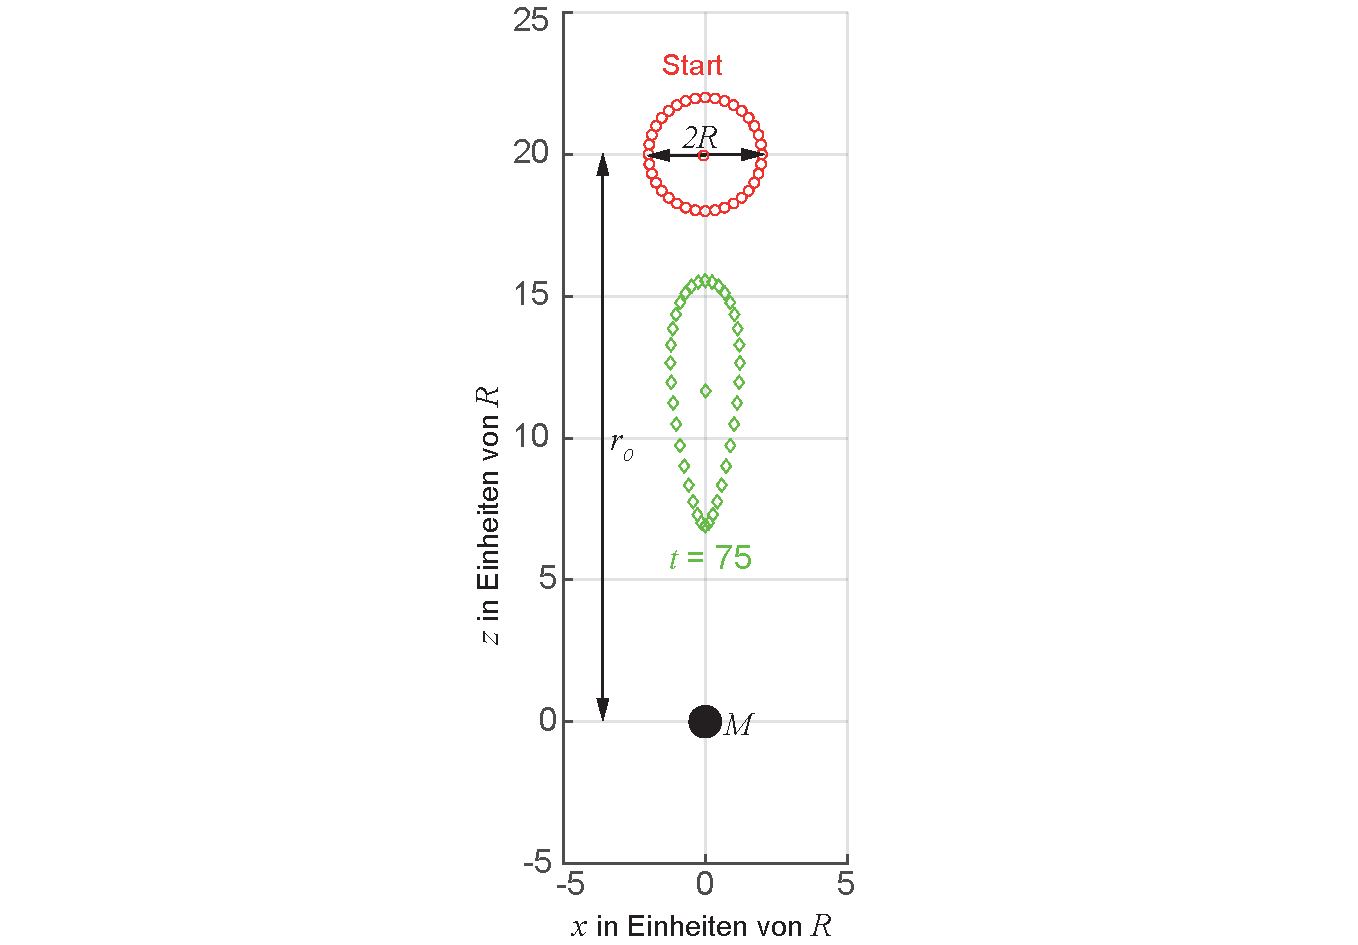
\includegraphics[width=\textwidth]{Gezeitenkraefte.pdf}
\caption[Gezeitenwirkung auf einen Ring.]{Gezeitenwirkung auf einen Ring aus 36 Massepunkten. Parameter: $r_0 = 20 R, R = 2, M\,G = 1.$}
\label{abb:hm_gezeiten01}
\end{figure}

Das Auseinanderbrechen von Himmelsk�rpern kann man durch die \emph{Roche-Grenze}
\footnote{�douard Albert Roche (1820 -- 1883) war ein franz�sischer Astronom und Mathematiker, der vor allem mit seinen theoretischen Arbeiten wichtige Beitr�ge zur Himmelsmechanik lieferte. 1850 berechnete er die nach ihm benannte kritische Distanz $r_\text{R}$, bei der ein Satellit unter der Wirkung von Gezeitenkr�ften zerrissen wird.}\index{Roche-Grenze}\index{Roche-Limit|textbf}\indexp{Roche, �douard Albert} (englisch \textit{Roche-Limit}) beschreiben.
Die Roche-Grenze ist die Entfernung eines Himmelsk�rpers der Dichte $\varrho_\text{S}$ von seinem Zentralk�rper der Dichte $\varrho_\text{Z}$ und des Radius $R_\text{Z}$, unterhalb derer der Himmelsk�rper aufgrund der Gezeitenkr�fte zerrissen wird.
Dabei wird angenommen, dass der K�rper nur von den eigenen Gravitationskr�ften zusammengehalten wird.
%Die Roche-Grenze ist damit die kleinste Umlaufbahn, in der der Himmelsk�rper den Zentralk�rper noch stabil umlaufen kann, ohne zerrissen zu werden.
Die Roche-Grenze ist gegeben durch
    \begin{align}
        r_\text{R} = \alpha\,R_\text{Z}\,\lk \frac{\varrho_\text{Z}}{\varrho_\text{S}}\rk^{\frac{1}{3}}\,, \label{eq:hm_rochelimit01}
    \end{align}
worin $\alpha$ ein materialabh�ngiger dimensionsloser Parameter zwischen $0$ und $1$ ist \cite{Bartelmann2015}.
Wir leiten die Beziehung \eqref{eq:hm_rochelimit01} in \probref{hm_rochelimit} her und sch�tzen auch f�r verschiedene Himmelsk�rper ihre Gr��e ab.

\subsection{Gezeiten im Erde-Mond-(Sonne)-System} \label{kap:hm_gezeiten_EM}

Man findet immer wieder etwas verwirrende oder zumindest unklare Darstellungen zu den Gezeiten des Erde-Mond-Systems (siehe dazu auch die Kommentare in Ref. \cite{Sawicki1999}).
Diese resultieren zumeist aus der unsauberen Betrachtung der verwendeten Koordinatensysteme \bzw der Eigenrotation der Erde im Verh�ltnis zur wahren \bzw scheinbaren Bewegung der Himmelsk�rper Mond und Sonne.
Wir wollen daher im Folgenden auf diese Themen besonderen Wert legen. \\
Als erstes wollen wir noch einmal den Ursprung der Gezeitenkr�fte beleuchten.
Im Kapitel Gezeiten des Bandes I hatten wir diese auf einen ausgedehnten K�rper wirkenden Kr�fte aus dem Gravitationspotential eines als Massepunkt angenommenen (da weit entfernten) Himmelsk�rpers hergeleitet.
Wir hatten in dieser Betrachtung im Inertialsystem offen gelassen, wie sich das System bei relativer Bewegung der die Gezeiten erzeugenden Himmelsk�rper zeitlich verh�lt. Das wollen jetzt nachholen.

\subparagraph{\textbf{\anf{Freier Fall} der Erde im Kraftfeld von Mond \bzw Sonne}}

Wir nutzen zun�chst zur physikalischen Beschreibung ein geozentrisches Koordinatensystem (\figref{hm_gezeiten02}), das aber \emph{nicht} mit der Erde mitrotiert und dessen Ursprung sich auf einem Kreis (\probref{hm_gezeiten01}) um den Schwerpunkt des Himmelsk�rper-Erde-Systems (der Himmelsk�rper ist entweder die Sonne oder der Mond) bewegt.
Da das gew�hlte KOS kein Inertialsystem ist, m�ssen alle Punkte der Erde in diesem System eine Scheinkraft $\vec{F}_\text{T}$ (Tr�gheitskraft, siehe Kapitel 1.2.2 im Band I) erfahren, die f�r alle Punkte des (starren) K�rpers gleich gro� ist.
Diese Kraft ist aber nichts anderes als die Schwerkraft, mit der die Erde im gew�hlten KOS "`frei f�llt"'.
Im Schwerpunkt des Erde-Himmelsk�rper-System (das ist der Ursprung des KOS) w�rde diese Tr�gheitskraft genau der Gravitationskraft entsprechen, ein mitbewegter Beobachter w�rde sich an dieser Stelle schwerelos f�hlen.
F�r alle Punkte der Erde wirkt daher als Gesamtkraft im gew�hlten KOS (\figref{hm_gezeiten02})
\begin{align}
    \vec{F}_\text{ges} = \vec{F}_\text{T} + \vec{F}_\text{G} = \vec{F}_\text{Gez} \,. \label{eq:hm_gezeiten11}
\end{align}
Aus Sicht eines Beobachters im nichtrotierenden geozentrischen KOS ist diese Gesamtkraft aus Gravitations- und Tr�gheitskraft also genau die Gezeitenkraft.
Wir k�nnen diese wie folgt aus \figref{hm_gezeiten02} herleiten:
\begin{align}
\begin{split}
    \vec{F}_\text{Gez} &= \frac{G\,M\,m}{r^3}\,\vec{r} - \frac{G\,M\,m}{r'{}^3}\,\vec{r}_\text{HK}~~
    \text{mit} ~~\vec{r}' = \vec{r} + \vec{R} = \vec{r} + R_\text{E}\frac{\vec{R}}{\left|\vec{R}\right|} \; , \\
		 \vec{r}'{}^2 &= \lk \vec{R} + \vec{r}\rk^2 = R^2 + r^2 + 2\,\lk \vec{R}\cdot\vec{r}\rk= \vec{r}'{}^2 = r^2\,\lk 1+\underbrace{\frac{R^2}{r^2}}_{\substack{\approx 0}} + \frac{2\,\vec{R}\cdot\vec{r}}{r^2}\rk \;.
\end{split} \label{eq:hm_gezeiten12}
\end{align}
In der N�herung $R/r \ll 1$ k�nnen wir $1/r'{}^3$ entwickeln:
\begin{align*}
    \frac{1}{ r'{}^3} = \lk  \vec{r}'{}^2\rk^{-\frac{3}{2}} \approx \lek r^2\lk 1+2\,\frac{\lk \vec{R}\cdot\vec{r}\rk}{r^2}\rk\rek^{-\frac{3}{2}} \approx \frac{1}{r^3}\,\lk 1-\frac{3}{\killA{2}}\,\killA{2}\frac{\lk \vec{R}\cdot\vec{r}\rk}{r^2}\rk \,.
\end{align*}
Damit ergibt sich: 
\begin{align}
     \vec{F}_\text{Gez} &\approx -\frac{G\,m\,M}{r^3}\,\lek \lk \vec{r} + \vec{R}\rk\,\lk 1-3\,\frac{\lk\vec{R}\cdot\vec{r}\rk}{r^2} \rk - \vec{r}\rek \approx -\frac{G\,m\,M}{r^3}\,\lk \vec{R} - \frac{3\,\lk \vec{R}\cdot\vec{r}\rk}{r^2} \lk \vec{r} + \vec{R}\rk \rk \,. \label{eq:hm_gezeiten13}
\end{align}
Wir sehen an \eqref{eq:hm_gezeiten13} zwei Dinge.
Zum einem heben sich die Hauptbetr�ge der Gravitationskraft und der Tr�gheitskraft, die proportional zu $\vec{r}/r^3$ sind, auf. Das ist ja genau f�r den freien Fall im Schwerpunkt zu erwarten.
Zum anderen wird nochmals deutlich, dass nur durch das inhomogene Gravitationsfeld ($\vec{F}(\vec{r}') \neq \vec{F}(\vec{r})$) �berhaupt eine Gezeitenkraft auftreten kann. 

\begin{figure}%
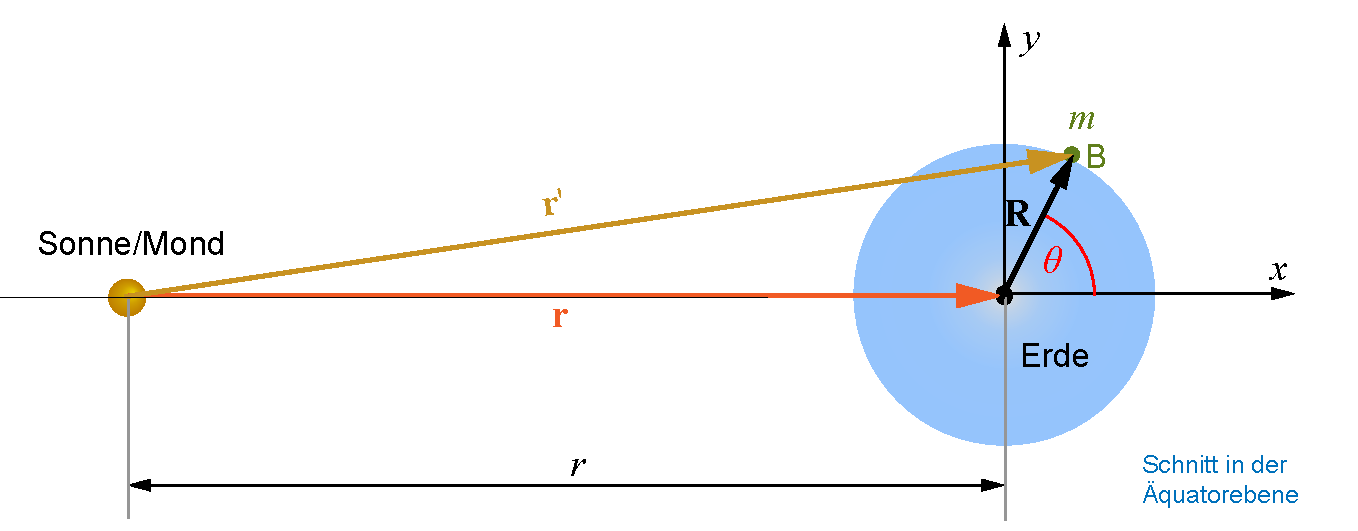
\includegraphics[width=\textwidth]{Gezeiten02.pdf}%
\caption[Zur Berechnung der Gezeitenkr�fte auf der Erdoberfl�che.]{Zur Berechnung der Gezeitenkr�fte auf der Erdoberfl�che (nicht ma�st�bliche Zeichnung). Beim Erde-Mond-System w�rde der gemeinsame Schwerpunkt leicht verschoben in Richtung Mond, aber noch innerhalb der Erde liegen. Die Bahnebenen von Erde und Mond werden vereinfacht als identisch mit der �quatorebene angenommen. B ist der Punkt eines Beobachters an einem beliebigen Punkt des �quators.}
\label{abb:hm_gezeiten02}%
\end{figure}

\subsection{Gezeitentheorie nach Newton}\indexp{Newton, Sir Isaac}\index{Gezeitentheorie nach Newton}\label{kap:hm_gezeiten:Newton}

\subparagraph{\textbf{Gleichgewichtsannahme in der Betrachtung einer nichtrotierenden Erde}}

\begin{figure}%
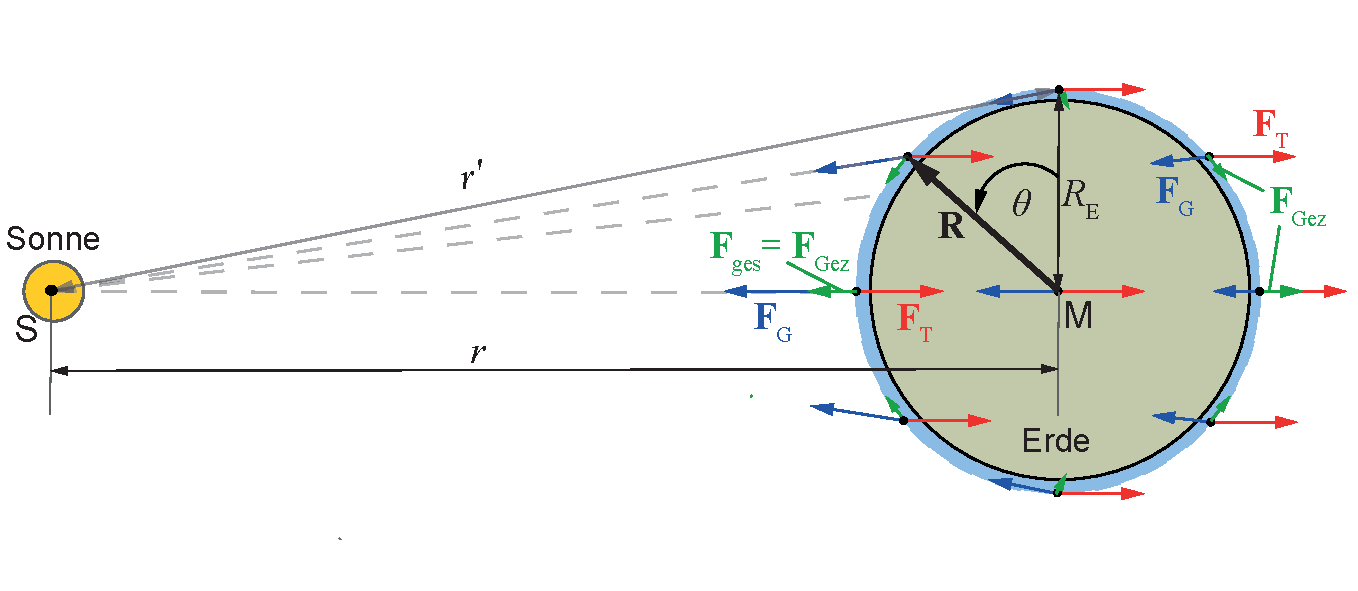
\includegraphics[width=\textwidth]{Gezeiten03S.pdf}%
\caption[Vektorielle Darstellung der Gezeitenkr�fte auf der Erdoberfl�che.]{Vektorielle Darstellung der Gezeitenkr�fte auf der Erdoberfl�che. In jedem Punkt der Erdoberfl�che wird die Vektorsumme aus Gravitations- und Tr�gheitskraft gebildet. Letztere ist �berall gleich gro� (nicht ma�st�bliche Zeichnung). Im Mittelpunkt der Erde heben sich die Kr�fte auf. Beim Erde-Mond-System w�rde der gemeinsame Schwerpunkt leicht verschoben in Richtung Mond, aber noch innerhalb der Erde liegen, an diesem w�rde ebenfalls die Gezeitenkraft verschwinden.}
\label{abb:hm_gezeiten03}%
\end{figure}

Wir betrachten nun, aus Sicht eines Beobachters auf der Erde, die vertikalen und horizontalen Komponenten\footnote{Aus Sicht eines Beobachters im Inertialsystem sind das die radialen \bzw tangentialen Komponenten.} der Gezeitenkraft \bzw der Gezeitenbeschleunigung\footnote{An Gleichung \eqref{eq:hm_gezeiten13} kann man erkennen, dass $F_\text{Gez} \approx \lk \vec{R}\cdot\vec{r}\rk r^{-5}$ ist, was auf ein Quadrupolpotential\index{Quadrupol} f�r die Gezeitenkraft hinweist.\index{Multipolentwicklung} Wir werden uns mit der Multipolentwicklung von Feldern und anderen physikalischen Gr��en in \kap{hm_potentialtheorie}, sowie in der Astrodynamik (Kap. \ref{chap:adyn}) und in der Elektrodynamik (Band IV) besch�ftigen. Hier gen�gt zu wissen, dass eine Quadrupolgr��e dadurch gekennzeichnet ist, dass ihr Potential eine $r^{-5}$-Abh�ngigkeit hat und in zwei zueinander orthogonalen Richtungen auf Grund des Skalarproduktes $\lk \vec{R}\cdot\vec{r}\rk$ unterschiedliche funktionale Abh�ngigkeit von einem Parameter wie \zb dem Winkel zwischen $\vec{R}$ und $\vec{r}$ zeigt.} (\figref{hm_gezeiten03}). Diese k�nnen mit dem Winkel $\theta$ und $\left|\vec{R}\right| = R_\text{E}$ und $g_0= G\,M/r^2$ wie folgt geschrieben werden:
\begin{align}
    g_\text{Gez,H} &= \frac{F_\text{Gez,H}}{m} = -3\,\frac{G\,\killA{m}\,M}{\killA{m}\,r^3}\,R_\text{E}\,\cos\theta\,\sin\theta 
		                =-\frac{3}{2}\,g_0\,\frac{R_\text{E}}{r}\,\sin 2\theta \,. \label{eq:hm_gezeiten14}
\end{align}
Analog folgt f�r die vertikale Komponente aus \eqref{eq:hm_gezeiten13}
\begin{align}
    g_\text{Gez,V} &= +g_0\,\frac{R_\text{E}}{r}\lk 3\cos^2\theta-1\rk = \frac{3}{2}\,g_0\,\frac{R_\text{E}}{r}\lk \cos2\theta+\frac{1}{3}\rk \,. \label{eq:hm_gezeiten15}
\end{align}
Der letzte Term gibt einen konstanten, vom Winkel $\theta$ unabh�ngigen Beitrag $\lk \frac{1}{2}\,g_0\,\frac{R_\text{E}}{r}\rk$ zur Erdbeschleunigung $g_0$ und ist f�r die weitere Betrachtung irrelevant.
Wir k�nnen also n�herungsweise schreiben:
\begin{align}
    g_\text{gez,V} \approx \frac{3}{2}\,g_0\,\frac{R_\text{E}}{r}\,\cos 2\theta \,. \label{eq:hm_gezeiten15a}
\end{align}

Die Erdbeschleunigung $g_\text{E}$ ist durch $g_\text{E} = G\,m_\text{E}/R_\text{E}{}^2$ gegeben, daher k�nnen wir f�r das maximale Verh�ltnis der Gezeitenbeschleunigung zur Erdbeschleunigung schreiben:
\begin{align}
\begin{split}
    \text{Mond:} ~~~~ \left|\frac{g_\text{Gez,M}}{g_\text{E}}\right| 
		 &= \frac{3}{2}\,\frac{m_\text{M}}{m_\text{E}}\,\frac{R_\text{E}{}^3}{r_\text{EM}{}^3} = \frac{3}{2}\,\xi_\text{M}\, R_\text{E} \approx \SI{8.4e-8}{} \,,\\
    \text{Sonne:} ~~~~\left|\frac{g_\text{Gez,S}}{g_\text{E}}\right| 
		 &= \frac{3}{2}\,\frac{m_\text{S}}{m_\text{E}}\,\frac{R_\text{E}{}^3}{r_\text{ES}{}^3} = \frac{3}{2}\,\xi_\text{S}\, R_\text{E}\approx  \SI{3.9e-8}{} \,.
\end{split} \label{eq:hm_gezeiten16}
\end{align}
Hierin ist 
\begin{align}
	  \xi_\text{M} = \frac{m_\text{M}}{m_\text{E}}\,\frac{R_\text{E}{}^3}{r_\text{EM}{}^3} = \frac{m_\text{M}}{m_\text{E}}\,\frac{R_\text{E}{}^3}{a_\text{EM}{}^3} \approx \SI{5.62e-8}{} \label{eq:hm_xi_gezeiten}
\end{align}
ein Ma� f�r die Gezeitenst�rke des Mondes und analog $\xi_\text{S}$ f�r die Sonne, wobei wir f�r $r_\text{EM}$ den Abstand der Mittelpunkte von Erde und Mond $a_\text{EM}$ gesetzt haben.  Die Gezeitenkr�fte betragen also nur weniger als das $10^{-7}$-fache der Erdbeschleunigung, k�nnen aber dennoch durch ihre Horizontalkomponenten eine gro�e Wirkung auf die Ozeane aus�ben.%
\footnote{Man liest immer wieder, dass die Tiden durch \anf{Anheben} des Wassers, \dh die Vertikalkomponente entstehen. Das ist nach \eqref{eq:hm_gezeiten16} wohl kaum m�glich!}
Das erkannte auch schon Newton.
Er nahm f�r die nicht rotierende Erde an, dass die Gezeitenkr�fte wegen der relativ langsamen Bewegung der die Gezeiten erzeugenden Himmelsk�rper eine station�re Form der Wasseroberfl�che der Ozeane ausbilden k�nnen. F�r eine im Gleichgewichtsfall ausgeformte Wasserh�lle muss die Oberfl�che so sein, dass durch die Oberfl�chenverformung die Horizontalkomponente der Gezeitenkraft kompensiert wird. Eine entsprechende Rechnung (siehe \kap{hm_potentialtheorie}) zeigt, dass die so geformte Wasserh�lle ein Ellipsoid der Form 
\begin{align} 
    R_\text{W}\lk \theta \rk = R_\text{E}\,\lk 1 - \frac{2}{3}\,\varepsilon\, \mathcal{P}_2 \lk \cos \theta \rk \rk = R_\text{E}\,\lk 1 - \frac{2}{3}\,\varepsilon \ \lk \frac{3}{2} \cos^2 \theta - \frac{1}{2} \rk \rk \, \label{eq:hm_gezeiten17a}
\end{align}
ergibt, worin $R_\text{E}$ der mittlere Erdradius ist, der n�herungsweise gleich dem Radius der ungest�rten Wasserh�lle der weltumspannenden Ozeane $R_\text{W,0}$ gesetzt wird $(R_\text{E} \approx R_\text{W,0})$.  $\mathcal{P}_2 \lk \cos \theta \rk$ ist das Legendre-Polynom 2.\,Ordnung (siehe \kap{hm_potentialtheorie} und die \onlineZ) und $\varepsilon$ die Elliptizit�t (Abplattung) des Ellipsoids. Diese ist definiert �ber
\begin{align}
	\varepsilon = \frac{R_\text{A} - R_\text{P}}{R_\text{E}} \,, \label{eq:hm_gezreibung03}
\end{align}
worin $R_\text{A},\, R_\text{P}$ die  Radien der Erde am �quator \bzw am Pol (Richtung Symmetrieachse) bedeuten, wie man leicht �berpr�fen kann. 
H�ufig wird die Abh�ngigkeit des Radius von $\theta$ auch n�herungsweise in der Form 
\begin{align} 
    R_\text{W}\lk \theta\rk \approx R_\text{E}\,\lk 1 + \frac{h}{R_\text{E}}\,\cos 2\theta \rk  \label{eq:hm_gezeiten17}
\end{align}
geschrieben, worin $h$ die Anhebung der Wasserh�lle durch die Gezeitenkr�fte ist. 
Wir bestimmen aus \eqref{eq:hm_gezeiten17} den Neigungswinkel $\gamma$ der Wasseroberfl�che als Funktion des Winkels $\theta$ relativ zur Lotlinie.\footnote{Hier nehmen wir implizit an, dass die Dichte des Ozeanwassers verschwindend gering ist und es bleibt zun�chst auch unber�cksichtigt, dass sich der feste Erdk�rper ebenfalls durch die Gezeiten verformt.} Wir erhalten:
\begin{align}
  \gamma &\approx \tan \gamma = \frac{g_\text{Gez,H}}{g_\text{E}} = -\frac{2h}{R_\text{E}}\,\sin 2\theta ~~\rightarrow ~~ \varepsilon = -\frac{2\,h}{R_\text{E}} = -\frac{g_\text{Gez,H}}{g_\text{E}}\,. \label{eq:hm_gezeiten_epsilon}
\end{align}
Offensichtlich ist $\varepsilon < 0$ was mit der Definition eines prolaten Ellipsoiden �bereinstimmt. Die Wasserh�hen durch die Gezeitenkr�fte von Mond und Sonne sind dann:
\begin{align}
\begin{split}
    \Delta h_\text{M} &= 2h_\text{M} = \frac{3}{2}\,\xi_\text{M}\,R_{E} \approx \SI{0.54}{\metre} ~~\text{bzw.} ~~\Delta h_\text{S} = 2h_\text{S} = \frac{3}{2}\,\xi_\text{S}\,R_{E}{} \approx \SI{0.24}{\metre} \,.
\end{split} \label{eq:hm_gezeiten18}
\end{align}

\begin{figure}%
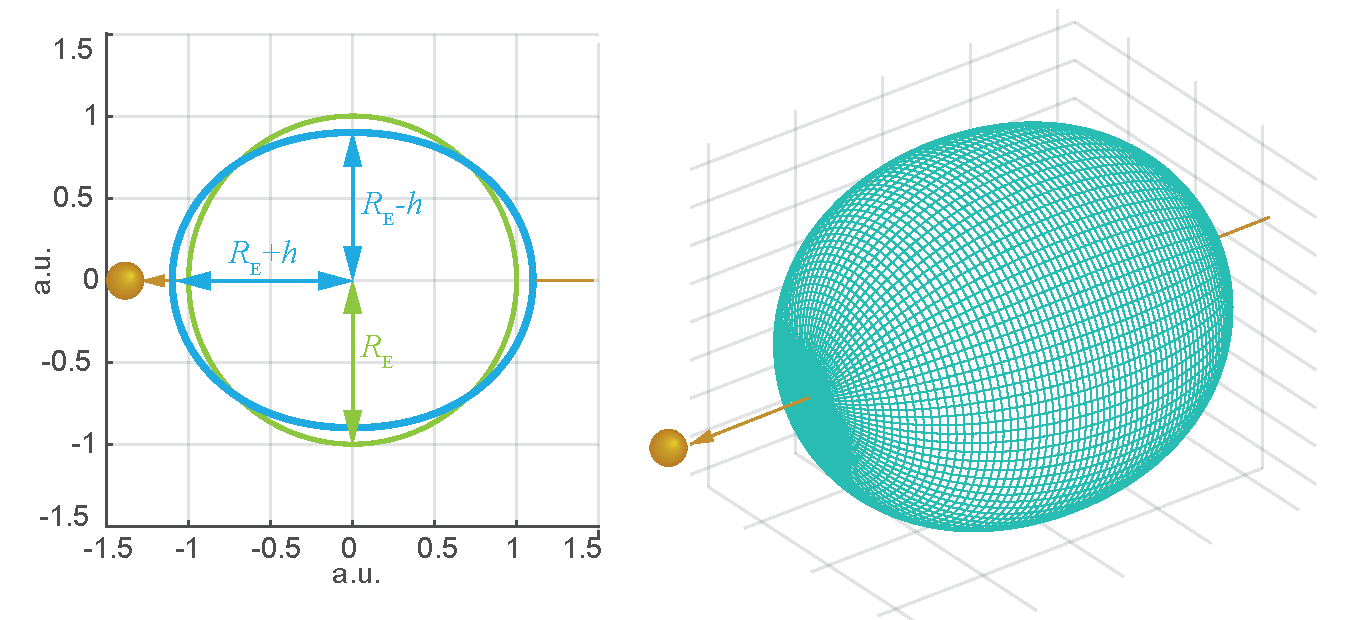
\includegraphics[width=\textwidth]{Gezeiten05.pdf}%
\caption[Gezeitenellipsoid.]{Gezeitenellipsoid. Stark �berh�hte Darstellung, mit $h \approx 0.1 R_\text{E}$. F�r die realen Gezeiten der Ozean auf der Erde ist $h < \SI{1e-7}{}R_\text{E}$.}
\label{abb:hm_gezeiten05}%
\end{figure}

\figref{hm_gezeiten05} zeigt das sich ausbildende Ellipsoid nach Gleichung \eqref{eq:hm_gezeiten17}.
Eine genaue Rechnung zeigt, dass bei einer Annahme der Form der Wasserh�lle nach \eqref{eq:hm_gezeiten17} das Volumen der Wasserh�lle nicht exakt konstant ist, was der Annahme einer inkompressiblen Fl�ssigkeit widerspricht. Da $\Delta h \ll R_\text{E}$ ist die N�herung f�r unsere Rechnungen aber sehr gut zu verwenden. Wir verweisen auch auf die \textbf{�bungen} \ref{prob:hm_gezeiten01} und \ref{prob:hm_gezeiten04}.

\subparagraph{\textbf{Ber�cksichtigung der Eigenrotation der Erde}}

Bisher haben wir nur die Bewegung von Erde und Mond um den gemeinsamen Schwerpunkt in unseren Betrachtungen ber�cksichtigt.%
\footnote{Im Folgenden beziehen wir uns, wenn nicht anders erw�hnt, nur noch auf den Mond. Alle �berlegungen gelten aber prinzipiell genauso f�r die Sonne.}
Danach w�re der Hochwasser-Berg nach Newtons Annahme der instantanen Ausbildung des Gezeitenellipsoids immer auf der Linie Schwerpunkt-Mondmittelpunkt fixiert (\probref{hm_gezeiten01}).
Es w�rde sich daher nur zweimal alle 27.32 Tage Hochwasser und Niedrigwasser ergeben, n�mlich jeweils beim oberen und unteren Meridiandurchgang des Mondes%
\footnote{Man �berlege sich, warum wir die synodische Umlaufzeit des Mondes $(T_\text{synod} = 27.32\,\mathrm{d})$ verwenden m�ssen!}.
Ber�cksichtigen wir jetzt die Erdrotation, wandert die Erdoberfl�che sozusagen st�ndig unter den Hochwasser-Bergen und Niedrigwasser-T�lern in �stlicher Richtung davon, oder bewegt sich anders gesprochen der Hochwasser-Berg in westlicher Richtung um die Erde.\\
F�r die mathematische Beschreibung wechseln wir nun in ein echtes mitrotierendes geozentrisches Koordinatensystem.
Der Winkel $\theta$ wird dann zeitabh�ngig und \ia eine Funktion $\theta(\alpha\lk t\rk, \delta\lk t\rk)$, worin $\alpha$ und $\delta$ die Rektaszension \bzw die Deklination des Mondes sind.
Wir wollen zun�chst der Einfachheit halber eine Deklination des Mondes von $\delta = 0 $ annehmen, \dh der Mond steht �ber dem �quator im Zenit.
Auch an \eqref{eq:hm_gezeiten14} erkennt man, dass es wegen der $\sin 2\theta$--Abh�ngigkeit zwei Hochwasser-Tiden pro Tag geben muss.
Beim Mond muss man die Eigenbewegung ber�cksichtigen, die immerhin $360\degree / 27.32\,\mathrm{d} = 13.177\degree/ \mathrm{d}$ betr�gt.
Im Mittel (Kreisbahn des Mondes angenommen) ist deshalb der Mondtag um $\SI{50}{\min}\,\SI{24}{\second}$ l�nger als der Sonnentag, weswegen der mittlere zeitliche Abstand zwischen zwei Hochwasser ca. $\SI{12}{\hour}\,\SI{25}{\min}$ betr�gt.
Man kann auch sagen, dass ein Pegelstab eines Beobachters quasi in $\SI{24}{\hour}\,\SI{50}{\min}$ einmal durch die ann�hernd station�re Wasserh�lle \anf{pfl�gt} (\probref{hm_gezeiten03}).
In \figref{hm_gezeiten04} haben wir die Wirkung der Horizontalkomponenten auf die Ozeanh�lle der Erde noch einmal schematisch dargestellt.\\

\begin{figure}%
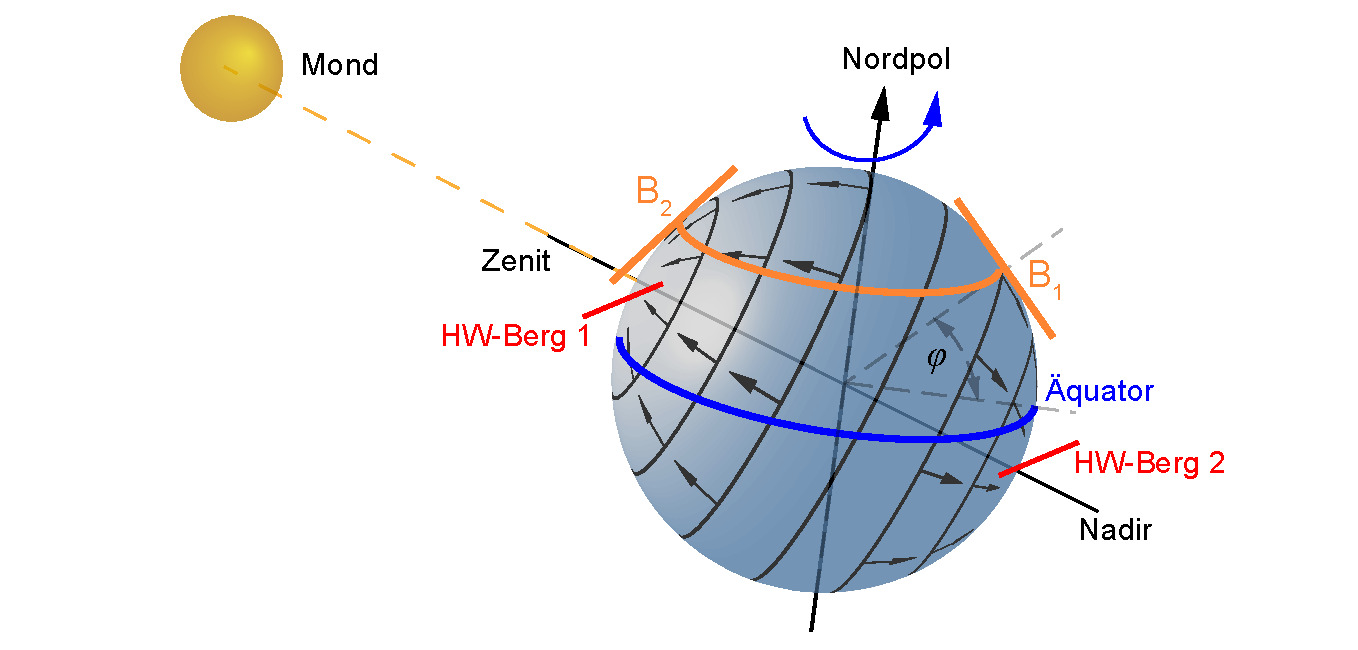
\includegraphics[width=\textwidth]{Gezeiten04.pdf}%
\caption[Gezeiten des Mondes auf der Erde.]{Gezeitenwirkung des Mondes auf der Erde. Ohne Erddrehung w�rde sich nur zweimal alle 27.32 Tage Hochwasser und Niedrigwasser ergeben, n�mlich jeweils beim oberen und unteren Meridiandurchgang des Mondes. Mit Erddrehung ergibt sich nach der Newtonschen Gleichgewichtstheorie pro Tag f�r einen Beobachter auf einen Breitenkreis $\varphi$ zwei Hochwasser und zwei Niedrigwasser, letztere werden durch einen Niedrigwasser-Ring um die Polachse herum gebildet. Man erkennt auch, dass die aufeinanderfolgenden Hochwasserst�nde f�r die Beobachter $\mathrm{B}_1$ und $\mathrm{B}_2$ \ia unterschiedlich gro� sind.}
\label{abb:hm_gezeiten04}%
\end{figure}

Die Newtonsche Gezeitentheorie liefert trotz ihrer Einfachheit schon viele grundlegende richtige Ergebnisse.
Insbesondere lassen sich die Ph�nomene von Spring- und Nipptiden durch unterschiedliche Stellungen von Erde, Mond und Sonne zueinander erkl�ren, ebenso wie die sogenannten astronomisch bedingten "`Ungleichheiten"', die durch Exzentrizit�ten und Neigungen der Bahnen von Erde und Mond erkl�rt werden k�nnen. (\probref{hm_gezeiten03}).
Die absolut berechneten H�hen $\SI{54}{\centi\metre}$ f�r Mondtide \bzw $\SI{24}{\centi\metre}$ f�r maximale Sonnentide gelten aber bestenfalls im freien Ozean, fern von K�sten und selbst da nur eingeschr�nkt.

Nicht erkl�rbar ist durch die Newtonsche Theorie auch, dass die tats�chlich beobachteten Hochwasser-Zeiten nicht, wie nach der Theorie zu erwarten, mit den Kulminationszeiten des Mondes �bereinstimmen. Wir m�ssen also die Theorie verbessern, was wir in \kap{hm_gezeiten_Laplace} beschreiben wollen. 
Zun�chst werden wir aber mit der Potentialtheorie eine breit anwendbare Methode kennenlernen, mit der wir auch noch einmal die Ergebnisse der Newtonschen Gezeitentheorie elegant herleiten wollen und die wir anschlie�end im \kap{hm_gezeitenreibung} sehr vorteilhaft anwenden k�nnen.

\newpage
\subsection{Grundlagen der Potentialtheorie der Gravitation} \label{kap:hm_potentialtheorie}

\subsubsection{Gravitationspotential einer beliebigen Masseverteilung} \label{kap:hm_pot_general_distrib}

Wir wollen zun�chst die grundlegende Beziehung f�r die Berechnung eines Gravitationspotentials einer beliebigen Massenverteilung herleiten. Im Kapitel Physik der Bewegung (Band I) hatten wir dargestellt, wie die Gravitationskraft zwischen zwei Massepunkten aus dem Gravitationspotential berechnet werden kann.
Wir betrachten dazu eine beliebige Anzahl von Massepunkten $m_i \lk i=1\ldots N\rk$. Wir stellen uns vor, dass man nach und nach alle Massen aus dem Unendlichen in eine Anordnung bringt, nach der die Massen $m_i$ jeweils an den Orten $\vec{r}_i$ liegen. Dabei wird durch die Gravitationskraft Arbeit verrichtet werden, die da erstere konservativ ist als Differenz eines Potentials geschrieben werden kann:
    \begin{align*}
        W_i = m_i\,\bigintsss\limits_\infty^{\vec{r}_i}\vec{\nabla}U \cdot \D\vec{s}_i = m_i\lek U\lk \vec{r}_i\rk - \underbrace{U\lk\infty\rk}_{=0}\rek\,.
    \end{align*}
Als gravitative Selbstenergie $U_\text{S}$ aller Massen $m_i$ kann die Summe der Arbeiten $W_i$ verstanden werden. Bei der Doppelsummenbildung muss man einen Faktor $\frac{1}{2}$ anwenden, damit bei der Summe �ber $i$ und $j$ die einzelnen Arbeiten nicht doppelt gez�hlt werden.\footnote{Beispiel f�r 3 Massen: Wir bringen zun�chst die Masse $m_1$ an die Position $\vec{r}_1$, dann $m_2$ an die Position $\vec{r}_2$, schlie�lich $m_3$ an die Position $\vec{r}_3$. Da aber die Reihenfolge egal ist, addieren wir die Arbeiten $W_\text{A} = W_1(\vec{r}_1)+W_2(\vec{r}_1,\vec{r}_2)+W_3(\vec{r}_1,\vec{r}_2,\vec{r}_3) \text{und} W_\text{B} = W_1(\vec{r}_1)+W_3(\vec{r}_1,\vec{r}_3)+W_2(\vec{r}_1,\vec{r}_3,\vec{r}_2)$ und halbieren $W_\text{A}+W_\text{B}$.}
    \begin{align*}
        E_\text{S} &= -\frac{1}{2}\,G\,\sum_{\substack{i,j=1\\i\neq j}}^N\,\frac{m_i\,m_j}{|\vec{r}_i-\vec{r}_j|} = \frac{1}{2}\sum_{i=1}^N W_i = \frac{1}{2}\sum_{i=1}^N m_i\,U_i \\ 
     & \text{mit}~~~ U_i\lk \vec{r}_j\rk = -G\sum_{\substack{j=1 \\ i\neq j}}^N \frac{m_j}{|\vec{r}_i-\vec{r}_j|}\,. 
    \end{align*}
    Von der Summe f�r $U_i\lk \vec{r}_j\rk$ kommt man leicht zum Integral f�r eine kontinuierliche Massenverteilung\footnote{Im strengen Sinne erfolgt die Berechnung �ber die Methode der \textit{Greenschen Funktionen}, die wir in der Potentialtheorie f�r elektrische Felder in der Elektrodynamik (Band IV) kennen lernen werden. Siehe auch \cite{Otto2019, Fischer2018} und \cite{Riley2006, Felder2016}}:
    \begin{align}
      U\lk \vec{r}\rk = -G\bigintsss\frac{\varrho\lk\vec{r}'\rk}{|\vec{r}'-\vec{r}|}\,d^3\,\vec{r}' \; . \label{eq:hm_pot_theo01}
    \end{align}
    Dies ist der allgemeine Ausdruck f�r ein Gravitationspotential
    $U\lk \vec{r}\rk$, das durch eine kontinuierliche Massenverteilung
    $\varrho\lk \vec{r}\rk$ hervorgerufen wird
    (\figref{hm_pot_general_distrib}).

    \begin{figure}[H]
	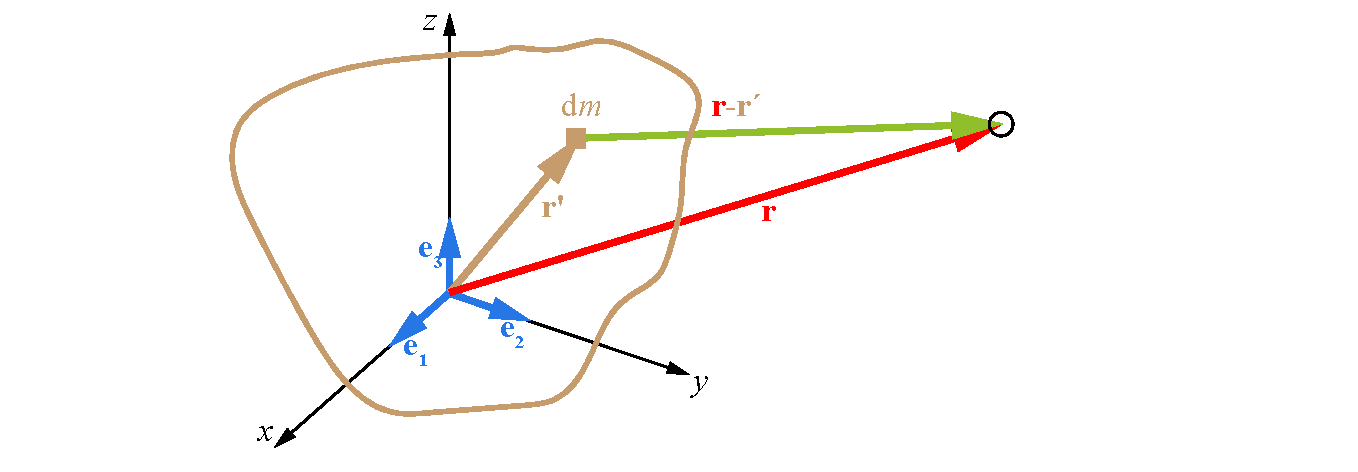
\includegraphics[width=\textwidth]{KOSGravPotential_allg.pdf} 
	\caption[Gravitationspotential f�r kontinuierliche Massenverteilungen.]{Zur Herleitung des Gravitationspotentials f�r kontinuierliche Massenverteilungen.}
	\label{abb:hm_pot_general_distrib}
\end{figure}

\subsubsection{Gravitationspotential einer rotationssymmetrischen Masseverteilung} \label{kap:hm_pot_rotsymm_distrib}

Oft haben wir Massenverteilungen vorliegen, die achsen- \bzw rotationssymmetrisch sind (\figref{hm_pot_rotsymm_distrib}). Die Idee ist nun, mit einer Behandlung des physikalischen Problems in sph�rischen Koordinaten eine angepasste und damit einfachere und elegantere Darstellung zu finden.\\
Wir schreiben \eqref{eq:hm_pot_theo01} in sph�rischen Koordinaten, die wir hier mit $r,\,\phi,\,\theta$ bezeichnen wollen. �ber die Symmetrie-Koordinate $\phi$  kann integriert werden:
    \begin{align}
      U\lk r,\theta\rk = -2\pi\,G\,\bigintsss\limits_0^\infty\bigintsss\limits_0^\pi
      \langle \frac{r'^2\,\sin\theta'\,\varrho\lk r',\theta'\rk}
      {|\vec{r}-\vec{r}'|}\rangle  \,\D r'\, \D\theta' \,,
      \label{eq:hm_pot_theo02} 
    \end{align}

\begin{figure}[H]
	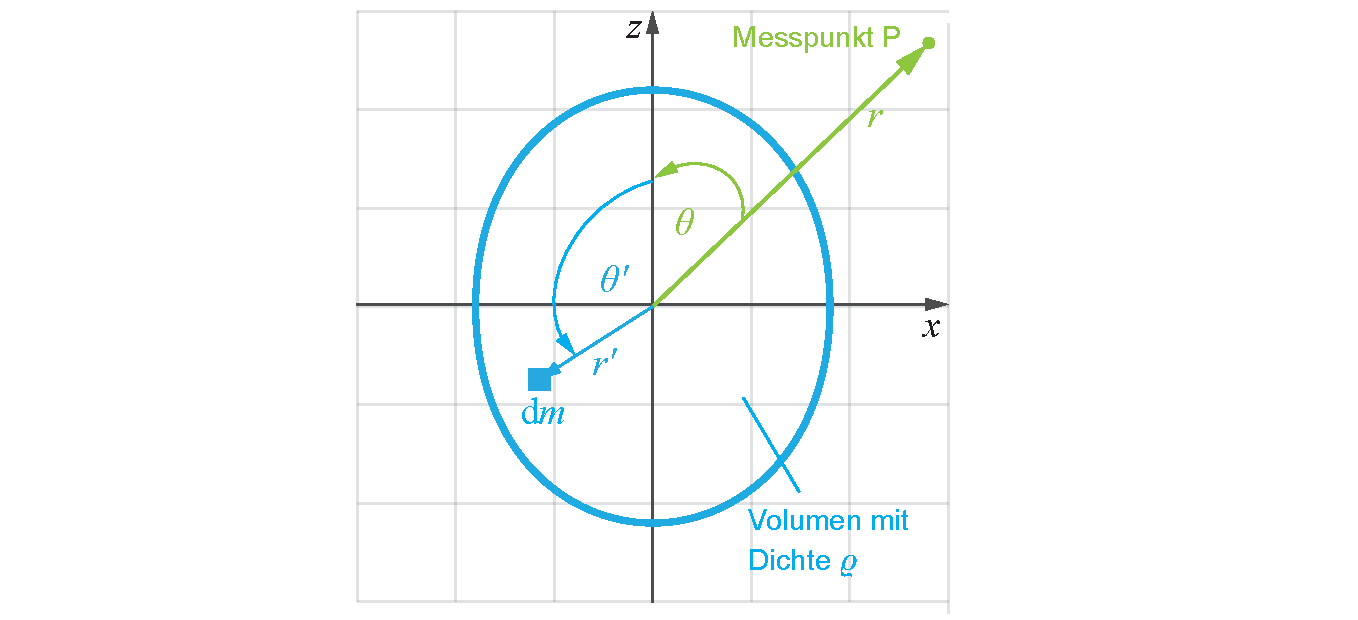
\includegraphics[width=\textwidth]{KOSGravPotential_axial.pdf} 
	\caption[Gravitationspotential f�r rotationssymmetrische Massenverteilungen.]{Zur Herleitung des Gravitationspotentials f�r rotationssymmetrische Massenverteilungen.}
	\label{abb:hm_pot_rotsymm_distrib}
\end{figure}

wobei
    \begin{align}
      \langle \frac{1}{|\vec{r}-\vec{r}'|} \rangle
      = \frac{1}{2\pi}\int\limits_0^{2\pi}\frac{\D\phi'}{|\vec{r}-\vec{r}'|}
      \,\D\phi'\label{eq:hm_pot_theo03} \,,
    \end{align}
eine Mittelung (Integral) �ber die Symmetrie-Koordinate $\phi'$ ist. Wir haben ja bereits mehrfach den Term 
    \begin{align*}
        \frac{1}{|\vec{r}-\vec{r}'|} = \lk r^2-2\vec{r}\,\vec{r}' + r'^2\rk^{-\frac{1}{2}} \,,
    \end{align*}
f�r $|\vec{r}|>|\vec{r}'|$ entwickelt (\zb \eqref{eq:hm_gezeiten12}) und schreiben jetzt das darin auftretende Skalarprodukt $\vec{r}\,\vec{r}'$ als:
    \begin{align}
    \begin{split}
        \vec{r}\,\vec{r}' &= r\,r'\,Q\lk \theta,\theta',\phi'\rk \,, \\
        Q\lk \theta,\theta',\phi'\rk &= \sin\theta\,\sin\theta'\,\cos\phi' + \cos\theta\,\cos\theta' \; ,
    \end{split} \label{eq:hm_pot_theo04}
    \end{align}
woraus folgt:
    \begin{align}
         \frac{1}{|\vec{r}-\vec{r}'|} = &\frac{1}{r} \lek 1 + \frac{r'}{r}\,Q + \frac{1}{2}\,\lk \frac{r'}{r} \rk^2 \lk 3Q^2 - 1 \rk + \mathcal{O} \lk \frac{r'}{r}\rk^3 \rek \,. \label{eq:hm_pot_theo05}
    \end{align}
Wir k�nnen jetzt das Integral \eqref{eq:hm_pot_theo03} gliedweise in \eqref{eq:hm_pot_theo05} ausf�hren und erhalten bis zur zweiten Ordnung in $Q$:
\begin{align*}
  \langle 1 \rangle &= \frac{1}{2\pi}\int\limits_0^{2\pi}\D\phi' = 1\,,\qquad
	\langle Q \rangle = \cos\theta\,\cos\theta' \,,\\
  \langle Q^2 \rangle &= \frac{1}{2}\,\sin\theta\,\sin^2\theta' + \cos^2\theta\,\cos^2\theta' \\
	                    &= \frac{1}{3} +\frac{2}{3}\,\lk \frac{3}{2}\,\cos^2\theta-\frac{1}{2}\rk\lk \frac{3}{2}\,\cos^2\theta'-\frac{1}{2}\rk\,.
    \end{align*}
Damit erhalten wir:
    \begin{align}
        \frac{1}{|\vec{r}-\vec{r}'|} = \frac{1}{r} \bigg[ 1 &+ \frac{r'}{r} \cos\theta\,\cos\theta' \nonumber \\
				       &+ \lk \frac{r'}{r} \rk^2\,\frac{1}{2}\,\lk 3\cos^2\theta-1\rk\,\frac{1}{2}\,\lk 3\cos^2\theta'-1\rk + \mathcal{O} \lk \frac{r'}{r}\rk^3  \bigg] \,. \label{eq:hm_pot_theo06}
    \end{align}
Mit Hilfe der \emph{Legendre-Polynome}\footnote{Adrien-Marie Legendre (1752--1833) war ein franz�sischer Mathematiker, der besonders f�r seine Arbeiten zu den nach ihm benannten Legendre-Polynomen und den elliptischen Integralen bekannt ist.}\indexp{Legendre, Adrien-Marie }\index{Polynome!Legendre-} $\PL n$ (siehe \cite{Riley2006, Felder2016} und die als Anhang \onlineZ), kann man die Beziehung \eqref{eq:hm_pot_theo03} elegant schreiben als:
    \begin{align}
        U\lk r,\theta\rk &= \sum_{n=0}^\infty\Phi_n\lk r\rk\,\PL n\lk \cos\theta\rk\,, \label{eq:hm_pot_theo07}
	  \end{align}
    worin die $\PL n$ durch die \gls{legendrePol} 
    \begin{align}
		\begin{split}
        \PL n\lk \cos\theta\rk =
				\begin{cases}
            1 & n=0 \\
            \cos\theta & n=1 \\
            \frac{1}{2}\,\lk 3\cos^2\theta-1\rk & n=2 \\
            \frac{1}{2}\,\lk 5\cos^3\theta-\cos\theta\rk & n=3 \\
            \ldots & n \geq 4       
				\end{cases}
		\end{split} \label{eq:hm_pot_theo07a}
    \end{align}
gegeben sind und die $\Phi_n\lk r\rk$ durch
    \begin{align}
        \Phi_n\lk r\rk = &-\frac{2\pi\,G}{\lk n+\frac{1}{2}\rk\,r^{n+1}}\,\int\limits_0^r r'^{n+2}\,\varrho_n\lk r'\rk\, \D r' - \frac{2\pi\,G\,r^n}{n+\frac{1}{2}}\,\int\limits_r^\infty r'^{1-n}\,\varrho_n\lk r'\rk \,\D r' \,. \label{eq:hm_pot_theo08}
    \end{align} 
Dabei haben wir folgende Entwicklungen benutzt:
    \begin{align*}
      \text{f�r}~r>r':~~  \frac{1}{|\vec{r}-\vec{r}'|} &= \frac{1}{r} \sum\limits_{n=0}^\infty \lk \frac{r'}{r}\rk^n \PL n(\cos\theta)\, \PL n(\cos\theta')\,~~\text{\bzw} \\
      \text{f�r}~r<r':~~  \frac{1}{|\vec{r}-\vec{r}'|} &= \frac{1}{r'} \sum\limits_{n=0}^\infty \lk \frac{r}{r'}\rk^n \PL n(\cos\theta)\, \PL n(\cos\theta')\,.
		\end{align*}
Die Beziehung \eqref{eq:hm_pot_theo08} k�nnen wir auch schreiben als:
		\begin{align*}
        \Phi_n\lk r\rk = \,&T_{1n}\lk r\rk + T_{2n}\lk r\rk \,. 
    \end{align*}
Dabei haben wir mit 
    \begin{align}
        \varrho\lk r',\theta'\rk = \sum_{n=0}^\infty \varrho_n\lk r'\rk\,\PL n\lk \cos\theta'\rk \label{eq:hm_pot_theo09}
    \end{align}
eine Entwicklung der Dichtefunktion nach \gls{legendrePol} verwendet, was immer m�glich ist, da die $\PL n$ ein vollst�ndiges Orthonormalsystem bilden \cite{Riley2006, Felder2016}. Mit \eqref{eq:hm_pot_theo07} bis \eqref{eq:hm_pot_theo09} haben wir also folgendes erreicht:
    \begin{enumerate}
        \item [1.] Wir haben die Variablen $\theta$ und $r$ (\bzw $\theta'$ und $r'$) jeweils separiert. 
        \item [2.] Wir haben eine Reihenentwicklung mit Ordnungen von ${r'}/{r}$ \bzw ${r}/{r'}$ errhalten.
        \item [3.] Wir konnten den Radialanteil $\Phi_n(r)$ in zwei Anteile $T_{1n}$ und $T_{2n}$ separieren, wobei die Anteile $T_{2n}$ nur relevant sind, wenn man das Potential innerhalb der Massenverteilung berechnen will.
		\end{enumerate}
Wir werden im Folgenden an zwei Spezialf�llen verdeutlichen, wie man mit den Beziehungen \eqref{eq:hm_pot_theo07} und \eqref{eq:hm_pot_theo08} das Potential $U(\vec{r})$ berechnet. 

\subsubsection{Gravitationspotential f�r zwei Spezialf�lle} \label{kap:hm_pot_special cases}

\subparagraph{\textbf{Homogene Kugel mit Dichte $\hat{\varrho}_0$ und Radius $R$ }}

Es gilt, da keine Winkelabh�ngigkeit vorliegt:
\begin{align*}
  \varrho_0\lk r'\rk
  &= \begin{cases}
    \hat{\varrho}_0 & r'\leq R \\
    0 & r'> R
  \end{cases} ~~\text{und}~~\varrho_n\lk r'\rk = 0 ~~~~ \forall\, n \geq 1\,.
\end{align*}
Dann folgt f�r $r>R$:
\begin{align*}
  T_{10} &= -\frac{4\pi\,G}{r}\,\int\limits_0^R \hat{\varrho}_0\,{r'}^2\,\D'r = \frac{4\pi\,G}{r}\,\frac{1}{3}\,\hat{\varrho_0}\,R^3 = -\frac{M\,G}{r}\,,\quad
  T_{20} &= 0 \,, \\
  \rightarrow ~~~~ U\lk r\rk &= -\frac{M\,G}{r} \,,
\end{align*}
was wir nat�rlich schon wussten. Das Gravitationspotential einer Kugel ist au�erhalb der Kugel gleich dem eines Massepunktes, der die gleiche Masse $M$ wie die Kugel hat und in deren Zentrum liegt. F�r $r \leq R$ (innerhalb der Kugel) gilt:
\begin{align}
  T_{10} &= -\frac{4\pi\,G\,\hat{\varrho}_0}{r}\,\frac{1}{3}\,r^3 \,,~\quad 
  T_{20} = -4\pi\,G\,\hat{\varrho}_0\,\lk \frac{R^2}{2}-\frac{r^2}{2} \rk \,,\nonumber \\
  U&= -\frac{4\pi\,G\,\hat{\varrho}_0\,R^3}{3R}\,\lk \frac{3}{2}-\frac{3r^2}{2R^2} + \frac{r^2}{R^2}\rk = -\frac{M\,G}{R}\,\lk \frac{3R^2-r^2}{2R^2}\rk \,. \label{eq:hm_pot_theo10}
\end{align}
% 
\subparagraph{\textbf{Homogener Rotationsellipsoid}}

				Der Rotationsellipsoid hat die Dichteverteilung
				\begin{align*}
						\varrho\lk \theta'\rk = \hat{\varrho}_0\,\lk 1-\frac{2}{3}\,\varepsilon\,\PL 2\lk \cos\theta'\rk\rk \, ~~\text{und}~~ \varepsilon = \frac{R_\text{A}-R_\text{P}}{R_0}\,.
				\end{align*}
				Hierin ist $\PL 2\lk \cos\theta'\rk = \frac{1}{2}\,\lk 3\cos\theta'-1\rk$ und $R_0$, $R_\text{A}$, $R_\text{P}$ sind der mittlere, der �quatoriale und der Polradius des Ellipsoids, sowie $\varepsilon$ seine Elliptizit�t.\footnote{Teilweise wird in der Himmelsmechanik die Elliptizit�t �ber die Abplattung leicht anders definiert: $f=\frac{R_\text{A}-R_\text{P}}{R_\text{A}}$. F�r kleine $\varepsilon$ \bzw $f$ stimmen aber die Werte ann�hernd �berein.}
								F�r die Elliptizit�t gilt : 
				\begin{itemize}
				\item $\varepsilon > 0$  bedeutet $R_\text{A} > R_\text{P}$, also ein oblater Ellipsoid mit $R_\text{P} = R_0\lk 1-\frac{2}{3}\,\varepsilon\rk$, $R_\text{A} = R_0\,\lk 1+\frac{1}{3}\,\varepsilon\rk$ \\
				\item $\varepsilon < 0$  bedeutet $R_\text{A} < R_\text{P}$, also ein prolater Ellipsoid mit $R_\text{P} = R_0\lk 1+\frac{2}{3}\,|\varepsilon|\rk$, $R_\text{A} = R_0\,\lk 1+\frac{1}{3}\,\varepsilon\rk$
				\end{itemize} 
				Das Potential nach \eqref{eq:hm_pot_theo07} und \eqref{eq:hm_pot_theo08} erh�lt man bis zur ersten Ordnung in $\varepsilon$ f�r $|\varepsilon| \ll 1$ nach etwas l�ngerer, aber einfacher Rechnung (\probref{hm_gezeiten07}):
				\begin{align}
						U\lk r,\theta\rk = -\frac{G\,M}{r} + \frac{2}{5}\,\varepsilon\,\frac{G\,M\,{R_0}^2}{r^3}\,\PL 2\lk \cos\theta\rk + \mathcal{O}\lk \varepsilon^2\rk \,.\label{eq:hm_pot_theo11}
				\end{align}
				Mit $J_0 = \frac{2}{5}\,M\,{R_0}^2$ (Tr�gheitsmoment einer homogenen Kugel mit Radius $R_0$) kann man f�r das Potential die einfach merkbare Formel schreiben:
				\begin{align}
						U\lk r,\theta\rk = -\frac{G\,M}{r} + \varepsilon\,J_0\,\frac{G}{r^3}\,\PL 2\lk \cos\theta\rk \,.\label{eq:hm_pot_theo12}
				\end{align}
Wir werden bei der Behandlung der Gezeitenreibung (\kap{hm_gezeitenreibung}) die Potentialberechnung f�r Rotationsellipsoide mehrfach verwenden.


\subsection{Grundidee der Gezeitentheorie nach Laplace} \label{kap:hm_gezeiten_Laplace}

Wir wollen jetzt die Grundidee der dynamischen Theorie beleuchten, die eine wesentliche Verbesserung der Newtonschen Theorie darstellt.
Sie wurde origin�r von Laplace\indexp{Laplace, Pierre-Simon (Marquis) de} entwickelt und besteht darin, die Tiden als station�re erzwungene Schwingungen eines schwingungsf�higen Systems der Ozeanbecken anzunehmen. \\
Das einfachste Modell dazu geht auf Airy zur�ck.%
\indexp{Airy, George Biddell}\footnote{Sir George Biddell Airy (1801 -- 1892) war ein englischer Mathematiker, Physiker und Astronom, der wichtige Beitr�ge zur Himmelsmechanik und besonders auch zur Optik lieferte.}
Er nahm f�r ein Gedankenexperiment an, dass sich die Gezeiten wie Wassermassen in einem breiten Kanal gro�er Wassertiefe entlang des Erd�quators bewegen und periodisch angeregt werden.
In einem solchen Kanal w�rde das Wasser also st�ndig hin- und zur�cklaufen, es werden sich stehende Oberfl�chen-Wellen (siehe Physik des Kontinuums, Band I) ausbilden. 
Diese stehenden Wellen haben wegen der gro�en Wassertiefe $h_\text{T}$ eine Wellenl�nge $\lambda$, die etwa dem halben Erdumfang entspricht.
Die sich um den �quator bewegende Welle hat  eine elliptische Form.
% ist nicht 2.65 gemeint?
Man kann das auch so formulieren, dass sich die beiden Hochwasser-Berge in \figref{hm_gezeiten05} mit dieser Welle um den Erdball bewegen.
Wir wollen nun auf Basis dieses vereinfachten Bildes zeigen, dass damit die beobachtete zeitliche Verschiebung des Hochwasser vom Kulminationspunkt des Mondes erkl�rt werden kann.
Wir erinnern uns, dass die Periode der vom Mond erzeugten Gezeiten durch
\begin{align*}
    \frac{2\pi}{\omega_\text{Gez}} = T_\text{Gez} = &\,\SI{12}{\hour}\,\SI{25}{\minute} \,
\end{align*}
gegeben ist. Die Periode einer Oberfl�chenwelle bei einer Wassertiefe $h_\text{T}$ und einer Wellenl�nge $\lambda$ von etwa dem halben Erdumfang $(\approx \pi\,R_\text{E})$ ist gegeben durch (siehe Kapitel2 im Band I)
\begin{align*}
    \frac{2\pi}{\omega_\text{Welle}} = T_\text{Welle} = \frac{\lambda}{c_\text{Welle}} \approx \frac{\pi\, R_\text{E}}{\sqrt{g\,h_\text{T}}} \approx \,\SI{30}{\hour}\,,
\end{align*}
worin $c_\text{Welle} = \sqrt{g\,h_\text{T}}$ die Ausbreitungsgeschwindigkeit der Wellen ist.
Wir wissen aus dem Kapitel �ber Oszillatoren im Kap. 1.3.2 (Band I), dass bei erzwungenen Schwingungen diese mit der Frequenz der Erregerschwingung schwingen, die Amplitude und Phasenlage aber von der D�mpfung und dem Verh�ltnis von Erregerfrequenz (hier $\omega_\text{Gez}$) zur Eigenfrequenz (hier $\omega_\text{Welle}$) abh�ngen.
Da die beiden zeitlich um $\SI{12}{\hour}\,\SI{25}{\min}$ versetzten Gezeiten-Erregerschwingungen ann�hernd die gleiche Amplitude und Frequenz haben und die Eigenfrequenz und die D�mpfung f�r die beiden stehenden Wasserwellen auch als gleich angenommen werden kann, wird auch die �berlagerung eine feste Phasenbeziehung zu der die Gezeiten erzeugenden Funktion haben.
Ebenso wissen wir aus der Behandlung von Pendelbewegungen, dass die Phase der erzwungenen Schwingung bei geringer D�mpfung gegeben ist durch
\begin{enumerate}
    \item [a)] $\Delta\varphi = 0$, falls Erzeugerfrequenz kleiner als Eigenfrequenz, \dh in unserem Fall \bzw \\
    $T_\text{Gez} > T_\text{Welle}$
    \item [b)] $\Delta\varphi=\pi$, falls Erzeugerfrequenz gr��er als Eigenfrequenz, \dh in unserem Fall $T_\text{Gez} < T_\text{Welle}$
\end{enumerate}
F�r unser einfaches Modell gilt offensichtlich Fall b.
Somit erkl�rt dieses einfache Bild eine beobachtete Phasenverschiebung zwischen Kulmination und Hochwasser-Zeitpunkt.
Bedingt durch die Reibung wird die Phasenlage aber von $\pi$ abweichen.\footnote{Nat�rlich gibt es auch Gezeitenwirkungen (\zb Deformationen) im Erdk�rper selbst.
Die Eigenfrequenz ist aber viel gr��er als $\omega_\text{Gez}$, ebenso ist die D�mpfung viel st�rker, weswegen die beobachtete Verzerrung der Gesteinsh�lle der Erde ann�hernd an der Erd-Mond-Linie ausgerichtet (\ca $3\degree$) ist.} In \probref{hm_gezeiten06} wollen wir ein sehr einfaches mathematisches Modell der gerade dargestellten Grundz�ge der dynamischen Theorie behandeln. \\
In unseren Betrachtungen zur dynamischen Theorie haben wir \zt stark vereinfachende Annahmen gemacht.
Das Schwingungssystem ist nat�rlich viel komplexer als ein Kanal um den �quator, so dass der Ansatz von Airy von Henri Poincar�\indexp{Poincar�, Jules Henri}, Joseph Proudman, Arthur Doodson\indexp{Proudman, Joseph}\footnote{Joseph Proudman (1888--1975) und Arthur Thomas Doodson (1890--1968) waren britische Ozeanographen und Mathematiker, die sich mit der Theorie der Gezeiten befassten.}\indexp{Doodson, Arthur Thomas} und anderen weiterentwickelt wurde.
Danach entstehen durch die Gezeitenkr�fte stehende Wellen\index{Wellen!stehende}\index{Knoten} in den Ozeanen mit Knoten, in denen die Amplitude sehr gering ist aber die Str�mungsgeschwindigkeit entsprechend gro� (\figref{hm_gezeiten06}).
Als Folge der Coriolis-Kraft\index{Coriolis-Kraft} (im Kapitel 1.2.2 (Band I)) entstehen dadurch kreisende bis elliptische Bewegungen um diese ann�hernd station�ren Knotenpunkte.
Solche rotierende Gezeitenwellen haben stets einen \emph{amphidromischen Punkt} (\emph{Amphidromiepunkt})\index{Amphidromiepunkte} mit Amplitude 0, um den mindestens ein "`Hochwasser-Berg"' und ein "`Niedrigwasser-Tal"' herumlaufen.
Man kann sich das sehr sch�n veranschaulichen durch eine waagerecht gelagerte Fahrradfelge, die einen Schlag hat.
Die Nabe, der Amphidromiepunkt, hat immer dieselbe (Meeres-)H�he, aber der Felgenrand geht hoch und runter.
Ein typisches Beispiel f�r eine rotierende Gezeitenwelle ist die Nordsee, in der die Wellenl�nge wegen der geringeren Wassertiefe kleiner ist und es dadurch mehrere Amphidromiepunkte in relativ geringem Abstand gibt (\figref{hm_gezeiten06a}, \probref{hm_gezeiten03}).\\
Zusammengefasst besteht nach der dynamischen Theorie das schwingungsf�hige System also aus einer Reihe ozeanischer Bassins, die unterschiedlich aneinander gekoppelt sind.
Jedes hat seine charakteristische Eigenfrequenz und Reibung (bedingt durch Wassertiefe, Uferformation, Temperatur).
Obwohl das ganze System gut eingeschwungen ist, gibt es durch die Variationen in den erzeugenden Gezeitenkr�ften immer wieder Unregelm��igkeiten, die die theoretische Berechnung der Gezeiten sehr schwierig macht.
Deshalb sind rein theoretische Vorhersagen f�r Orte der Erde auf Basis der dynamischen Theorie praktisch nicht m�glich, obwohl man in den letzten Jahren mit entsprechenden Gro�rechnern enorme Fortschritte gemacht hat \cite{Woodworth2019, Lyard2021}.

\begin{figure}%
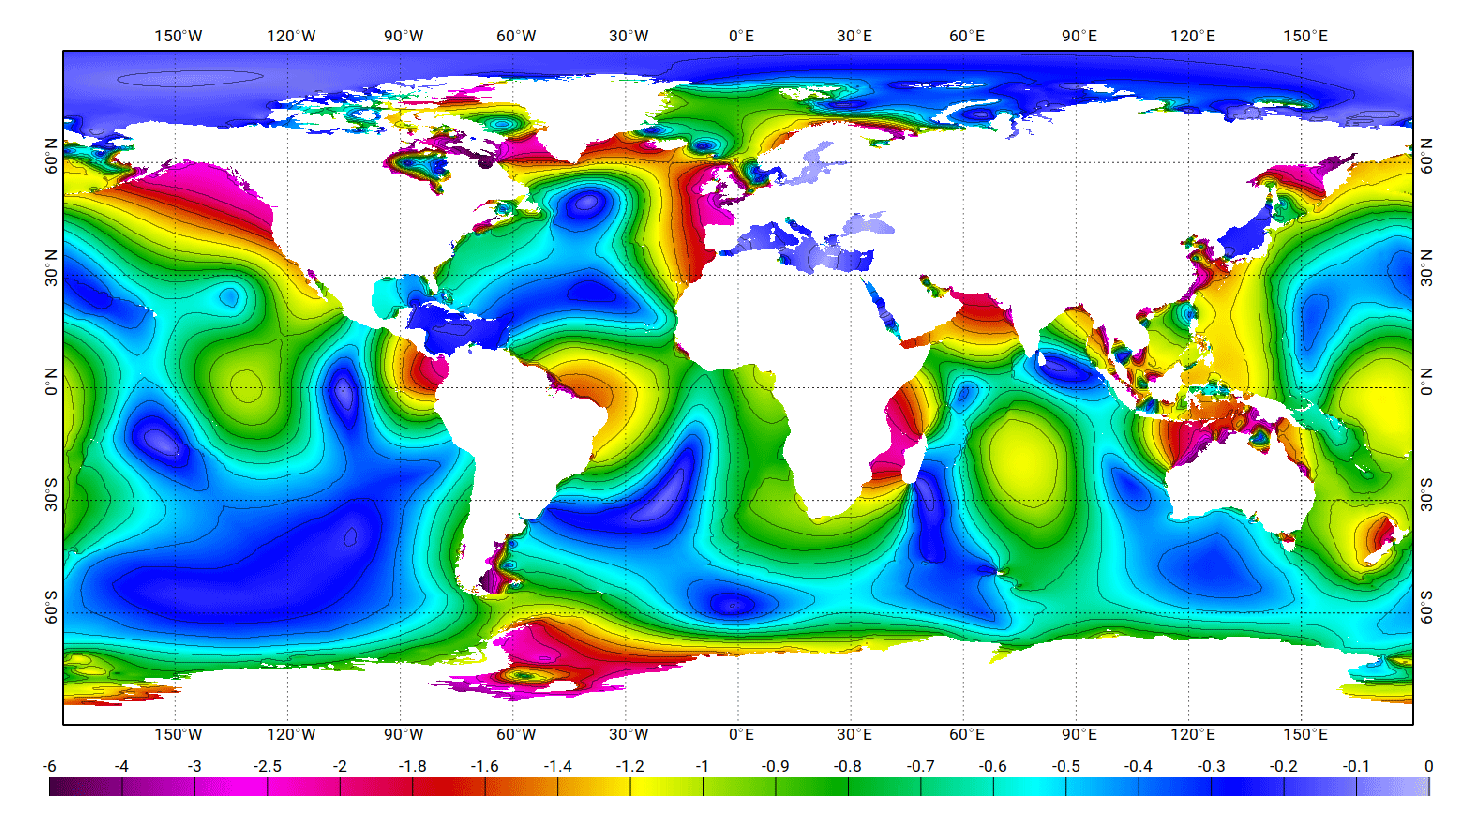
\includegraphics[width=1.1\textwidth]{TidalMaps01.pdf}%
\caption[Amplitude der $M_2$-Tide nach einem numerischen Modell.]{Amplitude f�r die $M_2$-Tide nach einem numerischen Modell \cite{Lyard2021}. Deutlich zu erkennen sind unter anderen die Amphidromiepunkte im Pazifik und im S�datlantik.}
\label{abb:hm_gezeiten06}%
\end{figure}

\begin{figure}%
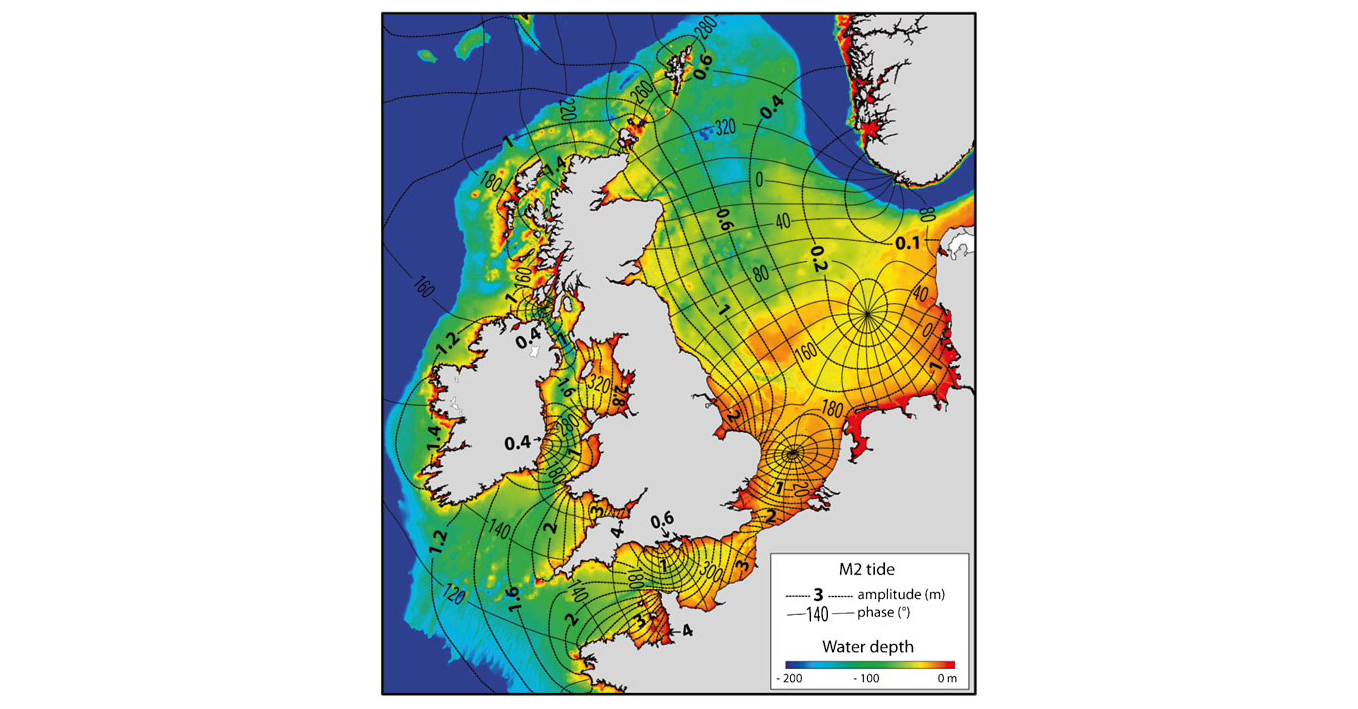
\includegraphics[width=1.2\textwidth]{TidalMaps01a.pdf}%
\caption[Amplitude und Phase der $M_2$-Tide f�r die Nordsee.]{Amplitude und Phase f�r die $M_2$-Tide in der Nordsee mit deutlich erkennbaren Amphidromiepunkten (experimentelle Werte). \cite{Reynaud2012}. Siehe auch \probref{hm_gezeiten03}.}
\label{abb:hm_gezeiten06a}%
\end{figure}

F�r die Seefahrt und andere Anwendungen werden mit gro�em Aufwand Gezeitentafeln publiziert.
Diese beruhen auf der sogenannten harmonischen Analyse von Langzeitbeobachtungen, denen die Annahme zugrunde liegt, dass das Gezeitenverhalten eine �berlagerung von Schwingungen mit Perioden (und Vielfachen der Perioden) von Mond und Sonne darstellt.
Diese periodischen Abh�ngigkeiten sind �berall auf der Welt gleich.
Nur die Einzelphasen und Einzelamplituden (und D�mpfungen) der entstehenden Schwingungen unterscheiden sich von Standort zu Standort.
Heute kann man mit \ca 20--40 der dominanten harmonischen Komponenten (die st�rksten sind die halbt�gliche Mondtide $M_2$ und die halbt�gliche Sonnentide $S_2$) schon sehr gute Vorhersagen machen, da ohnehin die �berlagerung durch lokale Effekte wie Wind, Luftdruck, Erw�rmung, Str�mungs�nderungen Vorhersagen von genauer als auf einen Zentimeter wenig sinnvoll sind. Man beschr�nkt sich daher auf Zentimeter-Genauigkeit.\footnote{Vor dem Aufschwung der digitalen Rechentechnik wurden Gezeitenvorhersagen mit imposanten mechanischen Rechnern durchgef�hrt, heute nat�rlich auf \textit{High-Performance Computern} (HPC).
Selbst auf dem PC kann man heute schon sinnvolle Berechnungen anstellen.}\\
Nachdem wir die Physik der Gezeiten auf der Erde nach den beiden Grundmodellen behandelt haben, wollen wir testen, wie die Ergebnisse mit realen Messungen �bereinstimmen.
Wegen der genannten Komplexit�t und geographischen Besonderheiten ist nicht zu erwarten, dass brauchbare Ergebnisse aus den einfachen theoretischen Rechnungen \zb f�r die Nordsee oder die Atlantikk�ste erzielt werden k�nnen.
Wir haben uns daher die Gezeitentafel in der N�he des �quators f�r Diego Garcia im Indischen Ozean f�r eine �bung herausgesucht (\probref{hm_gezeiten06}), um die Theorie zumindest ansatzweise �berpr�fen zu k�nnen.
Zur Vertiefung dieses komplexen Themas empfehlen wir \ua die Referenzen \cite{Butikov2001, Butikov2014, Weyer2012, Melchior1966, Norsen2017}.

\subsection{Gezeitenreibung}\label{kap:hm_gezeitenreibung}\index{Gezeitenreibung}

\subparagraph{\textbf{Ph�nomenologische Betrachtung}}

In \probref{hm_erdrotation} hatten wir untersucht, wie man aus den Beobachtungsdaten von Sonnenfinsternissen �ber mehrere tausend Jahre schlie�en  kann, dass sich die Erdrotation verlangsamt, \dh die Rotationsperiode $T_\text{P,E}$ gr��er wird.
Es gilt heute als gesichert, dass die Zunahme der Tagesl�nge der Erde etwa $\SI{2.1}{\milli\second}/\mathrm{Jh.}$ betr�gt, was einer Abnahmerate der Rotationsenergie der Erde von 
	\[\frac{\D T_\text{Rot}}{\D t} = \frac{\D}{\D t} \lk\frac{J_\text{E}}{2}\omega^2\rk = \SI{-3.6e12}{\W}
\]
entspricht.
Diese �nderung der Rotationsenergie und des damit verbundenen Drehimpulses muss durch ein Drehmoment der Gr��e
	\[M_\text{D} = \frac{\D}{\D t} \lk {J_\text{E}}\,\omega_\text{E} \rk = \SI{-5.2e16}{\N\metre}\,
\]
hervorgerufen werden \cite{Brosche1989}.
Die ersten Betrachtungen zur Gezeitenreibung gehen auf Halley\indexp{Halley, Edmund} zur�ck.
Immanuel Kant erkannte 1754 als erster die bremsende Wirkung der Meeresgezeiten, jedoch ohne den Zusammenhang zum Mond zu sehen.\indexp{Kant, Immanuel}\footnote{Immanuel Kant (1724 -- 1804) war ein deutscher Philosoph und Professor f�r Logik an der Universit�t K�nigsberg.
Er z�hlt zu den bedeutendsten Philosophen der Geschichte. Mit seiner "`Kritik der reinen Vernunft"' markierte er den Beginn der modernen Philosophie.} Die erste qualitativ richtige Beschreibung lieferte 1848 Robert Mayer%
\indexp{Mayer, Julius Robert von}\footnote{Julius Robert von Mayer (1814 -- 1878) war ein deutscher Arzt und Naturforscher. Er formulierte als einer der ersten Wissenschaftler den Ersten Hauptsatz der Thermodynamik.}, w�hrend 
George Howard Darwin%
\footnote{Sir George Howard Darwin (1845 -- 1912) war ein britischer Astronom und Mathematiker. Er war ein Sohn des ber�hmten Naturforschers Charles Darwin und ist bekannt f�r seine Abspaltungstheorie, nach der der Mond einst Teil der Erde gewesen sein soll.} die Anerkennung f�r die erste vollst�ndige analytische Beschreibung des Problems geb�hrt.\indexp{Darwin, Sir George Howard}\\
Wir werden zun�chst eine einfache ph�nomenologische Beschreibung f�r die Gezeitenreibung geben. Daraus werden wir ein Modell entwickeln, auf dessen Basis wir eine mathematisch-analytische Beschreibung angehen. %, die durchaus mit dem uns zur Verf�gung stehenden mathematisch-physikalischen Instrumentarium m�glich ist.
Wir werden dabei der Einfachheit halber die Gezeitenwirkung der Sonne vernachl�ssigen und nur die Wechselwirkung mit dem Mond in Betracht ziehen.\\
Wir hatten bisher nur �ber die Wirkung der Gezeitenkr�fte auf die Ozeanh�lle gesprochen.
Aber nat�rlich wirken diese auch auf den festen Erdk�rper, der eine gewisse Elastizit�t hat.
Daher wird der Erdk�rper ebenfalls mit phasenverschobenen Oszillationen (seismischen Wellen) auf die Anregung durch die Gezeitenkr�fte antworten, wobei im Gegensatz zu den Ozeanwellen die Eigenfrequenz und die D�mpfung der seismischen Wellen deutlich gr��er sind.
In \kap{hm_gezeiten_Laplace} und \probref{hm_gezeiten05} hatten wir gesehen, dass die �berlagerung dieser Wellen, abh�ngig von deren Eigenfrequenz und D�mpfung zur Ausbildung einer stehenden Welle f�hrt, deren Maximum um einen Winkel $\delta$ phasenverschoben zur Erdmittelpunkt-Mond-Linie ist.
Dabei kommt es im Fall der Erde zu einem vorauseilenden Gezeitenberg ($\delta >0 \approx 3\degree$) (\figref{hm_gezeiten07}).

\begin{figure}%
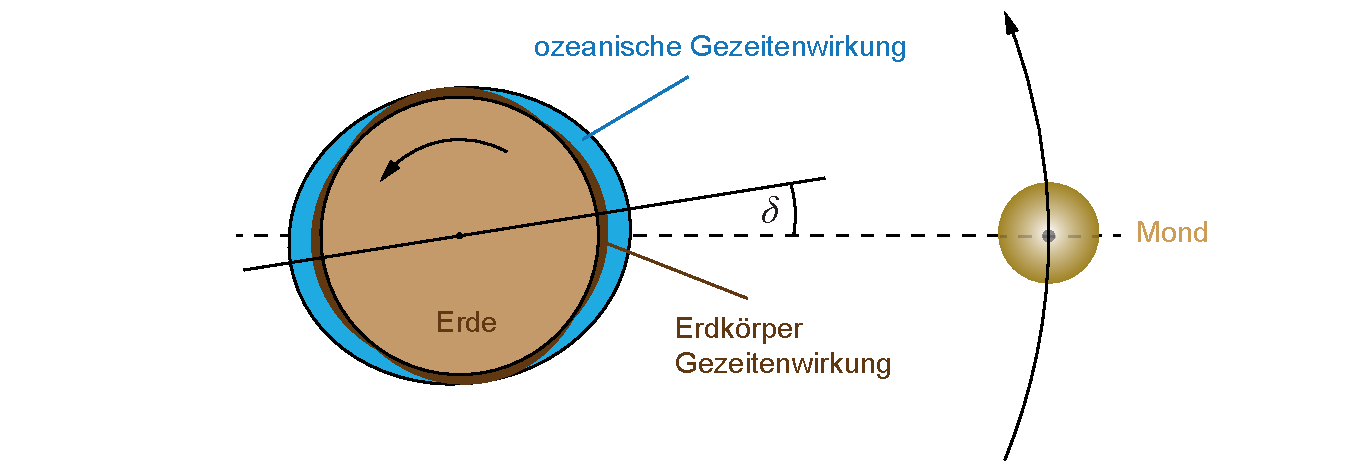
\includegraphics[width=\textwidth]{GezeitenFestOzean.pdf}%
\caption[Gezeitenausbildung im Ozean und im Erdk�rper.]{Gezeitenausbildung im Ozean und im Erdk�rper.}
\label{abb:hm_gezeiten07}%
\end{figure}

Diese von Null verschiedene Phasenlage von Gezeitenberg und Erde-Mond-Linie ist entscheidend f�r das Auftreten von Gezeitenreibung.
Ein vorauseilender Gezeitenberg beschleunigt dabei den Mond und verringert die Erdrotation.
Das kann man sich leicht an \figref{hm_gezeiten08}a klar machen.
Versteht man den Gezeitenberg als Hantel mit Massen an den Punkten A und B, so wird der Mond durch diese in Richtung Hantelkopf A gezogen, also beschleunigt, mithin $\dot{\omega}_\text{M} > 0$.
Da der Effekt im Perig�um \glslink{periapsis} (Erdn�he) am gr��ten ist wird sich auch die Exzentrizit�t der Bahn vergr��ern und folglich $\dot{\omega}_\text{E} < 0$ sein. 
Entsprechend umgekehrt sind die Verh�ltnisse bei einem nachlaufenden Gezeitenberg wie in \figref{hm_gezeiten08}b gezeigt.
Hier wird der Mond ebenfalls in Richtung Hantelkopf A gezogen, mithin verz�gert, folglich ist $\dot{\omega}_\text{M} < 0$ und $\dot{\omega}_\text{E} > 0$. Dabei gilt aber, dass der  die der Gesamtdrehimpuls des Erde-Mond-Systems bleibt erhalten bleibt.
Es ist auch sofort einsichtig, dass es f�r $\delta=0$ keine Beschleunigung oder Verz�gerung geben kann, da das Drehmoment auf Grund der Symmetrie verschwindet.
Entscheidend f�r das Auftreten der Gezeitenreibung ist also ein zeitlicher Versatz des Maximums der Gezeitenellipse zum Meridiandurchgang des Mondes.
Im Fall der Erde f�hrt wie bereits erw�hnt dieser Versatz von \ca $3 \degree$  zu einer experimentell, \zb durch Laserentfernungsmessungen, nachgewiesenen Zunahme des Mondbahnradius von
\begin{equation*}
  \D a_\text{EM}/\D t \approx \SI{4.4}{\cm}/\text{Jahr}\; ,
\end{equation*}
wie wir auch gleich (und auf anderem Weg in \probref{hm_gezeiten06}) nachrechnen wollen.
F�r das Gesamtsystem ist aber keineswegs mechanische Energieerhaltung gegeben, nur ein kleiner Teil (ca. $3\%$) wird von der Mondbahn aufgenommen, der Rest muss in der Erde dissipiert werden.
Wie genau das passiert, ist immer noch ein aktueller Forschungsgegenstand in der Geophysik. 

\begin{figure}%
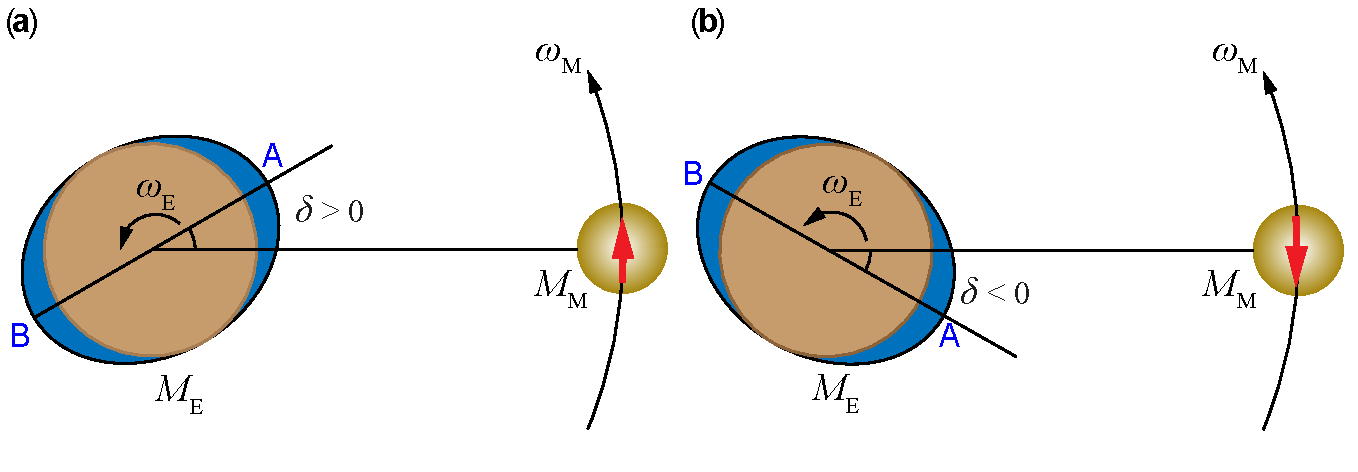
\includegraphics[width=\textwidth]{GezeitenDelay.pdf}%
\caption[Prinzip der Gezeitenreibung.]{Prinzip der Gezeitenreibung. \fa vorlaufender Gezeitenberg, \fb
  nachlaufender Gezeitenberg.}
\label{abb:hm_gezeiten08}%
\end{figure}

\subparagraph{\textbf{Mathematische Beschreibung}}

Wir wollen nun die mathematische Beschreibung angehen.
Das Drehmoment, das vom Mond auf das Gezeitenellipsoid der Erde wirkt, hat als Pendant ein vom Betrag her gleich gro�es aber mit entgegengesetztem Vorzeichen versehenes Drehmoment, das vom Gezeitenellipsoid auf den Mond wirkt.
Dies ist eine direkte Folge der Gesamtdrehimpulserhaltung im Erde-Mond-System. 
Aus dem Winkelversatz $\delta$ berechnet sich ein zeitlicher Versatz $\Delta t =\SI{12}{\minute}$.
%\begin{align}
	%\delta = 360\degree\,\frac{\Delta t}{\SI{24}{\hour}} = 3\degree\,. \label{eq:hm_gezreibung01}
%\end{align}
F�r unsere Rechnungen treffen wir noch einige weitere vereinfachende Annahmen:
\begin{itemize}
   \item Wir vernachl�ssigen, dass der Schwerpunkt des Erde-Mond-Systems um ca. $\SI{4900}{\km}$ vom Erdmittelpunkt verschoben ist und nehmen den Erdmittelpunkt als Zentrum der Mondumlaufbahn.
   \item Der Mond bewegt sich auf einer Kreisbahn mit Radius $a_\text{EM}$ um die Erde.
   \item Der Umlauf des Mondes erfolge in der �quatorebene der Erde und nach dem 3. Keplerschen Gesetz mit der Umlauffrequenz
    \begin{align}
        \omega_\text{M} = \sqrt{\frac{G\,\lk m_\text{E} + m_\text{M}\rk}{a_\text{EM}{}^3}} \,. \label{eq:hm_gezreibung02}
    \end{align}
   \item F�r die gew�hlte Anordnung kann die mit Ozeanen bedeckte Erde ohne Gezeiten als Kugel (Radius $R_\text{E}$) angenommen werden.
   \item Die Erde rotiert mit $\omega_\text{E} =2\pi/T_\text{P,\,E}$.
\end{itemize}
Wir wollen die Wechselwirkung des Gezeitenellipsoids mit dem Mond �ber das Gravitationspotential der Erde (inklusive des Potentials des Gezeitenellipsoids) beschreiben.
In \kap{hm_pot_special cases} \bzw \probref{hm_gezeiten07} hatten wir das Gravitationspotential eines homogenen Rotationsellipsoids berechnet (Gl. \eqref{eq:hm_pot_theo12}). Das k�nnen wir hier verwenden und schreiben bei bekannter Elliptizit�t $\varepsilon$ das Potential dieses durch die Geitenwirkung des Mondes geformten Rotationsellipsoiden folgenderma�en: 
\begin{align}
    U\lk r,\theta\rk = -\frac{G\,M}{r} + \frac{2}{5}\,\varepsilon\,\frac{G\,M\,R^2}{r^3}\,\mathcal{P}_2 \lk\theta\rk  + \mathcal{O}\lk \varepsilon^2\rk \,. \label{eq:hm_gezreibung03a}
\end{align}
Auf die Erde angewandt, bei der die Achse des Rotationsellipsoids um $\delta$ gegen die Erde-Mond-Linie verdreht ist, muss man $\theta$ durch $\theta - \delta$ ersetzen und erh�lt:
\begin{align}
    U\lk r,\theta,\delta\rk = -\frac{G\,m_\text{E}}{r} + \frac{2}{5}\,\hat{\varepsilon} \,\frac{G\,m_\text{E}\,R_\text{E}{}^2}{r^3}\,\lk \frac{3}{2}\cos^2\lk \theta-\delta\rk-\frac{1}{2}\rk \;, \label{eq:hm_gezreibung04}
\end{align}
wobei wir hier mit $\hat{\varepsilon}$ eine allgemeinere Elliptizit�t eingef�hrt haben, die die gesamte elliptische Verformung der Erde durch die Gezeitenkr�fte des Mondes unter Ber�cksichtigung einer teilelastischen Erde beschreibt. 
F�r einen festen K�rper mit einer effektiven Festigkeit\footnote{Die effektive Festigkeit ist eine dimensionslose Gr��e, die sich f�r einen homogenen K�rper aus den Materialeigenschaften berechnen l�sst und f�r die Erde $\approx 3.35$ betr�gt \cite{Fitzpatrick2022}.} $\tilde{\mu}$ findet man \cite{Fitzpatrick2022}:
\begin{align}
\begin{split}
    \hat{\varepsilon}  &= - \frac{15}{4}\,\frac{1}{1+\tilde{\mu}}\, \frac{R_{E}{}^3}{r^3}\,\frac{m_\text{M}}{m_\text{E}} = - \frac{15}{4}\,k\, \frac{R_{E}{}^3}{r^3}\,\frac{m_\text{M}}{m_\text{E}}\,.
\end{split} \label{eq:hm_gezreibung04a}
\end{align}
F�r einen idealen Ozean (mit Dichte 0) hatten wir mit \eqref{eq:hm_gezeiten_epsilon})
\begin{align}
    \hat{\varepsilon}  = -\varepsilon = - \frac{3}{2}\, \frac{R_{E}{}^3}{r^3}\,\frac{m_\text{M}}{m_\text{E}} \label{eq:hm_gezreibung04b}
\end{align}
hergeleitet. Hier haben wir �ber die sogenannte effektive Festigkeit des Planeten $\tilde{\mu}$ etwas vereinfachend die die sogenannte Love\index{Love-Zahl}\footnote{Augustus Edward Hough Love (1863 -- 1940) war ein britischer Mathematiker und Physiker, der besonders auf der Elastizit�tstheorie arbeitete.}\indexp{Love, Augustus Edward Hough}-Zahl $k$ ber�cksichtigt. Sie ist ebenfalls ein dimensionsloser Parameter und ein Ma� f�r die Festigkeit eines K�rpers in Reaktion auf eine Gezeitenkraft und h�ngt von Faktoren wie der Viskosit�t\index{Love-Zahl}\index{Viskosit�t} (siehe Kapitel 2 Band I) und der Reibung ab. Sie ist ein Ausdruck daf�r, dass sich der Gezeitenberg  nicht bis zu seiner theoretisch maximal m�glichen H�he ausbilden wird. Die beiden Gleichungen \eqref{eq:hm_gezreibung04a} und \eqref{eq:hm_gezreibung04b} zeigen im Vergleich, dass die Gezeitenwirkung auf einer teileastischen Erde das $\frac{5}{2} k$-fache der Wirkung auf einen (idealen, masselosen) die Erde umspannenden Ozean betragen. Wir rechnen im Folgenden f�r die Erde  mit einer Love-Zahl $k$ im Bereich von 0.2.

Dann ist das Gravitationspotential des herausgebildeten Rotationsellipsoids der teilelastischen Erde (wir rechnen im weiteren nur mit diesen Werten), das auf den Mond wirkt, gegeben durch:
\begin{align}
    U\lk r,\theta,\delta\rk &= -\frac{G\,m_\text{E}}{r}-\frac{2}{5}\,\frac{15}{4}\,k\,\frac{G\,m_\text{M} \,R_{E}{}^5}{r^6}\,\mathcal{P}_2 \lk\cos(\theta - \delta) \rk \nonumber \\
														&= -\frac{G\,m_\text{E}}{r}-\frac{3}{2}\,k\,\frac{G\,m_\text{M} \,R_{E}{}^5}{r^6}\, \lk \frac{3}{2}\cos^2\lk\theta-\delta\rk - \frac{1}{2}\rk \,.  \label{eq:hm_gezreibung05}
\end{align}
Durch dieses Potential, oder besser gesagt die daraus folgende Kraft, wird ein Drehmoment auf den Mond ausge�bt, was sich in sph�rischen Koordinaten berechnet zu:
\begin{align}
\begin{split}
    \vec{M}_\text{D} &= \vec{r} \times \vec{F}  = - m_\text{M}\,  \vec{r} \times \vec{\nabla}{U} = - m_\text{M}\,\frac{1 \,\d U}{r \,\d \theta} \,r \,\,\vec{e}_r \times \vec{e}_\theta \\
										 &= - m_\text{M}\,\frac{\d U}{\d \theta} \vec{e}_\phi\, |_{\theta=0,r=a_\text{EM}} \,. \label{eq:hm_gezreibung06}
\end{split}
\end{align}
F�r den Betrag des Drehmoments erhalten wir: 
\begin{align}
    \left|\vec{M}_\text{D}\right|  & \approx \frac{9}{2}\,k\,\delta \,\frac{G\,m_\text{M}{}^2}{R_\text{E}}\,\lk \frac{R_\text{E}}{a_\text{EM}}\rk^6\,, \label{eq:hm_gezreibung07} 
\end{align}
wobei wir kleine Winkel angenommen haben ($\sin\delta\approx \delta, \cos\delta\approx 1$). \\
Wie bereits erw�hnt, gibt es nur f�r $\delta\neq 0$ ein Drehmoment.
Wir finden nun die eingangs gemachte �berlegung, wie das Drehmoment wirkt, best�tigt, ein $\delta > 0$ bewirkt eine Beschleunigung des Mondes (und damit eine Verlangsamung der Erdrotation), f�r $\delta<0$ umgekehrt (siehe auch \probref{hm_gezeiten06}).\\
Wir wollen jetzt noch die Gr��enordnungen der Effekte der Gezeitenreibung absch�tzen.
Wir wissen, dass das Drehmoment eine �nderung des Drehimpulses bewirkt.
Da (wie angenommen) die Bewegung in einer Ebene stattfindet, kann sich nur der Betrag des Drehimpulses �ndern.
Wir schreiben f�r die �nderung des Betrages des Erddrehimpulses:
\begin{align}
    \frac{\D}{\D t} L_\text{E} &= \frac{\D}{\D t} (J_\text{E}\,\omega_\text{E}) = - \left|\vec{M}_\text{D}\right|  \,, \nonumber \\ 
		\rightarrow~~\dot{\omega}_\text{E} &= - \frac{\left|\vec{M}_\text{D}\right|}{J_\text{E}} = - \frac{45}{4}\,\frac{G\,m_\text{M}{}^2}{m_\text{E}}\,\frac{R_\text{E}{}^3}{a_\text{EM}{}^6}\,k\,\delta\,.
		\label{eq:hm_gezreibung07a}
\end{align}
Mit dem 3. Keplerschen Gesetz \eqref{eq:hm_gezreibung02} finden wir schlie�lich:
\begin{align}
    \frac{\dot{\omega}_\text{E}}{\omega_\text{E}} &= - \frac{45}{4}\,k\,\delta\,\frac{\omega_\text{M}{}^2}{\omega_\text{E}}\,\frac{m_\text{M}{}^2}{m_\text{E}{}^2}\,\frac{R_\text{E}{}^3}{a_\text{EM}{}^3}\approx \SI{-8e-18}{\per\second}\,.
		\label{eq:hm_gezreibung08}
\end{align}
Mit dieser Abnahmerate der Rotationsgeschwindigkeit erhalten wir eine Verl�ngerung der Rotationsdauer der Erde um
\begin{equation*}
  \Delta T_\text{P,E}=-\frac{\dot{\omega}_\text{E}}{\omega_\text{E}}\,T_\text{PE}\,\,100\, \mathrm{a} \approx \SI{2.17e-03}{\second} \approx \SI{2.2}{\milli\second}
\end{equation*}
pro Jahrhundert.
Die Zeit bis zur synchronen Rotation der Erde betr�gt dann $\Delta T_\text{synch} = \omega_\text{E}/\dot{\omega}_\text{E} \approx \SI{4e+09}{}$ Jahre.\\
Die Drehimpulserhaltung im Erde-Mond-System kann formuliert werden als:
\begin{align}
	L_\text{ges} &=\frac{2}{5}\,m_\text{E}\,R_\text{E}^2\,\omega_\text{E} + m_\text{M}\,a_\text{EM}^2\,\omega_\text{M} = \mathrm{const} \,. \label{eq:hm_gezreibung09}
\end{align}
Ableitung von \eqref{eq:hm_gezreibung09} nach der Zeit und Benutzung von \eqref{eq:hm_gezreibung02} ergibt die Bahnvergr��erungsrate des Mondes zu:
\begin{align}
    \frac{\dot{a}_\text{EM}}{a_\text{EM}} &= -\frac{4}{5}\,\frac{m_\text{E}\, R_\text{E}{}^2}{m_\text{M}\, a_\text{EM}{}^2} \,\frac{\dot{\omega}_\text{E}}{\omega_\text{M}} = C_a  \approx \SI{+3.9e-18}{\per\second} \,, \label{eq:hm_gezreibung10}
\end{align}
was gleichbedeutend mit einer Vergr��erung des Radius der Mondbahn von $ \Delta a_\text{EM} \approx \SI{+4.7}{\metre}$ pro Jahrhundert ist.
Aus der Ableitung von \eqref{eq:hm_gezreibung02} nach der Zeit erh�lt man die Abnahmerate der Umlauffrequenz des Mondes zu $ \dot{\omega}_\text{M}/\omega_\text{M} = -\frac{3}{2}\,C_a \approx \SI{-5.82e-18}{\per\second}$, was wiederum einer Verl�ngerung des synodischen Mondmonats um $\SI{+43}{\milli\second}$ pro Jahrhundert entspricht.\\
Zum Schluss wollen wir noch die Energiedissipation ausrechnen.
Sie ist gleich der vom Drehmoment \eqref{eq:hm_gezreibung07} geleisteten Arbeit pro Zeit:
\begin{align}
   P = \left|\vec{M}_\text{D}\right|\,(\omega_\text{M} - \omega_\text{E}) \approx \SI{-3.90e+12}{\W} \,. \label{eq:hm_gezreibung11}
\end{align}
Die Leistung ist negativ, da $\omega_\text{M} < \omega_\text{E}$ ist.
Sie muss also dissipiert werden.
Die Verlustleistung f�hrt zu einer Erw�rmung der Ozeane und der Erdkruste.
Bei starker Gezeitenreibung, wie sie in anderen Planeten-Mond-Systemen auftritt, kann die Gezeitenerw�rmung zur Verfl�ssigung und vulkanischen Effekten f�hren.
Um ein Gef�hl f�r die Gr��enordnung auf der Erde zu bekommen, geben wir zum Vergleich die gesamte in Deutschland installierte Leistung aller Kraftwerke im Jahre 2022 an: $P_\text{el} = \SI{-2.38e+11}{\W}$ \cite{BNA2022}. Wenn der Zustand der synchronen Rotation erreicht ist, \dh $\omega_\text{M} = \omega_\text{E}$ ist, gibt es auch keine Energiedissipation mehr. 
Alle Berechnungen finden sich im Detail im \mscr{} \mlhmref{Gezeitenreibung01.m}.\\

\subparagraph{\textbf{L�sung der Bewegungsgleichungen}}

Wir wollen jetzt noch kurz beschreiben, wie man das Erde-Mond-System inklusive Gezeitenreibung in seiner zeitlichen Entwicklung numerisch berechnen kann.
Das ist aber nicht ganz so einfach.\footnote{Siehe auch dazu \cite{Schebesta1994}.} Bisher hatten wir die Verdrehung $\delta$ der Gezeitenh�lle als konstant angenommen und daraus das Drehmoment berechnet.
In der Zeitentwicklung wird sich aber $\delta$ verringern bis bei $\delta = 0$ der stabile Endzustand, die gebundene Rotation, erreicht ist.
Das bedeutet, dass das in den Bewegungsgleichungen auftretende Drehmoment von den �ber lange Zeitr�ume sich relativ zueinander ver�ndernden Positionen der Himmelsk�rper abh�ngig ist.
Um die Bewegungsgleichungen f�r Erde und Mond zu erhalten, bilden wir den Gradienten aus dem Potential \eqref{eq:hm_gezreibung05}, das wir als 
	\[U = U_\text{G} + U_\text{Ell}	\,\]
schreiben. Wir benutzen die Koordinatensysteme nach \figref{hm_gezeiten09}.
Der Gradient $\vec{\nabla}_{\vec{r}_\text{E}} U_\text{G}$ erzeugt die Monopolkraft, die auf den Mond wirkt:
\begin{align}
    \vec{F}_\text{G}' \lk \vec{r}_\text{M}'\rk = -G\,m_\text{E}\,m_\text{M}\,\frac{\vec{r}_\text{E}'-\vec{r}_\text{M}'}{|\vec{r}_\text{E}' - \vec{r}_\text{M}'|^3}\,.  \label{eq:hm_gezreibung12}
\end{align}

Bei der L�sung der Bewegungsgleichungen m�ssen wir die Bewegung der beiden Himmelsk�rper um den gemeinsamen Schwerpunkt ber�cksichtigen.
Die mit einem Strich gekennzeichneten Koordinaten sollen  sich auf das Koordinatensystem $\vec{\Sigma}'$ beziehen, dessen Ursprung im gemeinsamen Schwerpunkt der beiden Massen $m_\text{E}$ und $m_\text{M}$ liegt.\footnote{Wir k�nnen die nachfolgenden �berlegungen auch auf ein beliebiges Zweik�rperproblem (Satellit-Zentralk�rper) anwenden, es gilt dann einfach f�r die Indizes E = 1 und M = 2.} Aus dem Potentialanteil der Ellipsoidh�lle $U_\text{Ell}$ berechnet man ebenfalls durch Gradientenbildung die Gezeitenkraft $\vec{F}_\text{Gez}$ die auf den Mond wirkt.
Dabei m�ssen wir beachten, dass die Gezeitenkraft bez�glich des Koordinatensystems $\vec{\Sigma}$ definiert ist, das seinen Ursprung im Massenmittelpunkt der Erde hat (\figref{hm_gezeiten09}).
F�r die Bewegungsgleichungen k�nnen wir aber eine einfache Transformation von $\vec{\Sigma}$ und $\vec{\Sigma}'$ �ber die Translation
\begin{align}
	\vec{r}_\text{M} = \vec{r}_\text{M}' - \vec{r}_\text{E}'  \label{eq:hm_gezreibung12a}
\end{align}
erreichen.
Wir erhalten f�r die Gezeitenkraft im KOS $\vec{\Sigma}$:\\ 
\begin{align}
\vec{F}_\text{Gez}\lk \vec{r}_\text{M}\rk &= m_\text{M}\,\lk -\vec{\nabla}_{\vec{r}_\text{E}}\,U_\text{Ell}\lk \vec{r}_\text{M}\rk\rk \nonumber \\
&= \frac{3}{10}\,k\,G\,m_\text{M}{}^2\,\frac{R_\text{E}^5}{r_\text{M}^*{}^5}\,\lek \frac{6\,\lk \vec{r}_\text{M}^*\cdot \vec{r}_\text{M}\rk}{r_\text{M}{}^5}\vec{r}_\text{M}^* - \lk \frac{15\,\lk \vec{r}_\text{M}^*\cdot\vec{r}_\text{M}\rk^2}{r_\text{M}{}^7} + \frac{3{r_\text{M}^*}^2}{r_\text{M}{}^5}\rk\,\vec{r}_\text{M}\rek \,. \label{eq:hm_gezreibung13}
\end{align}

\begin{figure}%
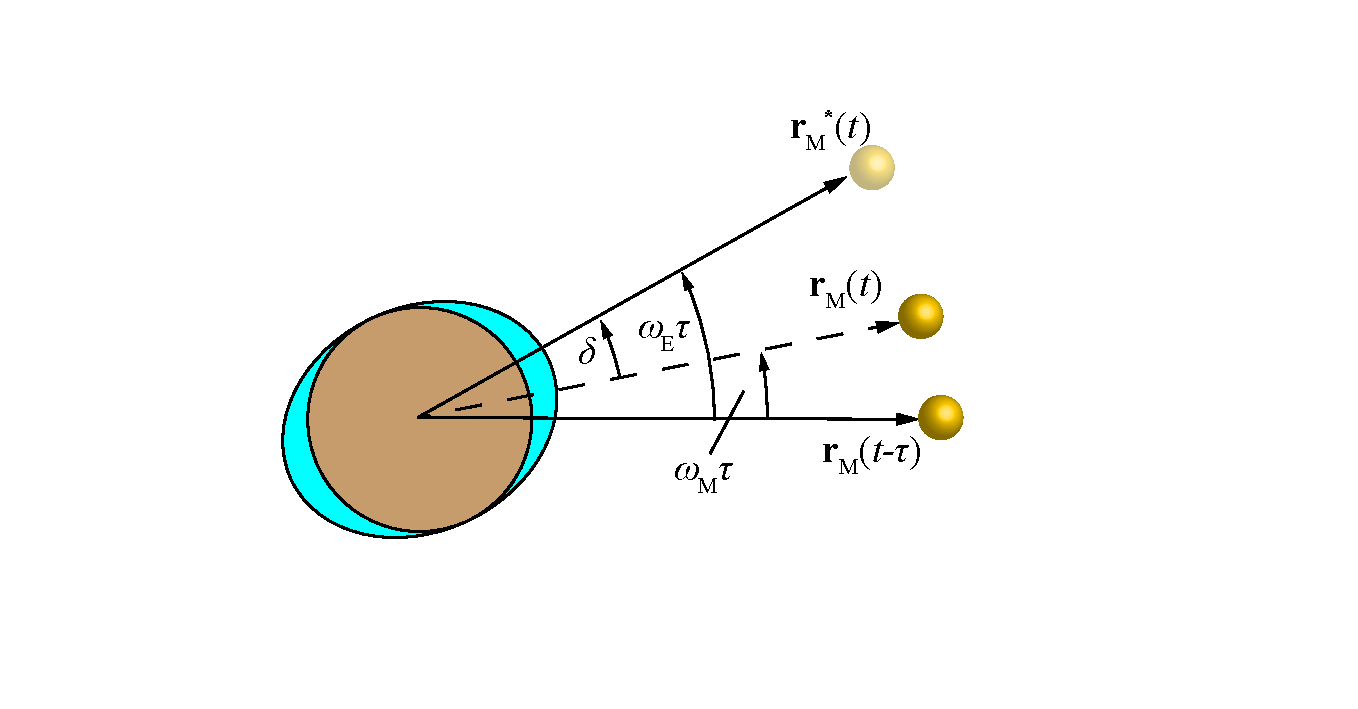
\includegraphics[width=\textwidth]{KOSGezeitenreibung.pdf}%
\caption[Koordinatensysteme der Bewegungsgleichungen der Gezeitenreibung.]{Mitrotierendes Koordinatensysteme $\vec{\Sigma}$ f�r numerische L�sung der Bewegungsgleichungen der Gezeitenreibung zu einer Zeit $t$. Der virtuelle Mond steht im Zenit �ber dem Hochwasser-Berg $\vec{r}_\text{M}^*$, $\vec{r}_\text{M}(t-\tau)$ ist der Ort, an dem ein mitrotierender Beobachter den Mond zur Zeit $t-\tau$ im Zenit gesehen hat. Inzwischen, zur Zeit $t$, befindet sich der Mond aber am Ort $\vec{r}_\text{M}$.}
\label{abb:hm_gezeiten09}%
\end{figure}

Hier haben wir nun einen neuen Vektor eingef�hrt: $\vec{r}_\text{M}^*$. Dies ist der Vektor zum Mond, als dieser kulminierte (\figref{hm_gezeiten09}) oder m.a.W. der Ort des Mondes zu einem Zeitpunkt, als dieser die Gezeitendeformation hervorrief.
Dieser Ort ist aber aufgrund der zeitverz�gerten Antwort der Erde auf die Gezeitenkraft nicht mit dem gegenw�rtigen Ort des Mondes $\vec{r}_\text{M}$ identisch.
Diese Zeitverz�gerung hatten wir mit dem Winkel $\delta \propto \Delta t $ %\eqref{eq:hm_gezreibung01} 
beschrieben.
W�hrend dieser Zeit $\Delta t $ dreht sich die Erde mit $\omega_\text{E}$ um ihre Achse und der Mond mit $\omega_\text{M}$ um die Erde.
Der Zenitalpunkt Z bewegt sich f�r einen Beobachter auf dem  Planeten - im mitrotierenden Koordinatensystem - mit der Winkelgeschwindigkeit $\omega_\text{M} - \omega_\text{E}$.
Wir k�nnen $\vec{r}_\text{M}^*$ auch als die Position eines virtuellen Mondes bezeichnen, der einen instantanen Gezeitenberg erzeugen w�rde.
Der Winkel $\delta$ ist �ber das Skalarprodukt
\begin{align*}
    \vec{r}_\text{M}\cdot\vec{r}_\text{M}^* = |\vec{r}_\text{M}|\,|\vec{r}_\text{M}^*|\,\cos\delta\,.
\end{align*}
mit den beiden Vektoren $\vec{r}_\text{M}$ und $\vec{r}_\text{M}^*$  verkn�pft, die beide im mitrotierenden KOS $\vec{\Sigma}$ definiert sind.

Auf den Schwerpunkt des Mondes wirkt die Summe der Kr�fte $\vec{F}_\text{G}'$ und $\vec{F}_\text{Gez}'$, die Newtonschen Bewegungsgleichungen lauten:
\begin{align}
    m_\text{M}\,\ddot{\vec{r}}_\text{M}' = \vec{F}_\text{G}' + \vec{F}_\text{Gez}'\,. \label{eq:hm_gezreibung14}
\end{align}
Entsprechend gilt f�r den Schwerpunkt der Erde nach dem 3. Newtonschen Axiom:
\begin{align}
    m_\text{E}\,\ddot{\vec{r}}_\text{E}' = -\vec{F}_\text{G}' - \vec{F}_\text{Gez}'\,. \label{eq:hm_gezreibung15}
\end{align}
Wir hatten gesehen, dass die Gezeitenkraft als (r�cktreibendes Moment) auf die Gezeitenh�lle der Erde wirkt.
Die daraus folgende Drehimpuls�nderung wird beschrieben durch:
\begin{align}
    \frac{\D \vec{L}}{\D t} = C\,\dot{\omega}\,\vec{e}_z = -\lk \vec{r}_\text{M} \times \vec{F}_\text{Gez}\rk  
		= \lk r_{\text{M}\,y} \,F_{\text{Gez}\, x}- r_{\text{M}\, x}\,F_{\text{Gez}\, y} 	\rk \,\vec{e}_z  \,. \label{eq:hm_gezreibung16}
\end{align}
Hier haben wir von der Annahme Gebrauch gemacht, dass alle Bewegungen in der $x$-$y$-Ebene stattfinden sollen.%
\footnote{Tats�chlich sind durch die Rotationsabplattung der Planeten (\vgl �bung 1.17 in Band I) die meisten Monde und Kleink�rper in unserem Sonnensystem in unmittelbarer N�he der �quatorebene anzutreffen.}
Mit \eqref{eq:hm_gezreibung10} bis \eqref{eq:hm_gezreibung12} haben wir nun ein Differentialgleichungssystem vorliegen, das uns erlaubt, die zeitliche Entwicklung des Erde-Mond-Systems unter Ber�cksichtigung der Gezeitenreibung zu beschreiben.
Um auch wirklich die Reibung der Gezeiten zu beschreiben, erg�nzen wir die Differentialgleichungen durch einen Reibungsterm proportional zur Geschwindigkeit.
Mit \eqref{eq:hm_gezreibung12a} erhalten wir:
\begin{align}
\begin{split}
    \ddot{r}_{\text{M}\, x}' &= \frac{1}{m_\text{M}}\,\lk   F_{\text{G}\, y}' + F_{\text{Gez}\, x}' - \beta\,|\vec{r}_\text{M}'|\,\dot{r}_{\text{M}\, x}'\rk \,, \\
    \ddot{r}_{\text{M}\, y}' &= \frac{1}{m_\text{M}}\,\lk   F_{\text{G}\, y}' + F_{\text{Gez}\, y}' - \beta\,|\vec{r}_\text{M}'|\,\dot{r}_{\text{M}\, y}'\rk \,, \\
    \ddot{r}_{\text{E}\, x}' &= \frac{1}{m_\text{E}}\,\lk - F_{\text{G}\, x}' - F_{\text{Gez}\, x}' - \beta\,|\vec{r}_\text{E}'|\,\dot{r}_{\text{E}\, x}'\rk \,, \\
    \ddot{r}_{\text{E}\, y}' &= \frac{1}{m_\text{E}}\,\lk - F_{\text{G}\, y}' - F_{\text{Gez}\, y}' - \beta\,|\vec{r}_\text{E}'|\,\dot{r}_{\text{E}\, y}'\rk \,, \\
    \dot{\omega}_\text{E} &= \frac{1}{C}\,\lek \lk r_{\text{M}\,y}'-r_{\text{E}\, y}'\rk\,F_{\text{Gez}\, x} - \lk r_{\text{M}\,x}' - r_{\text{E}\,x}'\rk\,F_{\text{Gez}\, y}\rek \,.
\end{split} \label{eq:hm_gezreibung17}
\end{align}
In den $\vec{F}_\text{Gez}$ \bzw $\vec{F}_\text{Gez}'$  finden wir die Koordinate $\vec{r}_\text{M}^*(t)$.
Die Frage ist, wie man sich diese Koordinate f�r die numerischen Rechnungen beschafft.
Aus Abbildung \figref{hm_gezeiten09} erkennt man, dass f�r ann�hernd kreisf�rmige Bahnen gilt:
\begin{align}
    \vec{r}_\text{M}^*(t) = \mathbb{R}_z(\omega_\text{E}\,\tau)\, \vec{r}_\text{M}(t-\tau) \,, \label{eq:hm_gezreibung18}
\end{align}
worin $\mathbb{R}_z$ die Rotationsmatrix um die $z$-Achse ist.
Im numerischen Programm muss man also eine Routine haben, die alle Orte speichert, an denen der Mond war.
Die numerische Integration von \eqref{eq:hm_gezreibung17} selbst erfolgt aber im raumfesten Schwerpunktsystem $\vec{\Sigma}'$ �ber die Vektoren $\vec{r}_\text{M}'$ und $\vec{r}_\text{E}'$.
Mit der Transformation \eqref{eq:hm_gezreibung12a} und \eqref{eq:hm_gezreibung17} k�nnen wir uns alle Orte $\vec{r}_\text{M}^*(t)$ berechnen und abspeichern, die wir zur numerischen L�sung von 
\eqref{eq:hm_gezreibung17} brauchen.
%Wir geben Hinweise zur relativ komplexen numerische Berechnung in \probref{hm_gezeiten08} an.\\

Mit der Berechnung von Sonnenfinsternissen und der Gezeiten, insbesondere der Gezeitenreibung haben wir so etwas wie die \anf{h�here Schule der Himmelsmechanik} absolviert.
In \figref{hm_gezeiten10} geben wir noch einmal einen graphischen �berblick �ber die wesentlichen Effekt der Mechanik auf unsere Erde.
Es wichtig bei diesen die jeweiligen wirkenden Kr�fte und Koordinatensysteme auseinander zu halten, siehe dazu auch \probref{hm_gezeiten09}.

\begin{figure}[H]
	\includegraphics[width=\textwidth]{VergleichEffekte.pdf} 
	\caption[Vergleich verschiedener Effekte der Himmelsmechanik auf unsere Erde.]{Vergleich verschiedener Effekte der Himmelsmechanik auf unsere Erde. \fa Rotationsabplattung der Erde durch Zentrifugalkraft \fb Pr�zession der Erdachse durch Drehmoment von Mond und Sonne auf die "`�quatorw�lste"' der Rotationsabplattung \fc Gezeitenformation nach der Gleichgewichtstheorie \fd Gezeitenreibung durch Drehmoment des Mondes auf die verdrehte "`Gezeitenh�lle"'.}
	\label{abb:hm_gezeiten10}
\end{figure}



\section{Himmelsmechanik unseres Sonnensystems �ber lange Zeitr�ume}\label{kap:hm_langezeiten}

\subsection{Bahnparameter der Planeten in ihrer zeitlichen Entwicklung}

Bevor wir die Himmelsmechanik endg�ltig verlassen wollen, werfen wir noch einen Blick auf die Entwicklung unseres Sonnensystems �ber lange Zeitr�ume.
Dabei spielen zwei Effekte eine Rolle, zum einen die Ver�nderung der Bahnparameter �ber lange Zeiten, die zu deutlich ver�nderten Konstellationen (z.\,B. Jahreszeiten) f�hren, insgesamt aber noch deterministisch sind. Zum anderen kann es �ber sehr lange Zeiten zur Entstehung von \anf{Chaos} kommen, d.\,h. nicht mehr sicher vorhersagbaren Bahnen und Konstellationen.
Mit dem ersten Ph�nomen wollen wir uns noch kurz besch�ftigen, zum Thema Chaos verweisen wir auf die detaillierten Darstellungen in \cite{Murray2008, Walter2018} oder die sehr unterhaltsame Darstellung in \cite{Peterson1993}.\\
Wir haben bereits mehrfach erw�hnt, dass weder die Erdbahnebene noch die Erdachse und auch nicht die Apsidenlinie\index{Apsidenlinie} fest im Raum liegen, sondern durch Gravitationseinfl�sse der anderen Himmelsk�rper st�ndig ihre Lagen �ndern. Im Kapitel 1.5.5 hatten wir die Frequenz der Pr�zession der Erdachse berechnet.\footnote{F�r eine vertiefte Betrachtung empfehlen wir auch die Ref. \cite{Rainey2022}.}
Man kann und muss daher auch die Bahnelemente als zeitabh�ngig betrachten und jeweils die Angaben zu Epoche und �quinoktium, auf die sich die Bahnelemente beziehen, ber�cksichtigen (\kapitel{hm_raum_und_zeit}).
Starten wir beim Bezugspunkt J2000, dann k�nnen wir die zeitliche Entwicklung der Bahnparameter n�herungsweise durch ein System von Polynomen beschreiben \cite{Montenbruck1999, Meeus1998}
\begin{equation}
x(t) = x_0 + \sum_{k=1}^3 x_k t^k\label{eq:hm_epsilon_schief} \,,
\end{equation}
mit $x\!=\!a$, $e$, $i$, $\Omega$, $\varpi$, $M$, $L$ und $L_0$. Auch die Schiefe der Ekliptik $\epsilon$ unterliegt einer zeitlichen Ver�nderung:
\begin{equation*}
\epsilon(t) = \epsilon_0 + \sum_{k=1}^3 \epsilon_k t^k  \,,
\end{equation*}
mit $\epsilon_0\!=\!23.43929111\degree,\,\epsilon_1\!=\!46.8150'',\,\epsilon_2\!=\!0.00059'',\,\epsilon_3\!=\!0.00181''$.
$t$ ist die Zahl der Julianischen Jahrhunderte seit J2000.
Die linearen Parameter $x_k$ sind in der Tabelle \ref{tab:hm_zeitl_aenderung_bahnparameter_lin} im Anhang zusammengefasst\footnote{F�r die Erde gelten, wie weiter oben vermerkt, die Parameter f�r den Massenmittelpunkt Erde-Mond.}, wobei wir uns wie bisher jeweils auf das �quinoktium des Datums beziehen wollen.\footnote{In der Tabelle \ref{tab:hm_zeitl_aenderung_bahnparameter_lin} sind auch die Parameter f�r das �quinoktium J2000 angegeben.} Die Formeln gelten gut f�r den Zeitraum von 1800 bis 2050.
Wir werden uns gleich noch Formeln anschauen, die wir f�r gr��ere Zeitr�ume verwenden k�nnen. 

\subsection{Berechnungen �ber einen Zeitraum von 10000 Jahren}\label{kap:hm_altertum_zeiten}

Die Frage ist nun, welche m�glichen Konsequenzen neben der offensichtlichen Korrektur der Koordinaten eines Himmelsk�rpers eine solche Ver�nderung der Bahnparameter und der Richtung der Erdachse �ber lange Zeiten hat.
In \probref{hm_erdbahn_im_jahr} sch�tzen wir mit einem einfachen Modell die Ver�nderung der Dauer der Jahreszeiten und des mittleren Sonnenenergieeintrags\index{Sonnenenergieeintrag} pro Zeiteinheit pro Hemisph�re ab.
Das einfache Modell ber�cksichtigt die Pr�zession der Erdachse sowie eine Variation der \gls{exzentr-hm} und der \gls{ekliptikschiefe}.
Wir k�nnen mit dem Modell zeigen, dass sich in einem Zeitraum von ca. 40\,000 Jahren sowohl die Dauer des Sommerhalbjahres als auch der mittlere Energieeintrag pro Zeiteinheit deutlich ver�ndern.
Wir wollen hier noch etwas genauere Rechnungen f�r einen Zeitraum von etwa 1000 n.~Chr.\ bis 8000 n.~Chr.\ machen, was nat�rlich in astronomischen Dimensionen eine unvorstellbar kurze Zeitspanne ist.
Es entspricht aber in etwa der doppelten Zeitspanne, die vergangen ist, seit Menschen in Babylon und �gypten begannen, Astronomie zu betreiben.
F�r diesen Zeitraum sind f�r die Exzentrizit�t $e$, die L�nge des Perihels $\varpi$, sowie die Neigung der Erdachse $\epsilon$ die Parameter f�r die N�herungspolynome in Tabelle \ref{tab:hm_parameter_longtimes} angegeben:

\begin{table}%tab
\caption[Parameter f�r Zeitr�ume von 2000 Jahren.]{Parameter der Elliptizit�t $e$, der Ekliptikneigung $\epsilon$ und der L�nge des Perihels $\varpi$ f�r Zeitr�ume von 2000 Jahren \cite{Meeus1998,Laskar1986}.}
\centering\begin{tabular}{L{1cm}C{4cm}C{2.5cm}C{3cm}}
\hline\noalign{\smallskip}
Ordnung $(t^n)$			&	Ekliptikneigung $\epsilon$ in Bogensekunden ('') \linebreak (wenn nicht anders angegeben)	& Elliptizit�t $e$ & L�nge des Perihels \linebreak $\varpi$ in Grad ($\degree$)  \\
\noalign{\smallskip}\svhline\noalign{\smallskip}
		---				&	$23.439291111\degree$			&	$0.016708634$ 							&$102.9373481$	\\ 
		$t^1$				&	$-4.68093 \cdot 10^{+1}$	&$-4.20365 \cdot 10^{-5} $		&$+1.7194598028 $\\
		$t^2$				&	$-1.55000 \cdot 10^{-4}$	&$-1.26736 \cdot 10^{-7}$		&$+4.56833 \cdot 10^{-4}$	\\
		$t^3$				&	$+1.99925 \cdot 10^{-3}$	&$+1.44400 \cdot 10^{-10}$		&$-1.76800 \cdot 10^{-8}$	\\
		$t^4$				&	$-5.13800 \cdot 10^{-7}$	&$-2.00000 \cdot 10^{-14}$		&$-3.35830 \cdot 10^{-9}$	\\
		$t^5$				&	$-2.49670 \cdot 10^{-8}$	&$+3.00000 \cdot 10^{-15}$		&$+8.28000 \cdot 10^{-12}$	\\
		$t^6$				&	$-3.90500 \cdot 10^{-11}$	&$+0.00000$										&$+5.60000 \cdot 10^{-14}$	\\
\noalign{\smallskip}\hline\noalign{\smallskip}	
\end{tabular}
\label{tab:hm_parameter_longtimes}
\end{table}
Wir wollen mit diesen Parametern die Ver�nderungen in der Zeitgleichung und des Analemmas berechnen, indem wir in \eqref{eq:hm_parameter_alpha_beta} bzw. \eqref{eq:hm_parameter_alpha_beta2} f�r verschiedene Zeiten (1246, 2000 und 8000) die  entsprechend berechneten Bahnparameter einsetzen.
Wir beziehen uns dabei auf das jeweilige �quinoktium des Datums.
Das Ergebnis in \figref{hm_ZGL_Analemma_long} (siehe \mscr{} \mlhmref{ZGL04.m}) zeigt deutlich, wie die relativ geringen Ver�nderungen der Ekliptikneigung und der Exzentrizit�t zu einer Ver�nderung der ZGL und damit des \gls{analemma}s f�hren.
Das Jahr 1246 ist dahingehend interessant, dass die ZGL f�r die beiden Halbjahre perfekt antisymmetrisch ist.
Folglich steht das Analemma genau senkrecht und ist voll symmetrisch.\footnote{Wir wollen bemerken, dass wir bei diesen langen Zeiten auf jeden Fall die Gr��e $\Delta T = \text{UT}- \text{ET}$ zum jeweiligen Zeitpunkt ber�cksichtigen m�ssen.
Nun ist diese Gr��e nur n�herungsweise f�r die Vergangenheit bekannt und f�r die Zukunft bestenfalls durch N�herungsformeln beschreibbar \cite{Espenak2014}.
Wir haben deshalb gesetzt: $\Delta T (1246) = 640\:\text{s} $, $\Delta T (2000) = 64\:\text{s} $ und $\Delta T (8000) = 120000 \:\text{s}$ .
Die Werte sind mit gro�er Unsicherheit behaftet und der Effekt ist au�er f�r das Jahr 8000 f�r unsere Betrachtungen relativ gering.
Unregelm��igkeiten in der Erdrotation bleiben bei dieser Betrachtung unber�cksichtigt.}

Aus der Drift des \gls{fruehlingspunkt}es entlang der Erdbahn (ausgedr�ckt durch $\varpi(t)$) folgt auch, wie in \figref{hm_ZGL_Analemma_long}b gut zu erkennen, dass die Jahreszeiten mit anderen Abschnitten der Erdbahn zusammenfallen werden.
Nach einem Viertel der Pr�zessionsperiode, also in etwas mehr als 6000 Jahren, wird der Sommer auf den Bahnabschnitt fallen, in dem jetzt Fr�hling herrscht.
Die in diesem Bahnabschnitt sichtbaren jetzigen Fr�hlingssternbilder werden zu Sommersternbildern.
Die ver�nderte Lage des Sommers innerhalb eines Jahres ist auch gut im Analemma zu erkennen.
Dieser Einfluss auf unsere Jahreszeiten resultiert in einem ver�nderten mittleren Energieeintrag pro Zeit (Jahreszeit) in der jeweiligen Hemisph�re.
Wie verweisen hier auch auf \probref{hm_erdbahn_im_jahr}. 
\begin{figure}%
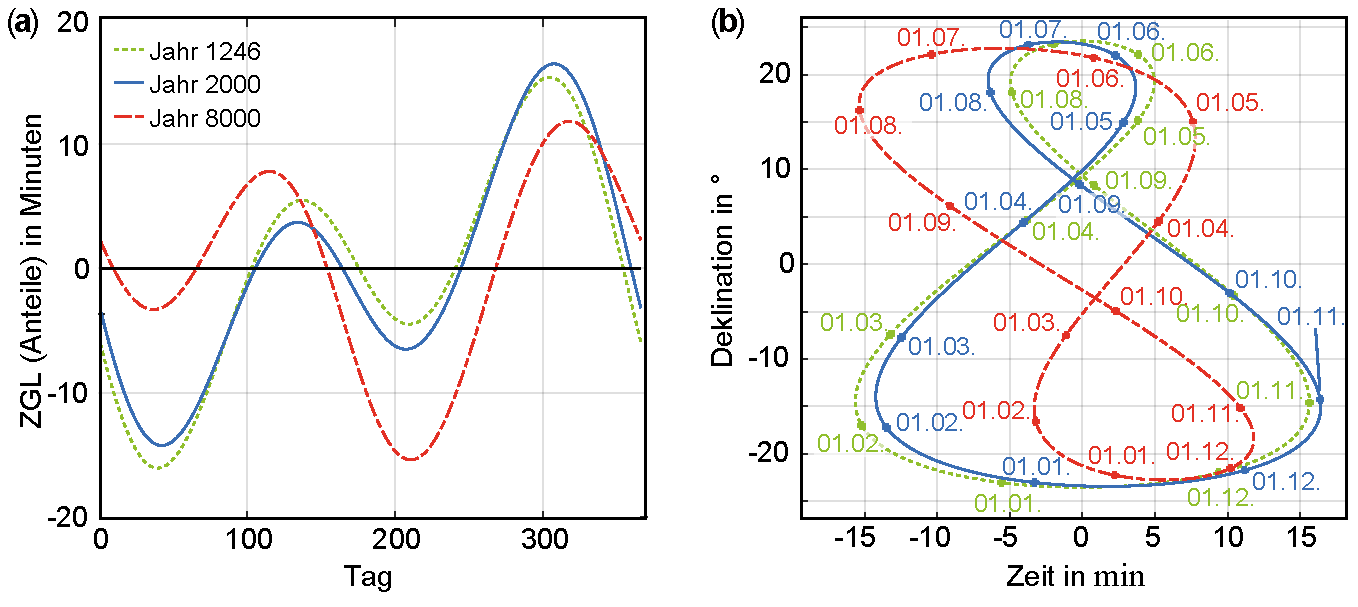
\includegraphics[width=\textwidth]{ZGL_Analemma_long.pdf}%
\caption[Zeitgleichung und Analemma f�r verschiedene Zeiten.]{\fa Zeitgleichung und \fb Analemma f�r die Jahre 1246, 2000 und 8000 u.Z.}%
\label{abb:hm_ZGL_Analemma_long}%ZGLAnnalong
\end{figure}


\subsection{Zeitr�ume von Millionen von Jahren -- Klimaeffekte}\label{kap:hm_ganz_langezeiten}

Wir wollen jetzt unser Modell noch etwas \anf{strapazieren} und auf noch l�ngere Zeiten ausdehnen.
Wir machen dabei starke Vereinfachungen hinsichtlich der Annahmen f�r die zeitlichen Entwicklung der Bahnparameter, f�r die wir einfache Periodizit�ten annehmen.
F�r die Exzentrizit�t haben wir im Mittel $e_m\!=\!0.028$ angenommen.
Dabei gibt es eine Periode von 405\,000 Jahren (Variation der Exzentrizit�t um $\pm 0.012$) und einen Zyklus von 100\,000 Jahren (Variation zwischen $-0.03$ und $+0.02$).
Ebenso nehmen wir f�r die Ekliptikschiefe eine Periodizit�t von 41\,000 Jahren um den Mittelwert $22.8\degree$ an und f�r die Perihelverschiebung einen gleichf�rmigen Zuwachs von $1.7192 \degree$ pro Jahrhundert.
\begin{figure}%
	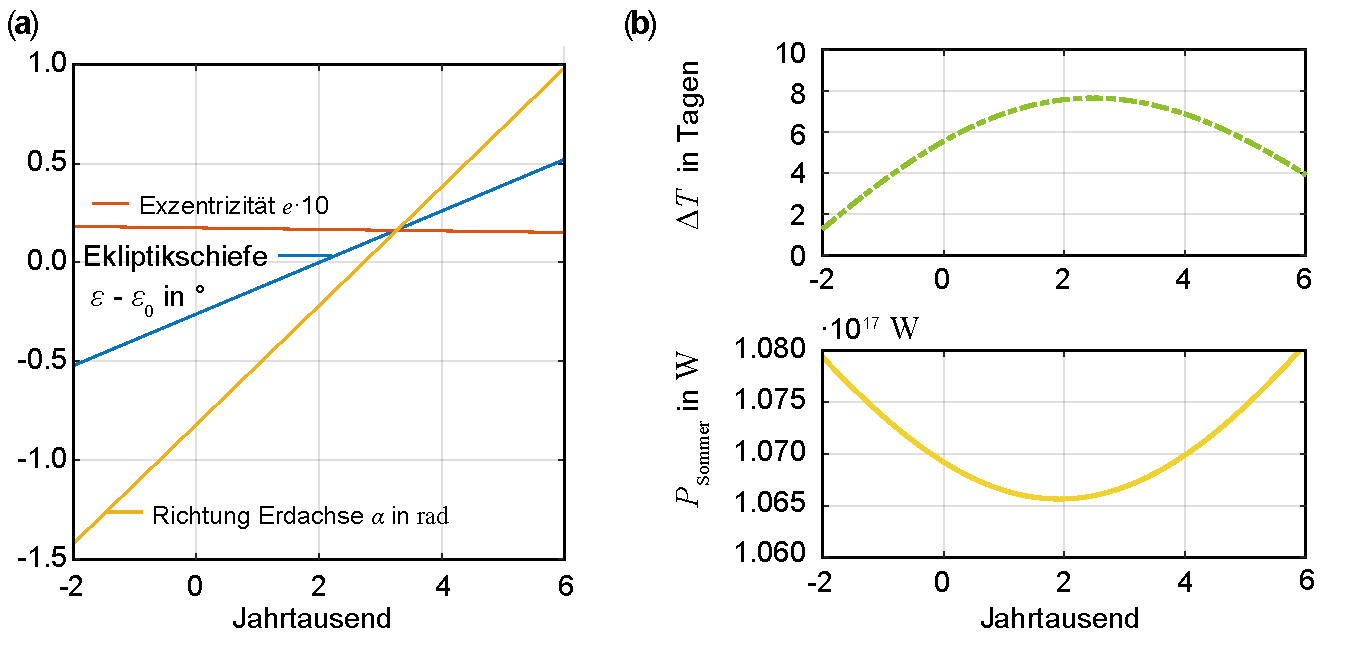
\includegraphics[width=\textwidth]{Erdbahn_im_Jahr_lsg_low.pdf}%
	\caption[Ver�nderung der Bahnparameter der Erde.]{\fa Ver�nderung der Bahnparameter der Erde �ber einen Zeitraum von 8000 Jahren und \fb Variation der Differenz UT-ET sowie der mittleren eingestrahlte Sonnenleistung auf die Nordhalbkugel in demselben Zeitraum.}
	\label{abb:hm_Nordsommer_long}%NordSommer
	\end{figure}

Wir geben hier nur unser Ergebnis der Rechnungen in \figref{hm_Nordsommer_long} an, zum Vergleich siehe auch die Ref. \cite{Rainey2022}.
Wir erkennen deutlich Periodizit�ten beim mittleren Energieeintrag.
Will man die Frage beantworten, ob diese ohne Zweifel vorhandenen (astrosolaren) Effekte einen signifikanten Einflussfaktor auf unser Klima\index{Klimaeffekt} darstellen oder vielleicht sogar dominant f�r die langfristige Entwicklung des Erdklimas mit seinem h�ufigen Wechsel von Warm- und Kaltperioden sind, dann muss man deutlich l�ngere Zeiten betrachten (\ca 1~Mio.~Jahre) und auch detailliertere Rechnungen anstellen.
Beispielsweise muss man die Verteilung von Kontinental- und Wassermassen, unterschiedliche Reflektions-, Speicher- und Abstrahlverhalten ber�cksichtigen und vor allem auch breitengradabh�ngig rechnen und nicht nur �ber die Hemisph�re integrieren.
Auf Grund von solchen (hier nur prinzipiell dargestellten) Berechnungen und deren Vergleich mit empirischen Untersuchungen des Langzeitverhaltens des Klimas ist heute im Allgemeinen anerkannt, dass die in dem \emph{Milankovic}-Zyklus\index{Milankovic-Zyklus}\footnote{Milutin Milankovic (1879--1958) war ein jugoslawischer Bauingenieur, Mathematiker und Geowissenschaftler, der als erster die Berechnung der nach ihm benannten Klima-Zyklen durchf�hrte und damit das Gebiet der der Pal�oklimatologie begr�ndete.} gezeigten periodischen Effekte mit den astronomischen Bahnparametern korrelieren (\figref{hm_Milankovic}) \cite{Milankovic1941}.
Das Bild zeigt die Variation der Erdbahnparameter, die im Vergleich zu unserem Modell deutlich pr�ziser modelliert wurden.
Gleichwohl werden die wesentlichen Effekte auch in unserem Modell sichtbar.
Vor allem periodische Ver�nderungen des solaren Energieeintrags in hohen geographischen Breiten und die Korrelation zu den beobachteten Eiszeiten kann man ableiten.
Nach der Milankovic-Theorie sind die 100\,000 Jahre-Periodizit�ten in den Eiszeiten eben durch die unterschiedliche in den h�heren Breiten im nordischen Sommer einfallende Sonnenenergie verursacht, die wiederum aus den Ver�nderungen in der Erdachsenneigung und der Perihelverschiebung\index{Perihelverschiebung} resultiert.
Allerdings hat die moderne Klimaforschung gezeigt, dass neben diesen langfristig wirkenden Klimafaktoren auch andere nat�rliche Faktoren wie Vulkanismus und die solare Aktivit�t (Sonnenflecken, Protuberanzen) wichtige Rollen spielen.
In den letzten 100--200 Jahren nimmt aber der Einfluss der anthropogenen Faktoren (Waldrodung, Kohlendioxid-Aussto� \cite{Bauer2003, Bauer2005}) signifikant zu.

	\begin{figure}%
	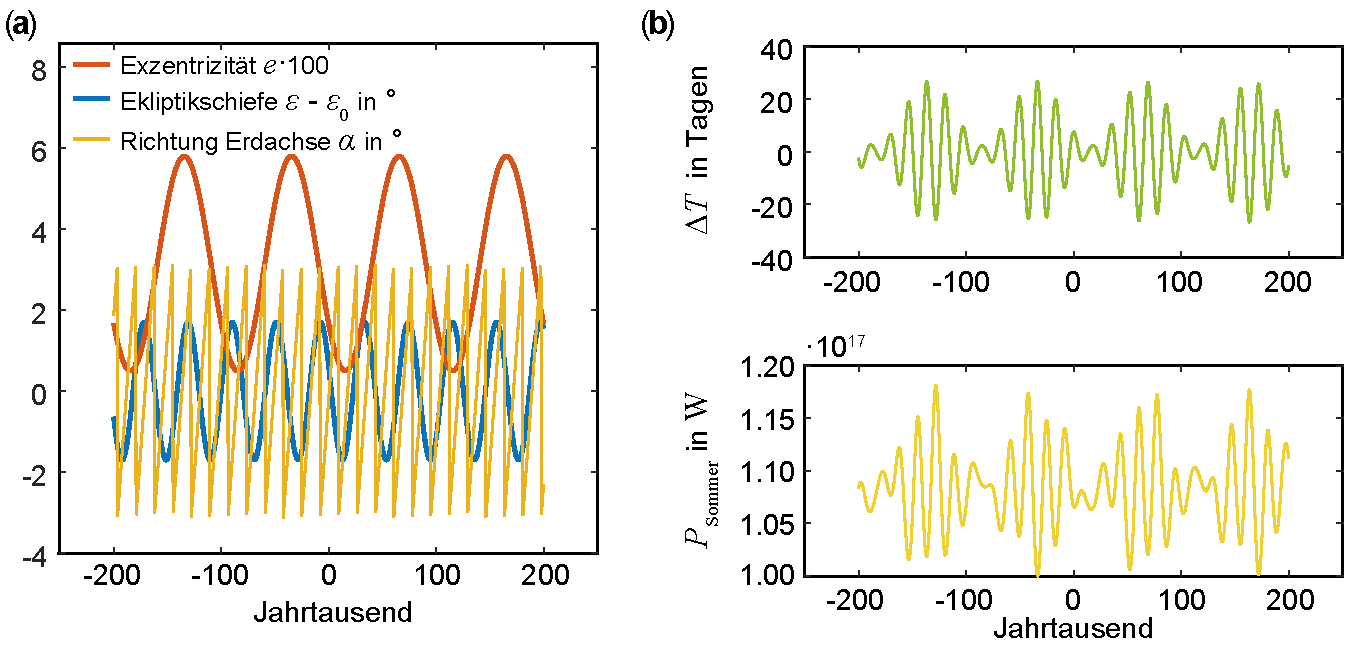
\includegraphics[width=\textwidth]{Nordsommer_long.pdf}%
	\caption[Mittlere eingestrahlte Sonnenleistung auf die Nordhalbkugel f�r sehr lange Zeiten.]{\fa Ver�nderung der Bahnparameter der Erde und \fb Variation der Differenz UT-ET sowie der mittleren eingestrahlten Sonnenleistung auf die Nordhalbkugel w�hrend des Nordsommers f�r sehr lange Zeiten.}%
	\label{abb:hm_Nordsommer_long_long}%NordSommer
	\end{figure}

	\begin{figure}%
	\centering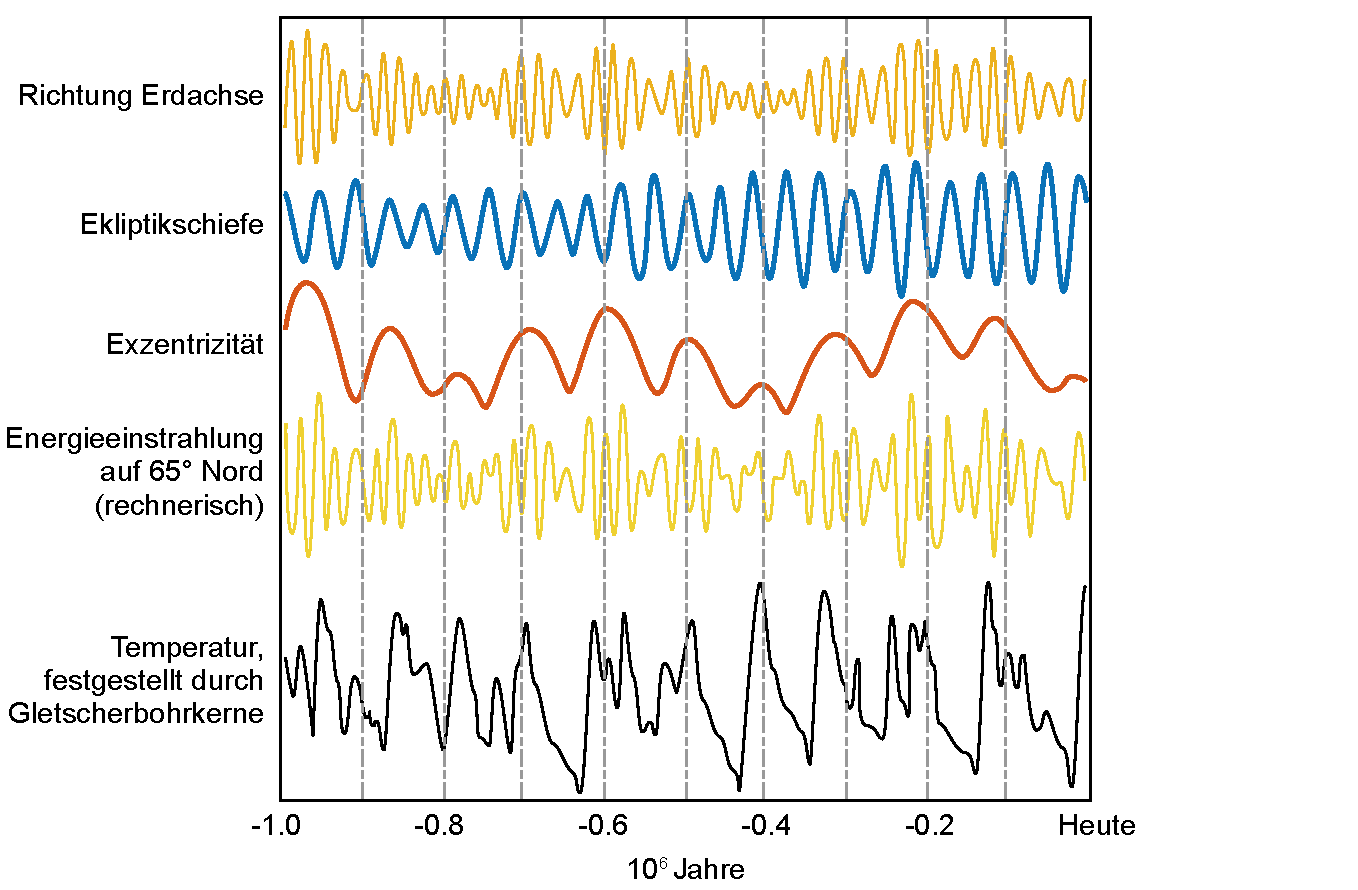
\includegraphics[width=\textwidth]{Milankovic.pdf}%
	\caption[Milankovic-Zyklen f�r einen Zeitraum von 1 Million Jahren.]{Milankovic-Zyklen f�r einen Zeitraum von 1~Mio.~Jahren \cite{Rohde2006}.
        Das Bild ist gestaltet nach einem f�r das Global Warming Art Project frei zug�nglichem Bild von Robert A. Rhode. }
	\label{abb:hm_Milankovic}%Milankovic
	\end{figure}




\clearpage
\section{Tabellen}\label{kap:hm_tabellen}

Zu weiteren in Text und �bungen verwendeten Daten siehe Tab.
\ref{tab:hm_Umrechung_KOS}, \ref{tab:hm_notation_hm},
\ref{tab:hm_bahnparameter}, \ref{tab:hm_zeitl_aenderung_bahnparameter_lin},
\ref{tab:hm_parameter_kometen}, \ref{tab:hm_parameter_halley_alt-neu},
\ref{tab:hm_parameter_shoemaker} und \ref{tab:hm_parameter_asteroide}.

\begin{sidewaystable}
\vspace{16cm}
\caption{Transformation astronomischer Koordinatensysteme.}
\smallskip
\begin{adjustbox}{width=\textwidth,totalheight=0.75\textheight,keepaspectratio}
\begin{tabular}{L{1.5cm}L{2.0cm}L{2.cm}L{6.5cm}L{6.5cm}}
\hline\noalign{\smallskip}
Umrechnung	& KOS 1 & KOS 2 & Transformation KOS 1 $\rightarrow$ KOS 2 & Transformation KOS 2 $\rightarrow$ KOS 1 \\
\noalign{\smallskip}\svhline\noalign{\smallskip}
BA $\rightarrow$ HE & Bahn & Heliozentrisch-ekliptikal & Parameter:\linebreak Bahnneigung $i$,\linebreak L�nge des aufsteigenden Knotens $\Omega$,\linebreak Argument des Perihels $\omega$ \\\\ 
 &$r$, $\upsilon$ & $l$, $b$, $r$ & $u=\upsilon+\omega$ & \\
 & & & $\cos b\cos(l-\Omega) = \cos u$ & \\
 & & & $\cos b\sin(l-\Omega) = \sin u\cos i$ & \\
 & & & $\sin b = \sin u\sin i$ & \\
\hline\noalign{\smallskip}
HE $\leftrightarrow$ GE & Heliozentrisch-ekliptikal & Geozentrisch-ekliptikal & Parameter:\linebreak heliozentrische Erdkoordinaten $R$, $L$, $B$  & Parameter:\linebreak heliozentrische Erdkoordinaten $R$, $L$, $B$ \\\\
& $l$, $b$, $r$ & $\lambda$, $\beta$, $\Delta$ & $r\cos b\cos l = R\cos B\cos L+\Delta\cos\beta\cos\lambda$ & \\
 & & & $r\cos b\sin l = R\cos B\sin L+\Delta\cos\beta\sin\lambda$ & \\
 & & & $r\sin b = R\sin B+\Delta\sin\beta$ & \\
\hline\noalign{\smallskip}
GE $\leftrightarrow$ GA & Geozentrisch-ekliptikal & Geozentrisch-�quatorial \linebreak (space-fixed) & Parameter:\linebreak  Ekliptikschiefe $\epsilon$ \vspace{\baselineskip}& Parameter:\linebreak  Ekliptikschiefe $\epsilon$ \\ \\
 & $\lambda$, $\beta$ & $\alpha$, $\delta$ & $\cos\delta\cos\alpha = \cos\beta\cos\lambda$ & $\cos\beta\cos\lambda =\cos\delta\cos\alpha$\\
 & & & $\cos\delta\sin\alpha = \cos\beta\sin\lambda\cos\epsilon-\sin\beta\sin\epsilon$ & $\cos\beta\sin\lambda =\cos\delta\sin\alpha\cos\epsilon+\sin\delta\sin\epsilon$ \\
 & & & $\sin\delta = \cos\beta\sin\lambda\sin\epsilon+\sin\beta\cos\epsilon$ & $\sin\beta = -\cos\delta\sin\alpha\sin\epsilon+\sin\delta\cos\epsilon$ \\
\hline\noalign{\smallskip}
GA $\leftrightarrow$ TA & Geozentrisch-�quatorial \linebreak (space-fixed) & Topozentrisch-�quatorial & Parameter: \linebreak Erdradius $R_\text{\earth}$, \linebreak Sternzeit $\theta$, \linebreak Geographische Breite $\varphi$, \linebreak Geozentrische Breite  $\phi =\varphi -0.1924\degree \sin(2\varphi)$, \linebreak $\rho_\text{\earth} = R_\text{\earth}-21.38 \sin^2\varphi$ \vspace{\baselineskip} & Parameter: \linebreak Erdradius $R_\text{\earth}$, \linebreak Sternzeit $\theta$, \linebreak Geographische Breite $\varphi$,\linebreak Geozentrische Breite  $\phi =\varphi -0.1924\degree \sin(2\varphi)$, \linebreak $\rho_\text{\earth} = R_\text{\earth}-21.38 \sin^2\varphi$ \vspace{\baselineskip}\\
& $\alpha$, $\delta$, $\Delta$ & $\alpha'$, $\delta'$, $\Delta'$ & $\Delta'\cos\delta'\cos\alpha' = \Delta\cos\delta\cos\alpha - \rho_\text{\earth}\cos\phi\cos\theta$ & $\Delta\cos\delta\cos\alpha = \Delta'\cos\delta'\cos\alpha' + \rho_\text{\earth}\cos\phi\cos\theta$ \\
 & & & $\Delta'\cos\delta'\sin\alpha' = \Delta\cos\delta\sin\alpha - \rho_\text{\earth}\cos\phi\cos\theta$ & $\Delta\cos\delta\sin\alpha = \Delta'\cos\delta'\sin\alpha' + \rho_\text{\earth}\cos\phi\cos\theta$ \\
 & & & $\Delta'\sin\delta' = \Delta\sin\delta - \rho_\text{\earth}\sin\theta$ \vspace{\baselineskip}& $\Delta\sin\delta = \Delta'\sin\delta' + \rho_\text{\earth}\sin\theta$ \\
 & & & N�herungen f�r $\rho_\text{\earth} \ll \Delta$: & \\
 & & & $\alpha-\alpha' = \frac{8.79''}{\Delta\lek\text{AE}\rek}\frac{\cos\phi}{\cos\delta}\sin(\theta-\alpha)\cos\delta$ & \\
 & & & $\delta-\delta' = \frac{8.79''}{\Delta\lek\text{AE}\rek}\lek\cos\delta\sin\phi -\sin\delta\cos\phi\cos(\theta-\alpha)\rek$ & \\
\hline\noalign{\smallskip}
GA $\leftrightarrow$ TH & Geozentrisch-�quatorial \linebreak (earth-fixed) & Topozentrisch-horizontal & Parameter: \linebreak Geographische Breite $\varphi$, \linebreak Stundenwinkel $\tau$ \vspace{\baselineskip}& Parameter: \linebreak Geographische Breite $\varphi$, \linebreak Stundenwinkel $\tau$ \\ \\
& $\tau$, $\delta$ & $\mathcal{A}$, $h$& $\sin h = \cos\delta\cos\tau\cos\varphi+\sin\delta\sin\varphi$ & $\sin\delta = \sin h\sin\varphi - \cos h\cos\mathcal{A}\cos\varphi$ \\
 & & & $\cos h\sin\mathcal{A} = \cos\delta\sin\tau$ & $\cos\delta\sin\tau = \cos h\sin\mathcal{A}$\\
 & & & $\cos h\cos\mathcal{A} = \cos\delta\cos\tau\sin\varphi - \sin\delta\cos\varphi$ & $\cos\delta\cos\tau = \sin h\cos\varphi + \cos h\cos\mathcal{A}\sin\varphi$\\
\noalign{\smallskip}\hline\noalign{\smallskip}
\end{tabular}
\end{adjustbox}
\label{tab:hm_Umrechung_KOS}
\end{sidewaystable}
\clearpage

\begin{table}%tab
\caption{Vergleich der in Physik und Himmels\-me\-cha\-nik/As\-tro\-no\-mie �blichen Notationen f�r das Zweik�rperproblem.}
\smallskip
\begin{tabular}{L{3.6cm}L{4.3cm}L{4.1cm}}
Physikalisch-  \linebreak Mathematische Gr��e	&	 Physikalische Notation\linebreak Band I	& Astronomische Notation \linebreak \autoref{chap:hm} \linebreak Spezifische Gr��en, \dh auf die Masse $m$ bezogen.\\ \\
\noalign{\smallskip}\hline\noalign{\smallskip}
\smallskip
& & \\
Effektive Masse	&$m_\text{eff} = \dfrac{m_1m_2}{m_1+m_2}$	&$m_\text{eff} = 1$	\\	\\
Gravitationspotential	&$U(r) = -\dfrac{\kappa}{r} = -\dfrac{G m_1 m_2}{r}$	&$U(r) = -\dfrac{\mu_\text{G}}{r} = -\dfrac{G (m_1 + m_2)}{r}$\\	\\
Energie	&$E = \dfrac{1}{2}  m_\text{eff}\: \dot{r}^2 \!+\! \dfrac{L}{2  m_\text{eff}\: r^2} \!+\! U(r)$ & $H = \dfrac{1}{2} \dot{r}^2 + \dfrac{L}{2\, r^2} + U(r)$	\\	\\
Drehimpuls	&$L = m_\text{eff}\: r^2 \dot{\varphi}$&$L = r^2 \dot{\upsilon}$	\\	\\
Numerische Exzentrizit�t &$\epsilon = \sqrt{\dfrac{2 E L^2} {m_\text{eff}\: \kappa^2}}$&$e = \sqrt{\dfrac{2 H L^2}{\mu_\text{G}^2} + 1} $ \\ \\
Bahnparameter  &$p = \dfrac{ L^2}{ m_\text{eff}\: \kappa}$&$p = \dfrac{ L^2}{ \mu_\text{G}} $\\ \\
Gro�e Halbachse  &$a = \dfrac{p}{1-\epsilon^2}$ & $a = \dfrac{p}{1-e^2} $ \\ \\
Wahre Anomalie  &$\varphi$ &$\upsilon$ \\ \\
Exzentrische Anomalie & - &$E$ \\ \\
\noalign{\smallskip}\hline\noalign{\smallskip} \\
\end{tabular}\\ 
\label{tab:hm_notation_hm}
\end{table}

\begin{table}%tab6
\caption{Mittlere Bahnparameter der Planeten unseres Sonnensystems.}
\smallskip
\begin{adjustbox}{width=\textwidth,totalheight=\textheight,keepaspectratio}
\begin{tabular}{L{1.3cm}R{1.3cm}R{1.3cm}R{1.2cm}R{1.5cm}R{1.5cm}R{1.6cm}R{1.4cm}R{1.5cm}}
\multicolumn{8}{l}{\textbf{Bezug: �quinoktium und Ekliptik des Datums}\cite{Meeus1998}.} \\
\hline\noalign{\smallskip}
Element					& $a$ \;\   & $e$ \;\ & $i$ \;\            & $\Omega$ \;\       & $\varpi$ \;\       & $M_0$ \;\          & $L_0$ \;\          & $n_\text{anom}$ \;\ \\
Einheit					& in AE \;\ &         & in \textdegree \;\ & in \textdegree \;\ & in \textdegree \;\ & in \textdegree \;\ & in \textdegree \;\ & in \textdegree/Jh. \;\ \\
\noalign{\smallskip}\svhline\noalign{\smallskip}
Merkur \mercury & 0.387089 & 0.205631 & 7.004986& 48.330893	&  77.456119 & 174.794787	& 252.250906&149473.269\\
Venus \venus		&	0.723329 & 0.006772 & 3.394662& 76.679920	& 131.563703 &  50.416098	& 181.979801& 58518.220\\
Erde \earth 		& 1.000000 & 0.016709 & 0.000000& 0.000000	& 102.937348 & 357.529109	& 100.466457& 35999.371\\
Mars \mars			& 1.523679 & 0.093401 & 1.849726& 49.558093	& 336.060234 &  19.372766	& 355.433000& 19140.563\\
Jupiter \jupiter&	5.202603 & 0.048497 & 1.303267& 100.464407&  14.331207 &  20.020312	&  34.351519&  3033.639\\
Saturn \saturn	&	9.554909 & 0.055548 & 2.488879& 113.665503&  93.057237 & 317.020207	&  50.077444&  1218.864\\
Uranus	\uranus	&	19.218446& 0.046381 & 0.773197& 74.005957 & 173.005291 & 141.049714	& 314.055005&   427.285\\
Neptun	\neptune&	30.110387	& 0.009456 & 1.769953& 131.784057& 48.120276 & 256.228389	& 304.348665&   217.882\\
Pluto \pluto		&	39.481687 & 0.248808 & 17.14175& 110.303470&224.066760 &  14.86205	& 238.928810&   145.112\\
\noalign{\smallskip}\hline\noalign{\smallskip} \\
\end{tabular} 
\end{adjustbox}
\vspace{0.5cm}
\begin{adjustbox}{width=\textwidth,totalheight=\textheight,keepaspectratio}
\begin{tabular}{L{1.3cm}R{1.3cm}R{1.3cm}R{1.2cm}R{1.5cm}R{1.5cm}R{1.6cm}R{1.4cm}R{1.5cm}}
\multicolumn{8}{l}{\textbf{Bezug: �quinoktium und Ekliptik J2000}\cite{Montenbruck1999, Standish1992, Murray2008}.} \\
\hline\noalign{\smallskip}
Element					& $a$ \;\   & $e$ \;\ & $i$ \;\            & $\Omega$ \;\       & $\varpi$ \;\       & $M_0$ \;\          & $L_0$ \;\          & $n_\text{anom}$ \;\ \\
Einheit					& in AE \;\ &         & in \textdegree \;\ & in \textdegree \;\ & in \textdegree \;\ & in \textdegree \;\ & in \textdegree \;\ & in \textdegree/Jh. \;\ \\
\noalign{\smallskip}\svhline\noalign{\smallskip}
Merkur \mercury & 0.387098 &	0.20563069 & 7.00487	& 48.33167	&  77.45645 & 174.79439 & 252.25084	&	149473.095	\\
Venus \venus		&	0.723332 &	0.00677323  & 3.39471	& 76.67922	& 131.53298	&  50.44675 & 181.97973	&	 58517.8572	\\
Erde \earth 		& 1.000000 &	0.01671022 & 0.00005	& 174.873176	& 102.94719	& 357.51716 & 100.46435	&	 35999.3719	\\
Mars \mars			& 1.523662 &	0.09341233	 & 1.85061	& 49.57854	& 336.06020	&  19.39312 & 355.45332	&	 19140.877	\\
Jupiter \jupiter&	5.203363 &	0.04839266 & 1.30531	& 100.55615	& 14.75385	&  19.65053 &  34.40438	&	  3032.974\\		
Saturn \saturn	&	9.537070 &	0.0541506  & 2.48446	& 113.71504	& 92.43194	& 317.51238 &  49.94432	&	  1222.285\\
Uranus	\uranus	&	19.191264 &	0.0471771 & 0.76986	& 74.22988	& 170.96424	& 142.26794 & 313.23218 &	   4286.193\\
Neptun	\neptune&	30.068964	& 0.008589 & 1.76917	& 131.72169	& 44.97135	& 259.90868 & 304.88003	&	   218.332\\	
Pluto \pluto		&	39.481687 &	0.2488077 & 17.14175	& 110.30347	& 224.06676	&  14.86205 & 238.92881	&	   145.112 \\
\hline
%\noalign{\smallskip}
\end{tabular}
\end{adjustbox}
Die Parameter beziehen sich auf das �quinoktium und die Ekliptik des Datums bzw. das �quinoktium und die Ekliptik der Standardepoche J2000 \cite{Standish1992, Murray2008, Meeus1998}.
Im letzteren Fall gelten die f�r die Erde gelisteten Werte f�r den Erde-Mond-Schwerpunkt.\\
F�r die Epoche J2000 gilt $\epsilon\!=\!23.4392911\degree$.
Die gro�e Halbachse $a$ ist in Astronomischen Einheiten ($1\:\text{AE}= 149597870700\:\text{m}$) angegeben, alle Winkel in $\degree$.
Das Perihelargument $\omega$ wird in der Bahnebene vom aufsteigenden Knoten bis zum Perihel gemessen.
Die L�nge des Perihels $\varpi$ wird in der Ekliptik vom Fr�hlingspunkt bis zum aufsteigenden Knoten und dann in der Bahnebene des Himmelsk�rpers vom aufsteigenden Knoten bis zum Perihel gemessen ($\varpi\!=\!\Omega+\omega$).
Die mittlere t�gliche Bewegung $n$ (mittlere Umlaufgeschwindigkeit) wird in Grad pro Jahrhundert angegeben.
Die mittlere L�nge $L_0$  wird in der Ekliptik vom Fr�hlingspunkt bis zur mittleren Position des Planeten gemessen.
Statt der mittleren L�nge wird oft die mittlere Anomalie $M_0$ angegeben (Vergleiche auch dazu \figref{hm_planetenbahnen_rel_ekliptik}). 
Wir haben in der Tabelle f�r die inneren Planeten die mittleren Bahnelemente angegeben, d.\,h. die Elemente f�r ein reines ZKP.
Bei den �u�eren Planeten (ab Jupiter) sind die Einfl�sse der anderen Planeten so gro�, dass man deshalb f�r diese Planeten j�hrliche, aktuelle Bahnelemente angibt, die mit Methoden der St�rungsrechnung berechnet werden.
F�r unsere Zwecke k�nnen wir aber mit \anf{mittleren} Bahnelementen rechnen.
Obwohl seit dem 24.08.2006 die \href{https://de.wikipedia.org/wiki/Internationale_Astronomische_Union}{Internationale Astronomische Union (IAU)} durch eine pr�zisere Begriffsdefinition f�r Planeten den Pluto nur noch in der Kategorie Zwergplanet f�hrt, haben wir aus Nostalgiegr�nden (Merksatz in der Schule: \anf{\emph{M}it \emph{V}iel \emph{E}lan \emph{M}urmelt \emph{J}eder \emph{S}ch�ler \emph{U}nsere \emph{N}eun \emph{P}laneten}) in der Tabelle den Pluto mit als Planet aufgef�hrt.\\ \\
Die Daten der Tabelle \ref{tab:hm_bahnparameter} sind in den Dateien \mlhmdref{Bahnparameter.csv} bzw. \mlhmdref{BahnparameterJ2000.csv} gespeichert.
Die Daten f�r den Mars sind aus \cite{Allison2000} entnommen.
\label{tab:hm_bahnparameter}
\end{table}

\begin{table}%tab7
\caption{Linearer Term der zeitlichen Ver�nderung der Bahnparameter.} 
\smallskip
\begin{tabular}{L{1.3cm}R{1.5cm}R{1.5cm}R{1.2cm}R{1.2cm}R{1.2cm}R{1.7cm}R{1.7cm}}
\multicolumn{8}{l}{\textbf{Bezug: �quinoktium und Ekliptik des Datums }\cite{Meeus1998}.} \\
\hline\noalign{\smallskip}
Element	\linebreak Einheit	& $\dot{a}$ \linebreak $\times 10^{-8}\linebreak \text{AE}/\text{Jh.}$	& $\dot{e}$	\linebreak $\times 10^{-8} \linebreak \text{AE}/\text{Jh.}$& $\d i/\d t$	& $\dot{\varpi}$	& $\dot{\Omega}$	& $\dot{L}_0$ \linebreak $= n_\text{trop}$& $\dot{M}_0$ \linebreak $= n_\text{anom}$\\
\noalign{\smallskip}\svhline\noalign{\smallskip}
Merkur \mercury		& 66 			& 2527 		& 0.0018  	& 1.5555  & 1.1862  & 149474.0710 	& 149472.5150 \\
Venus \venus 			& 92 			& -4938 	& 0.0010  	& 1.4080  & 0.9011  & 58319.2119 		& 58517.8039 \\
Erde \earth 			& -5 			& -3804 	& 0.0000  	& 1.7195  & 0.0000  & 36000.7690  	& 35999.0498 \\
Mars \mars				& -7221 	& 11902 	& -0.0006  	& 1.8408  & 0.7721  & 19140.5028  	& 19139.8585 \\
Jupiter \jupiter	& 60737 	& -12880 	& -0.0055  	& 1.6126  & 1.0210  & 3034.9057  		& 3033.6272 \\
Saturn \saturn 		& -301530 & -36762 	& -0.0037  	& 1.9638  & 0.8771  & 1222.1138  		& 1213.8664 \\
Uranus \uranus    & 152025 	& -19150 	& 0.0008  	& 1.4864  & 0.5211  & 428.467  		& 426.9282 \\
Neptun \neptune 	& -125196 & 2514 		& -0.0093 	& 1.4263  & 1.1022  & 218.4862 		& 217.9599 \\
Pluto \pluto    	& -125196 & 2514 		&  	&   & 0 & 145.2078  		& 143.7818 \\
\noalign{\smallskip}\hline\noalign{\smallskip} \\
\end{tabular} 
\vspace{0.5cm}
\begin{tabular}{L{1.3cm}R{1.5cm}R{1.5cm}R{1.2cm}R{1.2cm}R{1.2cm}R{1.7cm}R{1.7cm}}
\multicolumn{8}{l}{\textbf{Bezug: �quinoktium und Ekliptik J2000}\cite{Standish1992, Murray2008}.} \\
\hline\noalign{\smallskip}
Element	\linebreak Einheit	& $\dot{a}$ \linebreak $\times 10^{-8}\linebreak \text{AE}/\text{Jh.}$	& $\dot{e}$	\linebreak $\times 10^{-8}\linebreak \text{AE}/\text{Jh.}$& $\d i/\d t$	& $\dot{\varpi}$	& $\dot{\Omega}$	& $\dot{L}_0$ \linebreak $= n_\text{trop}$& $\dot{M}_0$ \linebreak $= n_\text{anom}$\\
\noalign{\smallskip}\svhline\noalign{\smallskip}
Merkur \mercury		& 66 			& 2527 		& -0.0065  & 0.1593  & -0.1254  & 149472.6738  & 149472.5153 \\
Venus \venus			& 92 			& -4938 	& -0.0008  & 0.0049  & -0.2780  & 58317.8149   & 58517.8039 \\
Erde \earth				& -5 			& -3804 	& -0.0130  & 0.3226  & -0.2411  & 35999.3720   & 35999.0498 \\
Mars \mars				& -7221 	& 11902 	& -0.0071  & 0.4439  & -0.2950  & 19140.5061   & 19139.8572 \\
Jupiter \jupiter 	& 60737 	& -12880	& -0.0012  & 0.2156  & 0.1767   & 3034.9057    & 3033.6272 \\
Saturn \saturn		& -301530 & -36762 	&  0.0017  & 0.5665  & -0.2567  & 1222.1138    & 1213.8664 \\
Uranus \uranus 		& 152025 	& -19150 	& -0.0006  & 0.0893  & 0.0741   & 428.4670     & 426.9282 \\
Neptun \neptune 	& -125196 & 2514 		& -0.0009  & 0.0292  & -0.0062  & 219.8833  		& 217.9599 \\
Pluto \pluto 			& -76912  & 6465 		&  0.3075  & 1.4263  & -0.0104  & 145.2078	 	& 143.7818 \\
\noalign{\smallskip}\hline\noalign{\smallskip} \\
\end{tabular}
Die Parameter beziehen sich auf das �quinoktium des Datums bzw. das �quinoktium und die Ekliptik der Standardepoche J2000.
Im letzteren Fall gelten die f�r die Erde gelisteten Werte f�r den Erde-Mond-Schwerpunkt. Alle Einheiten au�er f�r $\dot{a}$ und $\dot{e}$ sind in $\degree/\text{Jh.}$ angegeben.\\ \\
Die Bahnparameter als Funktion der Zeit $t$  (in Julianischen Jahrhunderten) berechnen sich zu: $x(t)\!=\!x+\dot{x}\,t$.\\ \\
Es sei darauf hingewiesen, dass die ersten f�nf Spalten der Tabelle tats�chlich zeitliche Ver�nderungen der Bahnparameter darstellen, w�hren die beiden letzten Spalten f�r $\dot{L}_0$ und $\dot{M}_0$ die L�nge bzw. Mittlere Anomalie des Perihels beschreiben und daher eigentlich Umlaufgeschwindigkeiten f�r die mittlere Bewegung $n$\index{Bewegung!mittlere|textbf} darstellen. \\
Die zeitliche Ver�nderung der Ekliptikschiefe $\epsilon$ kann wie folgt beschrieben werden:\\ 
$\epsilon\!=\!23.4392911\degree-46.8150''\,t-0.00059''\,t^2 + 0.001813''\,t^3$. \\ \\
Die Daten f�r den Mars sind aus \cite{Allison2000} entnommen.
Die Daten der Tabelle \ref{tab:hm_zeitl_aenderung_bahnparameter_lin} sind in den Dateien \mlhmdref{BahnparameterAbleitung.csv} bzw. \mlhmdref{BahnparameterJ2000Ableitung.csv} gespeichert.
\label{tab:hm_zeitl_aenderung_bahnparameter_lin}
\end{table}

\begin{table}%tab8
\caption{Parameter ber�hmter Kometen \cite{JPL2020}.}
\smallskip
\begin{tabular}{L{1.2cm}C{1.8cm}C{2.7cm}C{2cm}C{2cm}L{1.3cm}}
\hline\noalign{\smallskip}
Element				& Gro�er Komet \linebreak (1680) & Komet Halley \linebreak (1986)	& Komet Neowise \linebreak (2020) & Komet Donati \linebreak (1858) &	Einheit \\
\noalign{\smallskip}\svhline\noalign{\smallskip}
$e$						&	0.999986			&	0.967142908462304 & 0.999188062	& 0.996295 &	\\		
$a$						&	444.4285714		&	17.8341442925537	& 362.8965186	& 156.1319838 &	AE \\	
$q$						&	0.006222			&	0.585978111516909	& 0.294649337 & 0.578469 & AE	\\	
$i$						&	60.6784				&	162.262690579161	& 128.9372925	& 116.9512 & Grad (\textdegree)	\\	
$\Omega$			&	276.6339			&	58.42008097656843 & 61.01054495	& 167.3044	&	Grad (\textdegree)	\\	
$\omega$			&	350.6128			&	111.3324851045177	& 37.27889887	& 129.1144	&	Grad (\textdegree)			\\	
$M$						&	-0.0020500		&	38.3842644764388	& 0.001328884	& 0.003807	&	Grad (\textdegree)			\\	
$t_0$					&	2335019.9876	&	2446467.3953170509 & 2459034.179 & 2399952.965 & TT	\\	
							&1680-Dec-18.4876 & 1986-Feb-\linebreak 05.89539 & 2020-Jul-03.67911 & 1858-Sep-30.4645 & \\
$T_\text{P}$	&	---					&	75.31589278				& 6913.25			& --- 	&	Jahre			\\	
$n$						&	0.0001052			&	0.0130865647924		& 0.000142571		& 0.0005052	&	Grad/Tag $\lk \degree/\text{d} \rk$	\\	
$Q$						&	888.850				&	35.0823						& 725.499			& 311.685 & AE\\
\noalign{\smallskip}\hline\noalign{\smallskip}
\end{tabular} \\
\label{tab:hm_parameter_kometen}
\\
Die Bahnelemente beziehen sich auf die Epoche des Periheldurchgangsdatums im Koordinatensystem von �quinoktium und Ekliptik von J2000. Die mittlere Bewegung $n$ \index{Bewegung!mittlere} ist in Grad pro Tag angegeben \cite{JPL2020}.
\end{table}

\begin{table}%tab9
\caption{Vergleich Parameter des Kometen Halley f�r verschiedene Epochen (1758 und 1986) \cite{JPL2020}.}
\smallskip
\begin{tabular}{L{1.2cm}C{3cm}C{3cm}L{2cm}}
\hline\noalign{\smallskip}
Element			&	Komet Halley \linebreak (1986)  	& Komet Halley \linebreak (1758)	&	Einheit \\
\noalign{\smallskip}\svhline\noalign{\smallskip}
$e$						&	0.967142908462304	&	0.967686 &		---				\\	
$a$						&	17.8341442925537	&	--- &	AE			\\	
$q$						& 0.585978111516909		&	0.584466 &	AE				\\	
$i$						&	162.262690579161		&	162.372 & Grad (\textdegree)	\\	
$\Omega$			&	58.42008097656843		&	57.2458 &	Grad (\textdegree)	\\	
$\omega$			&	111.3324851045177		&	110.7093	& Grad (\textdegree)			\\	
$M$						&	38.3842644764388		&	--- &	Grad (\textdegree)			\\	
$t_0$					&	2446467.39531705092		&	2363592.5623 & TT				\\	
							& 1986-Feb-05.89539 & 1759-Mar-13.06230 & \\
$T_\text{P}$	&	75.31589278					& ---	& Jahre				\\	
$n$						&	0.0130865647924		& ---  &	Grad/Tag $\lk \degree/\text{d} \rk$				\\	
$Q$						&	35.0823 	& ---	&	AE		\\
\noalign{\smallskip}\hline\noalign{\smallskip}	
\end{tabular}\\
\label{tab:hm_parameter_halley_alt-neu}
Die Bahnelemente beziehen sich auf die Epoche des Periheldurchgangsdatums im Koordinatensystem von �quinoktium und Ekliptik von J2000.
\end{table}


\begin{table}%tab10
\caption{Wesentliche Parameter des Kometen Shoemaker-Levy 9\index{Komet!Shoemaker-Levy} (2 Bruchst�cke) \cite{JPL2020}.}
\smallskip
\begin{tabular}{L{1.2cm}C{3cm}C{3cm}L{2cm}}
\hline\noalign{\smallskip}
Element			&	D/1993 F2-D \linebreak Shoemaker-Levy 9		& D/1993 F2-A \linebreak Shoemaker-Levy 9	&	Einheit \\
\noalign{\smallskip}\svhline\noalign{\smallskip}
$e$						&	0.214725345	&	0.216209167 &		---				\\	
$a$						&	6.851576928		&	6.864794628 &	AE			\\	
$q$						& 5.38036971		&	5.3805631 &	AE				\\	
$i$						&	5.972967603		&	6.003293874& Grad (\textdegree)	\\	
$\Omega$			&	220.6003061		&	220.537655 &	Grad (\textdegree)	\\	
$\omega$			&	354.9131083		&	354.8935192	& Grad (\textdegree)			\\	
$M$						&	2.412564931		&	2.460243948 &	Grad (\textdegree)			\\	
$t_0$					&	2449436.6 		&	2449435.603 & TT				\\	
							& 1994-Mar-25.1003817 & 1994-Mar-24.1031964 & \\
$T_\text{P}$	&	17.93 					& 17.99				& Jahre				\\	
$n$						&	0.054956399		&	0.054797753 &	Grad/Tag $\lk \degree/\text{d} \rk$				\\	
$Q$						&	8.322784146 	&	8.349026155	&	AE		\\
\noalign{\smallskip}\hline\noalign{\smallskip}	
\end{tabular}\\
Die Bahnelemente beziehen sich auf die Epoche des Periheldurchgangsdatums im Koordinatensystem von �quinoktium und Ekliptik von J2000.
\label{tab:hm_parameter_shoemaker}
\end{table}

\begin{table}%tab11
\caption{Wesentliche Parameter der Asteroiden 268057 und 103770 \cite{JPL2020}.}
\smallskip
\begin{tabular}{L{1.2cm}C{3cm}C{3cm}C{3cm}L{2cm}}
\hline\noalign{\smallskip}
Element	&	Asteroid 231937 \linebreak (2001 FO32)	&	Asteroid 268057 \linebreak Michaelkaschke \linebreak (2004 RQ24)	& Asteroid 103770 \linebreak Wilfriedlang \linebreak (2000 DP1)	&	Einheit \\
\noalign{\smallskip}\svhline\noalign{\smallskip}
$e$					&	0.8261262239	&	0.082402561	&	0.126261549 &		---				\\	
$a$					&	1.7011287637	&	2.807169394		&	3.139173278 &	AE				\\	
$q$					&	0.2957816817	&	2.575851446		&	2.742816397 &	AE				\\	
$i$					&	38.981921719	&	3.265048167		&	16.5770908 & Grad (\textdegree)	\\	
$\Omega$		&	181.73154319	&	270.5748039		&	358.5446343 &	Grad (\textdegree)	\\	
$\omega$		&	123.31366145	&	113.4224849		&	218.2774378	& Grad (\textdegree)			\\	
$M$					&	299.160042891	&	101.9754001		&	198.1967447 &	Grad (\textdegree)			\\	
$t_0$				&	2459337.45901	&	2458513.875 	&	2459913.574 & TT				\\	
						&	2021-May-02.95900974 & 2019-Jan-30.37515943 & 2022-Nov-30.07429017 & \\
$T_\text{P}$	&	2.22	&	4.7 					& 5.56				& Jahre				\\	
$n$					&	0.4422018838	&	0.209556504		&	0.177207109 &	Grad/Tag $\lk \degree/\text{d} \rk$				\\	
$Q$					& 3.10647584585	&	3.038487342 &	3.53553015	&	AE		\\
\noalign{\smallskip}\hline\noalign{\smallskip}	
\end{tabular}\\ 
Die Bahnelemente beziehen sich auf die Epoche des Periheldurchgangsdatums im Koordinatensystem von �quinoktium und die Ekliptik von J2000.\\ \\
Der Asteroid 231937 (2001 FO32) kam im Jahre 2021 der Erde relativ nahe (siehe \mlhmref{AsteroidenZeit.m}). 
\label{tab:hm_parameter_asteroide}
\end{table}



\clearpage
\renewcommand\glslongextraNameAlign{p{36mm}}
\renewcommand\glslongextraDescAlign{p{60mm}}
\clearpage
\bgroup
\small
\printunsrtglossary[type=hm]
\egroup
\clearpage
\fancyhead[RE]{\nouppercase\rightmark}
\begingroup
\let\cleardoublepage\relax
\bibliography{referenzen}
\endgroup
\fancyhead[RE]{\nouppercase\leftmark}
%%%%%%%%%%%%%%%%%%%%%%%%%%%%%%%%%%%%%%%%%%%%%%%%%%%%%%%%%%%%%%%%%%%%%%%%%%%
%\IfFileExists{footer.tex}{\input{footer.tex}}{}
